%		UEBER DIESES DESIGN
%	
%	Dieses Vorlesungsskript soll dem Layout eines Buches entsprechen und alles beinhalten, 
%	was man fuer eine Mathevorlesung brauchen koennte. Ich habe mich fuer eine KOMA Script 
%	Klasse entschieden, einfach weil sie Optioen bieten, die man bei den Standardklassen 
%	nur ueber Umwege erreichen konnte. Der Code ist teilweise von mir selbst, teilweise aus 
%	allen moeglichen Quellen zusammengekratzt, ich habe mich bemueht ihn so sehr ich kann 
%	zu kommentieren.
%	Ich bin kein Experte fuer Typographie, alles wurde zwar nach meinem besten Gewissen getan, 
%	aber wenn jemand anderer Meinung ist, dann waere ich froh, wenn er meine Fehler korrigieren
%	koennte.
%
%		FEATURES DIE ICH GERNE NOCH HAETTE
%	* besseres Beweisende: das Kaestchen am Ende eines Beweises steht auf der gleichen Zeile 
%		wie die letzte Zeile. Es sollte eine Zeile tiefer 

\documentclass[a4paper, 12pt, numbers=noendperiod, chapterprefix=true]{scrbook}
% "numbers=noendperiod" macht dass beim Kapteln und aehnlichem kein Punkt am Ende steht
% normalerweise ist der Vorgang automatisiert, aber bei mir versagt es. ich mache die
% Punkte spaeter dann per hand wenn es sein muss.

% "chapterprefix=true" macht dass Kapitel, Abschnitte und aehnliches immer eine Ueber-
% schrift wie "Kapitel 1" hat. Gilt auch fuer den Anhang.

% Meta-Daten fuer Latexki
\usepackage{latexki}
\lecturer{Prof. Dr. F. Herrlich}
\semester{Wintersemester 11/12}
\scriptstate{complete}



% Nummerierung der Paragraphen anpassen (sonst kommt etwas wie "Definition 2.9.1" heraus)
\renewcommand{\thesection}{\arabic{section}}

% Deutsche Sprache
\usepackage{ngerman}

% Verschiebt \sections auf die naechste seite falls sie zu tief sind. Muss vor
% hyperref kommen.
\usepackage[nobottomtitles]{titlesec}

%Meta-Daten fuer Latexki (nur fuer das Mitschriebwiki interessant; kann ansonsten auskommentiert werden)
\usepackage{latexki}
\lecturer{Prof. Dr. F. Herrlich}
\semester{Wintersemester 2011/12}
\scriptstate{complete}


% Schicke Schrift
\usepackage[utf8]{inputenc}
\usepackage[T1]{fontenc}
\usepackage{lmodern}

% Einheitliche Schriftart (KOMA Script verwendet fuer einige Ueberschriften eine serifenlose Schrift, mischt also
% Schriftarten. Ich habe mir die Argumente dafuer durchgelsen und war nicht ueberzeugt. Wenn jemand, der mehr als
% ich von der Materie versteht, anderer Meinung ist kann er diese Zeilen hier einfach auskommentieren)
\setkomafont{chapter}{\Huge\bfseries\rmfamily}
\setkomafont{chapterentry}{\bfseries\rmfamily}
\setkomafont{disposition}{\bfseries\rmfamily}
\setkomafont{descriptionlabel}{\bfseries\rmfamily}

%Stellt das Paragraphenzeichen vor die Section-Nummer (das ist ein KOMA Script exklusiver Befehl)
% \ifstr{#1}{section} ueberprueft, ob der erste parameter (also die erste Ebene der Ueberschrift)
% section heisst, wenn ja, dann wird sie geaendert, ansonsten behalten wir den Standard
\renewcommand*{\othersectionlevelsformat}[3]{\ifstr{#1}{section}{\S\ #3\autodot}{#3\autodot}\enskip}

%Aendert die Kapitelbeschriftung in der Kopfzeile der linken Seiten
\renewcommand*{\chaptermarkformat}{\chapappifchapterprefix{\ }\thechapter\autodot:\enskip}

%Stellt ein Pragraphenzeichen vor den Abschnitt in der Kopfzeile der linken Seiten
\renewcommand*{\sectionmarkformat}{\S \thesection\autodot\enskip}

% schmaler rand
\usepackage{geometry}
\geometry{a4paper,tmargin=2cm,lmargin=2cm,rmargin=2cm}

\setlength\parskip{\smallskipamount}
\setlength\parindent{0pt}
\tolerance=900

% Index erzeugen
\usepackage{index}
\newindex{default}{idx}{ind}{Stichwortverzeichnis}

% links
\usepackage{color}
\usepackage{hyperref}

\definecolor{rltred}{rgb}{0.75,0,0}
\definecolor{rltgreen}{rgb}{0,0.5,0}
\definecolor{rltblue}{rgb}{0,0,0.75}

\hypersetup{
  pdftitle={Algebraische Geometrie Prof. Herrlich},
  pdfsubject={Algebraische Geometrie},
  pdfkeywords={Algebraische Geometrie Herrlich},
  pdfproducer={pdfLaTeX},
  pdfpagemode={UseOutlines},
  colorlinks=true,
  bookmarksopen=true,
  bookmarksnumbered=true,
  urlcolor=rltblue,
  filecolor=rltgreen,
  linkcolor=rltblue,
  backref=true,
  pagebackref=true,
  pdfpagemode=None
}

% um Code schreiben zu koennen
\usepackage{listings}

% Mathe-Pakete
\usepackage{amssymb}
\usepackage{amsmath}
\usepackage{amsfonts}
\usepackage{stmaryrd}

% F\"ur TikZ-Diagramme
\usepackage{tikz}
\usetikzlibrary{matrix,arrows,calc}
\usetikzlibrary{decorations.text}

% Verschiedene items in enumerate Umgebungen (Das enumitem Paket bietet mehr Optionen)
\usepackage{enumerate}

% Erweiterte description umgebung
\usepackage{expdlist}

%fuer schoene Brueche
\usepackage{nicefrac}

% fuers Durchstreichen
\usepackage[normalem]{ulem}

% Fuer Diagramme
\usepackage[arrow,matrix,curve]{xy}

\usepackage{etex}
\usepackage{pictex}
\usepackage{graphicx}

% Theorem-Umgebung
\usepackage[hyperref,amsmath,thmmarks,thref]{ntheorem}

% Fuer verlaengerte Pfeile
\usepackage{extarrows}

% keine kursiv schrift in theorems
\theorembodyfont{}

% Theoreme definieren
\theoremstyle{break}
	\newtheorem{Satz}{Satz}
	\newtheorem{SatzDef}[Satz]{Satz + Definition}
	\newtheorem{UnterSatz}{Satz}[Satz]
	\newtheorem{Def}{Definition}[section]
	\newtheorem{DefBem}[Def]{Definition + Bemerkung}
	\newtheorem{DefErinn}[Def]{Definition + Erinnerung}
	\newtheorem{ErinnDefBem}[Def]{Erinnerung / Definition + Bemerkung}
	\newtheorem{ErinnDef}[Def]{Erinnerung / Definition}
	\newtheorem{Erinn}[Def]{Erinnerung}
	\newtheorem{DefSatz}[Def]{Definition + Satz}
	\newtheorem{Bem}[Def]{Bemerkung}
	\newtheorem{BemDef}[Def]{Bemerkung + Definition}
	\newtheorem{BemErinn}[Def]{Bemerkung + Erinnerung}
	\newtheorem{Prop}[Def]{Proposition}
	\newtheorem{PropDef}[Def]{Proposition + Definition}
	\newtheorem{Folg}[Def]{Folgerung}
	\newtheorem{FolgDef}[Def]{Folgerung + Definition}
	\newtheorem{Bsp}[Def]{Beispiel}
	\newtheorem{Bspe}[Def]{Beispiele}
	\newtheorem{DefProp}[Def]{Definition + Proposition}
	\newtheorem{anBew}[Def]{Beweis}
	\newtheorem{Kor}[Def]{Korollar}
	\newtheorem{Einsch}[Def]{Einschub}
	\newtheorem{Lemma}{Lemma}
	\newtheorem{Aufg}{Aufgabe}
	\newtheorem{Loes}{L\"osung}
\theoremstyle{nonumberbreak}
	\newtheorem{nnBem}{Bemerkung}
	\newtheorem{nnBsp}{Beispiel}
	\newtheorem{nnBspe}{Beispiele}
	\newtheorem{nnSatz}{Satz}
	\newtheorem{nnErinn}{Erinnerung}
	\newtheorem{nnSatz1}{Satz 1'} %dreckiger workaround, bessere Idee?
	\newtheorem{nnSatz3}{Satz 3'} %dreckiger workaround, bessere Idee?
	\newtheorem{nnFolg}{Folgerung}
	\newtheorem{Beo}{Beobachtung}
	\newtheorem{Eri}{Erinnerung}
	\newtheorem{Beh}{Behauptung}
	\newtheorem{Frag}{Frage}
	\newtheorem{Ziel}{Ziel}
	\newtheorem{Strat}{Strategie}
	%fuer das Gaestebuch
	\newtheorem{gast}{G\"astebucheintrag}
	\newtheorem{komm}{Kommentar}
	\newtheorem{korr}{Korrktur}
	%fuer Beweise
	\theoremsymbol{\ensuremath{\Box}}
	\newtheorem{Bew}{Beweis}
\theoremstyle{nonumberplain}

% Befehl fuer Anfuerungszeichen unten und oben
\newcommand{\quot}[1]{\textrm{\glqq}{#1}\textrm{\grqq}}

\newcommand{\emp}[1]{\textbf{\emph{#1}}}
\newcommand{\linetitle}[1]{\textbf{#1}}

% fuer Definitionen
\newcommand{\defterm}[1]{{\index{#1}}\emp{#1}}
\newcommand{\deftermspec}[2]{{\index{#2}}\emp{#1}}

\newcommand{\defeqr}[0]{\mathrel{\mathop:}=}
\newcommand{\defeql}[0]{=\mathrel{\mathop:}}

\newcommand{\Sum}{\sum\limits}
\newcommand{\folgtnach}[1]{\ensuremath{\DOTSB\;\xRightarrow{\text{#1}}\;}}
\newcommand{\folgtwegen}[1]{\ensuremath{\DOTSB\;\stackrel{#1}{\Rightarrow}\;}}
\newcommand{\equizunach}[1]{\ensuremath{\DOTSB\;\xLeftrightarrow{\text{#1}}\;}}
\newcommand{\equizuwegen}[1]{\ensuremath{\DOTSB\;\xLeftrightarrow{#1}\;}}
\newcommand{\tonach}[1]{\ensuremath{\DOTSB\;\xrightarrow{\text{#1}}\;}}
\newcommand{\towegen}[1]{\ensuremath{\DOTSB\;\xrightarrow{#1}\;}}
\newcommand{\tomit}[1]{\ensuremath{\DOTSB\;\xrightarrow{#1}\;}}
\newcommand{\gleichnach}[1]{\ensuremath{\DOTSB\;\stackrel{\text{#1}}{=}\;}}
\newcommand{\gleichwegen}[1]{\ensuremath{\DOTSB\;\stackrel{#1}{=}\;}}

\newcommand{\Abb}[5]{\ensuremath{#1:\begin{array}{ccc} #2 & \longrightarrow & #3 \\ #4 & \longmapsto & #5 \end{array}}}

\newcommand{\formal}[2]{\mbox{$#1$[\hspace{-0.15em}[\hspace{-0.15em}$#2$\hspace{-0.15em}]\hspace{-0.15em}]}} %kommt in Uebungsaufgabe 1, Blatt 1 vor
\newcommand{\set}[2]{\{#1\mid #2\}} %Menge der Form {#1 | #2}
\newcommand{\pder}[2][]{\frac{\partial #1}{\partial #2}}  %Partial derivative wrt. #1s

\newcommand{\textmatrix}[4]{\left(\begin{smallmatrix} #1&#2\\ #3&#4\\ \end{smallmatrix}\right)}
\newcommand{\textvector}[2]{\left(\begin{smallmatrix} #1\\ #2\\ \end{smallmatrix}\right)}

\newcommand{\isom}{\cong}

% Doppelseitige Beweise
\newenvironment{twosidedproof}{\begin{enumerate}[\quot{$\Rightarrow$}:]}{\end{enumerate}}
\newenvironment{twosidedproofeq}{\begin{enumerate}[\quot{$\subseteq$}:]}{\end{enumerate}}
\newcommand{\proofforward}{\item[\quot{$\Rightarrow$}:]}
\newcommand{\proofreverse}{\item[\quot{$\Leftarrow$}:]}
\newcommand{\proofsubseteq}{\item[\quot{$\subseteq$}:]}
\newcommand{\proofsupseteq}{\item[\quot{$\supseteq$}:]}
\newcommand{\proofle}{\item[\quot{$\le$}:]}
\newcommand{\proofge}{\item[\quot{$\ge$}:]}

% Diagramm kommutiert.
\newcommand{\schraffiert}{\ensuremath{\nicefrac{\nicefrac{}{}}{\nicefrac{}{}}}}

\newcommand{\myref}[2]{%
\hyperref[#2]{#1~\ref*{#2}}%
}

\DeclareMathOperator{\Aff}{Aff}
\DeclareMathOperator{\Alg}{Alg}
\DeclareMathOperator{\Aut}{Aut}
\DeclareMathOperator{\Bild}{Bild}
\DeclareMathOperator{\Cl}{Cl}
\DeclareMathOperator{\Ddef}{Def}%Definitionsbereich
\DeclareMathOperator{\Der}{Der}
\DeclareMathOperator{\Div}{Div}
\DeclareMathOperator{\GL}{GL}
\DeclareMathOperator{\Hom}{Hom}
\DeclareMathOperator{\id}{id}
\DeclareMathOperator{\Kern}{Kern}
\DeclareMathOperator{\Mor}{Mor}
\DeclareMathOperator{\PGL}{PGL} % von Uebung 5
\DeclareMathOperator{\Quot}{Quot}
\DeclareMathOperator{\Rang}{Rang}
\DeclareMathOperator{\Rat}{Rat}
\DeclareMathOperator{\Rg}{Rg}
\DeclareMathOperator{\Sing}{Sing}
\DeclareMathOperator{\SO}{SO}
\DeclareMathOperator{\Var}{Var}

\DeclareMathOperator{\chara}{char}
\DeclareMathOperator{\Char}{char} %Wird im Code der Uebung so verwendet(12.2), wird am Ende durch \A ersetzt
\DeclareMathOperator{\dd}{d} % das "d" zum Beispiel beim Integral am Ende "dx"
\DeclareMathOperator{\Ddiv}{div}
\DeclareMathOperator{\Divisor}{div}
\DeclareMathOperator{\ddiv}{div}
\DeclareMathOperator{\ggT}{ggT}
\DeclareMathOperator{\Ht}{ht}
\DeclareMathOperator{\height}{ht}
\DeclareMathOperator{\kgv}{kgV}
\DeclareMathOperator{\kgV}{kgV}
\DeclareMathOperator{\modmodulo}{mod}%\modulo und \mod bereis belegt
\DeclareMathOperator{\ord}{ord}
\DeclareMathOperator{\red}{red}%reduziert
\DeclareMathOperator{\sign}{sign}
\DeclareMathOperator{\trdeg}{trdeg}

% zweigestrichene Buchstaben im Mathe Umgebungen
%\usepackage{bbm}
\newcommand{\R}{\mathbb{R}}
\newcommand{\C}{\mathbb{C}}
\newcommand{\N}{\mathbb{N}}
\newcommand{\Z}{\mathbb{Z}}
\newcommand{\Q}{\mathbb{Q}}
\newcommand{\A}{\mathbb{A}}
\newcommand{\Affine}{\mathbb{A}} %Wird im Code der Uebung so verwendet, wird am Ende durch \A ersetzt
\newcommand{\F}{\mathbb{F}}
\newcommand{\IP}{\mathbb{P}}%\P bereits belegt
\DeclareMathOperator{\Projective}{\mathbb{P}} %Wird im Code der Uebung so verwendet, wird am Ende durch \A ersetzt

% kursive Buchstaben im Mathe Umgebungen
\newcommand{\calB}{\mathcal{B}}
\newcommand{\calF}{\mathcal{F}}
\DeclareMathOperator{\Faisceau}{\mathcal{F}} %Wird im Code der Uebung so verwendet, wird am Ende durch \A ersetzt
\newcommand{\calI}{\mathcal{I}}
\newcommand{\calJ}{\mathcal{J}}
\newcommand{\calO}{\mathcal{O}}
\DeclareMathOperator{\Reg}{\mathcal{O}} %Wird im Code der Uebung so verwendet, wird am Ende durch \A ersetzt
\newcommand{\calV}{\mathcal{V}}

%alte Buchstaben
\newcommand{\p}{\mathfrak{p}}
\newcommand{\frakp}{\mathfrak{p}}
\newcommand{\frakP}{\mathfrak{P}}
\newcommand{\frakq}{\mathfrak{q}}

%X als Malzeichen
\newcommand{\X}{\times}

\newcommand{\ideal}{\unlhd}

% ein schoener aussehender Faktorraum anstaat einfach nur A/B
\newcommand{\FakRaum}[2]{
  \raisebox{0.7ex}{\ensuremath{#1}}
  \ensuremath{\mkern-3mu}\big/\ensuremath{\mkern-3mu}
  \raisebox{-0.6ex}{\ensuremath{#2}}} 

\renewcommand{\labelenumi}{\theenumi}    
\renewcommand{\theenumi}{(\alph{enumi})}

\newcommand{\ilim}{\mathop{\varprojlim}\limits}

% "ohne Einschraenkung" Zeichen
\renewcommand{\OE}{O\!\!E~}

\newcommand{\nsubset}{\subset\!\!\!\!\!/~}

% Weniger Abstand nach der Ueberschrift des Inhaltsverzeichnisses
\makeatletter
\let\@my@starttoc\@starttoc
\renewcommand*{\@starttoc}[1]{%
  \addvspace{-1.5em}%
  \@my@starttoc{#1}%
}
\makeatother

\setcounter{secnumdepth}{-1}

%\titlehead{inoffizielles Vorlesungsskript}
\subject{inoffizielles Skript}
\title{Algebraische Geometrie}
\subtitle{Gehalten von Prof. Dr. F. Herrlich im Wintersemester 2011/12}
\author{getippt von Aleksandar Sandic\thanks{Aleksandar.Sandic@student.kit.edu}}


%--------------------------------------------------------------------
% ------------------- Hier beginnt das Skript -------------------
%--------------------------------------------------------------------


\begin{document}
\maketitle

% Inhaltsverzeichnis
\pdfbookmark[1]{Inhaltsverzeichnis}{contents}
\setlength\parskip{0.6pt}
\tableofcontents

% Liste der benannten Saetze
\section*{Benannte S\"atze}
\pdfbookmark[1]{Benannte S\"atze}{contents}

\theoremlisttype{optname}
\listtheorems{Satz,SatzDef,Def,DefBem,BemDef,Prop,PropDef,Bsp,DefProp}

% Liste der Saetze
\section*{S"atze}
\pdfbookmark[1]{S"atze}{contents}

\theoremlisttype{all}
\listtheorems{Satz,SatzDef}

\setlength\parskip{\smallskipamount}


%-------------------------- Vorwort --------------------------

\chapter{Vorwort}
\setcounter{secnumdepth}{2}
\section*{\"Uber dieses Skript}
Dies ist ein Mitschrieb der Vorlesung \quot{Algebraische Geometrie} von Prof. Dr. F. Herrlich im Wintersemester 2011/12 am Karlsruher Institut f\"ur Technologie (KIT). Prof. Dr. F. Herrlich ist f\"ur  den Inhalt nicht verantwortlich. Die Vorlesung ist beendet und der Inhalt ist vollst"andig. Abgesehen von Designverbesserungen und eventuellen Korrekturen plane ich keine weiteren "Anderungen.

\section*{Wer}
Getippt wurde das Skript von Aleksandar Sandic. Es basiert auf einem Skript zur Vorlesung vom Wintersemester 2008/09, ich habe den Inhalt jedoch an die aktuelle Vorlesung angepasst. Die "Ubungsbl"atter und Musterl"osungen wurden von Myriam Finster, der "Ubungsleiterin, getippt und von mir kopiert.

Das Originalsrkipt kann unter \url{http://mitschriebwiki.nomeata.de/AlgGeo.html} abgerufen werden.

\section*{Wo}
Link zur Vorlesung: \url{http://www.math.kit.edu/iag3/lehre/alggeo12011w/}

Link zum Skript: \url{http://mitschriebwiki.nomeata.de/AlgGeo2011.html}

Link zum Mitschriebwiki: \url{http://mitschriebwiki.nomeata.de/}

\section*{To Do}\begin{itemize}
\item L\"osungen der \"Ubungbl\"atter einbauen (weniger wichtig)
\end{itemize}

%-------------------------- Kapitel 1 --------------------------

\chapter{Affine Variet\"aten}

%-------------------------- Abschnitt 1 (Polynomringe) --------------------------
\section{Polynomringe}

Sei $k$ ein K\"orper, $n \geq 1$, $k[X_1,\dots,X_n]$ Polynomring

\begin{BemErinn}\label{bemerinn:1.1}
\begin{enumerate}[a)]
\item F\"ur $a_1, \dots, a_n \in k$ ist
	\[\begin{array}{lccc}
		\phi_{a_1,\dots,a_n}: &k[X_1, \dots, X_n] &\to& k \\
		&f &\mapsto& f(a_1, \dots, a_n)
	\end{array}\]
	ein Homomorphismus von Ringen
	
\item Ist $A$ eine $k$-Algebra, $a_1,\dots, a_n \in A$, so ist $f \mapsto f(a_1, \dots,a_n)$ ein $k$-Algebra Homomorphismus $k[X_1,\dots,x_n] \to A$
	
\item (UAE des Polynomrings)

	Sei $A$ eine $k$-Algebra, $a_1,\dots,a_n\in A$. Dann gibt es genau einen $k$-Algebra Homomorphismus $\phi:k[X_1,\dots X_n] \to A$ mit $\phi(X_i) = a_i$\label{bemerinn:1.1.c}
\end{enumerate}
\end{BemErinn}

\begin{Folg}\label{folg1.2}
Jede endlich erzeugte $k$-Algebra ist Faktorring eines Polynomrings.\\
	\emph{Denn:} Seien $a_1,\dots, a_n$ Erzeuger von $A$ als $k$-Algebra. Sei $\phi:k[X_1,\dots,X_n] \to A$ \emph{der} $k$-Algebra Homomorphismus mit $\phi(X_i) = a_i$.(Bem. + Erinn. \ref{bemerinn:1.1} \ref{bemerinn:1.1.c}))\\
	$\phi$ ist surjektiv \[\overset{\textrm{Homomorphiesatz}}{\Longrightarrow} A \cong k[X_1,\dots, X_n]/\Kern(\phi)\]
\end{Folg}

\begin{Erinn}[Euklidischer Algorithmus]
F\"ur $f,g\in k[X]$ mit $g\not= 0$ gibt es (eindeutige!) $q,r \in k[X]$ mit $f=qg+r$ und $\deg(r) < \deg(g)$ oder $r=0$.
\end{Erinn}

\begin{Folg}
$k[X]$ ist Hauptidealring
\end{Folg}

\begin{Bew}
Sei $I \subset[X]$ Ideal. $I = (0)$ wird von $0$ erzeugt. Sei also $I\not=0$. W\"ahle: $g \in I-\{0\}$ mit kleinstem Grad.

\textbf{Beh.}: $I = (g)$, \emph{denn:} Sei $f\in I-\{0\}$. Schreibe $f=q\cdot g+r$. $\deg(r)<\deg(g)$ und $r=f-qg \in I$.

$\Rightarrow r=0$
\end{Bew}

\begin{Folg}\label{folg:1.5}
$k[X]$ ist faktoriell (eindeutige Zerlegung in Primfaktoren).

\emph{Erinnerung}: $R$ Ring, $f \in R$ keine Einheit
	\[f \textrm{ unzerlegbar } \Leftrightarrow \textrm{ Aus } f = g\cdot h \textrm{ folgt } g \in R^x \textrm{ oder } h\in R^x\]
\end{Folg}

\begin{Prop}
$k[X_1, \dots, X_n]$ ist faktoriell f\"ur jedes $n\ge 1$.
\end{Prop}

\begin{Bew}[Beweisidee]
Induktion \"uber $n$, $n = 1$ ist Folgerung \ref{folg:1.5}.

F\"ur Induktionsschritt: $k[X_1,\dots, X_n] = k[X_1,\dots,X_{n-1}][X_n]$
\end{Bew}

\begin{Satz}[Hilbertscher Basissatz]\label{satz1}
Jedes Ideal in $k[X,\dots ,X_n]$ ist endlich erzeugbar. \emph{Kurz:} $k[X_1,\dots, X_n]$ ist noethersch
\end{Satz}

\begin{Def}
Ein Ring $R$ hei\ss t \defterm{noethersch}\index{noethersch}, wenn jedes Ideal in $R$ endlich erzeugbar ist.
\end{Def}

\begin{nnSatz1}\label{satz1'}
$R$ noethersch $\Rightarrow$ $R[X]$ noethersch. Daraus folgt Satz \ref{satz1}: $k[X_1,\dots ,X_n]$ ist noethersch mit Induktion \"uber $n$.
\end{nnSatz1}

\begin{Bew}[Beweis von Satz \ref{satz1'}]
\emph{Annnahme:} Es gibt Ideal $I\subset R[X]$, das sich nicht von endlich vielen Elementen erzeugen l\"asst.

W\"ahle $f_0 \in I-\{0\}$ vom kleinsten Grad. W\"ahle $f_1 \in I-\{f_0\}$ vom kleinsten Grad. W\"ahle f\"ur $i\ge2\in I-\{f_0,f_1,\dots ,f_{i-1}\}$ vom kleinsten Grad. Sei $a_i$ der Leitkoeffizient von $f_i$, sei $J\subset R$ das von den $a_i,i\in \N$ erzeugte Ideal.

$J$ ist endlich erzeugt. \OE $J$ wird erzeugt von $a_1,\dots ,a_n$ $\Rightarrow$ es gilt $\lambda_0,\dots ,\lambda_n \in \R$ mit $a_{n+1}=\sum_{i=0}^n\lambda_i a_i$

Sei \begin{align*}g:= f_{n+1}-\sum_{i=0}^n \lambda_i f_i X^{d_{n+1}-d_i}\end{align*} $\Rightarrow \deg(g) <\deg(f_{n+1})$ \emph{Aber}: $g\notin (f_0,\dots ,f_n)$, da sonst auch $f_{n+1} \in(f_0,\dots ,f_n)$ w\"are. $\lightning$
\end{Bew}

\begin{Bem}\label{bem1.8}
Sei $R$ ein noetherscher Ring, $I\subset R$ Ideal. Dann ist auch $R/I$ noethersch.
\end{Bem}

\begin{Bew}
Sei $J \subset R/I$ ein ideal. Sei $\Pi:R \to R/I$ die Restklassenabbildung. $\tilde{J} := \Pi^{-1}(J)$ ist nach Voraussetzung endlich erzeugbar. Die Bilder der Erzeuger von $\tilde{J}$ in $J$ erzeugen $J$.
\end{Bew}

\begin{Folg}
Jede endlich erzeugbare $k$-Algebra ist noethersch.
\end{Folg}

\begin{Bew}
Siehe Folgerung \ref{folg1.2}, Bemerkung \ref{bem1.8} und Satz \ref{satz1}
\end{Bew}

\begin{Prop}
Ein Ring $R$ ist genau dann noethersch, wenn jede aufsteigende Kette $I_0 \subseteq I_1 \subseteq \dots$ von Idealen in $R$ station\"ar wird. (Das hei\ss t es gibt $n_0$ mit $I_n=I_{n_0}$ f\"ur alle $n\ge n_0$)
\end{Prop}

\begin{Bew}\begin{twosidedproof}
\proofforward
	Sei $I_0 \subseteq I_1 \subseteq \dots $ Kette von Idealen. Sei $I:= \bigcup_{d=0}^{\infty} I_d$. $I$ ist Ideal. $I$ ist endlich erzeugbar, $I=(a_1,\dots ,a_r),a_i \in I_{n_1}$, $n_0=\max_{i=1}^r n_i$	$\Rightarrow I_n = I_{n_0}$ f\"ur $n \ge n_0$
	
\proofreverse
	Sei $I$ Ideal, $\calI:=\{ J\subset I$ | $J$ Ideal in $R$, $J$ endlich erzeugt$\}$. 	$\calI \not= \emptyset$, da $(0)\in \calI$.
	\begin{description}[\setlabelstyle{\itshape}]
	\item[Behauptung:] $\calI$ enth\"alt ein maximales Element $I_0$.\end{description}
	W\"are $I_0 \not= I$, so g\"abe es $a\in I - I_0$. Dann w\"are auch $(I_0,a)\in \calI \lightning$ zu $I_0$ maximal.
	\begin{description}[\setlabelstyle{\itshape}]
	\item[Beweis der Behauptung:] Ist $(0)$ nicht maximal, so gibt es $(0)\subsetneq I_1 \subset \calI$.
		Ist auch $I_1$ nicht maximal, so gibt es $I_1 \subsetneq I_2 \in \calI$. $\Rightarrow$ erhalte Kette $(0) \subsetneq I_1 \subsetneq I_2 \subsetneq \dots $
		
		Nach Voraussetzung wird diese Kette station\"ar ab einem $n_0$. $\Rightarrow I_{_0}$ ist maximal in $I$.
	\end{description}
\end{twosidedproof}\end{Bew}

\newpage
%-------------------------- Abschnitt 2 --------------------------
\section{Nullstellenmengen und Verschwindungsideale}
Sei $k$ ein K\"orper.

\begin{Def}
Eine Teilmenge $V \subseteq k^n$ hei\ss t \deftermspec{affine Variet\"at}{Variet\"at!affine-}, wenn es eine Menge $F\subseteq k[X_1,\dots ,X_n]$ von Polynomen gibt, sodass
\[ V = V(F) = \{x=(x_1,\dots ,x_n) \in k : f(x)= 0 \textrm{ f\"ur alle } f \in F\} \]
\end{Def}

\begin{nnBsp}
$\emptyset = V(1) = V(k[X_1,\dots ,X_n])$

$k^n = V(0) = V(\emptyset)$

$V(X(X-1)(Y-1))$ affine Variet\"at
\end{nnBsp}

\begin{Bem}\begin{enumerate}[i)]
\item F\"ur $F_1\subseteq F_2 \subseteq k[X_1,\dots ,X_n]$ ist $V(F_1)\supseteq V(F_2)$
\item $V(f_1\cdot f_2) = V(f_1) \cup V(f_2)$
\item f\"ur $F \subseteq k[X_1,\dots ,X_n]$ ist \[V(F) =V((F))\]
	wobei $(F)$ das von $F$ erzeugte Ideal ist.
\item F\"ur jede affine Variet\"at $V\subseteq k^n$ gibt es endlich viele Polynome $f_1,\dots ,f_r$ mit \[V=V(f_1,\dots ,f_r)\]
\end{enumerate}\end{Bem}

\begin{Bew}\begin{enumerate}[i)]\item[iii)]
jedes $f \in(F)$ hat die Form $f= \sum_{i=1}^r r_i f_f$ mit $r_i \in k[X_1,\dots ,X_n], f_i \in F$.\\
\[x\in V(F) \Rightarrow f_i(x)=0, i=1,\dots ,r\]
$\Rightarrow f(x)=0 \Rightarrow x\in V((F))$
\end{enumerate}\end{Bew}

\begin{Def}
F\"ur eine Teilmenge $V\subset k^n$ hei\ss t
	\[I(V)=\{f\in k[X_1,\dots ,X_n] | f(x) = 0\textrm{ f\"ur alle }x\in V\}\]
das \deftermspec{Verschwindungsideal}{Ideal!Verschwindungs-}.
\end{Def}

\begin{nnBsp}\begin{enumerate}[i)]
\item
	$I(\emptyset) = k[X_1,\dots ,X_n]$
	
	$I(k^n) =(0)$ falls $k$ unendlich ist
\item
	$I((0,0)) = (X,Y)$
\end{enumerate}\end{nnBsp}

\begin{Bem}\label{bem2.4}
F\"ur jede Teilmenge $V\subseteq k^n$ gilt:\begin{enumerate}[i)]
\item
	$I(V)$ ist Radikalideal
\item
	$V \subseteq V(I(V))$
\item
	$\bar{V} := V(I(V))$ ist die kleinste Variet\"at, die $V$ enth\"alt. Insbesondere: $V = V(I(V))$, falls $V$ affine Variet\"at.
\item\label{bem2.4.iv}
	f\"ur affine Variet\"aten $V_1,V_2$ gilt:
	\[ V_1 \subseteq V_2 \Leftrightarrow I(V_1) \supseteq I(V_2)\]
	Also insbesondere: $V_1 = V_2 \Leftrightarrow I(V_1) =I(V_2)$
\end{enumerate}\end{Bem}

\begin{Def}
Ein Ideal $I$ in einem Ring $R$ hei\ss t \deftermspec{Radikalideal}{Ideal!Radikal-}, wenn gilt: Ist $f\in R$ und gibt es $n\ge 0$ mit $f^n\in I$, so ist $f\in I$
\end{Def}

\begin{Bew}[von Bemerkung \ref{bem2.4}]\begin{enumerate}[i)]
\item[iii)]
	Folgt aus (iv)
\item[iv)]
	Sei $V'$ affine Variet\"at mit $V\subseteq V'$. Sei $V'=V(I')$ f\"ur ein Ideal $I'$.\begin{description}[\setlabelstyle{\itshape}]
	\item[Behauptung:] $I'\subseteq I(V)$\end{description}
	Dann ist $V' = V(I')\supseteq V(I(V)) = \bar{V}$\begin{description}[\setlabelstyle{\itshape}]
	\item[Beweis der Behauptung:] $f\in I'$ $\Rightarrow$ f\"ur alle $x\in V'$ ist $f(x)=0$ $\Rightarrow f(x)=0$ f\"ur alle $x\in V \Rightarrow f\in I(V)$\end{description}
\end{enumerate}\end{Bew}

\begin{nnBsp}
$f=X^2+1 \in \R[X], I = (f), V(I)=\emptyset$ $\Rightarrow I(V(I))=\R[X]$
\end{nnBsp}

\begin{DefBem}
F\"ur eine affine Variet\"at $V\subseteq k^n$ sei
	\[A(V):=k[X_1,\dots ,X_n]/I(V)\]
\begin{enumerate}[i)]
\item
	$A(V)$ ist die reduzierte $k$-Algebra (d. h. ohne nilpotente Elemente)
\item
	Ist $V\subseteq V'$, so gibt es \deftermspec{surjektiven $k$-Algebra Homomorphismus}{Morphismus!Homo-!surjektiver $k$-Algebra-} $A(V')\to A(V)$
\end{enumerate}\end{DefBem}

\begin{Bew}\begin{enumerate}[i)]
\item
	Sei $g \in A(V)$ mit $g^d=0$ f\"ur ein $d>0$, sei $\bar f \in k[X_1,\dots ,X_n]$ mit $\bar f = g$
	\[\Rightarrow f^d \in I(V)\]
	\[ \overset{I(V) \textrm{Radikalideal}}{\Rightarrow} f\in I(V) \Rightarrow g=0\]
\item
	Es ist $I(V')\subseteq I(V)$.
	
	\begin{center}Homomorphiesatz $\Rightarrow$ \begin{tikzpicture}[baseline=0]
		%definiere Punkte
		\node(k) at (-2,1) {$k[X_1,\dots ,X_n]$} node (A) at (2,1) {$A(V)$};
		\node (A') at (0,-1) {$A'(V)$} node at (0,0.25){\schraffiert};
		%zeichne die Pfeile
		\draw[->](k)--(A);
		\draw[->](k)--(A');
		\draw[->, dashed](A')--(A);
	\end{tikzpicture}\end{center}
\end{enumerate}\end{Bew}

\newpage
%-------------------------- Abschnitt 3 --------------------------

\section{Zariski Topologie}

Sei $k$ ein K\"orper\\

\begin{DefBem}\label{bem3.1}
Die affinen Variet\"aten in $k^n$ bilden die abgeschlossenen Mengen einer Topologie. Diese Topologie hei\ss t \deftermspec{Zariski-Topologie}{Topologie!Zariski-}.

\emph{Schreibweise:} $\A ^n(k)$ sei $k^n$ mit dieser Topologie
\end{DefBem}

\begin{Bew}\begin{enumerate}[i)]
\item
	$k^n=V(0), \emptyset=V(k[X_1,\dots ,X_n])$ sind affine Variet\"aten
\item
	Seien $V_1=V(I_1)$ und $V_2 =V(I_2)$ affine Veriet\"aten.
	
	\emph{Behauptung:} $V_1 \cup V_2 =V(I_1\cdot I_2)=V(I_1\cap I_2)$
	
	Zeige genauer: $V(I_1\cdot I_2) \overset{a)}{\subseteq} V_1 \cup V_2 \overset{b)}{\subseteq} V(I_1\cap I_2) \overset{c)}{\subseteq} V(I_1\cdot I_2)$
	\begin{enumerate}[a)]
	\item[c)] folgt aus $I_1\cdot I_2 \subseteq I_1 \cap I_2$
	\item[b)] folgt aus $I_1 \cap I_2 \subset I_1$ und $I_1 \cap I_2 \subset I_2$
	\item[a)] Sei $x\in V(I_1\cdot I_2), x\notin V_1$\\
		Dann gibt es $f\in I_1$ mit $f(x) \not= 0$ $\Rightarrow  g(x) \stackrel{x\in V(I_1\cdot I_2)}= 0$ f\"ur alle $g\in I_2$ 	$\Rightarrow x\in V(I_2) = V_2$
	\end{enumerate}
\item
	Seien $V_i = V(I_i),i \in J$ ($J$ beliebige Menge), affine Veriet\"aten.
	
	\emph{Behauptung:} \[ \bigcap_{i\in J} V_i = V(\underbrace{\bigcup_{i\in J} I_i}_{= \sum_{i\in J} I_i}) \]
\end{enumerate}\end{Bew}

\begin{Bsp}\[
	n = 1, V \subseteq \A ^n(k) \Leftrightarrow V \textrm{ endlich oder } V=k
\]\end{Bsp}

\begin{Bem}
Jeder Punkt $x=(x_1,\dots ,x_n)\in k^n$ ist abgeschlossen in $\A ^n(k)$.
\end{Bem}

\begin{Bew}\[
\{x\}= V(X_1-x_1,X_2-x_2,\dots ,X_n-x_n)
\]\end{Bew}

\begin{Folg}
Ist $k$ endlicher K\"orper, so ist die Zariski-Topologie auf $k^n$ die diskrete Topologie.
\end{Folg}

\begin{Bem}
Ist $k$ unendlich, so ist $\A ^n(k)$ nicht hausdorffsch.
\end{Bem}

\begin{Bew}\begin{enumerate}[$n=1$:]
\item[$n=1$:] \checkmark
\item[{$n\ge 2$}:] $x,y \in \A ^n(k)$\\
	\OE $x$ und $y$ liegen auf der $X_1$-Achse, das hei\ss t \[x,y \in V(X_2,\dots ,X_n) =:W\]\\
	Seien $U_x,U_y$ offene Umgebungen von $x$ bzw. $y$. Dann sind\[\left.
		\begin{array}{rl}
		 & V_x=V(I_x) = \A ^n(k)-U_x\\
		 \textrm{und} & V_x=V(I_x) = \A ^n(k)-U_x
		\end{array}	\right\} \textrm{affine Veriet\"aten}\]\\
	Da $x\in W$ gibt es $f\in I_x$ mit $f(x) \neq 0 \Rightarrow f \notin I(W) \Rightarrow V(f)\cap W$ endlich $	\Rightarrow V_x \cap W$ endlich.
	
	Genauso $V_y \cap W$ endlich
	$\Rightarrow (V_x \cup V_y)\cap W$ endlich.
	\[\Rightarrow U_x \cap U_y \cap W \not= \emptyset\]
\end{enumerate}\end{Bew}

\begin{Bem}\label{bem3.6}
Sei $k$ unendlicher K\"orper. \begin{enumerate}[i)]
\item
	F\"ur jedes $f \in k[X_1,\dots ,X_n]-k$ (nicht-konstante Polynome) ist $D(f):= \A ^n(k)-V(f)$ offene Teilmenge.
\item\label{bem3.6ii}
	Die $D(f)$ bilden eine Basis der Zariski-Topologie.
\end{enumerate}\end{Bem}

\begin{Bew}\begin{enumerate}[i)]
\item[ii)]
Sei $U \subseteq \A ^n(k)$ offen.

\emph{Zeige}: Zu jedem $x\in U$ gibt es $f\in k[X_1,\dots ,X_n]$ mit $x\in D(f) \subseteq U$

\emph{denn:} Sei $V:=\A ^n(k)-U, V=V(I)$ f\"ur ein Ideal $I \subseteq k[X_1,\dots ,X_n]$.

Da $x\notin V$ gibt es $f\in I$ mit $f(x) \not= 0$ $\Rightarrow x\in D(f)$ und $D(f) \subseteq U$, da $V(f) \supseteq V(I) =V$
\end{enumerate}\end{Bew}

\begin{DefErinn}\begin{enumerate}[a)]
\item
	Sei $X$ ein topologischer Raum, $Y \subseteq X$. Definiere Topologie auf $Y$ durch:
	\[U \subseteq Y \textrm{ offen } \Leftrightarrow \exists \tilde{U}\subseteq X \textrm{ offen mit } U = \tilde{U}\cap Y\]
	Diese Topologie hei\ss t \deftermspec{Spurtopologie}{Topologie!Spur-}.
\item
	Sei $V \subseteq \A ^n(k)$ affine Variet\"at. 	Dann hei\ss t die Spurtopologie auf $V$ auch \deftermspec{Zariski-Topologie}{Topologie!Zariski-}.
\item
	Seien $X_1,X_2$ topologische R\"aume, $X_1 \times X_2$ das kartesische Produkt (als Mengen), \[p_i: X_1 \times X_2 \to X_i (i=1,2)\] die Projektionen. Definiere die \deftermspec{Produkttopologie}{Topologie!Produkt-} auf $X_1 \times X_2$ als die gr\"obste Topologie, sodass $p_1$ und $p_2$ stetig sind. Das ist die kleinste Topologie, in der alle Mengen $p_1^{-1}(U_1)\cap p_2^{-1}(U_2)$ offen sind, wobei $U_i \subseteq X_i$ offen ist.
\begin{center}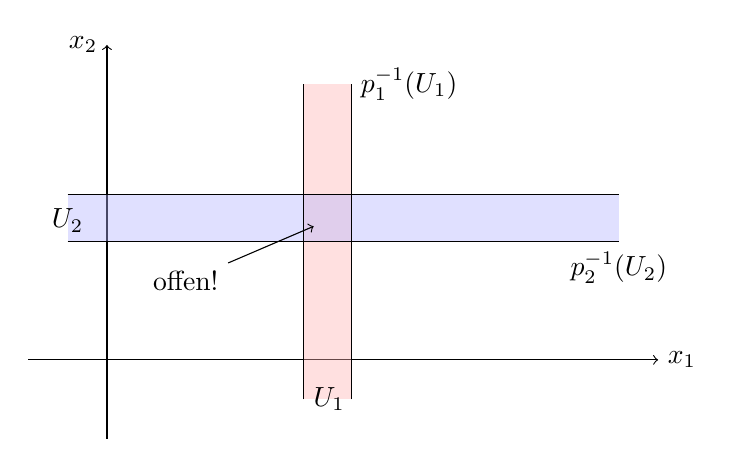
\begin{tikzpicture}
	%Achsen zeichnen
	\draw[->] (-1,0) -- (7,0) node[right] {$x_1$};
	\draw[->] (0,-1) -- (0,4) node[left] {$x_2$};
	%Rechtecke (die fuellung) zeichnen
	\fill[red!30, opacity=0.4] (2.5,-0.5) rectangle (3.1,3.5);
	\fill[blue!30, opacity=0.4] (-0.5,1.5) rectangle (6.5,2.1);
	%Balkenbegrenzungen zeichnen
	\draw (-0.5,1.5) node[above] {$U_2$} --(6.5,1.5) node[below] {$p_2^{-1}(U_2)$};
	\draw (-0.5,2.1) --(6.5,2.1);
	\draw (2.5,-0.5) node[right] {$U_1$}--(2.5,3.5);
	\draw (3.1,-0.5) --(3.1,3.5) node[right]{$p_1^{-1}(U_1)$};
	% "offen!" Beschriftung
	\node (o) at(1,1) {offen!}  node (p) at (2.75,1.75){ };
	\draw[->] (o) -- (p);
\end{tikzpicture}\end{center}
\end{enumerate}\end{DefErinn}

\begin{Frag}
Ist die Zariski-Topologie auf $k^2$ die Produkttopologie auf $\A ^1(k) \times \A ^1(k)$?
\end{Frag}

\newpage

%-------------------------- Abschnitt 4 --------------------------

\section{Irreduzible Komponenten}

\begin{DefBem}
Sei $X$ ein topologischer Raum.\begin{enumerate}[a)]
\item
	$X$ hei\ss t \defterm{reduzibel}, wenn es abgeschlossene Teilmengen $A, B \subseteq X$ gibt mit $A \cup B = X$ und $A\not= X\not= B$.  Eine Teilmenge von X heißt irreduzibel, wenn sie mit der induzierten Topologie irreduzibel ist.
\item
	Eine (bez\"uglich Inklusion) maximale irreduzibel Teilmenge von $X$ hei\ss t \deftermspec{irreduzible Komponente}{Komponente!irreduzible-}\index{irreduzibel!-Komponente} von $X$
\item
	Irreduzible Komponenten sind abgeschlossen (\"Ubung)
\end{enumerate}\end{DefBem}

\begin{Bsp}
Sei $X$ nichtleerer Hausdorffraum. Dann sind die einelementigen Teilmengen die irreduziblen Komponenten.

\emph{Denn:} Sei $X$ hausdorffsch, $x\not= y \in X$, \emph{zeige:} $X$ ist irreduzibel

Seien $U_x, U_y$ offene Umgebungen von $x$ bzw. $y$ mit $U_x \cap U_y = \emptyset$
\[\Rightarrow V_x \cup V_y = X, V_x = X-U_x, V_y = X- U_y\]
\[x\notin V_x \not= X \not=V_y \not\ni y\]
\end{Bsp}

\begin{Bsp}
$\A ^1(k)$ ist irreduzibel, wenn $k$ unendlich ist. \emph{Denn:} echte abgeschlossene Teilmengen von $\A ^1(k)$ sind endlich.
\end{Bsp}

\begin{Frag}
Ist $\A ^2(k)$ irreduzibel? Sei $\A ^2(k)=V_1 \cup V_2, V_i=V(I)$. Seien $f_1, f_2 \in I_1$ bzw. $I_2, f_i \not= 0$. $\Rightarrow V_i \subset V(f_i), i = 1,2$
\[\Rightarrow \underbrace{V(f_1)\cup V(f_2)}_{=V(f_1\cdot f_2)} = \A ^2\]
\begin{tikzpicture}
	%Achsen zeichen
	\draw[->] (-2,0) --(5,0);
	\draw[->] (0,-2) --(0,2);
	%Linie zeichnen
	\draw (-1.5,-1.5) --(1,1) node[right]{$f(X,0)$};
	\node(f) at (5,0.5){$f= f(X,Y)\in k[X,Y]$};
\end{tikzpicture}\\
$V(f)\cup V(Y) = V(f(X,0)) \subset \A ^1(k)$

Entweder $V(f(X,0))$ ist endlich \emph{oder} $f(X,0)=0$, dann ist durch $Y$ teilbar.
\linetitle{Genauso:} $f$ ist durch $Y-\alpha X$ teilbar f\"ur jedes $\alpha \in k \Rightarrow f=0$.
\linetitle{Antwort auf die Frage:} ja!
\end{Frag}

\begin{Prop}\label{4.4}
Eine affine Variet\"at $V\subseteq \A ^n(k)$ ist genau dann irreduzibel, wenn $I(V)$ ein Primideal ist.
\end{Prop}

\begin{Bew}\begin{twosidedproof}
\proofforward
	Seien $f,g\in k[X_1,\dots ,X_n]$ mit $f\cdot g \in I(V)$. Sei $f\notin I(V)$, zu zeigen: $g\in I(V)$
	
	$f\notin I(V) \Rightarrow \exists x\in V$ mit $f(x) \not= 0$
	
	Nach Voraussetzung ist $V\subseteq V(f\cdot g) = V(f)\cup V(g)$
		\[\Rightarrow V=\left(V(f)\cap V\right) \cup \left(V(g)\cap V\right) \stackrel{V \textrm{ irred.}}\Rightarrow V(g)\cap V = V\]
	$\Rightarrow V\subseteq V(g) \Rightarrow g\in I(V)$
\proofreverse
	Sei $I(V)$ Primideal, $V=V_1\cup V_2$ mit abgeschlossenen Teilmengen $V_1,V_2$, also $V_i=V(I_i), i=1,2$, f\"ur Ideale $I_1,I_2$. Sei $V\not= V_1$, also $V\subsetneq V(I_1)$.
		\[\Rightarrow \exists x\in V, f\in I_1 \textrm{ mit } f(x) \neq 0 \Rightarrow f\notin I(V)\]
	Wegen $V= V_1 \cup V_2=V(I_1)\cup V(I_2) \stackrel{\autoref{bem3.1}}=V(I_1\cdot I_2)$ ist $I_1\cdot I_2 \subseteq I(V)$ $\Rightarrow f\cdot g \in I(V)$ f\"ur jedes $g\in I_2$
		\[\overset{f\notin I(V)}{\underset{I(V) \textrm{ prim}}{\Rightarrow}} g \in I(V) \textrm{ f"ur jedes }g \in I_2\]
	$\Rightarrow I_2\subseteq I(V) \Rightarrow \underbrace{V(I_2)}_{=V_2} \supseteq \underbrace{V(I(V))}_{=V}$
\end{twosidedproof}\end{Bew}

\begin{Folg}
Eine affine Variet\"at$V\subset \A ^n(k)$ ist irreduzibel $\Leftrightarrow A(V) =k[X_1,\dots X_n]/I(V)$ ist nullteilerfrei.
\end{Folg}

\begin{Satz}
Sei $V\subseteq \A ^n(k)$ affine Variet\"at. Dann gilt:\begin{enumerate}[a)]
\item
	$V$ ist endliche Vereinigung von irreduziblen affinen Variet\"aten.
\item
	$V$ hat nur endlich viele irreduzible Komponenten, diese sind eindeutig bestimmt.
\end{enumerate}\end{Satz}

\begin{Bew}\begin{enumerate}[a)]
\item
	Sei $\calB=\{V\subseteq \A ^n(k)$ affine Variet\"at, $V$ ist \emph{nicht} endliche Vereinigung von irreduziblen affinen Variet\"aten$\}$
		\[\calI =\{I(V) : V\in \calB\}\]
	\emph{zu zeigen:} $\calB = \emptyset$, also auch $\calI = \emptyset$
	
	W\"are $\calI \neq \emptyset$, so enthielte $\calI$ ein maximales Element $I_0=I(V_0)$ f\"ur ein $V_0\in \calB$. (\emph{denn:} $k[X_1,\dots ,X_n]$ ist noethersch, jede aufsteigende Kette von Elementen in $\calI$ wird also station\"ar.) Da $V_0\in \calB$ ist $V_0$ reduzibel.
	
	Sei also $V_0=V_1\cup V_2$ mit abgeschlossenen Teilmengen $V_1\neq V_0 \neq V_2$ von $V_0$. Aus $V_i\subsetneq V_0$ folgt $I(V_i)\supsetneq\underbrace{I(V_0)}_{=I_0}$ (Bem. \ref{bem2.4} \ref{bem2.4.iv}))
		\[\Rightarrow I(V_i)\notin \calI \Rightarrow V_i\notin \calB, i=1,2\]
	$\Rightarrow V_i$ ist endliche Vereinigung von irreduziblen Variet\"aten, also auch $V_0 \notin \calB \lightning$
\item
	Sei $V=V_1,\dots ,V_r$ mit irreduziblen Variet\"aten $V_1,\dots ,V_r$. \OE $V_i\nsubseteq V_j$ f\"ur $i\neq j$ (sonst lasse $V_i$ weg)
	
	\textbf{Behauptung:} Dann ist jedes $V_i$ irreduzible Komponente.
	
	\emph{denn:} Sei $W \subseteq V$ irreduzible Komponente mit $V_i\subseteq W$. Es gilt
		\[W = \bigcup_{j=1}^r (V_i \cap W)\]
	$\overset{W \textrm{ irred.}}{\Longrightarrow} \exists j$ mit $V_j \cap W=W$, also $W\subseteq V_j$ $\Rightarrow V_i\subseteq V_j \Rightarrow i=j\Rightarrow W=V_i$
	\begin{description}[\setlabelstyle{\itshape}]
	\item[Eindeutigkeit:] Sei $W$ irreduzible Komponente von $V$. Aus $W= \bigcup_{j=1}^r(V_j\cap W)$ folgt $W\cap V_j=W$ f\"ur ein $j$	$\Rightarrow W\subseteq V_j  \overset{W \textrm{ irred. Komp.}}{\Longrightarrow }W=V_j$
\end{description}\end{enumerate}\end{Bew}

\begin{Prop}
Die irreduzible Teilmenge eines topologischen Raumes $X$ ist enthalten in einer irreduziblen Komponente von $X$.
\end{Prop}

\newpage

%-------------------------- Abschnitt 5 --------------------------

\section{Der Hilbertsche Raum}

$V$ affine Variet\"at in $ \A ^n(k) \Rightarrow V(I(V))=V$; $I\subseteq k[X_1,\dots ,X_n]$ Ideal $\Rightarrow I(V(I))\supseteq I$

\begin{nnBsp}
$I=(X^2+1)\subset\R[X]$

$V(I)=\emptyset \Rightarrow I(V(I)) = \R[X]$
\end{nnBsp}

\begin{Satz}\label{satz3}
Sei $k$ algebraisch abgeschlossener K\"orper.\begin{enumerate}[a)]
\item\label{satz3a}
	Ist $I\subsetneq k[X_1,\dots ,X_n]$ Ideal, so ist $V(I)\not=\emptyset$.
\item
	F\"ur jedes Ideal $I\subseteq k[X_1,\dots ,X_n]$ gilt
		\[I(V(I)) = \sqrt I\]
\end{enumerate}\end{Satz}

Der Beweise benutzt

\begin{nnSatz3}\label{hilfsatz3}
Ist $k$ K\"orper, $n\ge1, m\subset k[X_1,\dots ,X_n]$ maximales Ideal, so ist $L:=k[X_1,\dots X_n]/m$ \emph{algebraische} K\"orpererweiterung von $k$. Das hei\ss t f\"ur jedes $\alpha\in L$ gibt es ein $f\in k[X]$ mit $f(\alpha)=0$, also gibt es $d\ge1$ und $b_0,\dots ,b_{d-1}\in k$ mit
	\[\alpha^d+b_{d-1}\alpha^{d-1}+\dots +b_1\alpha + b_0=0\]
$k(\alpha):=k[X]/(f)$ ist K\"orper, der kleinste Teilk\"orper von $L$, der $k$ und $\alpha$ enth\"alt.
\end{nnSatz3}

\begin{Folg}\label{folg5.1}
Ist $k$ algebraisch abgeschlossen, so gibt es Bijektion zwischen den Mengen der\begin{enumerate}[i)]
\item
	Punke $x=(x_1,\dots ,x_n)$ in $k^n$
\item
	Ideale $m_x=(X_1-x_1,\dots ,X_n-x_n)$ in $k[X_1,\dots ,X_n]$
\item
	maximalen Ideale in $k[X_1,\dots ,X_n]$
\end{enumerate}\end{Folg}

\begin{Bew}\begin{enumerate}[(iii)]
\item[(i)$\to$(ii)] $\checkmark$

\item[(ii)$\to$(iii)]
	$m_x$ ist maximales Ideal. Die Abbildung $\varphi_x:k[X_1,\dots ,X_n]\to k, X_i\mapsto x_i, f\mapsto f(x)$ ist der Einsetzungshomomorphismus. $\Kern(\varphi_x)=m_x$

\item[(iii)$\to$(i)]
	Sei $m$ maximales Ideal, $\varphi:k[X_1,\dots ,X_n]\to k[X_1,\dots ,X_n]/m  \xrightarrow[\textrm{Satz 3'}]{\sim} k \Rightarrow m=\Kern(\varphi)$
	
	Sei $x_i=\varphi(X_i)$, dann ist $\varphi=\varphi_x$ f\"ur $x=(x_1,\dots ,x_n) \Rightarrow m=m_x$
\end{enumerate}\end{Bew}

\begin{Bew}[Beweis von Satz 3]\begin{enumerate}[a)]
\item
	Sei $I\subsetneq k[X_1,\dots ,X_n]$ echtes Ideal. Sei $m$ maximales Ideal mit $I\subseteq m$ (gibt es !) $\Rightarrow V(I) \supseteq V(m) \neq \emptyset$, da $m=m_x$ f\"ur ein $x\in k^n$ und $\{x\}=V(m_x)$
	
	\begin{Bew}[von Satz 3']
	Sei $x_i\in L$ die Restklasse von $X_i$. \emph{Zu zeigen:} $x_1,\dots ,x_n$ sind algebraisch \"uber $k$.
	
	\emph{Induktion \"uber $n$:} $n$=1, $m=(f)$ f\"ur ein irreduzibles Polynom $f \Rightarrow L=k[X]/(f)$ ist $k$-Verktorraum der Dimension $d= \deg(f)$
	
	Sei $n\geq 2$: \emph{Annahme:} $x_1$ ist transzendent.
	
	Dann ist $k'=k(x_1) \cong \underbrace{k(X_1)}_{=\Quot{(k[X_1])}}$ Teilk\"orpererweiterung von L. L wird \"uber $k'$ von $x_2,\dots ,x_n$ erzeugt $\Rightarrow L \cong k'[X_2,\dots ,X_n]/m'$ f\"ur ein maximales Ideal $m'$ in $k'[X_2,\dots ,X_n]$
	
	Nach Induktionsvoraussetzung ist $L$ algebraisch \"uber $k'$, das hei\ss t:
	\[\begin{array}{rclccrl}
		x_i^{d_i} + \sum\limits_{j=0}^{d_i-1} a_{ij}x_i^j &=& 0 & \quad & i=2,\dots ,n, d_i \geq1 & a_{ij} &\in k'\\
		a_{ij} &=& \frac{c_{ij}}{b_{ij}} & \quad & & b_{ij}, c_{ij} &\in k[X_1]
	\end{array}\]
	\end{Bew}

	\begin{enumerate}[(1)]
	\item Sei $R\subset k'$ die von den $a_{ij}$ erzeugte $k$-Algebra.
	\item Dann sind $x_1,\dots ,x_n$ ganz \"uber $R$ $\Rightarrow L$ ist ganze Ringerweiterung von $R$
	\item $\Rightarrow R=k$ oder $R$ ist kein K\"orper.
	\begin{enumerate}[(1)]
	\item $\Rightarrow R=k$ oder $R$ ist kein K\"orper.
	
		$R=k \Rightarrow $ f\"ur $\tilde k=k(x_2,\dots ,x_n)$ ist $L= \tilde k[X_1]/m$, also algebraisch abgeschlossen.
		
		$R\neq k \Rightarrow k(X_1)$ ist nicht endlich erzeugbar als $k$-Algebra.
	\item $\Rightarrow R$ ist K\"orper: Sei $a\in R\backslash\{0\}$. In $L$ gibt es $\frac{1}{a}$
		\[\Rightarrow \left(\frac{1}{a}\right)^d+\sum_{j=0}^{d-1} b_j\left(\frac{1}{a} \right)^j\textrm{ f\"ur ein } d\geq1, b_j\in R\]
		\[\Rightarrow 1+\sum_{j=0}^{d-1} b_ja^{d-j} = 0, 1 = a\left( -\sum_{j=0}^{d-1}b_ja^{d-1-j} \right)\]
	\end{enumerate}\end{enumerate}
	
\item
Sei $I\subseteq k[X_1,\dots ,X_n], g\in I(V(I))$.

\emph{Zu zeigen:}  es gibt $d\geq 0$ mit $g^d\in I$.

W\"ahle Erzeuger $f_1,\dots , f_n$ von $I$ (geht nach Satz \ref{satz1}). Betrachte in $k[X_1,\dots ,X_n,Y]$ das von $f_1,\dots ,f_n$ und $g\cdot Y-1$ erzeugte Ideal $J$.

\emph{Behauptung:} $V(J) = \emptyset$

\emph{denn:} Sei $x= (x_1,\dots ,x_n, y) \in V(J)$

Dann ist $f_i(x)= 0$ f\"ur $i=1,\dots ,m$. $\Rightarrow $ f\"ur $x'=(x_1,\dots ,x_n)$ ist $f_i(x')=0 \Rightarrow x'\in V(I)$ $\Rightarrow g(x')=0 \Rightarrow g(x)=0\Rightarrow (gY-1)(x)=g(x)\cdot y-1 = -1 \not=0$

Dann ist nach Satz \ref{satz3} \ref{satz3a}) $J=k[X_1,\dots ,X_n,Y]$
	\[\Rightarrow 1= \sum_{i=1}^m b_i f_i + b(gY-1) \textrm{ f\"ur geeignete }b_i, b\in k[X_1,\dots ,X_n,Y]\]
Sei $R =k[X_1,\dots ,X_n,Y]/(gY-1)$
	\[\Rightarrow 1=\sum_{i=1}^m \bar{b}_if_i \textrm{ f\"ur }\bar{b}_i = b_i \modmodulo(gY-1)\]
\emph{Es gilt:} \[R\cong k[X_1,\dots ,X_n][\frac{1}{g}]\]
	\[\bar b_i= \frac{a_i}{g^{d_i}}, a_i\in k[X_1,\dots ,X_n], d_i \geq0\]
$\Rightarrow$ F\"ur $d= \max d_i$ gilt
	\[g^d = \sum_{i=1}^n \underbrace{\left( g^d \bar b_i \right)}_{\in k[X_1,\dots ,X_n]} \cdot f_i \in I\]
\end{enumerate}\end{Bew}

% Vorlesung vom 2.11.
\begin{Folg}
Sei $k$ algebraisch abgeschlossen, $n\geq 1$,
	\[\begin{array}{rl}\calV_n := & \{V\subseteq k^n : V \textrm{ affine Variet\"at}\}\\
	\calI_n := & \{ I\subseteq k[X_1,\dots ,X_n] : I \textrm{ Radikalideal}\} \end{array}\]
Dann sind \[\begin{array}{rll}
	I: & \calV_n \to \calI_n, & V \mapsto I(V)\\
	V: & \calI_n \to \calV_n, & I \mapsto V(I)\end{array}\]
bijektiv und zueinander invers.
\end{Folg}

\begin{Bem}
Sei $k$ algebraisch abgeschlossen, $V\subseteq \A ^n(k)$ affine Variet\"at. Dann entsprechen die Punkte in $V$ bijektiv den maximalen Idealen in
	\[ k(V) =A(V):= k[X_1,\dots ,X_n]/I(V) \]
\end{Bem}

\begin{Bew}
Die maximalen Ideale in $A(V)$ entsprechen bijektiv den maximalen Idealen in $k[X_1,\dots ,X_n]$, die $I(V)$ enthalten, also (Folgerung \ref{folg5.1}) den Punkten in $k^n$, die in $V$ liegen.
\end{Bew}

$x= (x_1,\dots ,x_n), m_x=(X_1-x_1,\dots ,X_n-x_n)=I(\{x\})$

$I(V) \subseteq I(\{x\})$

$V = V(I(V)) \supseteq V(I(\{x\})) = \{x\}$

\newpage

%-------------------------- Abschnitt 6 --------------------------

\section{Morphismen affiner Variet\"aten}

\begin{DefBem} \label{6.1}
Sei $k$ ein K\"orper, $V\subseteq \A ^n(k)$, $W\subseteq \A ^m(k)$ affine Variet\"aten.\begin{enumerate}[a)]
\item
	Eine Abbildung $f: V \to W$ hei\ss t \defterm{Morphismus}, wenn es Polynome $f_1,\dots ,f_m \in k[X_1,\dots ,X_n]$ gibt mit
		\[f(x) = (f_1(x),\dots ,f_n(x))\]
	f\"ur alle $x\in V$.
\item
	Ein Morphismus $f: V\to W$ hei\ss t \deftermspec{Isomorphismus}{Morphismus!Iso-}, wenn es einen Morphismus $g:W\to V$ gibt mit
		\[ g\circ f = \id_W \textrm{ und } f\circ g = \id_V\]
\item
	Die affinen Variet\"aten \"uber $k$ bilden mit den Morphismen aus a) eine Kategorie $\Aff(k)$.
	
\item\label{bem6.1d}
	Jeder Morphismus $f:V\to W$ ist Einschr\"ankung eines Morphismus $\tilde f: \A ^n(k) \to \A ^m(k)$
\end{enumerate}\end{DefBem}

\begin{Bsp}\begin{enumerate}[1)]
\item\begin{enumerate}[$\bullet$]
	\item[$\bullet$] Einbettungen \[\begin{array}{rcl}\A^n(k) &\to& \A ^m(k) (n\leq m)\\
		(x_1,\dots ,x_n) & \mapsto & (x_1,\dots ,x_n,0,\dots ,0)\end{array}\]
	\item[$\bullet$] Projektionen \[\begin{array}{rcl}\A^n(k) &\to& \A ^m(k) (n\geq m)\\
		(x_1,\dots ,x_n) & \mapsto & (x_1,\dots ,x_m) \end{array} \]
	\item[$\bullet$] Permutation der Komponenten \[\begin{array}{rcl}
		(x_1,\dots ,x_n) & \mapsto & (x_{\sigma(1)},\dots ,x_{\sigma(n)}) \end{array} \]
	\end{enumerate}
\item
	Jedes $f\in k[X_1,\dots ,X_n]$ definert einen Morphismus
		\[f:\A ^n(k) \to A^1(k), x\mapsto f(x)\]
\item
	Sei $V=\A ^1(k)$, $W =V(Y^2 - X^3)\subseteq \A ^2(k)$.
	
	$f:V\to W$, $x\mapsto (x^2,x^3)$ ist Morphismus. $f$ ist bijektiv mit Umkehrabbildung\[
		g(x,y)=\left\{\begin{array}{lcl}
			0 & \quad & \textrm{ falls } (x,y)=(0,0)\\
			\frac{y}{x} & \quad & \textrm{ falls } (x,y)\not= (0,0) \end{array}\right.\]
	$g(f(x))=g(x^2,x^3) = \frac{x^3}{x^2}=x$ (f\"ur $x\not= 0$)
	
	$f(g(x,y))=f(\frac{y}{x})=(\frac{y^2}{x^2}, \frac{y^3}{x^3})=(\frac{x^3}{x^2}, \frac{y^3}{y^2})$
	
	Ist $k$ unendlich, so ist $g$ kein Morphismus!
\item
	Sei $\chara (k) = p > 0$ \[
		f: \A ^n(k) \to \A ^n(k), (x_1,\dots ,x_n)\mapsto (x_1^p,\dots ,x_n^p)\]
	hei\ss t \deftermspec{Frobenius-Homomorphismus}{Morphismus!Homo-!Frobenius-}.
	
	Die Fixpunkte von $f$ sind genau die Punkte, deren Koordninaten alle in $\F_p$ liegen (\quot{$\F_p$-wertige Punkte})
		\[\left( a^p=a \Leftrightarrow a \textrm{ Nullstelle von } X^p-X \Leftrightarrow a\in \F_p \right) \]
\end{enumerate}\end{Bsp}

\begin{Bem}\label{bem6.3}
Morphismen affiner Variet\"aten sind stetig bez\"uglich der Zariski-Topologie.
\end{Bem}

\begin{Bew}
Seien $V\subseteq \A ^n(k)$, $W\subseteq \A ^m(k)$ affine Variet\"aten, $f:V\to W$ Morphismus. Sei $Z\subseteq W$ abgeschlossen, also $Z=V(J)$ f\"ur ein Ideal $J\subseteq k[X_1,\dots ,X_n]$. Sei $I=\{g\circ f\in k[X_1,\dots ,X_n]:g\in J\}$.\\
\emph{Behauptung:} $V(I)=f^{-1}(Z)$\\
\emph{denn:}
	\[x\in f^{-1}(Z) \Leftrightarrow f(x)\in Z \Leftrightarrow f(x)\in V(J) \Leftrightarrow g(f(x)) = 0 \forall g\in J \Leftrightarrow x\in V(I)\]
\end{Bew}

\begin{DefBem}
Sei $V\subseteq\A^n(k)$ affine Variet\"at.\begin{enumerate}[a)]
\item
	$k[V]:=\{f:V\to \A^1(k) : f \textrm{ ist Morphismus}\}$ hei\ss t \deftermspec{affiner Koordinatenring}{Ring!affiner Koordinaten-} von V.
\item
	\[k[V] \cong A(V)=k[X_1,\dots ,X_n]/I(V)\]
\end{enumerate}\end{DefBem}

\begin{Bew}\begin{enumerate}[b)]\item
Sei $\varphi:k[X_1,\dots ,X_n]\to k[V], f\mapsto f_{\vert V}$ Einschr\"ankungshomomorphismus. $\varphi$ ist surjektiv (Bemerkung \ref{6.1} \ref{bem6.1d}))

$\Kern(\varphi)=I(V) \overset{\textrm{Homomorphiesatz}}{\Longrightarrow}$ Behauptung
\end{enumerate}\end{Bew}

\begin{Prop}
Seien $V\subseteq\A^n(k), W\subseteq\A^m(k)$ affine Variet\"at.\begin{enumerate}[a)]
\item
	Jeder Morphismus $\varphi = f:V\to W$ induziert $k$-Algebrahomomorphismus \[f^{\#}:k[W]\to k[V], g\mapsto g\circ f\]
\item
	Die Abbildung $\Mor(V,W)\to \Hom_k(k[W],k[V]), f\mapsto f^{\#}$ ist bijektiv.
\end{enumerate}\end{Prop}

\begin{Bew}\begin{enumerate}[a)]
\item $\checkmark$ \item\begin{description}[\setlabelstyle{\itshape}]
	\item[injektiv:]
		Seien $f,\tilde f:V\to W$ Morphismen mit $f^{\#}=\tilde f^{\#}$
		
		$\Rightarrow g\circ f=g\circ\tilde f$ f\"ur alle$g\in k[W]$
		
		Insbesondere ist $\underbrace{p_i\circ f}_{=f_i}=\underbrace{p_i\circ\tilde f}_{=\tilde f_i}$ f\"ur die Projektion
			\[p_i:W\to \A^1(k), (x_1,\dots ,x_n)\mapsto x_i\]
		$\Rightarrow f=\tilde f$
	\item[surjektiv:] Sei $\varphi : k[W]\to k[V]$ $k$-Algebra-Homomorphismus.
		
		Definiere $f:V\to\A^m(k)$ durch $f(x)=(\varphi(p_1)(x),\dots ,\varphi(p_n)(x))$
		
		\emph{Behauptung:}\begin{enumerate}[(i)]
		\item $f^{\#}=\varphi$
		\item $f(V)\subseteq W$\end{enumerate}
		Zu (i): f\"ur $i=1,\dots ,m$ gilt:
			\[f^{\#}(p_i)=p_i\circ f = \varphi(p_i)\]
		Da die $p_i$ $k[V]$ erzeugen (als $k$-Algebra), folgt $f^{\#} = \varphi$
		
		Zu (ii): Sei $g\in I(W), x\in V$
		
		Zu zeigen: $g(f(x))=0$
		\begin{center} 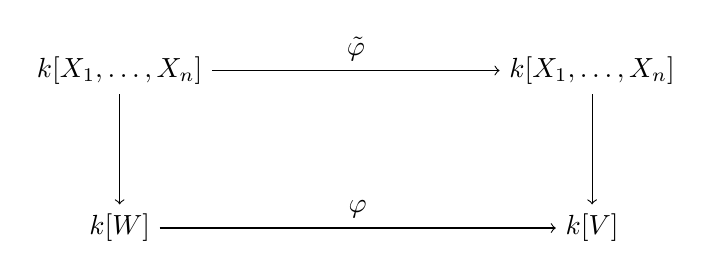
\begin{tikzpicture}
			%definierte die Punkte
		 	\node (kx1) at (-3,1) {$k[X_1,\dots ,X_n]$} node (kx2) at (3,1) {$k[X_1,\dots ,X_n]$};
			\node (kw) at (-3,-1) {$k[W]$} node (kv) at (3,-1) {$k[V]$};
			%zeichne die Pfeile
			\draw[->] (kx1) -- node[above]{$\tilde{\varphi}$} (kx2);
			\draw[->] (kx1) -- (kw);
			\draw[->] (kw) -- node[above]{$\varphi$}(kv);
			\draw[->] (kx2) -- (kv);
		\end{tikzpicture} \end{center}
Lifte $\varphi$ zu $\tilde{\varphi}$. W\"ahle dazu f\"ur jedes $i$ ein Urbild von $\varphi(p_i)$. Dann ist $\tilde{\varphi}(I(W))\subseteq I(V)$ $\Rightarrow g(f(x))=g(\varphi(p_1)(x),\dots ,\varphi(p_m)(x)) = \tilde{\varphi}(g)(x)=0$
\end{description}\end{enumerate}\end{Bew}

% Vorlesung vom 7.11.
\begin{Bem}
Seien $V,W$ affine Variet\"aten \"uber $k$, $\varphi:k[W]\to k[V]$ $k$-Algebra-Homomorphismus und $f= f_{\varphi}: V\to W$ mit $f^{\#}=\varphi$. Dann gilt f\"ur jedes $x\in V$:
	\[ m_{f(x)}=\varphi^{-1}(m_x)\]
\end{Bem}

\begin{Bew}
$m_x=\{f\in k[V]: g(x)=0\}$
	\[\varphi^{-1}(m_x)=(f^{\#})^{-1}(m_x)=\{h\in k[W]:h\circ f \in m_x\} = \{h\in k[W]:h(f(x))=0\} =m_{f(x)}\]
\end{Bew}

\begin{Bsp}
$V = V(Y^2-X^3)\subseteq\A^2(k)$

$f: \A^1(k)\to V, x\mapsto(x^2,x^3)$
	\[f^{\#}:\underbrace{k[V]}_{=k[X,Y]/(Y^2-X^3)}\to k[\A^1(k)]=k[T]\]
$f^{\#}(\overline X)=T^2$

$f^{\#}(\overline Y)=T^3$

$f^{\#}$ ist injektiv, aber nicht nicht surjektiv! ($T\notin \Bild(f^{\#})$)

Es gilt aber: der von $f^{\#}$ auf dem Quotientenk\"orper induzierte Homomorphismus ist ein Isomorphismus $f^{\#}(\frac{Y}{X}) = T$.
\end{Bsp}

\begin{Satz}\label{satz4}\begin{enumerate}[a)]
\item
	Die Zuordnung $V\mapsto k[V]$ induziert einen volltreuen kontravarianten Funktor
		\[\Phi: \underline{\Aff(k)}\to \underline{k\textrm{-}\Alg^{\red}} \textrm{ (endl. erzeugte }k\textrm{-Alg.)}\]
\item
	Ist $k$ algebraisch abgeschlossen, so ist $\Phi$ eine \"Aquivalenz von Kategorien.
\end{enumerate}\end{Satz}

\begin{Bew}\begin{enumerate}[a)]\item $\checkmark$\item
Noch zu zeigen: zu jeder $k$-Algebra $A\in k\Alg^{\red}$ gibt es affine Variet\"at $V$ \"uber $k$ mit $k[V]\cong A$. $A$ werde als $k$-Algebra erzeugt von $a_1,\dots ,a_n$. Sei $\varphi: k[X_1,\dots ,X_n]\to A$ der durch $\varphi(X_i)=a_i$ definierte $k$-Algebra-Homomophismus. $\varphi$ ist surjektiv, da $A$ von den $a_i$ erzeugt wird.
	\[\Rightarrow A \cong k[X_1,\dots ,X_n]/\Kern(\varphi)\]
Sei $V=V(\Kern(\varphi))\Rightarrow I(V) \stackrel{\textrm{HNS}}{=} \sqrt{\Kern(\varphi)} = \Kern(\varphi)$ $\Rightarrow k[V]=k[X_1,\dots ,X_n]/I(V)\cong A$
\end{enumerate}\end{Bew}

\newpage

%-------------------------- Abschnitt 7 --------------------------


\section{Die Garbe der regul\"aren Funktionen}
Sei $k$ algebraisch abgeschlossener K\"orper

\begin{Bem}\label{bem7.1}
Sei $V\subset \A^n(k)$affine Variet\"at \"uber $k$, $h\in k[X_1,\dots ,X_n]$. Dann gilt: $\overline h$ ist Einheit in $k[V] \Leftrightarrow V(h)\cap V=\emptyset$
\end{Bem}

\begin{Bew}\[\begin{array}{rl}
V\cap V(h) &=V(I(V)+(h))=\emptyset \overset{\textrm{HNS}}{\Longleftrightarrow}I(V)+(h)=k[X_1,\dots ,X_n]\\
	&\Leftrightarrow 1=f+gh \textrm{ f\"ur gewisse } f\in I(V), g\in k[X_1,\dots ,X_n]\\
	&\Leftrightarrow \overline{1} = \overline g \cdot h \textrm{ in } k[V]
\end{array}\]\end{Bew}

\begin{DefBem}\label{Def7.2}
Sei $V\subseteq\A^n(k)$ affine Variet\"at, $U\subseteq V$ offen, $p\in U$.\begin{enumerate}[a)]
\item
	Eine Abbildung $f:U\to \A^1(k)$ hei\ss t \deftermspec{regul\"ar in p}{regul\"ar!in $p$}, wenn es eine Umgebung $U_p\subseteq U$ von $p$ gibt und $g,h\in k[V]$ mit $h(x)\neq 0$ f\"ur alle $x\in U_p$ und $f(x)=\frac{g(x)}{h(x)}$ f\"ur alle $x\in U_p$.
\item
	$f:U\to \A^1(k)$ hei\ss t \defterm{regul\"ar}, wenn $f$ in jedem $p\in  U$ regul\"ar ist.
\item
	$\calO(U):=\{f:U\to\A^1(k): f \textrm{ regul\"ar}\}$ hei\ss t $k$-Algebra (oder Ring) der \deftermspec{regul\"aren Funktionen}{regul\"ar!Funktionen} auf $U$.
\item
	F\"ur jedes offene $U\subseteq V$ ist
		\[\alpha_U : k[V]\to\calO_V(U), f\mapsto f_{|_U}\]
	ein $k$-Algebra-Homomophismus.
	
	\emph{Zusatz:} Ist $U$ dicht, so ist $\alpha_U$ injektiv (\"Ubung?)
\end{enumerate}\end{DefBem}

\begin{nnBsp}\begin{enumerate}[1)]
\item
	$V=\A^1(k), U=\A^1(k)-\{0\}, f(x) = \frac{1}{x}$
\item
	$V=V(Y^2-X^3)\subset\A^2(k), U=V-\{0,0\}$ $\Rightarrow g=\frac{y}{x}\in \calO_V(U)$
\item
	$f\in k[X_1,\dots ,,X_n] \Rightarrow \frac{1}{f}\in \calO_{\A^n(k)}(D(f))$
\end{enumerate}\end{nnBsp}

\begin{Bem}
Sei $V\subseteq\A^n(k)$ affine Variet\"at, $U\subseteq V$ offen.\begin{enumerate}[a)]
\item
	F\"ur offene Teilmengen $U''\subseteq U' \subseteq U$ gilt:
	\begin{itemize}
		\item[(i)] $\varrho_{U'}^{U}: \calO_V(U) \to \calO_V(U'), f \mapsto f_{|_{U'}}$ ist k-Algebra Homomorphismus
		\item[(ii)] $\varrho_{U''}^{U} = \varrho_{U''}^{U'} \circ \varrho_{U'}^{U}$
	\end{itemize}
\item
	Sei $(U_i)_{i \in I}$ offene Überdeckung von U (mit Indexmenge I).Dann gilt:
	\begin{itemize}
		\item[(i)] Für $f \in \calO_V(U)$ ist $ f=0 \Leftrightarrow f_{|_{U_i}}=0 \forall i \in I$
		\item[(ii)] F\"ur jedes $i\in I$ sei $f_i\in \calO_V(U_i)$ gegeben.
		
		Ist $f_{i\vert U_i \cap U_j} =f_{j\vert U_i \cap U_j}$ f\"ur alle $i,j$, so gibt es $f\in \calO_V(U)$ mit $f_{\vert U_i}=f_i$ f\"ur alle $i\in I$.
	\end{itemize}	
\end{enumerate}\end{Bem}

\begin{FolgDef}
Die Zuordnung $U\mapsto \calO_V(U)$ ist eine Garbe von Ringen auf dem topologischen Raum $V$.

Allgemeiner:\begin{enumerate}[a)]
\item
	ist \deftermspec{Pr\"agarbe}{Garbe!Pr\"a-}
\item
	ist die \deftermspec{Garbeneigenschaft}{Garbe!Garbeneigenschaft}
\end{enumerate}\end{FolgDef}

\begin{nnBsp}
$X$ topologisher Raum, $R$ ein Ring. F\"ur $U\subseteq X$ offen sei $\calF(U)=R, \varrho^U_{U'}=\id_R$. Ist $\calF$ Garbe? Pr\"agarbe: JA! Garbe nein, falls es disjunkte offene Mengen gibt!
\end{nnBsp}

%Vorlesung vom 9.11.
\begin{Bem}\label{7.5}\label{bem7.5}
Sei $V\subseteq \A^n(k)$ affine Variet\"at, $U\subseteq V$ offen.\begin{enumerate}[a)]
\item
	Jede absteigene Kette $V_1 \supseteq V_2 \supseteq \dots $ von abgeschlossenen Teilmengen von $V$ wird station\"ar (\quot{$V$ ist noetherscher topologischer Raum})
	
\item
	$U$ ist quasikompakt, das hei\ss t jede offene \"Uberdeckung von $U$ hat endliche Teil\"uberdeckung.
\end{enumerate}\end{Bem}

\begin{Bew}\begin{enumerate}[a)]
\item
$V_i=V(I_i)$, $I_i$ Ideal in $k[V]$

$V_i\supseteq V_{i+1} \Rightarrow I_{i+1} \supseteq I_i$

$k[V]$ ist noethersch $\Rightarrow $ Behauptung

\item\label{bem7.5b}
Sei $(U_i)_{i\in I}$ offene \"Uberdeckung von U.

Besitzt $(U_i)$ keine endliche Teil\"uberdeckung, so gibt es Folge $(U_{I_k})_{k=1,2,\dots }$ mit $U_{i_{k+1}} \nsubseteq \bigcup_{j=1}^k U_{i_j}.$

$W_k:= \bigcup_{j=1}^k U_{i_j}$ ist offen in $V \stackrel{a)}{\Rightarrow} (W_k)$ wird station\"ar.
\end{enumerate}\end{Bew}

\begin{Satz}\label{satz5}
Sei $V\subseteq\A^n(k)$ affine Variet\"at.\begin{enumerate}[a)]
\item\label{satz5a}
	$\calO_v(V) \cong k[V]$

\item\label{satz5b}
	$\calO_v(\underbrace{D(f)}_{=\A^n(k)\backslash V(f)}) \cong k[V]_f = k[f]_{\{f^d:d\ge 0\}}$
	f\"ur alle $f\in k[V]\backslash\{0\}$
\end{enumerate}\end{Satz}

\begin{Bew}\begin{enumerate}[a)]
\item Ist ein Spezielfall von b) f\"ur $f=1$.

\item
Definiere\[\begin{array}{rlr}
	\alpha:k[V]_f & \to \calO_V(D(f)) & \\
	\frac{g}{f^d} & \mapsto (x\mapsto \frac{g(x)}{f(x)^d}) &\quad (x\in D(f))\end{array}\]
\begin{description}[\setlabelstyle{\itshape}]
\item[$\alpha$ wohldefiniert:]
	Sei $\frac{g_1}{f^{d_1}} = \frac{g_2}{f^{d_2}}$ in $k[V]_f$
	
	$\Rightarrow f^d(g_1 \cdot f^{d_2} - g_2 \cdot f^{d_1}) = 0$ f\"ur ein $d\geq 0$
	
	f\"ur $x\in D(f)$ ist $g_1(x)f(x)^{d_2} -g_2(x)f(x)^{d_1}=0$
	
	$\Rightarrow  \frac{g_1(x)}{f(x)^{d_1}}= \frac{g_2(x)}{f(x)^{d_2}}$
\item[$\alpha$ injektiv:] Sei $\frac{g(x)}{f(x)^d}=0$ f\"ur alle $x\in D(f)$

	$\Rightarrow g(x) =0$ f\"ur alle $x\in V$
	
	$\Rightarrow f\cdot g=0$ in $k[V]$
	
	$\Rightarrow g=0$ in $k[V]_f$
\item[$\alpha$ surjektiv:] Sei $g\in \calO_V(D(f))$

	$\Rightarrow $ f\"ur jedes $p\in D(f)$ gibt es Umgebung $U_p\subseteq D(f)$ und $g_p,h_p \in k[V]$ mit $g(x) = \frac{g_p(x)}{h_p(x)} \forall x\in U_p$
	
	\emph{Behauptung 1:} \OE $U_p=D(h_p)$
	
	\emph{denn:} es gibt $\tilde h_p \in k[V]$ mit $D(\tilde h_p)\subseteq U_p(\subseteq D(h_p))$
	
	$\Rightarrow V(\tilde h_p)\supset V(h_p) \Rightarrow \tilde h_p\in I(V(h_p)) \stackrel{HNS}{=} \sqrt{(h_p)}$
	
	$\Rightarrow \exists d\geq 0, h\in k[V]$ mit $\tilde h_p^d =h\cdot h_p$
	
	Setze $\hat g_p = h g_p, \hat h = \tilde h_p^d = h\cdot h_p$
	
	Dann gilt f\"ur jedes $x\in D(\hat h_p)=D(\tilde h_p)$
		\[g(x)=\frac{g_p(x)}{h_p(x)}=\frac{g_p(x)\cdot h(x)}{h_p(x)\cdot h(x)}=\frac{\hat g_p(x)}{\hat h_p(x)}\]
	\autoref{7.5} $\Rightarrow D(f)=$ \fbox{$D(h_1)\cup \dots  \cup D(h_r)$} (1)
	f\"ur geeignete $h_i:=h_{p_i}, 1= 1,\dots ,r$
	
	Nach Behauptung 1 ist \OE $ g= \frac{g_i}{h_i}$ auf $D(h_i)$
	
	\emph{Behauptung 2:} $g_i h_j = g_j h_i$ in $k[V]$ f\"ur alle $i,j$
	
	\emph{denn:} es ist $g_ih_j = g_jh_i$ auf $D(h_i)\cap D(h_j)=D(h_ih_j)$
	
	$\Rightarrow h_ih_j(g_ih_j-g_jh_i)=0$ in $k[V]$ (*)
	
	setze $\tilde g_i = g_ih_i, \tilde h_i = h_i^2$. Dann wird aus (*)
		\[\tilde g_i \tilde h_j -\tilde g_j \tilde h_i =0\]
	(1) $\Rightarrow V(f) =\bigcup_{i=1}^r V(h_i) \Rightarrow f \in I(V(h_1,\dots ,h_r)) \stackrel{HNS}{\Rightarrow } f\in \sqrt{(h_1,\dots ,h_n)}$
	
	$\Rightarrow \exists d\geq 0, b_i\in k[V]$ mit $f^d=\sum_{i=1}^rb_ih_i$
	
	Setze $\tilde g := \sum_{i=1}^rb_ig_i\in k[V]$
	
	Dan gilt f\"ur alle $i=1,\dots ,r$ und alle $x\in D(h_j)$:
		\[g(x)=\frac{g_j(x)}{h_j(x)}=\frac{g_j(x)f(x)^d}{h_j(x)f(x)^d}=\frac{(g_j\sum_{i=1}^rb_ih_i)(x)}{(h_jf^d)(x)} \stackrel{\textrm{Beh. 2}}{=} \frac{h_j(\sum_{i=1}^rb_ig_i)}{h_jf^d}(x) = \frac{\tilde g(x)}{f(x)^d}\]
\end{description}
\end{enumerate}\end{Bew}

\begin{Prop}
Seien $V\subseteq\A^n(k), W\subseteq \A^m(k)$ affine Variet\"aten. Dann gilt: $f:V\to W$ ist Morphismus $\Leftrightarrow$ $f$ stetig und f\"ur jedes offene $U\subseteq W$ und jedes $g\in \calO_W(U)$ ist $g\circ f\in \calO_V(f^{-1}(U))$
\end{Prop}

\begin{Bew}\begin{twosidedproof}
\proofforward
	$f$ stetig nach Bemerkung \ref{bem6.3}. Sei $g\in \calO_W(U), p \in f^{-1}(U)$. In einer Umgebung $U'$ von $p'=f(p)$ ist $g(y)=\frac{g_{p'}(y)}{h_{p'}(y)}$ f\"ur geeignete $g_{p'}, h_{p'}\in k[W]$.	F\"ur $x\in f^{-1}(U')$ ist also $g(f(x))=\frac{g_{p'}(f(x))}{h_{p'}(f(x))}$. Dabei ist\[\begin{array}{lcr}
		g_p'\circ f & = & f^{\#}(g_p')\in k[V]\\
		h_p'\circ f & = & f^{\#}(h_p')\in k[V]\end{array}\]
\proofreverse
	Zu zeigen: f\"ur $i=1,\dots ,m$ ist $p_i\circ f$ ein Polynom, wobei $p_i\in k[W]$ die Restklasse von $X_i$ ist.
	
	Nach Satz \ref{satz5} \ref{satz5a}) ist $k[W] = \calO_W(W)$ $\Rightarrow p_i\circ f\in \calO_V(V)=k[V]$
\end{twosidedproof}\end{Bew}

\begin{DefBem}\label{bem7.7}\begin{enumerate}[a)]
\item
	Eine Teilmenge $U\subseteq \A^n(k)$ hei\ss t \deftermspec{quasi-affine Variet\"at}{Variet\"at!affine-!quasi-}, wenn $U$ Zariski-offen in einer affinen Variet\"at $V$ ist.
\item
	Eine Abbildung $f: U_1 \to U_2$ zwischen quasi-affinen Variet\"aten $U_1,U_2$ hei\ss t \defterm{Morphismus} (oder \deftermspec{regul\"are Abbildung}{Abbildung!regul\"are-}), wenn $f$ stetig ist und f\"ur jedes offene $U \subseteq U_2$ und jedes $g\in\calO_{U_2}(U)$ gilt:
		\[g\circ f \in \calO_{U_1}(f^{-1}(U))\]
	(hier sei $\calO_{U_2}:=\calO_{\bar{U}_2}$, $\bar U_2$ der Z-Abschluss von $U_2$)	
\item
	$f:\overbrace{U_1}^{\subseteq\A^n(k)}\to\overbrace{U_2}^{\subseteq\A^m(k)}$ ist genau dann regul\"ar, wenn es regul\"are Funktionen $f_1,\dots ,f_n$ auf $U_1$ gibt mit $f(x)=(f_1(x),\dots ,n_m(x))$ f\"ur alle $x\in U_1$
\item
	Die quasi-affinen Variet\"aten \"uber $k$ bilden eine Kategorie, die $\underline{\Aff(k)}$ als volle Unterkategorie enth\"alt.
\item
	Eine quasi-affine Variet\"at hei\ss t \defterm{affin} (als abstrakte Variet\"at), wenn sie isomorph ist zu einer affinen Variet\"at.
\end{enumerate}\end{DefBem}

\begin{Bem}\label{bem7.8}
F\"ur $f\in k[X_1,\dots ,X_n]$ ist $D(f)$ (abstrakt) affin.

\linetitle{Beispiel:} $n=1, f(x)=x, D(f) =\A^1(k)-\{0\}$

\begin{minipage}[c]{0.5\linewidth}
	$V=V(XY-1)\subseteq\A^2(k)$
	
	$\varphi:V\to\A^1(k)$
	
	$(x,y)\mapsto x$
	
	$\Psi:\A^1(k)-\{0\}\to V,x\mapsto(x,\frac{1}{x})$
\end{minipage}
\begin{minipage}[c]{0.5\linewidth}\begin{tikzpicture}[scale=1]
	%Achsen zeichnen
	\draw[->] (-5,0) -- (5,0);%X-Achse
	\draw[->] (0,-4) -- (0,4);%Y-Achse
	%Funktion zeichnen (in zwei Abschnitten um nicht durch 0 zu teilen)
	\draw[ultra thick] plot[domain=-4:-0.3] (\x,{pow(\x,-1)});
	\draw[ultra thick] plot[domain=0.3:4] (\x,{pow(\x,-1)});
	%Die Dinger an der X-Achse
	\draw[ultra thick](-4.8,0) -- (-0.1,0);
	\draw[ultra thick](-0.4,0.3)--(-0.1,0.3)--(-0.1,-0.3)--(-0.4,-0.3);
	\draw[ultra thick](0.1,0) -- (4.8,0);
	\draw[ultra thick](0.4,0.3)--(0.1,0.3)--(0.1,-0.3)--(0.4,-0.3);
\end{tikzpicture}\end{minipage}
\end{Bem}

\begin{Bew}
Sei $g=f\cdot X_{n+1}-1\in k[X_1,\dots ,X_{n-1}]$ und $V=V(g)\subseteq\A^{n+1}(k)$, $V$ ist affine Variet\"at, $\varphi:D(f) \to V, x\mapsto(x,\frac{1}{f(x)})$ ist Morphismus mit Umkehrabbildung $\Psi: V(g) \to D(f), (x_1,\dots,x_(n+1))\mapsto (x_1,\dots,x_n)$.
\end{Bew}

\newpage

%-------------------------- Abschnitt 8 --------------------------
\section{Rational Abbildungen und Funktionenk\"orper}

$k$ sei wieder algebraisch abgeschlossen

\begin{DefBem}\label{bem8.1}
 Sei $V\subseteq\mathbb A^n(k)$ (quasi-)affine Variet\"at.\begin{enumerate}[a)]
\item
	Eine \deftermspec{rationale Funktion}{Funktion!rationale} auf $V$ ist eine \"Aquivalenzklasse von Paaren $(U,f)$, 
	wobei $U\subseteq V$ offen und dicht und $f\in\calO(U)$ ist. Dabei ist $(U,f)\sim(U',f'):\Leftrightarrow f|_{U\cap U'}=f'|_{U\cap U'}$
\item In jeder \"Aquivalenzklasse gibt es ein maximales Element $(U_{\max},f_{\max}), U_{\max}=:\Ddef(f)$ hei\ss t \defterm{Definitionsbereich} der nat\"urlichen Funktion. $V \setminus \Ddef(V)$ hei\ss t \defterm{Polstellenmenge} der rationalen Funktion.
\item
	Die rationalen Funktionen auf $V$ bilden eine $k$-Algebra $\Rat(V)$.
\item\label{bem8.1d}
	Ist $V$ irreduzibel, so ist $\Rat(V)= \Quot(k[V])=:k(V)$. $k(V)$ hei\ss t \deftermspec{Funktionenk\"orper}{Funktion!Funktionenk\"orper}.
\end{enumerate}\end{DefBem}

\begin{Bew}\begin{enumerate}[a)]
\item
	$\sim$ ist transitiv: Sei $(U_1,f_1)\sim(U_2,f_2), (U_2,f_2)\sim(U_3,f_3) \Rightarrow f_1|_{U_1\cap U_2\cap U_3}=f_3|_{U_1\cap U_2\cap U_3}$
	
	$U_1\cap U_2 \cap U_3$ ist (offen und) \emph{dicht} in $V \Rightarrow f_1|_{U_1\cap U_3} = f_3|_{U_1\cap U_3}$ (\"U4, A5)
\item
	\[U_{\max}=\bigcup_{\substack{\exists\ f\in \calO_V(U)\\ \textrm{ mit} (U,f)\in \textrm{ Klasse}}} U\]
\item
	$f\pm g, f\cdot g$ sind auf $\Ddef(f)\cap\Ddef(g)$ regul\"ar
\item
	$V$ irreduzibel $\Leftrightarrow I(V)$ Primideal $\Leftrightarrow k[V]$ ist nullteilerfrei
	
	\emph{Definiere:}\[\begin{array}{rcl}
		\alpha:k(V) &\to& \Rat(V)\\
		\frac{g}{h} &\mapsto& (D(h),\frac{g}{h})\end{array}\]
	\begin{description}
	\item
		\emph{$\alpha$ ist wohldefiniert}, weil $D(h)$ dicht ($V$ irreduzibel)
	\item
		\emph{$\alpha$ ist injekiv}: $\checkmark$
	\item
		\emph{$\alpha$ ist surjektiv}: Sei $[(U,f)]\in\Rat(V)$, also $f\in \calO_V(U) \Rightarrow \exists \ U'\subseteq U$ offen, $g,h \in k[V]$ mit $f=\frac{g}{h}$ auf $U'$. $V$ irreduzibel, also $U'$ dicht $\Rightarrow (U, f)\sim(U',\frac{g}{h})\sim (D(h),\frac{g}{h})$
		$\Rightarrow \alpha(\frac{g}{h})=[(U,f)]$
	
\end{description}\end{enumerate}\end{Bew}

\begin{DefBem}\label{bem7.2}
Seien $V,W$ affine Variet\"aten.\begin{enumerate}[a)]
\item
	Eine \deftermspec{rationale Abbildung}{Abbildung!rationale-} $f:V\dashrightarrow W$ ist eine \"Aquivalenzklasse von Paaren $(U,f_U)$, wobei $U\subseteq V$ offen und dicht, $f_U:U\longrightarrow W$ regul\"ar. Es ist $(U,f_U)\sim (U',f_U'):\Leftrightarrow f_U|_{U\cap U'}=f_{U'}|_{\vert U\cap U'}$.
\item
	Rationale Funktionen auf $V$ sind rationale Abbildungen $V\dashrightarrow \mathbb A^1(k)$.
\item
	Jede rationale Abbildung hat einen maximalen Definitionsbereich.
\end{enumerate}\end{DefBem}

\linetitle{Warnung:} $V\overset{f}{\dashrightarrow}W\overset{g}{\dashrightarrow}Z$ ist im Allgemeinen keine rationale Abbildung, denn $\Ddef(g)\cap f(\Ddef(f))=\emptyset$ ist m\"oglich.

\begin{Def}
Ein Morphismus $f:V\to W$ (von quasi-affinen Variet\"at) hei\ss t \defterm{dominant}, wenn $f(V)$ dicht in $W$ ist.
\end{Def}

\begin{BemDef}\begin{enumerate}[a)]
\item
	Die irreduziblen affinen Variet\"at bilden mit den dominanten rationalen Abbildungen eine Kategorie.
	
\item
	Die Isomorphismen in dieser Kategorie hei\ss en \deftermspec{birationale Abbildungen}{Abbildung!birationale-}.
	
	\emph{Explizit}: $f:V\dashrightarrow W$ birational $\Leftrightarrow \exists g:W\dashrightarrow V$, sodass $g\circ f$ und $f\circ g$ die Identit\"at auf ihren Definitionsbereichen sind.

\item
	\quot{birational} l\"asst sich auch f\"ur reduzible Variet\"aten definieren.
\end{enumerate}\end{BemDef}

\begin{Bsp}\begin{enumerate}[a)]
\item
	Sei $V=V(X,Y)\subseteq\A^2(k), \left. \begin{array}{crclrcl}
		f: &V &\to& \A^1(k), & (x,y) &\mapsto& x\\
		g: &\A^1(k) &\dashrightarrow& \A^1(k), & x &\mapsto& \frac{1}{x}\end{array}\right\}$ beide dominant
		
	$g\circ f$ ist auf $f^{-1}(D(g))$ regul\"ar. Das ist \emph{nicht dicht} in $\A^1(k)$!
	\\%<- Absicht; fuer mehr Abstand

\item
	$\begin{array}{rcl}\sigma:\A^2(k) &\dashrightarrow& \A^2(k) \\ (x,y) &\mapsto& (\frac{1}{x},\frac{1}{y})\end{array}$ ist rationale Abbildung mit
		\[\Ddef(\sigma)=\A^2(k)-V(XY)\]
	$\sigma^2=\id_{\Ddef(\sigma)}$

\item
	$V=V(Y^2-X^3),\begin{array}{crclrcll}
		\varphi:& \A^1(k) &\to& V, & x &\mapsto& (x^2,x^3) & \textrm{bijektiver Morphismus}\\
		\psi:& V &\dashrightarrow& \A^1(k), & (x,y) &\mapsto& \frac{y}{x} & \textrm{ist rationale Abbildung}
	\end{array}$
	
	$\varphi$ ist birational ($\psi$ auch!)
\end{enumerate}\end{Bsp}

\begin{Bew}\begin{enumerate}[a)]
\item
	Sei $f: V\dashrightarrow W$ und $g: W\dashrightarrow Z$ dominante rationale Abbildung. Dann ist $f^{-1}(\Ddef(g))\subseteq V$ nichtleer, offen und damit dicht $\Rightarrow g\circ f$ ist rationale Abbildung $V \dashrightarrow Z$
	
	$\Bild(g\circ f)=g(\underbrace{f(\Ddef(f))}_{\textrm{dicht in } W})$ ist dicht in $Z$.
\end{enumerate}\end{Bew}

\begin{Prop}\label{prop8.6}
Sei $f:V\to W$ Morphismus affiner Variet\"aten und $f^\#:k[W]\to k[V]$ der zugeh\"orige $k$-Algebren-Homomophismus. Dann gilt:
	\[ f^\# \textrm{ injektiv } \Leftrightarrow f \textrm{ dominant} \]
\end{Prop}

\begin{Folg}
Jede dominante rationale Abbildung $f:V\dashrightarrow W$ zwischen irreduziblen affinen Variet\"aten induziert einen K\"orperhomomorphismus
	\[ f^\#:k(W)\to k(V) \]
\end{Folg}

\begin{Satz}\label{satz6}
Sei $k$ algebraisch abgeschlossener K\"orper. Dann ist die Kategorie der irreduziblen affinen Variet\"aten \"uber $k$ mit dominanten rationalen Abbildungen \"aquivalent zur Kategorie der endlich erzeugten K\"orpererweiterungen von $k$ mit $k$-Algebrenhomomorphismus.
\end{Satz}

\begin{Bew}
Die Zuordnung $V\to k(V), f\mapsto f^\#$ ist Funktor. Zu zeigen bleibt:\begin{enumerate}[i)]
	\item zu jeder endlich erzeugten K\"orpererweiterung $K|k \exists V$ mit $k(V)\cong K$
	\item $f\mapsto f^\#$ ist Projektion $\Phi: \Rat(V,W)\to \Hom_k(k(W),k(V))$
\end{enumerate}
\emph{Beweis:}\begin{enumerate}[i)]
\item
	Seien $g_1,\dots ,g_n$ Erzeuger von $K$ \"uber $k$, sei $A:=k[g_1,\dots ,g_n]$. Dann ist $K=\Quot(A)$
	
	Sei $\varphi:k[X_1,\dots ,X_n]\to A$ gegeben durch $\varphi(X_i)=g_i$ und $V:=K(\Kern(\varphi))$
	
	$\Rightarrow V\subseteq\A^n(k)$ ist affine Variet\"at mit $k[V]\cong A$
	
	$\Rightarrow k(V)\cong K$
	
\item\begin{description}[\setlabelstyle{\itshape}]
	\item[$\Phi$ injektiv:]
		Seien $f,g:V\dashrightarrow W$ mit $f^\#=g^\#$. W\"ahle $U=D(h)\subseteq\Ddef(f)\cap\Ddef(g)$ offen, affin. $f|_U$ und $g|_U$ sind Morphismen $U\to W$.
		
		Die induzierten $k$-Algebren-Homomophismen $g_U^\#,f_U^\#:k[W]\to k[U]\subset k(V)$. Es gilt: $f_{U'}^\# = f^\#|_{k[U]}$
		
	\item[$\Phi$ surjektiv:]
		Sei $\alpha: k(W)\to k(V)$ $k$-Algebren-Homomophismus. W\"ahle Erzeuger $g_1,\dots ,g_n$ von $k[W]$ (als $k$-Algebra). F\"ur jedes $i=1,\dots ,n$ ist $\alpha(g_i)$ rationale Funktion auf $V$.
		
		Da $V$ irreduzibel, ist $\bigcap_{i=1}^n Def(\alpha(g_i))$ offen, affin (f\"ur geeignetes $g\in k[V]$). Nach Konstruktion induziert $\alpha$ einen $k$-Algebren-Homomophismus
			\[\alpha:k\to \calO_U(U)=k[U]\]
		$\overset{\textrm{Satz }\ref{satz4}}{\Rightarrow} \alpha = f^\#$ f\"ur einen Morphismus $f:U\to W$
		
		Au\ss erdem $U$ dicht in $V$ $\Rightarrow  (U,f)$ ist rationale Abbildung ($f$ ist dominant, da $f^\#$ injektiv, dann $\alpha$ Homomophismus zwischen K\"orpern)
\end{description}\end{enumerate}\end{Bew}

\newpage
%-_-_-_-_-_-_-_-_-_-_-_-_-_-_ Kapitel 2 -_-_-_-_-_-_-_-_-_-_-_-_-_-_-_-_
%-------------------------- Abschnitt 9 --------------------------

\chapter{Projektive Variet\"aten}
\setcounter{section}{8}
\section{Der Projektive Raum}

\begin{Def}
Sei $k$ ein K\"orper, $n\geq0$

$\IP^n:=\{$Geraden durch $0$ in $k^{n+1}$$\}$
\end{Def}

\begin{Bem}
$\IP^n(k)=\FakRaum{(k^{n+1} \setminus \{0 \})}{\sim}$ \"Aquivalenzklassen, wobei $(x_0,\dots ,x_n) \sim (y_0,\dots ,y_n)$ genau dann, wenn ein $\lambda \in k\setminus \{0\}$ existiert, sodass $\lambda \cdot x_i = y_i$ f\"ur $i=0,\dots ,n)$
\end{Bem}

\begin{nnBsp}\begin{enumerate}[1)]
\item[0)]
	$n=0$: $\IP^0(k)$ hat genau einen Punkt

\item
	$n=1$: $\IP^1(k)=k\cup\{\infty\}$

\item
	$k=\R$, $n=1$: $\IP^1(\R)=S^1/\{\pm 1\}$
	
	\textcolor{white}{$k=\R$, }$n=2$: $\IP^2(\R)$ \quot{Kreuzhaube} (nicht orientierbare geschlossene Fl\"ache)

\item
	$k=\C$: $\IP^1(\C) \overset{1)}{=} \C \cup \{\infty\}$

\item
	$k=\F_2, n=2$: $\IP^2(\F_2)$ hat 7 Punkte
\end{enumerate}\end{nnBsp}

\linetitle{Schreibweise:} Die Klasse von $(x_0,\dots ,x_n)$ wird mit $(x_0:\ldots :x_n)$ bezeichnet.

\begin{Bem}
F\"ur $n\ge1$ und $i=1,\dots ,n$ sei
	\[U_i:=\{ (x_0:\ldots :x_n)\in \IP^n(k):x_i\not=0\}\]
\begin{enumerate}[a)]
\item
	$U_i$ ist wohldefinierte Teilmenge von $\IP^n(k)$ und $\bigcup\limits_{i=0}^n U_i=\IP^n(k)$

\item
	$\varrho_i: \left\{ \begin{array}{rcl}
		U_i &\to& k^n\\
		(x_0:\ldots :x_n) &\mapsto& (\frac{x_0}{x_i}, \dots ,\frac{x_{i-1}}{x_i}, \frac{x_{i+1}}{x_i}, \dots , \frac{x_n}{x_i})
	\end{array} \right.$ ist bijektiv
	
	Umkehrabbildung:
		\[\begin{array}{rcl} 
			\psi_i:k^n &\to& U_i\\
			(y_1,\dots , y_n) &\mapsto& (y_1:\ldots: y_i :1:y_{i+1}:\ldots:y_n)
		\end{array}\]
		
\item
	$\varphi_i: \left\{ \begin{array}{rcl}
		\IP^n(k)-U_i &\to& \IP^{n-1}(k)\\
		(x_0:\ldots :x_n) &\mapsto& (x_0: \ldots: x_{i-1}: x_{i+1}: \ldots: x_n)
	\end{array} \right.$ ist bijektiv
	
	Umkehrabbildung:
		\[ (y_1: \ldots: y_n) \mapsto (y_1:\ldots:y_{i-1}:0:y_i:\ldots:y_n)\]
\end{enumerate}\end{Bem}

\begin{Bew}\begin{enumerate}[a)]\item[b)]
\[\begin{array}{rcl}
	\varrho_i\circ\psi_i(y_1,\dots ,y_n) &=&\varrho_i(y_1:\ldots:y_i:1:y_{i+1}:\ldots:y_n )\\
	&=& (y_1,\dots ,y_i,\dots ,y_n)\\ &&\\
	\psi_i\circ\varrho_i(x_1:\ldots:x_n)  &=& \psi_i(\frac{x_0}{x_i},\dots ,\frac{x_{i-1}}{x_i},\frac{x_{i+1}}{x_i},\dots ,\frac{x_n}{x_i})\\
	&=& (\frac{x_0}{x_i}:\ldots :\frac{x_{i-1}}{x_i}:1:\frac{x_{i+1}}{x_i}:\ldots :\frac{x_n}{x_i})\sim(x_1:\ldots:x_n )
\end{array}\]
\end{enumerate}\end{Bew}

\begin{Folg}
$\IP^n(k)=\A^n(k)\dot{\cup}\IP^{n-1}(k)=k^n \dot\cup k^{n-1} \dot\cup \IP^{n-2}(k) =\ldots =k^n \dot\cup k^{n-1} \dot\cup \dots \dot\cup k \dot\cup\{0\}$
\end{Folg}
\newpage

%-------------------------- Abschnitt 10 --------------------------

\section{Variet\"aten in $\IP^n(k)$}

\begin{Bem}
Sei $f\in k[X_0,\dots ,X_n]$ homogen vom Grad $d >0$.\begin{enumerate}[a)]
\item
	F\"ur $(x_0,\dots ,x_n)\in k^{n+1}$ und $\lambda\in k$ gilt:
		\[f(\lambda x_0,\dots ,\lambda x_n)=\lambda^d\cdot f(x_0,\dots ,x_n)\]
\item
	$f$ hat wohlbestimmte Nullstellenmenge $V(f)\subset\A^n(k)$
\end{enumerate}\end{Bem}

\begin{Def}
Eine Teilmenge $V\subseteq\IP^n(k)$ hei\ss t \deftermspec{projektive Variet\"at}{Variet\"at!projektive-}, wenn es eine Menge $F\subset k[X_0,\dots ,X_n]$ von homogenen Polynomen gibt mit $V=\{x\in\IP^n(k):f(x)=0\forall f\in F\}$
\end{Def}

\begin{Bsp}\begin{enumerate}[a)]
\item
	$V(X_0,\dots ,X_n)=\emptyset$
	
\item
	$H_i:=V(X_i) \quot{=} \IP^{n-1}=\IP^n(k)-U_i$
	
	$H_i$ hei\ss t Hyperebene
	
\item
	$V(X_0X_1-X_2^2)\subseteq\IP^2(k)$ projektive Variet\"at
	
	$V\cap U_0=V(\frac{x_1}{x_0}-(\frac{x_2}{x_0})^2)\subseteq U_0\quot{=}\A^2(k)$
	
	$\textcolor{white}{V\cap U_0}=V(y-x^2)$ Parabel
	
	$V\cap U_2 = V(\frac{x_0}{x_2}\frac{x_1}{x_2}-1)\subset U_2=\A^2(k)$
	
	$\textcolor{white}{V\cap U_2} = V(xy-1)$ Hyperbel
\end{enumerate}\end{Bsp}

\linetitle{Warnung:} Ist $V\subset\IP^n(k), v\neq 0$, so ist
	\[I_0(V):=\{f\in k[X_0,\dots ,X_n]:f \text{ homogen}, f(x)=0 \forall x\in V\}\]
kein Ideal!

\emph{Denn:} ist $f \in I_0(V), \deg(f)\ge1 \Rightarrow f^2\in I_0(V)$, aber $f+f^2$ ist nicht homogen.

\begin{Def}\begin{enumerate}[a)]
\item
	F\"ur $V\subseteq \IP^n(k)$ sei $I(V)\subseteq k[X_0,\dots ,X_n]$ das von $I_0(V)=\{f\in k[X_1,\dots ,X_n] \text{ homogen}, f(x)=0\forall x\in V\}$ erzeugte Ideal. $I(V)$ hei\ss t \deftermspec{Verschwindungsideal}{Ideal!Verschwindungs-}.
	
\item
	Ein Ideal $I\subseteq k[X_0,\dots ,X_n]$ hei\ss t \deftermspec{homogen}{homogen!Ideal}, wenn es von homogenen Polynomen erzeugt werden kann.
	
\item
	F\"ur ein homogenes Ideal $I\subseteq k[X_0,\dots ,X_n]$ sei
		\[V(I):=\{x\in \IP^n(k):f(x)=0 \text{ f\"ur alle homogenen } f \in I\}\]
\end{enumerate}\end{Def}
	
\begin{DefBem}\begin{enumerate}[a)]\index{graduiert}
\item
	Ein Ring $R$ hei\ss t \deftermspec{graduiert}{graduiert!Ring}, wenn es eine Zerlegung $R=\bigoplus\limits_{d=0}^{\infty}R_d$ gibt mit abelschen Gruppen $R_d$, sodass $R_dR_e\subseteq R_{d+e}$ f\"ur alle $d,e\ge0$
	
\item
	Eine $k$-Algebra $S$ hei\ss t \deftermspec{graduiert}{graduiert!$k$-Algebra}, wenn $S=\bigoplus\limits_{d=0}^{\infty}S_d$ graduierter Ring ist und $S_0=k$. Dann ist jedes $S_d$ ein $k$-Vektorraum.
	
\item
	Die Elemente von $R_d$ hei\ss en \defterm{homogen} vom Grad $d$.
	
\item
	Ein Ideal $I\subseteq R$ hei\ss t \deftermspec{homogen}{homogen!Ideal}, wenn es von homogenen Elementen erzeugt werden kann.
	
\item
	$I$ homogen $\Leftrightarrow I=\bigoplus\limits_{d=0}^{\infty}(I\cap R)\Leftrightarrow$ f\"ur jedes $a\in I, a=\Sum_{d=0}^n a_d$, $a_d\in R_d$ ist $a_d\in  I$ f\"ur jedes $d=0,\dots ,n$
	
\item
	Ist $I\subset R$ homogenes Ideal, so ist $\FakRaum{R}{I}$ graduierter Ring mit $(\FakRaum{R}{I})_d=\FakRaum{R_d}{I\cap R_d}$
	
\item
	Summe, Produkt, Durchschnitt und Radikal von homogenen Idealen ist homogen.
\end{enumerate}\end{DefBem}

\begin{Bew}\begin{enumerate}[a)]
\item[e)]\begin{twosidedproof}
\proofreverse\checkmark

\proofforward
	Seien $(a_i)_{i\in J}$ homogene Erzeuger von $I$, $a_i\in R_{d_i}$, sei $a\in I$ beliebig, schreibe
	
	$a = \Sum_{\text{endl.}}r_ia_i$ mit $r_i\in R$.	Sei $r_i=\Sum_{d=0}^n r_{i,d}$ mit $r_{i,d}\in R$%\\
%	$\Rightarrow $
		\[\begin{array}{lrrr}\Rightarrow &
		r_ia_i=\sum_{d=0}^n \underbrace{r_{i,d}a_i}_{\in I\cap R_{d+d_i}} & \quad\Rightarrow & r_ia_i\in \bigoplus\limits_{d\ge0}(R_d\cap I)\\
		&& \quad \Rightarrow & a\in \bigoplus\limits_{d\ge0}(R_d\cap I)
		\end{array}\]
\end{twosidedproof}

\item[f)]
	$\begin{array}{crcl}
		\pi:&\bigoplus\limits_{d=0}^{\infty}\FakRaum{R_d}{I\cap R_d} &\to& \FakRaum{R}{I}\\
		&r\modmodulo I\cap R_d &\mapsto& r\modmodulo I
	\end{array}$ ist surjektiver Homomorphismus.
	
	Sei $\Sum_{d=0}^n r_d\modmodulo I\cap R_d\in \Kern{\pi} \Leftrightarrow \sum r_d\in I \overset{I\text{ hom.}}{\Longleftrightarrow} r_d\in I$ f\"ur alle $d$
	
	$\Rightarrow r_d\in R_d\cap I \forall d\Rightarrow \Sum_d r_d\modmodulo I\cap R_d=0$ in $\bigoplus\limits_{d=0}^{\infty}\FakRaum{R_d}{I\cap R_d}$
	
	$\Rightarrow \pi$ injektiv $\Rightarrow \pi$ ist Isomorphismus.
\item[g)]
	Seien $I_1,I_2$ homogen mit homogenem Erzeuger $(a_i)_{i\in J}$ bzw. $(b_i)_{i\in J}$.
	\begin{enumerate}[$\bullet$]
	\item
		$I_1+I_2$ wird von den $a_i$ und den $b_i$ erzeugt.
	\item
		$I_1\cdot I_2$ wird von den $a_ib_i$ erzeugt.
	\item
		$\bigoplus\limits_{d=0}^{\infty}((I_1\cap I_2)\cap R_d)=\bigoplus\limits_{d=0}^{\infty}((I_1\cap R_d)\cap (I_2\cap R_d)) = \bigoplus\limits_d(I_1\cap R_d)\cap \bigoplus\limits_d(I_2\cap R_d)=I_1\cap I_2$
	\end{enumerate}
	Sei $I$ homogen, $x\in \sqrt{I}$, schreibe $x=\Sum_{d=0}^n x_d$.
	
	\emph{Zu zeigen:} $x_d\in\sqrt{I}$ f\"ur alle $d$
	
	$x\in \sqrt{I} \Rightarrow \exists m\ge 1$ mit $x^m\in I$
	
	$x^m=(\Sum_{d=0}^n x_d)^m = x_n^m +$ Terme niedrigeren Grades
	
	$\Rightarrow x_n^m\in I\Rightarrow x_n\in \sqrt{I} \Rightarrow x-x_n\in\sqrt I$
	
	$\overset{\text{Ind.}}{\Longrightarrow}x_d\in\sqrt I$ f\"ur jedes $d$
\end{enumerate}\end{Bew}

\begin{BemDef}\label{bem10.6}\begin{enumerate}[a)]
\item
	F\"ur jede Teilmenge $V\subseteq \IP^n(k)$ ist $I(V)$ ein Radikalideal.
	
\item
	Die projektiven Variet\"aten in $\IP^n(k)$ bilden die abgeschlossenen Teilmengen einer Topologie auf $\IP^n(k)$. Diese hei\ss t \deftermspec{Zariski-Topologie}{Topologie!Zariski-}.

\item
	Eine projektive Variet\"at $V\subseteq\IP^n(k)$ ist genau dann irreduzibel, wenn $I(V)$ Primideal ist.

\item
	Jede projektive Variet\"at besitzt eine eindeutige Zerlegung in endlich viele irreduzible Komponenten.
\end{enumerate}\end{BemDef}

\begin{Bew}\begin{enumerate}[a)]\item
\emph{Zu zeigen:} $\sqrt{I(V)}\subseteq I(V)$

Sei $f\in \sqrt{I(V)}$ homogen, $m\ge 1$ mit $f^m\in I(V)$

$\Rightarrow f^m(x)=0\forall x\in V$

$\Rightarrow f(x)=0\forall x\in V$

$\Rightarrow f\in I(V)$

$\overset{\sqrt I\text{ homogen}}{\Longrightarrow} \sqrt{I(V)}\subseteq I(V)$
\end{enumerate}\end{Bew}

\begin{DefBem}\label{bem10.7}
Sei $V\subseteq \IP^n(k)$ projektive Variet\"at, $V\ne0$
\begin{enumerate}[a)]
\item
	$\widetilde V:=\{(x_0,\ldots ,x_n)\in \A^{n+1}(k)|(x_0:\ldots :x_n)\in V\}\cup\{(0,\ldots ,0)\}$ hei\ss t \deftermspec{affiner Kegel}{Kegel!affiner} \"uber $V$.

\item
	$\widetilde V$ ist affine Variet\"at.
	
	\emph{Genauer:} ist $V=V_{\text{proj}}(I)$ f\"ur ein homogenes Ideal $I\subseteq k[X_0,\ldots ,X_n]$, so ist $\widetilde V$ die Nullstellenmenge von $I$ in $\A^{n+1}(k)(V_{\text{aff}}(I))$
\item\label{bem10.7c}
	$I(\widetilde V)=I(V)$, falls $k$ unendlich
\end{enumerate}\end{DefBem}

\begin{Bew}\begin{enumerate}[a)]\item[c)]
F\"ur homogene Polynome $f\in k[X_0,\ldots ,X_n]$ gilt:
	\[f\in I(V) \Leftrightarrow f\in I(\widetilde V)\]
\emph{Zu zeigen:} $I(\widetilde V)$ ist homogenes Ideal

Sei also $f\in I(\widetilde V), f=\Sum_{i=0}^d f_i,$ $f_i$ homogen vom Grad $i$. F\"ur jedes $x=(x_0,\ldots ,x_n) \in \widetilde V$ und jedes $\lambda\in k$ ist $(\lambda x_0,\ldots ,\lambda x_n)\in \widetilde V \Rightarrow 0=f(\lambda x_0,\ldots ,\lambda x_n)= \Sum_{i=0}^d\lambda^if_i(x)$ f\"ur jedes $\lambda\in k$

$\overset{k\text{ unendl.}}{\Longrightarrow} $ dieses LGS ist nur durch $f_i(x)=0$ f\"ur alle $i$ l\"osbar $\Rightarrow f_i\in I(\widetilde V)$
\end{enumerate}\end{Bew}

\begin{Prop}[Projektiver Nullstellensatz]
Sei $k$ algebraisch abgeschlossen, $n\ge0, I\subseteq k[X_0,\ldots ,X_n]$ homogenes Radikalideal. Ist $I\not=(X_0,\ldots ,X_n)$, so ist $I(V(I))=I$.
\end{Prop}

\begin{Bew}
Ist $I=k[X_0,\ldots ,X_n]$, so ist $V(I)=\emptyset$, also $I(V(I))=k[X_0,\ldots ,X_n]$. Ist $I\not= k[X_0,\ldots ,X_n]$ homogen, so ist $I\subseteq(X_0,\ldots ,X_n)$.

Sei $V_{\text{aff}}(I)\subseteq\A^{n+1}(k)$ die affine Nullstellenmenge, und $V=V_{\text{proj}}(I)\subseteq\IP^n(k)$ die projektive Nullstellenmenge von $I \Rightarrow \widetilde V =V_{\text{aff}}(I)$

Dann ist $(0,\ldots ,0)\in V_{\text{aff}}(I)$, aber $\{(0,\ldots ,0)\}\not=V_{\text{aff}}(I)$. F\"ur $(x_0,\ldots ,x_n)\in V_{\text{aff}}(I)\setminus\{(0,\ldots ,0)\}$ ist $(x_0,\ldots ,x_n)\in V\Rightarrow V\not= \emptyset$. Nach Bemerkung \ref{bem10.7} \ref{bem10.7c}) ist $I(V)=I(\widetilde V)=I(V_{\text{aff}}(I)) \overset{\text{HNS}}{=} I$
\end{Bew}

\begin{Def}
Sei $V\subseteq \IP^n(k)$ projektive Variet\"at, $I(V)\subset k[X_0,\ldots ,X_n]$ das Verschwindungsideal. Dann hei\ss t $K[V]:=\FakRaum{k[X_0,\ldots ,X_n]}{I(V)}$ \deftermspec{homogener Koordinatenring}{Ring!homogener Koordinaten-}\index{homogen!Koordinatenring} zu $V$.
\end{Def}

\newpage

%-------------------------- Abschnitt 11 --------------------------

\section{Homogenisieren und Dehomogenisieren}

\begin{DefBem}
Sei $k$ ein K\"orper, $n\ge1$\begin{enumerate}[a)]
\item
	$H:\left\{\begin{array}{rcl}
		k[X_1,\ldots ,X_n] &\to&	 k[X_0,\ldots ,X_n]\\
		f=\Sum_{i=0}^d f_i &\mapsto& \Sum_{i=0}^d f_iX_0^{d-i}
	\end{array}\right.$ ($f_i$ homogen vom Grad $i$, $f_d\ne 0$) hei\ss t \deftermspec{Homogenisierung}{homogen!Homogenisierung}.

\item
	$D:\left\{\begin{array}{rcl}
		k[X_0,\ldots ,X_n] &\to& k[X_1,\ldots ,X_n]\\
		f &\mapsto& f(1,X_1,\ldots ,X_n)
	\end{array}\right.$ hei\ss t \deftermspec{Dehomogenisierung}{homogen!Homogenisierung!De-}.

\item
	$D \circ H = \id$

\item
	F\"ur jedes homogene $F\in k[X_0,\ldots ,X_n]$ sei $\nu = \nu_{x_0}(F)$ mit $F=X_0^\nu\cdot\widetilde F$ wobei $X_0\nmid \widetilde F$.
	
\item
	$D$ ist $k$-Algebren-Homomophismus. Im Allgemeinen:
		\[\begin{array}{rlc}H(f+g)&\ne&H(f)+H(g)\\H(f\cdot g)&=&H(f)\cdot H(g)\end{array}\]
\end{enumerate}\end{DefBem}

\begin{Bew}\begin{enumerate}[a)]
\item[c)]
	Sei $f=\Sum_{i=0}^df_i\in k[X_1,\ldots ,X_n] \Rightarrow H(f)=\Sum_{i=0}^df_iX_0^{d-i} \Rightarrow D(H(f))=\Sum_{i=0}^df_i=f$
\item[d)]
	$\widetilde F$ ist homogen. Schreibe $\widetilde F=\Sum_{i=0}^df_iX_0^{d-i}$ mit $f_i\in f[X_1,\ldots ,X_n]$ homogen vom Grad $i$. $f_d\ne0$, weil $X_0\nmid \widetilde F \Rightarrow D(F)=D(\widetilde F)=\Sum_{i=0}^df_i \Rightarrow H(D(F))=\Sum_{i=0}^df_iX_0^{d-i}=\widetilde F$
\item[e)]
	Sei $f=\Sum_{i=0}^df_i, g= \Sum_{i=0}^eg_i \Rightarrow f\cdot g=\Sum_{k=0}^{d+e}(\Sum_{i=0}^kf_ig_{k-i}) \Rightarrow H(f\cdot g)=\Sum_{k=0}^{d+e}\Sum_{i=0}^kf_ig_{k-i}X_0^{d+e-k}$
	
	$H(f)\cdot H(g)=(\Sum_{i=0}^df_iX_0^{d-i})\cdot(\Sum_{i=0}^eg_iX_0^{e-i}) = \Sum_{k=0}^{d+e}(\Sum_{i=0}^kf_iX_0^{d-i}g_{k-i}X_0^{e-(k-i)})=\Sum_{k=0}^{d+e}\Sum_{i=0}^kf_ig_{k-i}X_0^{d+e-k}$
\end{enumerate}\end{Bew}

\begin{Prop}
Sei $\IP^n(k)=\bigcup\limits_{i=0}^nU_i, U_i=D(X_i)$. Mit der Zariski-Topologie von $\IP^n(k)$ ist $U_i$ homomorph zu $\A^n(k)$.
\end{Prop}

\begin{Bew}
\OE $i=0$\begin{description}[\setlabelstyle{\itshape}]
\item[Zeige:]$\ $% <-- billiger Hack um eine neue Zeile einfuegen zu koennen

	$\varrho:=\varrho: \left\{\begin{array}{rcl}U_0&\to&k^n\\(x_0,:\ldots :x_n)&\mapsto&(\frac{x_1}{x_0},\ldots ,\frac{x_n}{x_0})\end{array}\right.$ und $\varphi: \left\{\begin{array}{rcl}k^n&\to&U_0\\(x_1,\ldots ,x_n)&\mapsto&(1:x_1:\ldots :x_n)\end{array}\right.$ sind stetig

\item[$\varrho$ stetig:]$\ $
	\begin{description}[\setlabelstyle{\itshape}]
	\item[Zeige:] $\varrho^{-1}(V)=\varphi(V)$ ist abgeschlossen f\"ur jedes abgeschlossene $V\subseteq\A^n(k)$
	\end{description}
	Sei $V=V(I)$ f\"ur ein Ideal $I\subseteq k[X_1,\ldots ,X_n]$, seien $f_1,\ldots ,f_r$ Erzeuger von $I \Rightarrow V=\bigcap\limits_{i=1}^rV(f_i)\Rightarrow \varphi(V)=\bigcap\limits_{i=1}^r\varphi(V(f_i))$
	
	Also \OE $r=1$, d. h. $V=V(f)$ f\"ur ein $f\in k[X_1,\ldots ,X_n]$
	
	\begin{description}[\setlabelstyle{\itshape}]
	\item[Behauptung:] $\varphi(V(f))=V(H(f))\cap U_0$
	\item[denn:] Sei $f=\Sum_{i=0}^df_i$, $x=(x_1,\ldots ,x_n)\in V(f)\Leftrightarrow$ f\"ur $\varphi(x)=(1:x_1:\ldots:x_n)$ gilt $0=H(f)(\varphi(x))=\Sum_{i=0}^df_iX_0^{d-1}(1:x_1:\ldots :x_n)=\Sum_{i=0}^df_i(x)=f(x)$
	\end{description}

\item[$\varphi$ stetig:]$\ $

	Wie oben gen\"ugt es zu zeigen, dass $\varrho(V(F)\cap U_0)=V(D(F))$ f\"ur jedes homogene $F\in k[X_0,\ldots ,X_n]$.
	
	\emph{denn:} $(x_0:\ldots :x_n)\in \varrho(V(F)\cap U_0)$
	
	\textcolor{white}{\emph{denn:}} $\Leftrightarrow x_0\not=0$ und $F(x_0:\ldots :x_n)=0$
	
	\textcolor{white}{\emph{denn:}} $0=F(1,\frac{x_1}{x_0},\ldots ,\frac{x_n}{x_0})$
	
	\textcolor{white}{\emph{denn:}} $0=D(F)(\frac{x_1}{x_0},\ldots ,\frac{x_n}{x_0})= D(F)(\varrho(x_0:\ldots :x_n))$
\end{description}\end{Bew}

\begin{DefProp}
Sei $k$ algebraisch abgschlossen.\begin{enumerate}[a)]
\item
	F\"ur ein Radikalideal $I\subset k[X_1,\ldots ,X_n]$ sei $I^*$ das von den $H(f),f\in I$ erzeugte Ideal.

\item
	Es gilt $\varphi(V(I))=V(I^*)\cap U_0$

\item
	$\overline{\varphi(V(I))}=V(I^*)$ (Zariski-Abschluss von $\IP^n(k)$)
	
	\emph{alternativ:} $\overline{V(I)}=V(I^*)$
	
	$\overline{V(I)}$ Zariski-Abschluss in $\IP^n(k)$, identifiziere dabei $\A^n(k)$ mit $\varphi(\A^n(k))=U_0\subset\IP^n(k)$
\end{enumerate}\end{DefProp}

\begin{Bew}\begin{enumerate}[a)]\item[c)]\begin{twosidedproofeq}\proofsubseteq \checkmark \proofsupseteq
Sei $V\subseteq\IP^n(k)$ abgeschlossen mit $V(I)\subset V$. Sei $V=V(\calJ)$ f\"ur ein homogenes Ideal $\calJ\subset k[X_0,\ldots ,X_n]$
\begin{description}[\setlabelstyle{\itshape}]
\item[Behauptung:]
	$\calJ\subseteq I^*$ (denn dann ist $V=V(\calJ)\supseteq V(I^*)$)
\item[denn:] Sei $F\in \calJ$ homogen, $x=(y_1,\ldots ,y_n)\in V(I)$. Dann ist Dehomogenisierung bez\"uglich $x_0$: $D_0(F)(x)=0$ (weil $\varphi(x)\in V\subseteq V(F)$)\\
$\Rightarrow D_0(F)\in I(V(I)) \overset{\text{HNS}}{=}I$

$\widetilde F = H_0(D_0(F))\in I^* \overset{F=X_0^\nu\cdot\widetilde F}{\Rightarrow}F\in I^* \Rightarrow \calJ \subseteq I^*$
\end{description}\end{twosidedproofeq}\end{enumerate}\end{Bew}

\begin{nnBsp}
$V=\{(x,x^2,x^3)\subseteq\A^3(k) : x\in k\}=V(y-x^2, z-x^3)$

$\overline V \ne V(x_0y-x^2,x_0^2z-x^3)$ (\"Ubung)
\end{nnBsp}

\begin{DefBem}\begin{enumerate}[a)]
\item
	Eine Teilmenge $W\subseteq \IP^n(k)$ hei\ss t \deftermspec{quasi-projektive Variet\"at}{Variet\"at!projektive-!quasi-}, wenn $W$ offene Teilmenge einer projektiven Variet\"at ist.
\item
	$W$ quasi-projektiv $\Leftrightarrow$ es gibt $V\subseteq\IP^n(k)$ abgeschlossen und $U\subseteq\IP^n(k)$ offen, sodass $W=V\cap U$
\item
	Die Zariski-Topologie auf einer quasi-projektiven Variet\"at besitzt eine Basis aus (abstrakt) affinen Variet\"aten.
\item
	Jede quasi-projektive Variet\"at ist quasikompakt.
\end{enumerate}\end{DefBem}

\begin{Bew}\begin{enumerate}[a)]
\item[c)]
Sei $U\subseteq W$ offen. F\"ur $i=0,\ldots, n$ ist $U\cap U_i$ offen in $U_i\cap W$ und damit in der affinen Variet\"at $\overline{U_i\cap W}$ (Zariski-Abschluss in $\A^n(k)=\varrho_i(U_i)$).

Nach Bemerkung \ref{bem3.6} \ref{bem3.6ii}) bilden die $D(f)$, $f\in k[V_i]$, eine Basis der Zariski-Topologie auf $V_i$. $D(f)$ ist (abstrakt) affin nach Bemerkung \ref{bem7.8}.

\item[d)]
$W\cap U_i$ ist quasi-kompakt f\"ur jedes $i$ nach Bemerkung \ref{bem7.5} \ref{bem7.5b}) $\Rightarrow W$ ist auch quasi-kompakt.
\end{enumerate}\end{Bew}

\newpage

%-------------------------- Abschnitt 12 --------------------------

\section{Regul\"are Funktionen}

\begin{Bem}
Sind $F,G\in k[X_0,\ldots ,X_n]$ homogen, $\deg(F)=\deg(G)$, so ist $\frac{F}{G}$ wohldefinierte Funktion auf $D(G)=\IP^n(k)-V(G)$.
\end{Bem}

\begin{Bew}
klar!
\end{Bew}

\begin{Def}\label{Def12.2}
Sei $W\subseteq\IP^n(k)$ quasiprojektive Variet\"at, $f:W\to k$ Abbildung.\begin{enumerate}[a)]
\item
	$f$ hei\ss t \deftermspec{regul\"ar in}{regul\"ar!in $x$} $x\in W$, wenn es eine Umgebung $U_x\subseteq W$ von x gibt und homogene Polynome $F, G \in k[X_0,\ldots ,X_n]$ mit $f(y)=\frac{F}{G}(y)$ f\"ur alle $y\in U_x$ (insbesondere $U_x\subseteq D(G)$).

\item
	$f$ hei\ss t \defterm{regul\"ar}, wenn es in jedem $x\in W$ regul\"ar ist.
\end{enumerate}\end{Def}

\begin{Bem}
Eine Funktion $f:W \to k$ ($W\subseteq\IP^n(k)$ quasiprojektiv) ist regul\"ar $\Leftrightarrow$ $f|_{U_i\cap W}=f\circ \varphi_i$ regul\"ar f\"ur $i=0,\ldots ,n$ wobei
	\[\begin{array}{lrcl}
		\varphi_i: & \A^n(k) &\to& U_i\subset \IP^n(k)\\
		& (x_1,\ldots ,x_n) & \mapsto & (x_1:\ldots :x_{i-1}:1:x_i:\ldots :x_n)\\
		& (x_0,\ldots ,\hat x_i,\ldots ,x_n) &\mapsto& (x_0:\ldots :x_{i-1}:1:x_{i+1}:\ldots :x_n)
	\end{array}\]
\end{Bem}

\begin{Bew}\begin{twosidedproof}
\proofforward
	Sei  $x\in W\cap U_i, f=\frac{F}{G}$ in Umgebung $U_x$ von $x$, \OE $U_x\subset U_i$.
	
	$\Rightarrow f\circ \varphi_i=\frac{F\circ \varphi_i}{G\circ \varphi_i}=\frac{D_i(F)}{D_i(G)}$ auf $U_x \Rightarrow f\circ \varphi_i$ regul\"ar im Sinne von Definition \ref{Def7.2}.
\proofreverse
	Sei $x\in W\cap U_i, f=\frac{g}{h}$ in einer Umgebung $U_x\subseteq U_i$ von $x$, $g,h\in k[X_0,\ldots ,\widehat X_i,\ldots ,X_n]$. Sei $G=H_i(g)$, $H=H_i(k)$. Ist $\deg(G)<\deg(H)$, ersetze $G$ durch $\widetilde G=G\cdot X_i^{\deg(H)-\deg(G)}$
	
	$\Rightarrow \frac{\widetilde G}{H}$ ist regul\"are Funktion im Sinne von Definition \ref{Def12.2} auf $U_x$ und $f=\frac{\widetilde G}{H}$ auf $U_x$.
\end{twosidedproof}\end{Bew}

\begin{DefBem}
Sei $W\subseteq\IP^n(k)$ quasiprojektive Variet\"at.\begin{enumerate}[a)]
\item
	F\"ur $U\subseteq W$ sei $\calO_W(U):=\{f:U\to k\vert f \text{ regul\"ar}\}$.
\item
	$\calO_W(U)$ ist $k$-Algebra.
\item
	$U\mapsto\calO_W(U)$ ist Garbe von $k$-Algebren.
\end{enumerate}\end{DefBem}

\begin{Satz}\label{Satz7}
Sei $k$ algebraisch abgeschlossen, $V\subseteq\IP^n(k)$ projektive Variet\"at.\begin{enumerate}[a)]
\item
	Ist $V$ zusammenh\"angend, so ist $\calO_V(V)=k$.
\item
	Sei $F\in k[X_0,\ldots ,X_n]$ homogen, $\deg(F)\ge1, F\notin I(V)$. Dann gilt
	\[\calO_V(D(F))\cong k[V]_{(F)}:=\left\{\frac{G}{F^r}: G\in k[V] \text{ homogen}, \deg(G)=r\deg(F)\right\}\]
	(homogene Lokalisierung)\index{homogen!Lokalisierung}
\end{enumerate}\end{Satz}

\begin{Bew}\begin{enumerate}[a)]
\item[b)]
	Definiere: $\psi:k[V]_{(F)}\to\calO_V((F)), \frac{G}{F^r}\mapsto(x\mapsto\frac{G}{F^r}(x))$\begin{description}
	\item$\bullet$
		$\psi$ ist wohldefinierter $k$-Algebren-Homomophismus.
	\item$\bullet$ $\psi$ injektiv:
		Ist $\frac{G}{F^r}(x)=0$ f\"ur alle $x\in D(F)$, so ist $D(F)\subseteq V(G)$ $\Rightarrow F\cdot G=0$ auf ganz $V$, das hei\ss t $F\cdot G \in I(V) \Rightarrow \frac{G}{F^r}=0$ in $k[V]_{(F)}$
	\item$\bullet$ $\psi$ surjektiv:
		Sei $h\in\calO_V(D(F))$
		
		F\"ur $i=0,\ldots ,n$ mit $D(F)\cap U_i\not=0$ ist $h\circ\varphi_i$ regul\"ar auf $D(F)\cap U_i=D(f_i)$, wobei $f_i=D_i(F) \overset{\text{Satz }\ref{satz5} \ref{satz5b})}{\Longrightarrow } h\circ \varphi_i=\frac{g_i}{f_i^{r_i}}$ f\"ur ein $g_i\in k[X_0,\ldots ,\widehat X_i,\ldots ,X_n]$ und ein $r_i>0$.
		
		Homogenisiere bez\"uglich $X_i$: erhalte $\frac{G_i}{F^{r_i}X_i^{e_i}}$, \OE $r_i=1$ (sonst ersetze $F$ durch $F^{r_i}$) $\Rightarrow $ Auf $D(F)\cap U_i\cap U_j$ ist $\frac{G_i}{F\cdot X_i^{e_i}}=\frac{G_j}{F\cdot X_j^{e_j}}$, also $G_iFX_j^{e_j}=G_jFX_i^{e_i}=0$
			\[G_iFX_j^{e_{j+1}}X_i-G_jFX_i^{e_{i+1}}X_j=0 \text{ in } k[V]\qquad (*)\]
		$F\in (X_0,\ldots ,X_n)$\\
		$\overset{!}{\Rightarrow} \exists m\ge 1$ mit $F^m\in (X_0^{e_0+1},\ldots ,X_n^{e_n+1})$
		
		Das hei\ss t $F^{m+1}=\Sum_{i=0}^n H_iFX_i^{e_i+1}, H_i\in k[X_0,\ldots ,x_n]$ homogen. Setze $G:=\Sum_{i=0}^nH_iG_iX_i$
		
		$\Rightarrow F^{m+1}G_jX_j=\Sum_{i=0}^nH_iFX_i^{e_i+1}G_jX_j \overset{(*)}{=}\Sum_{i=0}^nH_iFX_j^{e_j+1}G_iX_i=G\cdot FX_j^{e_j+1} \Rightarrow$ Auf $D(F)\cap U_j$ ist $\frac{G}{F^{m+1}}=\frac{G_j}{F\cdot X_j^{e_j}}=h\circ \varphi_j \Rightarrow h=\psi\left(\frac{G}{F^{m+1}}\right)$
		\end{description}

\item[a)]
	\OE $V$ irreduzibel
	\begin{description}\item\emph{denn}: Sei $V=\bigcup\limits_{j=1}^r V_j, V_j$ irreduzibel. Ist $h|_{V_j}=c_j$ konstant f\"ur jedes $j$, so ist $c_i=c_j$ falls $V_i\cap V_j\not= \emptyset$. Da $V$ zusammenh\"angend ist, ist $h$ konstant.
	\end{description}
	Sei also $V$ irreduzibel, $f\in\calO_V(V) \overset{\ref{bem10.6}}{\Longrightarrow }I(V)$ ist Primideal, also $k[V]$ nullteilerfrei, sei also $L:=\Quot(k[V])$
	
	Sei $f_i=f|_{V\cap U_i}\in \calO_V(U\cap U_i)$. Falls $V\cap U_i \not= \emptyset$, so ist $f_i=\frac{G_i}{X_i^{d_i}}$ (nach Teil b)) f\"ur ein homogenes $G_i\in k[X_0,\ldots ,X_n]$ vom Grad $d_i$.
	
	Ist f\"ur $j \neq i$ auch $V\cap U_j\not=\emptyset$, so ist $V\cap U_i\cap U_j$ dicht in $V$ und $\frac{G_i}{X_i^{d_i}}=\frac{G_j}{X_j^{d_j}}=:f\in L$.
	
	\emph{Behauptung 1}: $f$ ist ganz \"uber $k[V]$
	
	Dann gibt es ein $m\ge 1$ und $a_0,\ldots ,a_{m-1}\in k[V]$, so dass
	\[\begin{array}{rcl}
		f^m-\Sum_{j=0}^{m-1}a_jf^j &=& 0 \qquad |\cdot X^{d_i\cdot m}\\
		\underbrace{G_i^m}_{\deg = d_i\cdot m} + \Sum_{j=0}^{m-1}a_j\cdot \underbrace{G_i^j\cdot X_i^{d_i(m-j)}}_{\deg=d_ij+d_im-d_ij=d_im} &=& 0 \end{array}\]
	$\Rightarrow $ \OE $a_j\in k$ f\"ur alle $j$
	
	$\Rightarrow f$ algebraisch \"uber $k$ $\overset{k \text{ alg. abg.}}{\Longrightarrow} f\in k$
	
	\emph{Bew. von Beh. 1}: Sei $d:=\Sum_{i=1}^n d_i$ und $k[V]_d$ die homogenen Elemente vom Grad $d$.
	
	\emph{Behauptung 2}: $k[V]_d\cdot f^j\subseteq k[V]_d$ f\"ur alle $j\ge 0$
	
	Dann ist insbesondere $X_0^d\cdot f^j\in k[V]$ f\"ur jedes $j\ge0$
	
	$\Rightarrow k[V][f]$ ist in einem endlich erzeugbaren $k[V]$-Modul enthalten $\Rightarrow k[V][f]$ ist selbst endlich erzeugter $k[V]$-Modul (da $k[V]$ noethersch ist)
	
	$\Rightarrow f$ ist ganz \"uber $k[V]$
	
	\emph{Bew. von Beh. 2}: $k[V]_d$ wird erzeugt von den $X_0^{j_0}\cdot\ldots\cdot X_n^{j_n}$ mit $\Sum_{i=1}^nj_i=d=\Sum_{i=1}^nd_i$.
	
	Es gibt also ein $i$ mit $j_i\ge d_i$
	
	$\Rightarrow X_0^{j_0}\cdot\ldots \cdot X_n^{j_n} \cdot \frac{G_i}{X_i^{d_i}} = X_0^{j_0}\cdot \ldots \cdot X_i^{j_i-d_i} \cdot\ldots \cdot X_n^{j_n}G_i\in k[V]_d \underset{\text{Ind. \"uber }j}{\Longrightarrow}$ Beh. 2
\end{enumerate}\end{Bew}

\newpage

%-------------------------- Abschnitt 13 --------------------------

\section{Morphismen}

\begin{DefBem}\label{bem13.1}
Seien $V\subseteq\IP^n(k), W\subseteq\IP^m(k)$ quasiprojektive Variet\"aten.\begin{enumerate}[a)]
\item
	Eine Abbildung $f:V\to W$ hei\ss t \defterm{Morphismus}, wenn es zu jedem $x\in V$ eine offene Umgebung $U_x \subset V$ und homogene Polynome $F_0,\ldots ,F_m \in k[X_0,\ldots ,X_n]$ vom gleichen Grad gibt, sodass $f(y)=(F_0(y):\ldots :F_n(y))$ f\"ur jedes $y\in U_x$
\item\label{bem13.1b}
	$f$ ist genau dann Morphismus, wenn f\"ur alle $i=0,\ldots ,n$ und $j=0,\ldots ,m$ mit $U_{ij}:=f^{-1}(W\cap U_j)\cap U_i$ gilt: $f|_{U_{ij}}:U_{ij}\to W\cap U_j$ ist Morphismus von quasiaffinen Variet\"aten
\item\label{bem13.1c}
	Die Morphismen $V\to \A^1(k)$ entsprechen bijektiv den regul\"aren Funktionen auf $V$.
\item\label{bem13.1d}
	Morphismen sind stetig
\item
	Die quasiprojektiven Variet\"aten \"uber $k$ bilden mit den Morphismen eine Kategorie $\underline{\Var(k)}$
\end{enumerate}\end{DefBem}

\begin{Bsp}\begin{enumerate}[1)]
\item
	Sei $k$ unendlicher K\"orper.
	
	Sei $f:\begin{array}{rcl}\IP^2(k)\setminus\{(0:0:1)\} &\to& \IP^1(k)\\ (x_0:x_1:x_2) &\mapsto& (x_0:x_1)\end{array}$
	
	$f$ ist Morphismus.
	\begin{description}
	\item\emph{Behauptung}: $f$ l\"asst sich nicht fortsetzen zu Morphismus $\tilde f:\IP^2\to \IP^1$
	\item\emph{denn:}
		$\tilde f^{-1}(1:1)$ ist abgeschlossen in $\IP^2$, enth\"alt alle $(\lambda:\lambda:1)\in \IP^2 :\lambda \not=0$
		Das ist unendliche, also dichte Teilmenge von $V(X_0\pm X_1)$
		
		$(0:0:1)\in V(X_0-X_1)\cap V(X_0+X_1)\lightning$
	\end{description}
\item
	Sei $E=V(X_0X_2^2-X_1^3+X_0^2X_1)$
	
	$E\cap U_0=V(y^2-x^3+x)$ mit $y=\frac{x_2}{x_0}, x=\frac{x_1}{x_0}$
	
	Sei $f:E\setminus\{P_2\}\to\IP^1(k), (x_0:x_1:x_2)\mapsto(x_0:x_1):$
	
	$P_2=(0:0:1)\in E$
	
	\emph{Behauptung}: $f$ l\"asst sich in $P_2$ fortsetzen.
	
	Sei $f(x_0:x_1:x_2):=\left\{\begin{array}{ll}
		(x_0:x_1) & \quad ,(x_0:x_1:x_2)\not=(0:0:1)=P_2\\
		(x_1^2:x_2^2+x_1x_0) & \quad ,(x_0:x_1:x_2)\not=(1:0:0)=P_0\end{array}\right.$
		
	$f$ ist wohldefiniert, denn f\"ur $\overbrace{(x_0:x_1:x_2)}^{=:P}\in E\setminus\{P_0,P_2\}$
	
	$\overset{\substack{\ne0\text{, weil aus }x_2^2+x_1x_0=0 \text{ folgt: }x_1=0\\\text{also muss auch }x_2=0\text{, d.h. }P=P_2}}{(x_0:x_1)=(x_0(\overbrace{x_2^2+x_1x_0}):x_1(x_2^2+x_1x_0))}\overset{P\in E}{=}(x_1^3:x_1(x_2^2+x_1x_0))=(x_1^2:x_2^2+x_1x_0), x_1\ne0$ da sonst $P=P_2$ oder $P=P_0$
\end{enumerate}\end{Bsp}

\begin{Bew}[Beweis von Bemerkung 13.1]\begin{enumerate}[a)]
\item[b)]
	\OE $i=0,x\in U_{0j}$\begin{twosidedproof}
	\proofforward
		Sei $f(y)=(F_0(y):\ldots :F_m(y))$ in einer Umgebung $U_x\subseteq U_0$ von $x$.
		
		$\Rightarrow f(y)=(F_0(1:y_1:\ldots :y_n):\ldots :F_m(1:y_1:\ldots :y_n))=(f_0(y):\ldots :f_m(y))=(\frac{f_0(y)}{f_j(y)},\ldots ,\frac{f_{j-1}(y)}{f_j(y)}, \frac{f_{j+1}(y)}{f_j(y)},\ldots ,\frac{f_n(y)}{f_j(y)})$
		
		$f_i:=D_0(F_i)\Rightarrow f$ ist Morphismus von quasiaffinen Variet\"aten.

	\proofreverse
	Sei $f(y)=(f_1(y),\ldots ,f_m(y))$ (f\"ur $y\in U_x$) mit $f_i=\frac{g_i}{h_i}, g_i,h_i\in k[X_1,\ldots ,X_n]$
	
	Sei $G_i:=H_0(g_i), H_i=H_0(h_i)$ (Homogenisierung bez\"uglich $X_0$)
	
	F\"ur geeignete Exponenten ist dann:
	
		$f(y)=(H_1(y)\cdot\ldots \cdot H_n(y)\cdot X_0^{e_0}:G_1(y)\cdot H_1(y)\cdot\ldots \cdot H_n(y)\cdot X_0^{e_1}:\ldots :G_n(y)\cdot H_1(y):\ldots :H_{n-1}(y)\cdot X_0^{e_n})$
\end{twosidedproof}
\end{enumerate}\end{Bew}

\begin{Bem}
Seien $V,W$ quasiprojektive Variet\"aten, $f:V\to W$ Abbildungen. Dann gilt: $f$ Morphismus $\Leftrightarrow f$ stetig und f\"ur jedes $U\subset W$ offen und jedes $g\in \calO_W(U)$ ist $g\circ f \in \calO_V(f^{-1}(U))$
\end{Bem}

\begin{Bew}\begin{twosidedproof}
\proofforward
	$f$ stetig nach Bemerkung \ref{bem13.1} \ref{bem13.1d})
	
	Nach \ref{bem13.1} \ref{bem13.1c}) ist $g:U\to \A^1(k)$ Morphismus.
	
	$\Rightarrow g\circ f: f^{-1}(U)\to\A^1(k)$ Morphismus $\overset{\text{\ref{bem13.1} \ref{bem13.1c})}}{\Longrightarrow}$ $g\circ f$ regul\"ar
\proofreverse
	Folgt aus \ref{bem13.1} \ref{bem13.1b}) und Bemerkung \ref{bem7.7}.
\end{twosidedproof}\end{Bew}

\begin{Bem}
Sei $f:\IP^n(k)\to \IP^m(k)$ Morphismus. Dann gibt es homogene Polynome $F_0,\ldots ,F_m$ in $k[X_0,\ldots ,X_n]$ mit $f(x)=(F_0(x):\ldots :F_m(x))$ f\"ur alle $x\in \IP^n(k)$
\end{Bem}

\begin{Bew}
\"Ubung?
\end{Bew}

\begin{Bsp}
Sei $A=\begin{pmatrix}a&b\\c&d\end{pmatrix}\in\GL_2(k)$

Dann ist die Abbildung $\varphi_A:\begin{array}{rcl}\IP^1(k)&\to&\IP^1(k)\\(x_0:x_1)&\mapsto&(cx_1+dx_0:ax_1+bx_0)\end{array}$ ein Isomorphismus, Umkehrabbildung $\varphi_{A^{-1}}$
\end{Bsp}

\begin{DefBem}
Sei $V\subseteq\IP^n(k)$ quasiprojektive Variet\"at, $k$ algebraisch abgeschlossen.\begin{enumerate}[a)]
\item
	Eine \deftermspec{rationale Funktion}{Funktion!rationale-} auf $V$ ist eine \"Aquvalenzklasse von Paaren $(U,f)$, wobei $U\subseteq V$ offen, dicht, $f\in\calO_V(U)$. Dabei ist $(U,f)\sim(U',f'):\Leftrightarrow f|_{U\cap  U'}=f'|_{U\cap  U'}$
\item
	Ist $V$ irreduzibel, so bilden die rationalen Funktionen auf $V$ einen K\"orper, den \deftermspec{Funktionenk\"orper}{Funktion!Funktionenk\"orper} $k(V)$.
\item
	Ist $V$ irreduzibel, so ist $k(V)=\Quot(k[U])$ f\"ur jede offene, dichte, affine Teilmenge $U\subseteq V$.
\item
	Ist $V$ irreduzibel und projektiv mit homogenem Koordinatenring $k[V]$, so ist $k(V)=\{\frac{f}{g}\in\Quot(k[V]): f,g \text{ homogen vom gleichen Grad}\}=:\Quot_0(k[V])$.
\end{enumerate}\end{DefBem}

\begin{Bew}\begin{enumerate}[a)]
\item[c)]
	Sei $U\subseteq V$ offen, dicht, affin.
	
	$\alpha:\Rat(V)\to\Rat(U), [(U',f)]\mapsto[(U'\cap U, f|_{U'\cap U})]$
	
	$\alpha$ ist injektiv nach Definition der \"Aquivalenzrelation.
	
	$\alpha$ ist surjektiv, weil $U$ dicht in $V$ ist.
	
	Nach \ref{bem8.1} \ref{bem8.1d}) ist $\Rat(U)\cong\Quot(k[U])$.
\item[d)]
	$\begin{array}{rcl}
		\Quot_0(k[V]) &\to& \Rat(V)\\
		\frac{f}{g} &\mapsto& [(D(g), x\mapsto\frac{f}{g}(x))]
	\end{array}$
	ist bijektiver Homomorphismus von $k$-Algebren.
\end{enumerate}\end{Bew}

\begin{DefBem}
Seien $V,W$ quasiprojektive Variet\"aten\begin{enumerate}[a)]
\item
	Eine \deftermspec{rationale Abbildung}{Abbildung!rationale} $f:V\dashrightarrow W$ ist eine \"Aquivalenzklasse von Paaren $(U,f)$ wo $U\subset V$ offen, dicht und $f:U\to W$ Morphismus.
\item
	Eine rationale Abbildung $f$ hei\ss t \defterm{dominant}, wenn $f(U)\subset W$ dicht ist f\"ur einen Vertreter $(U,f)$ der Klasse (und damit f\"ur jeden).
\item
	Die Zuordnung $V\mapsto k(V)$ induziert eine \"Aquivalenz von Kategorien
	\[\left\{\begin{array}{c}\text{irred. quasi-proj. Var.}/k\\ +\text{dominante rat. Abb.}\end{array}\right\}
	\leftrightarrow
	\left\{\begin{array}{c}\text{endl. erz. K\"orpererw. }K|k\\ +k\text{-Alg-Hom.}\end{array}\right\}
	\]
\end{enumerate}\end{DefBem}


\newpage

%-------------------------- Abschnitt 14 --------------------------

\section{Gra\ss mann-Variet\"aten}

\begin{DefBem}
Sei $k$ ein K\"orper, $n\ge1$, $V$ ein $n$-dimensionaler $k$-Vektorraum. F\"ur $0\le d\le n$ sei $G(d,n)(V):=\{U\subseteq V:U \text{ Untervektorraum, } \dim U=d\}$. \emph{Speziell} $G(d,n):=G(d,n)(k^n)$

Jeder Isomorphismus $V\to k^n$ induziert eine Bijektion $G(d,n)(V)\to G(d,n)$
\end{DefBem}

\begin{nnBsp}\begin{enumerate}[1)]
\item
	$G(0,n)$ und $G(n,n)$ sind einelementig.
\item
	$G(1,n)=\IP^{n-1}(k)$
\end{enumerate}\end{nnBsp}

\begin{Bem}
F\"ur jedes $d=0,\ldots ,n$ gibt es eine \quot{nat\"urliche} Bijektion $G(d,n)\to G(n-d,n)$
\end{Bem}

\begin{Bew}
Sei $V^*=\Hom_k(V,k)$ der Dualraum von $V$.

Die Abbildungen
	\[\begin{array}{rcl}
		G(d,n) &\to& G(n-d,n)(V^*)\\
		U &\mapsto& \{l\in V^* :U\subseteq \Kern(l)\}\\
		\bigcap\limits_{l\in U^*}\Kern(l) &\mapsfrom& U^*
	\end{array}\]
sind zueinander invers.
\end{Bew}

\begin{Einsch}
$\Lambda^d$ sei $k$-Vektorraum mit Basis $e_{i_1}\wedge\ldots \wedge e_{i_d}$ f\"ur alle $1\le i_1 < \ldots < i_d \le n$ wobei $e_1,\ldots ,e_n$ einen Basis von $V$ sei. $\Lambda^dV$ ist $\binom{n}{d}$-dimensionaler $k$-Vektorraum.

Die Abbildung $\wedge=\wedge_d:\begin{array}{rcl} V^d &\to& \Lambda^dV\\ (e_{i_1},\ldots e_{i_d}) &\mapsto& (e_{i_1}\wedge\ldots \wedge e_{i_d})\end{array}$ ist multilinear und alternierend.\

\emph{Dann}: $(v_1,\ldots v_n)\mapsto$ ?
	\[v_j=\Sum_{i=1}^n\lambda_{ij}e_i
	\begin{array}{rcl}
		(v_1,\ldots ,v_d)&\mapsto& \Sum_{\substack{1\le i_1<\ldots <i_d\le n\\\sigma \in S_d}}(-1)^{\sign(\sigma)}e_{i_1}\wedge\ldots \wedge e_{i_d}\cdot \lambda_{1i_1}\cdot \lambda_{2i_2}\cdot\ldots \lambda_{di_d} \\
		&&= \Sum_{1\le i_1 <\ldots <i_d\le n} e_{i_1}\wedge\ldots \wedge e_{i_d}\cdot \Sum_{\sigma \in S_d}(-1)^{\sign(\sigma)}\lambda_{\sigma(1)i_1}\cdot \ldots \cdot \lambda_{\sigma(d)i_d}
	\end{array}\]
\begin{enumerate}[a)]

\item
	$\Lambda^dV$ ist $\binom{n}{d}$-dimensionaler $k$-Vektorraum mit Basis
		\[\{  e_{i_1}\wedge\ldots \wedge e_{i_d} : 1\le i_1 <\ldots <i_d\le n \}\]
\item
	$V^d\to \Lambda^dV, (v_1,\ldots ,v_n)\mapsto v_1\wedge\ldots \wedge v_d$ ist multilinear und alternierend.
\end{enumerate}\end{Einsch}

\begin{Bem}
Die Abbildung $\Psi:G(d,n)(V)\to \IP(\Lambda^dV), U\mapsto [u_1\wedge\ldots \wedge u_d]$ ist wohldefiniert und injektiv, dabei sei $u_1,\ldots ,u_d$ eine Basis von $U$.
\end{Bem}

\begin{Bew}
Sei $v_1,\ldots ,v_d$ weitere Basis von $U$. Dann gibt es $A\in \GL_d(k)$ mit $A\cdot u_i = v_i, i=1,\ldots ,d$.

$\Rightarrow v_1\wedge\ldots \wedge v_d = \Sum_{i=1}^da_{1i}u_i\wedge\ldots  \wedge \Sum_{i=1}^d a_{di}u_i \overset{\text{s. o.}}{=} \det(A) u_1\wedge \ldots \wedge u_d$

$\Rightarrow \Psi$ wohldefiniert

\emph{$\Psi$ injektiv}:

\emph{Behauptung:} $U=\{v\in V : \overbrace{v\wedge(u_1\wedge\ldots \wedge u_d)}^{\in \Lambda^{d+1}V}=0\}$

\emph{Beweis der Beh.:}
	\[v\wedge(u_1\wedge\ldots \wedge u_d)=0\Leftrightarrow vu_1,\ldots ,u_d \text{ lin. unabh. } \Leftrightarrow v\in \langle u_1,\ldots ,u_d\rangle =U\]
\end{Bew}

\begin{DefBem}
Sei $d\ge 2$ und $\omega \in \Lambda^dV$\begin{enumerate}[a)]
\item
	$\omega$ hei\ss t \defterm{total zerlegbar}, wenn es linear unabh\"agige Vektoren $v_1,\ldots ,v_d$ in $V$ gibt mit $\omega=v_1\wedge\ldots \wedge v_d$.
\item
	$[\omega]\in\Bild(\Psi) \Leftrightarrow\omega$ total zerlegbar
\item
	Die Abbildung $\varphi_{\omega}:V\to \Lambda^dV, v\mapsto v\wedge\omega$ ist linear.
\item
	F\"ur $v\in V$ gilt: $v\in \Kern(\varphi_{\omega})\Leftrightarrow\exists\omega'\in\Lambda^dV$ mit $\omega=v\wedge\omega'$
\item
	F\"ur unabh\"agige $v_1,\ldots ,v_k \in V$ gilt:
	\[v_1,\ldots,v_k \in \Kern(\varphi_{\omega}) \Leftrightarrow \exists \omega' \in \Lambda^{d-k}V \text{ mit } \omega\in v_1\wedge\ldots \wedge v_k\wedge u\omega'\]
\item
	$\dim(\Kern(\varphi_{\omega}))\le d$
\item
	$\dim(\Kern(\varphi_{\omega}))=d \Leftrightarrow \omega$ total zerlegbar
\end{enumerate}\end{DefBem}

\begin{Bew}\begin{enumerate}[a)]
\item[b)]
	und c) klar
\item[d)]
	ist Spezialfall von e)
\item[f)]
	und g) folgen aus e)
\item[e)]
	Erg\"anze zur Basis $v_1,\ldots ,v_k,v_{k+1},\ldots ,v_n$ von $V$. Schreibe $\omega=\Sum_{\substack{1\le i_1<\ldots i_d\le n \\ \underline{i}=(i_1,\ldots ,i_d))}} \lambda_{\underline{i}}v_{i_1}\wedge\ldots \wedge v_{i_d}$
	
	F\"ur $j=1,\ldots ,k$ ist nach Voraussetzung
	\[\begin{array}{rl}
		0=\varphi_{\omega}(v_j)&=\omega v_j=\Sum_{\underline i} \lambda_{\underline{i}}v_{i_1}\wedge\ldots \wedge v_{i_d}\wedge v_j\\
		&=\Sum_{\substack{\underline i\\j\in \underline i}} \lambda_{\underline{i}}v_{i_1}\wedge\ldots \wedge v_{i_d}\wedge v_j
	\end{array}\]
	$\Rightarrow \lambda_{\underline i} \neq 0$ h\"ochstens wenn $\{1,\ldots ,k\}\subseteq\{i_1,\ldots ,i_d\}$
	
	$\begin{array}{rl}\omega&= \Sum_{\substack{\underline{i} =(1,\ldots,k,i_{k+1},\ldots, i_d)\\k<i_{k+1}<\ldots<i_d\le n}} \lambda_{\underline i} v_1\wedge\ldots \wedge v_k \wedge v_{i_{k+1}} \wedge \ldots \wedge v_d\\
	&= v_1 \wedge\ldots \wedge v_k \wedge \underbrace{\Sum_{k<i_{k+1}<\ldots <i_d\le n} \lambda_{\underline i} v_{i_{k+1}}\wedge\ldots \wedge v_{i_d}}_{=: \omega'\in\Lambda^{d-k}V}\end{array}$
\end{enumerate}\end{Bew}

\begin{Prop}
$\Bild(\Psi)$ ist Zariski-abgeschlossen in $\IP(\Lambda^dV)$, das hei\ss t $\Psi$ ist eine Bijektion von $G(d,n)$ auf eine projektive Variet\"at.
\end{Prop}

\begin{Bew}
F\"ur $\omega\in \Lambda^dV$ ist $\varphi_{\omega}:V\to\Lambda^dV$ linear. Sei $L_{\omega}$ die Abbildungsmatrix von $\varphi_\omega$ bez\"uglich der Basen $e_1,\ldots ,e_n$ und $e_{i_1} \wedge \ldots \wedge e_{i_d}$. Sei $L_\omega=\left(l_{ij}^{(\omega)}\right)_{\begin{subarray}{l}j=1,\ldots ,n\\i=1,\ldots, \binom{n}{d+1}\end{subarray}}, l_{ij}:\Lambda^dV\to k$ ist linear (!)

(Die $l_{ij}$ hei\ss en \defterm{Pl\"ucker Koordinaten} auf $\Lambda^dV$)

$[\omega]\in\Bild(\Psi) \Leftrightarrow \dim(\Kern(\varphi_\omega))\ge d \Leftrightarrow \Rang(L_\omega)\le n - d$

$\textcolor{white}{[\omega]\in\Bild(\Psi)} \Leftrightarrow$ Jede $(n-d+1)\times(n-d+1)$-Untermatrix von $L$ hat Determinante $0$

Diese Determinanten sind homogene Polynome $f_{IJ}$ vom Grad $n-d+1$ in den $l_{ij}(\omega)$ ($|I|=|J|=n-d+1, I\subset \{1,\ldots ,\binom{n}{d}\}, J\subset \{1,\ldots ,n\}$)

$\Rightarrow \Bild(\Psi)=V(f_{IJ}:|I|=|J|=n-d+1)$ ist abgeschlossen.
\end{Bew}

\begin{PropDef}
F\"ur $n\ge 1$ und $1\le d \le n$ sei
	\[\calF_{d.n}(k):=\{(\omega,v)\in \IP(\Lambda^dk^n)\times k^n:\omega=\Psi(U)\in \Bild(\Psi), v\in U\}\]
\begin{enumerate}[a)]
\item
	$\calF_{d,n}(k)$ ist quasiprojektive Variet\"at.
\item
	$\pi_{d,n}:=\pi:\calF_{d,n}(k)\to G(d,n), (\omega, v)\mapsto \omega$ ist surjektiver Morphismus.
\item
	F\"ur jedes $\omega=\Psi(U)\in G(d,n)$ ist $\pi^{-1}(\omega)=U\subset\{\omega\}\times k^n$
\item
	$\calF_{d,n}(k)$ hei\ss t \defterm{tautologisches B\"undel}.
\end{enumerate}\end{PropDef}

\begin{Bew}\begin{enumerate}[a)]\item
Es ist $U=\{v\in k^n: v\wedge (\overbrace{u_1\wedge\ldots \wedge u_d}^{=\omega})=0\} = \Kern(\varphi_\omega) = \{v\in k^n: L_\omega v=0\}$

$\Rightarrow \calF_{d,n}(k)$ ist die Menge aller Paare $(\omega,v)$ mit $f_{IJ}(\omega)=0$ f\"ur alle $I,J$ wie oben \emph{und} $\Sum_{j=1}^n l_{ij}(\omega)v_j=0$
\end{enumerate}\end{Bew}

\begin{nnBsp}\begin{enumerate}[\underline{$d=1$}:]\item
$\calF_{1,n}(k)=\{((x_1:\ldots :x_n),(y_1,\ldots ,y_n))\in\IP^{n-1}(k)\times k^n : (y_1:\ldots :y_n)=(x_1:\ldots :x_n) \text{ oder } (y_1,\ldots ,y_n)=(0,\ldots ,0)\}$

Gleichungen: $y_ix_j=y_jx_i$ f\"ur alle $i,j$, konkret $n=3, \omega=(x_1:x_2:x_3)$

$\varphi_\omega:\begin{array}{rcl} k^3&\to&\Lambda^2k^3\\v&\mapsto&v\wedge\omega\end{array}$ (Basis $e_1\wedge e_2, e_1\wedge e_3, e_2\wedge e_3$)

$\begin{array}{rclcr}
\varphi_\omega(e_1) &=& e_1 (x_1e_1+x_2e_2+x_3e_3) &=& x_2e_1\wedge e_2 + x_3e_1\wedge e_3\\
\varphi_\omega(e_2) &=& e_2 (x_1e_1+x_2e_2+x_3e_3) &=& -x_1e_1\wedge e_2 + x_3e_2\wedge e_3\\
\varphi_\omega(e_3) &=& e_3 (x_1e_1+x_2e_2+x_3e_3) &=&-x_1e_1\wedge e_3 + x_2e_2\wedge e_3\end{array}$

$\Rightarrow L_\omega = \begin{pmatrix}x_2&-x_1&0\\x_3&0&-x_1\\0&x_3&-x_2\end{pmatrix}$

$L_\omega\begin{pmatrix}y_1\\y_2\\y_3\end{pmatrix}=0 \Leftrightarrow \begin{matrix}x_2y_1-x_1y_2=0\\x_3y_1-x_1y_3=0\\x_3y_2-x_2y_3=0\end{matrix}$
\end{enumerate}\end{nnBsp}

\newpage

%-_-_-_-_-_-_-_-_-_-_-_-_-_-_ Kapitel 3 -_-_-_-_-_-_-_-_-_-_-_-_-_-_-_-_
%-------------------------- Abschnitt 15 --------------------------

\chapter{Lokale Eigenschaften}
\setcounter{section}{14}
\section{Lokale Ringe}

\begin{Def}\label{def15.1}
Sei $k$ ein K\"orper, $V$ quasiprojektive Variet\"at \"uber $k$, $x\in V$.
\begin{enumerate}[a)]
\item
	$\calO_{V,x}=\{[(U,f)]_{\sim}: U \text{ offene Umgebung von } x, f\in \calO_V(U)\}$ mit \[(u,f)\sim (U',f') :\Leftrightarrow f|_{u\cap U'}=f'|_{U\cap U'}\]
	$\calO_{V,x}$ hei\ss t \defterm{lokaler Ring} von $V$ in $x$.
\item
	Die Elemente von $\calO_{V,x}$ hei\ss en \deftermspec{Keime}{Keim} von regul\"aren Funktionen. \emph{Schreibweise}: $(U,f)_\sim=:f_x$
\end{enumerate}\end{Def}

\begin{nnBsp}
$V=\A^1(k), x=0$

$U$ offen $\Rightarrow U=\A^1(k)-\{x_1,\ldots ,x_n\}, x_i\ne 0$

$f\in \calO_V(U)\Rightarrow f=\frac{g}{h}$ auf $h(y)\ne 0$ f\"ur $y\ne x_i$ ($i=1,\ldots ,n$)

$\Rightarrow \calO_{\A^1(k),0} = \{\frac{g}{h}:g,h\in k[X], h(0)\ne 0\} = k[X]_{(X)}$ mit der Notation ($R$ Ring, $\mathfrak p$ Primideal)
	\[ R_{\mathfrak p} = \left\{ \frac{a}{b} : a\in R, b\in R\setminus \mathfrak p\right\} \]
$\mathfrak p\cdot R$ ist das einzige maximale Ideal in $R_{\mathfrak p}$.
\end{nnBsp}

\begin{Bem}
Seien $k,V,x$ und $\calO_{V,x}$ wie in \ref{def15.1}.
\begin{enumerate}[a)]
\item
	Die Abbildung $\varphi_x:\calO_{V,x}\to k, f_x\mapsto f(x)$ ist surjektiver $k$-Algebra-Homomophismus (\quot{Einsetzungshomomorphismus}).
\item
	$\calO_{V,x}$ ist lokaler Ring mit maximalem Ideal $m_x=\{f_x\in \calO_{V,x}:f(x)=0\}=\Kern(\varphi_x)$.
\end{enumerate}\end{Bem}

\begin{Bew}\begin{enumerate}[a)]
\item
	$\checkmark$
\item
	$\Kern(\varphi_x)$ ist maximales ideal, da $\FakRaum{\calO_{V,x}}{m_x}=k$ K\"orper ist.
	\begin{description}[\setlabelstyle{\itshape}]
	\item[$m_x$ ist das einzige maximale Ideal:]
		Sei $f_x\in \calO_{V,x}-m_x\Rightarrow f(x)\ne0\Rightarrow x\in D(f)$ f\"ur ein $(U,f)$ mit $(U,f)_\sim=f_x$
		
		$\Rightarrow g:=\frac{1}{f}\in\calO_V(U')$ f\"ur $U':=D(f)\cap U$
		
		$\Rightarrow g_x:=(U',g)_\sim \in \calO_{V,x}$
		
		$\Rightarrow f_x\cdot g_x=1$
	\end{description}
\end{enumerate}\end{Bew}

\begin{Bem}\label{bem15.3}\begin{enumerate}[a)]
\item\label{bem15.3a}
	F\"ur jedes offene $U\subseteq V$ mit $x\in U$ ist
		\[\psi_x^U:\begin{array}{rcl}\calO_V(U) &\to& \calO_{V,x}\\f &\mapsto& f_x\end{array}\]
	ein $k$-Algebra-Homomophismus.
\item\label{bem15.3b}
	Zusammen mit dem Restriktionshomomophismus $\varrho_{U'}^U:\calO_V(U)\to\calO_V(U')$ f\"ur $U'\subset U$ bilden die $\psi_x^U$ ein injektives System von $k$-Algebra-Homomophismen. Es ist $\lim\limits_{\substack{\longrightarrow\\x\in U\\ U\subset V \text{ offen}}} \calO_V(U)=\calO_{V,x}$
	\begin{center}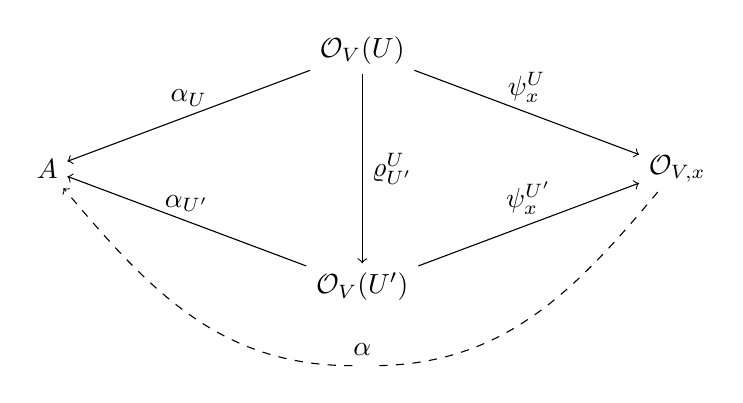
\begin{tikzpicture}
		%definiere die Punkte
		\node (OVU) at (0,1.5) {$\calO_V(U)$};
		\node (OVU') at (0,-1.5) {$\calO_V(U')$};
		\node (A) at (-4,0) {$A$};
		\node (OVX) at (4,0) {$\calO_{V,x}$};
		\node (nix) at (0,-2.5) {};
		%zeichne die Pfeile
		\draw[->](OVU) --node[right]{$\varrho_{U'}^U$} (OVU');
		\draw[->](OVU) --node[above]{$\alpha_U$} (A);
		\draw[->](OVU) --node[above]{$\psi_x^U$} (OVX);
		\draw[->](OVU') --node[above]{$\alpha_{U'}$} (A);
		\draw[->](OVU') --node[above]{$\psi_x^{U'}$} (OVX);
		\draw[dashed, ->](OVX) to[out=230, in=0] (nix) node[above]{$\alpha$} to[out=180, in=310] (A);
	\end{tikzpicture}\end{center}
\item\label{bem15.3c}
	$\psi_x^U$ ist injektiv, falls $U\subset \bigcup\limits_{\substack{V_i\text{ irred. Komp.}\\\text{v. } V \text{ mit }x\in V_i}} V_i$
\end{enumerate}\end{Bem}

\begin{Prop}\label{prop15.4}
Seien $V,x$ wie in Definition \ref{def15.1}, $V_0\subseteq V$ offen, affin mit $x\in V_0$. Dann ist $\calO_{V,x}\cong k[V_0]_{m_x^{v_0}}$, wobei $m_x^{v_0}={f \in k[V_0] | f(x)=0}$, insbesondere ist $\calO_{V,x}$ von $V_0$ unabh\"angig
\end{Prop}

\begin{Bew}
Sei $\alpha:k[V_0]_{m_x^{V_0}}\to \calO_{V,x}, \frac{f}{g}\mapsto(D(g),y\mapsto\frac{f(y)}{g(y)})_\sim$

$\alpha$ ist wohldefinierter $k$-Algebra-Homomophismus.
\begin{description}[\setlabelstyle{\itshape}]
\item[$\alpha$ ist injektiv:]
	Sei $\alpha(\frac{f}{g})=0$
	
	Dann gibt es $U\subset G(g)$ offen mit $f(y)=0$ f\"ur alle $y\in U$.
	
	$\Rightarrow W=V_0-U$ ist abgeschlossen in $V_0, x\notin W$
	
	$\Rightarrow $ Dann gibt es $h\in I(W)$ mit $h(x)\ne0$ (weil $V(I(W))=W$ ist)
	
	$\Rightarrow h\notin m_y^{V_0}$ mit $h(y)\cdot f(y)=0$ f\"ur alle $y\in V_0$
	
	$\Rightarrow f=0$ in $k[V_0]_{m_x^{V_0}}$
	
	$\Rightarrow \frac{f}{g}=0$ in $k[V_0]_{m_x^{V_0}}$
\item[$\alpha$ ist surjektiv:]
	Sei $(U,f)_\sim\in\calO_{V,x}$
	
	\OE $U\subseteq V_0, U=D(h)$ f\"ur ein $h\in k[V_0]$
	
	$\Rightarrow f\in\calO_V(U)=\calO_{V_0}(U)=k[V_0]_h$
	
	$\Rightarrow (U,f)_\sim=\alpha(\frac{g}{h^r})$
\end{description}\end{Bew}

\begin{Prop}\label{prop15.5}
Seien $V,W$ quasiprojektive Variet\"aten, $x\in V, y\in W$. Ist $\calO_{V,x}\cong\calO_{W,y}$ (als $k$-Algebren), so gibt es offene Umgebungen $U\subseteq V$ von $x$ und $U'\subseteq W$ von $y$ mit $U\cong U'$ (als quasiprojektive Variet\"aten).
\end{Prop}

\begin{Bew}
Seien $U_x\subseteq V$, beziehungsweise $U_y\subseteq W$ offene affine Umgebungen von $x$ beziehungsweise $y$ wie in \ref{bem15.3} \ref{bem15.3c}), also $\psi_x^{U_x}$ und $\psi_y^{U_y}$ injektiv. Seien $f_1,\ldots ,f_r$ Erzeuger von $\calO_V(U_x)=k[U_x]$ als $k$-Algebra. Sei weiter $\varphi:\calO_{V,x}\to\calO_{W,y}\cong k[U_y]_{m_x^{U_y}}$ ein Isomorphismus.

F\"ur die Keime gilt also: $(f_i)_x=\frac{g_i}{h_i}$ mit $h_i, g_i \in k[U_y], h_i(y)\ne 0, i=1,\ldots ,r$

Sei $U_y' \subseteq U_y$ offen, affin mit $\frac{g_i}{h_i}\in\calO_W(U_y'), i=1,\ldots ,r$ (also z. B. $U_y'=U_y\cap D(h_1)\cap\ldots \cap D(h_r)$)

$\Rightarrow \varphi\circ\psi_x^{U_x}$ induziert injektiven $k$-Algebra-Homomophismus
	\[k[U_x]\to k[U_y']\]
Dieser entspricht dominantem Morphismus $f:U_y'\to U_x$. Genauso erhalten wir dominanten Morphismus $g:U_x'\to U_y$.

$f$ und $g$ sind zueinander inverse rationale Abbildung $U_x \overset{\dashleftarrow}{\to} U_y$ %Da muss es eine bessere Moeglichkeit geben? extpfeil koennte das
\end{Bew}

\begin{Bem}
Sei $\varphi: V\to W$ Morphismus von quasiprojektiven Variet\"aten, $x\in V$. Dann induziert $\varphi$ einen $k$-Algebra-Homomophismus
	\[\varphi_x^{\#}:\calO_{W,\varphi(x)}\to\calO_{V,x} \text{ mit } \varphi_x^{\#}(m_{\varphi(x)})\subseteq m_x\]
\end{Bem}

\begin{Bew}
\OE $V,W$ affin (wegen Proposition \ref{prop15.4}).

$\varphi$ induziert $\varphi^\#:k[W]\to k[V]$ (durch $f\mapsto f\circ\varphi$).

Dabei ist $f\in m_{\phi(x)}^W, f(\varphi(x))=0 \Leftrightarrow (f\circ\varphi)(x)=0 \Leftrightarrow \varphi^\#(f)\in m_x^V$

$\Rightarrow \varphi^\#$ induziert
	\[ \varphi_x^\#: \underbrace{k[W]_{m_{\varphi(x)}^W}}_{=\calO_{W,\varphi(x)}} \to \underbrace{k[V]_{m_x^V}}_{=\calO_{V,x}}\]
mit $\varphi_x^\#(m_{\varphi(x)}) = \varphi_x^\#(m_{\varphi(x)}^W \cdot k[W]_{m_{\varphi(x)}^W}) \subseteq m_x^V \cdot k[V]_{m_x^V} = m_x$
\end{Bew}

\newpage

%-------------------------- Abschnitt 16 --------------------------

\section{Tangentialraum}

\begin{Bsp}\begin{enumerate}[a)]
\item
	$V_1=\underbrace{V(Y^2-X^3+X)}_{Y^2=X(X-1)(X+1)}, x(0,0)$
	
	\begin{minipage}{0.7\linewidth}Tangente an $V_1$ in $x$ \quot{ist} die $y$-Achse.\end{minipage}
	\begin{minipage}{0.3\linewidth}\begin{flushright}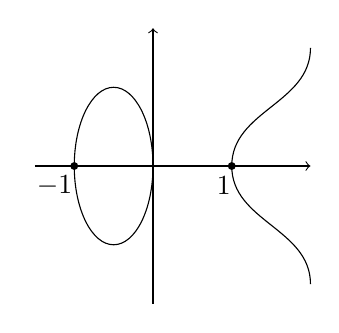
\begin{tikzpicture}
		\draw[->] (-1.5,0) -- (2,0); \draw[->] (0,-1.75) -- (0,1.75);
		
		\draw (-0.5,0) circle[x radius=0.5, y radius=1]; \draw (2,1.5) to[out=270,in=90] (1,0) to[out=270,in=90] (2,-1.5);
		
		\node at (-1.25,-0.25) {$-1$}; \node at (0.9,-0.25) {$1$};
		\fill (-1,0) circle[radius=0.05]; \fill (1,0) circle[radius=0.05];
	\end{tikzpicture}\end{flushright}\end{minipage}
\item
	$V_2=\underbrace{V(Y^2-X^3-X^2)}_{Y^2=X^2(X+1)}, x=(0,0)$
	
	\begin{minipage}{0.7\linewidth}Es gibt zwei Tangenten in $x$ an $V_2$. Jede Gerade durch $x$ ist Grenzwert von Sekanten.\end{minipage}
	\begin{minipage}{0.3\linewidth}\begin{flushright}\begin{tikzpicture}
		\draw[->] (-1.5,0) -- (2,0); \draw[->] (0,-1.75) -- (0,1.75);
		
		\draw (1,1) to[out=225,in=45] (0,0) to[out=225,in=270] (-1,0) to[out=90,in=135] (0,0) to[out=315,in=135] (1,-1);
		
		\node at (-1.25,-0.25) {$-1$}; \fill (-1,0) circle[radius=0.05];
	\end{tikzpicture}\end{flushright}\end{minipage}
\item
	$V_3=V(Y^2-X^3), x=(0,0)$
	
	\begin{minipage}{0.7\linewidth}Die $x$-Achse ist (Doppel-)Tangente. Jede Gerade durch $x$ ist Limes von Sekanten.\end{minipage}
	\begin{minipage}{0.3\linewidth}\begin{flushright}\begin{tikzpicture}
		\draw[->] (-1.5,0) -- (2,0); \draw[->] (0,-1.75) -- (0,1.75);
		
		\draw (1.5,1.5) to[out=270,in=0] (0,0) to[out=00,in=90] (1.5,-1.5);
	\end{tikzpicture}\end{flushright}\end{minipage}
\end{enumerate}\end{Bsp}

\begin{Erinn}[Taylorentwicklung]
Sei $f\in k[X_1,\ldots ,X_n], x=(x_1,\ldots ,x_n)\in k^n$.\begin{enumerate}[a)]
\item
	$f=\Sum_{(\nu_1,\ldots ,\nu_n)\in \N^n} \frac{1}{(\nu_1+\ldots +\nu_n)!}\frac{\partial\nu_1}{\partial X_1}\cdot\ldots \cdot \frac{\partial\nu_n}{\partial X_n} f(x)(X_1-x_1)^{\nu_1}\cdot\ldots \cdot(X_n-x_n)^{\nu_n}$
\item
	$f=f(x)+ \underbrace{\Sum_{i=1}^n\frac{\partial f}{\partial(X_i)}(x)(X-x_i)}_{\in m_x} + \underbrace{\text{ h\"ohere Terme (Grad} \ge2)}_{\in m_x^2}$
\end{enumerate}\end{Erinn}

\begin{DefBem}\label{16.3}
Sei $f \in k[X_1,\ldots ,X_n], x=(x_1,\ldots ,x_n)$\begin{enumerate}[a)]
\item
	$f_x^{(1)}:=\Sum_{i=1}^n\frac{\partial f}{\partial X_i}(x)X_i =:D_x(f)$
\item
	Sei $V\subseteq \A^n(k)$ affine Variet\"at mit $x\in V, I:=I(V)\subseteq k[X_1,\ldots ,X_n]$
	
	$I_x:=\langle\{f_x^{(1)}:f\in I\}\rangle$
	
	$T_{V,x}:=V(I_x)$ hei\ss t Tangentialraum an $V$ in $x$.
\item
	Wird $I$ von $f_1,\ldots ,f_r$ erzeugt, so wird $I_x$ von $(f_1^{(1)})_x,\ldots ,(f_r^{(1)})_x$ erzeugt.
\item\label{16.3d}
	$T_{V,x}$ ist linearer Unterraum von $k^n$, genauer
		\[ T_{V,x}=\Kern\left( \frac{\partial f_i}{\partial X_j}(x) \right)_{\begin{subarray}{l}i=1,\ldots ,r\\j=1,\ldots ,m\end{subarray}}\]
	(Jacobi-Matrix der Abbildung $f:k^n\to k^r, x\mapsto(f_1(x),\ldots ,f_r(x)$)
\end{enumerate}\end{DefBem}

\begin{Bew}\begin{enumerate}[a)]\item[c)]
Sei $g\in I$ beliebig, schreibe $g=\Sum_{i=1}^r g_if_i, g_i\in k[X_1,\ldots ,X_n]$

$D_x(f+g)=D_x(f)+D_x(g)$

$D_x(f\cdot g)=f(x)D_x(g)+g(x)D_x(f)$

$\Rightarrow D_x(g)=\Sum_{i=1}^rD_x(g_if_i)=\Sum_{i=1}^r[g_i(x)\underset{=0, \text{ weil }x\in V \text{ und } f_i\in I(V)}{D_x(f_i)+\underbrace{f_i(x)}D_x(g_i)}] = \Sum_{i=1}^rg_i(x)(f_i^{(1)})_x$
\end{enumerate}\end{Bew}

\begin{nnBsp}[Noch einmal Bsp. 16.1]\begin{enumerate}[a)]
\item
	$V_1=V(f)$ mit $f=Y^2-X^3+X, x=(0,0)$
	
	$\Rightarrow f_x^{(1)}=1\cdot X+0\cdot Y=X$
	
	$\Rightarrow T_{V,x}=V(X)= y$-Achse
\item
	$V_2=V(f)$ mit $f=Y^2-X^3-X^2, x=(0,0)$
	
	$\Rightarrow f_x^{(1)}=0$, also $T_{V,x}=k^2$
\item
	Genauso
\end{enumerate}\end{nnBsp}

\begin{Prop}
Sei $\varphi:V\to W$ ein Morphismus affiner Variet\"aten, $V\subseteq \A^n(k), W\subseteq \A^m(k)$. Dann induziert $\varphi$ f\"ur jedes $x\in V$ eine $k$-lineare Abbildung
	\[ d_{x\varphi}: T_{V,x}\to T_{W,\varphi(x)} \]
\end{Prop}

\begin{Bew}
Sei $\varphi:V\to W$ gegeben durch $x\mapsto(\varphi_1(x),\ldots ,\varphi_m(x)), \varphi_i\in k[X_1,\ldots ,X_n]$. Der zugeh\"orige $k$-Algebra-Homomophismus
	\[k[W]=\FakRaum{k[Y_1,\ldots ,Y_m]}{I(W)}\to \FakRaum{k[X_1,\ldots ,X_n]}{I(V)}=k[V]\]
wird induziert von $\varphi^\#:k[Y_1,\ldots ,Y_m]\to k[X_1,\ldots ,X_n], f\mapsto f\circ \varphi_i$.

\emph{Genauer:} $\varphi^\#(Y_j)=\varphi_j$

Dabei ist $\varphi^\#(I(W))\subseteq I(V)$, da $\varphi(V)\subseteq W$. Definiere $\alpha: k[Y_1,\ldots ,Y_m]\to k[X_1,\ldots ,X_n]$ durch $Y_j\mapsto D_x(\varphi^\#(Y_j))=D_x(\varphi_j)=(\varphi_j^{(1)})_x$.

\emph{Behauptung:} $\alpha(I_{\varphi(x)})\subseteq I_x$

Dann induziert $\alpha$ einen $k$-Algebra-Homomophismus
	\[ \underset{=k[T_{W,\varphi(x)}]}{\FakRaum{k[Y_1,\ldots ,Y_m]}{I_{\varphi(x)}}} \to \underset{=k[T_{V,x}]}{\FakRaum{k[X_1,\ldots ,X_n]}{I_x}} \]
Und damit Morphismus $T_{V,x}\to T_{W,\varphi(x)}$

\begin{description}[\setlabelstyle{\itshape}]
\item[Beweis der Behauptung:]
	Sei $g\in I_{\varphi(x)}$

	\OE $g=h^{(1)}$ f\"ur ein $h\in I(W)$

	$\alpha(g) =$ (Weihnachtsrechnung) $= D_x(g\circ \varphi)\in I_x$
\end{description}
\end{Bew}

% 09.01.2011
\begin{nnErinn}
$V$ affine Variet\"at \"uber einem K\"orper $k$, $x\in V$.

$T_{V,x} =V(I_x), I_x$ erzeugt von den $f_x^{(1)}=\Sum_{i=1}^n\frac{\partial f}{\partial X_i}(x)X_i, f\in I(V)$. Die Zuordnung $(V,x)\mapsto T_{V,x}$ ist ein kovarianter Funktor
	\[ \underline{\text{(affine Variet\"aten)}/k + \text{Punkt}} \to \underline{k\text{-Vektorr\"aume}}\]
\end{nnErinn}

\newpage

%-------------------------- Abschnitt 17 --------------------------

\section{Derivationen und Zariski-Topologie}

\begin{Def}\label{Def17.1}
Sei $R$ Ring (kommutativ mit Eins), $A$ eine $R$-Algebra, $M$ ein $A$-Modul. Eine $R$-lineare Abbildung $D:A\to M$ hei\ss t \deftermspec{$R$-Derivation}{Derivation}, wenn gilt:
	\[ D(f\cdot g)=f\cdot D(G) + g\cdot D(f) \qquad \text{f\"ur alle }f,g \in A\]
\end{Def}

\begin{Bsp}\label{Bsp17.2}\begin{enumerate}[a)]
\item\label{Bsp17.2a}
	Sei $A=M=R[X], D(f):=\frac{df}{dg}$
	
	Konkret: $D(\Sum_{i=0}^n a_iX^i)=\Sum_{i=1}^nia_iX^{i-1}$
	
	\emph{$D$ ist Derivation:} Nachrechnen!!!
\item
	$A=M=R[X_1,\ldots ,X_n], D_i=\frac{\partial}{\partial X_i}$
\item\label{Bsp17.2c}
	$A=R[X_1,\ldots ,X_n], M=R, x=(x_1,\ldots ,x_n)\in \R^n$
	
	$M$ wird zum $A$-Modul durch $\varphi_x(f)=f(x)$ (Einsetzungshomomophismus).
	
	$D(f):=\frac{\partial f}{\partial X_i}(x)$ ist $R$-Derivation, \emph{denn:}
	
	$D(fg)=(\frac{\partial}{\partial X_i}(fg))(x)=(f\frac{\partial g}{\partial X_i}+g\frac{\partial f}{\partial X_i})(x) = f(x)\frac{\partial g}{\partial X_i}(x) + g(x)\frac{\partial f}{\partial X_i}(x) = f\cdot D(g) + g\cdot D(f)$
\end{enumerate}\end{Bsp}

\begin{Bem}\label{Bem17.3}Seien $R,A,M$ wie in \ref{Def17.1}\begin{enumerate}[a)]
\item
	F\"ur jede $R$-Derivation $D:A\to M$und jedes $a\in R$ gilt $D(a)=0$.
\item
	$\Der_R(A,M)=\{D:A\to M| D \text{ ist Derivation}\}$ ist $A$-Modul.
\item\label{Bem17.3c}
	Ist $\varphi:M_1\to M_2$ ein Homomophismus von $A$-Moduln, so ist \[\begin{array}{rcl}\Der_R(A,M_1)&\to&\Der_R(A,M_2)\\D&\mapsto&\varphi\circ D\end{array}\] ein Homomophismus von $A$-Moduln.
\item
	Die Zuordnung $M\mapsto\Der_R(A,M)$ ist ein kovarianter Funktor:
		\[ \underline{A\text{-Moduln}} \to \underline{A\text{-Moduln}} \]
\end{enumerate}\end{Bem}

\begin{Bew}\begin{enumerate}[a)]
\item
	$D(1)=D(1\cdot1)=1\cdot D(1) + 1\cdot D(1) \Rightarrow D(1)=0 \overset{D\text{ ist }R\text-linear}{\Longrightarrow }D(a)=D(a\cdot 1)=a\cdot D(1)=0$
\item
	$\checkmark$
\item
	$(\varphi\circ D)(f\cdot g)=\varphi(f\cdot D(g)+g\cdot D(f))\overset{\varphi A\text{-Mod-Hom}}{=} f\cdot \varphi(D(g))+ g\cdot\varphi(D(f))$
\end{enumerate}\end{Bew}

\begin{Bem}\label{bem17.4}\begin{enumerate}[a)]
\item
	F\"ur $A=R[X]$ ist $\Der_R(A,A)=A\cdot D$ ($D=\frac{d}{dX}$ wie in \ref{Bsp17.2} \ref{Bsp17.2a}))
\item
	F\"ur $A=R[X_1,\ldots ,X_n]$ ist $\Der_R(A,A)$ der freie $A$-Modul mit Basis $\frac{\partial}{\partial X_1},\ldots ,\frac{\partial}{\partial X_n}$
\item\label{bem17.4c}
	Sei $A=R[X_1,\ldots ,X_n], x=(x_1,\ldots ,x_n), M=R$ wie in \ref{Bsp17.2} \ref{Bsp17.2c}).
	
	$\Rightarrow \Der_R(A,R)$ ist der von den $\frac{\partial}{\partial X_i}(x)$ erzeugte freie $R$-Modul.
\end{enumerate}\end{Bem}

\begin{Bew}\begin{enumerate}[a)]
\item
	Sei $\delta: A\to A$ $R$-Derivation, $f:=\delta(X)$. $\Rightarrow \delta(X^2) = X\cdot\delta(X)+X\cdot\delta(X)=2f\cdot X$
	
	$\overset{\text{Induktion}}{\Longrightarrow} \delta(X^n)=n\cdot f\cdot X^{n-1} \Rightarrow \delta(\Sum_{i=0}^na_iX^i) = f\cdot \Sum_{i=1}^nia_iX^{n-1} \Rightarrow \delta=f\cdot D$
\item[c)]
	folgt aus b) und \ref{Bem17.3} \ref{Bem17.3c}).
\end{enumerate}\end{Bew}

\begin{Prop}\label{prop17.5}
Sei $V\subseteq\A^n(k)$ affine Variet\"at, $x=(x_1,\ldots ,x_n)\in V, \calO_{V,x}=\{\frac{f}{g}: f,g\in k[V], g(x)\ne 0\}$. Dann ist $\Der_R(\calO_{V,x},k)\cong(m_x/m_x^2)^v$ (Isomorphismus von $k$-Vektror\"aumen).

$\Der_R(\calO_{V,x},k)$ und $m_x/m_x^2$ sind $\calO_{V,x}$-Moduln, in beiden Moduln ist die Multiplikation mit einem Element aus $m_x$ die Nullabbildung.

$\Rightarrow $ Beide Moduln sind Moduln \"uber $\calO_{V,x}/m_x=k$
\end{Prop}

\begin{Bew}
Sei $\delta \in \Der_R(\calO_{V,x},k)$. $\delta|_{m_x}$ ist $k$-linear.

\emph{Behauptung:} $m_x^2\subseteq\Kern(\delta)$

\emph{denn:} Sei $f=g\cdot h\in m_x^2, g, h\in m_x \Rightarrow \delta(f) = \underbrace{g(x)}_{=0}\cdot\delta(h)+\underbrace{h(x)}_{=0}\cdot \delta(g)=0$

$\Rightarrow \delta$ induziert $k$-lineare Abbildung $m_x/m_x^2 \to k$.

Sei umgekehrt $l\in (m_x/m_x^2)^v$. Definiere $\delta: \calO_{V,x}\to k$ durch $\delta(f):=l(\overline{\underbrace{f-f(x)}_{\in m_x}})$ ($k$-linear: $\checkmark$).

Seien $f,g\in \calO_{V,x}$. Dann ist $(f-f(x))(g-g(x))\in m_x^2$.

$\Rightarrow 0=l((f-f(x))(g-g(x))) = l(fg-f(x)g(x)-fg(x)-gf(x)+2f(x)g(x))$

$\Rightarrow \delta(fg)= l(fg(x)+gf(x)-2f(x)g(x)) = f(x)l(g-g(x))+g(x)l(f-f(x)) = f\delta(g)+g\delta(f)$
\end{Bew}

\begin{SatzDef}\label{satz8}
Sei $V$ affine Variet\"at, $x\in V$. Dann gibt es einen nat\"urlichen Isomorphismus
	\[ T_{V,x} \cong (\FakRaum{m_x}{m_x^2})^v\]
$(m_x/m_x^2)^v$ hei\ss t \defterm{Zariski-Tangentialraum} an $V$ in $x$.
\end{SatzDef}

\begin{Bew}\begin{enumerate}[i)]
\item
	Definiere Abbildung\\ 
	\begin{center}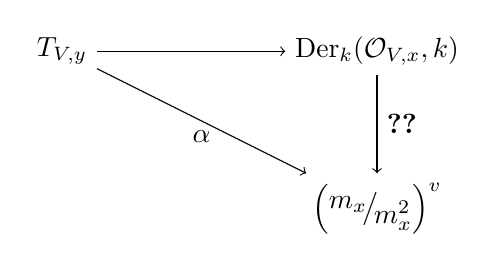
\begin{tikzpicture}
		%Punkte definieren
		\node (T) at (0,0) {$T_{V,y}$};
		\node (Der) at (4,0) {$\Der_k(\calO_{V,x},k)$};
		\node (m) at (4,-2) {$\left(\FakRaum{m_x}{m_x^2}\right)^v$};
		%Pfeile zeichnen
		\draw[->](T) -- (Der);
		\draw[->](T) --node[below]{$\alpha$} (m);
		\draw[->](Der) --node[right]{\ref{prop17.5}} (m);
	\end{tikzpicture}\end{center}
	Jedes $y=(y_1,\ldots ,y_n)\in k^n$ induziert Derivation $D_y:k[X_1,\ldots ,X_n]\to k$ durch $f\mapsto\sum	\limits_{i=1}^n\frac{\partial f}{\partial X_i}(x)y_i$ (\ref{bem17.4} \ref{bem17.4c})). Ist $y \in T_{V,x}$ und $f\in I(V)$, so ist $D_y(f)=0$ nach Definition, denn $D_y(f)=f_x^1(y)$.
	
	$\Rightarrow D_y$ induziert Derivation $D_y:k[V]\to k$.
	
	F\"ur $\frac{f}{g}\in \calO_{V,x}$ sei $D_y(\frac{f}{g})=\frac{g(x)D_y(f)-f(x)D_y(g)}{g(x)^2}$ (denn $D_y(\frac{f}{g}\cdot g)=D_y(f) \Rightarrow D_y$ induziert $D_y\in \Der_R(\calO_{V,x},k)$)
	
%11.01.2012
	\emph{Noch zu zeigen:} $\frac{f}{g}=0$ in $\calO_{V,x}\Rightarrow \frac{-f(x)D_y(g)+g(x)D_y(f)}{g(x)^2}=0$
	
	\emph{denn:} $\frac{f}{g}=0$ in $\calO_{V,x} \Rightarrow \exists h\in \calO_{V,x}\setminus m_x$ mit $h\cdot f=0$ in $k[V]$ $\Rightarrow 0=D_y(hf)=\overbrace{h(x)}^{\ne0}D_y(f)+\underbrace{f(x)}_{=0}D_y(h)$ $\Rightarrow D_y(f)=0$ $\Rightarrow D_y(\frac{f}{g})=0$
\item
	$ \beta:\begin{array}{rcl}(m_x/m_x^2) &\to& T_{V,x}\\
	l &\mapsto& \left(l(\overline{X_1-x_1}),\ldots ,l(\overline{X_n-x_n})\right)\end{array}$
	
	\emph{Zu zeigen:} $\left(l(\overline{X_1-x_1}),\ldots ,l(\overline{X_n-x_n})\right) \in T_{V,x}$
	
	Sei dazu $f\in I(V)$. \emph{Zu zeigen:} $f_x^{(1)}\left(l(\overline{X_1-x_1}),\ldots ,l(\overline{X_n-x_n})\right)=0$
	
	Es ist $f_x^{(1)}\left(l(\overline{X_1-x_1}),\ldots ,l(\overline{X_n-x_n})\right)= \Sum_{i=1}^n \frac{\partial f}{\partial X_i}(x)l(\overline{X_i-x_i})$ $= l\left(\Sum_{i=1}^n \frac{\partial f}{\partial X_i}(x)(X_i-x_i)\right)$ $\overset{(*)}{=}$ $l\left( f_x^{(1)}-f_x^{(1)}(x) \right) = 0$, wegen
	
	\emph{Behauptung:} $f_x^{(1)}-f_x^{(1)}(x)\in m_x^2$
	
	\emph{denn:} Taylor-Entwicklung $\underbrace{f}_{0\text{ in }k[V]}= \underbrace{f(x)}_{=0\text{, weil }f\in I(V)}+f_x^{(1)}-f_x^{(1)}(x)+ $Terme in $m_x^2$
\item
	$\beta\circ\alpha=\id_{T_{V,x}}$
	
	$\beta(\alpha(y))= \beta(f\mapsto\Sum_{i=1}^n\frac{\partial f}{\partial X_i}(x)y_i) = \left(\Sum_{i=1}^n\frac{\partial(X_1-x_1)}{\partial X_i}(x)y_i,\ldots ,\Sum_{i=1}^n\frac{\partial(X_n-x_n)}{\partial X_i}(x)y_i\right) = (y_1,\ldots ,y_n)$
\item
	$\alpha\circ\beta=\id_{(m_x/m_x^2)^v}$
	
	$\alpha\bigl(\beta(l)\bigr)(f)= \alpha\bigl(l(X_1-x_1),\ldots ,l(X_n-x_n)\bigr)(f) = \Sum_{i=1}^n\frac{\partial f}{\partial X_i}(x)l(X_i-x_i) \overset{(*)}{=} l\left(f_x^{(1)}-f_x^{(1)}(x)\right) = l(\overline f)$
\end{enumerate}\end{Bew}

\newpage

%-------------------------- Abschnitt 18 --------------------------

\section{Dimension einer Variet\"at}

\begin{Def}
Sei $X$ topologischer Raum. Dann hei\ss t
	\[\dim(X):=\sup\{n\in\N:\exists\text{ Kette }\emptyset\ne V_0\subsetneq,\ldots ,\subsetneq V_n\text{ von irred. abgeschl. Teilm. v. }X\}\]
\defterm{Krull Dimension} von $X$.
\end{Def}

\begin{nnBsp}\begin{enumerate}[1)]
\item
	$\dim(\R^n)=0$ f\"ur jedes $n\ge0$ (mit euklidischer Topologie)
\item
	$\dim(\A^1(k))=1$, falls $k$ unendlich ist
\item
	$\dim(\A^n(k))\ge n$, falls $k$ unendlich ist f\"ur $n\ge2$
\end{enumerate}\end{nnBsp}

\begin{Bem}\label{bem18.2}
Sei $X$ ein topologischer Raum\begin{enumerate}[a)]
\item
	Ist $Y\subseteq X$ (mit Spurtopologie), so ist $\dim(Y)\le\dim(X)$.
\item\label{bem18.2b}
	Ist $X=\bigcup\limits_{i=1}^nX_i$, $X_i$ abgeschlossen, so ist $\dim(X)=\max_{i=1}^n(\dim(X_i))$.
\end{enumerate}\end{Bem}

\begin{Bew}\begin{enumerate}[a)]
\item
	Sei $\emptyset\ne V_0\subsetneq,\ldots ,\subsetneq V_d$ Kette von abgeschlossenen Teilmengen von $Y$. Sei $\overline{V_i}$ der Abschluss von $V_i$ in $X$.
	
	$V_i$ ist irreduzibel nach \"Ubung 2, Aufgabe 5.
	
	$\overline{V_i}\cap Y=V_i$ weil $V_i$ abgeschlossen in $Y$ ist. $\Rightarrow \overline{V_i}\subsetneq\overline{V}_{i+1}$
	
	$\Rightarrow \emptyset\ne V_0\subseteq\ldots \subseteq V_d$ ist Kette der L\"ange $d$ in $X$.
\item\begin{twosidedproofeq}
\proofge
	gilt nach a)
\proofle
	Sei $\emptyset\ne V_0\subsetneq,\ldots ,\subsetneq V_d$ Kette in $X$. Dann ist $V_d=V_d\cap(\bigcup\limits_{i=1}^nX_i)=\bigcup\limits_{i=1}^n(\underbrace{V_d\cap X_i}_{\text{abg. in }V_d})$
	
	$V_d$ irreduzibel $\Rightarrow \exists i$ mit $V_d\subseteq X_i \Rightarrow d\le \dim(X_i)$
\end{twosidedproofeq}\end{enumerate}\end{Bew}

\begin{Def}
Sei $R$ ein Ring (das hei\ss t kommutativ mit Eins)\begin{enumerate}[a)]
\item
	Sei $\mathfrak p \in R$ Primideal. Dann hei\ss t
		\[\Ht(\mathfrak p):=\sup\{n\in\N:\exists \p_0\subseteq\ldots \subseteq\p_n=\p \text{ Kette von Primelementen in }R\}\]
	\defterm{H\"ohe} von $\p$.
\item
	$\dim(R):=\sup\{\Ht(\p):\p\subset R \text{ Primideal}\}$ hei\ss t \defterm{Krull Dimension}.
\end{enumerate}\end{Def}

\begin{nnBsp}\begin{enumerate}[1)]
\item
	$\dim k=0$ f\"ur jeden K\"orper $k$
\item
	$\dim\Z=1$
\item
	$\dim k[X]=1$ f\"ur jeden K\"orper $k$
\item
	$\dim \Z[X]=2$ (\"Ubung?)
	
	$(0)\subset(2)\subset(2,X)$
\item
	$\dim k[X,Y]=2$??
\end{enumerate}\end{nnBsp}

\begin{Prop}
Ist $k$ algebraisch abgeschlossen, so gilt f\"ur jede affine Variet\"aten $V\subseteq\A^n(k)$: $\dim(V)=\dim k[V]$
\end{Prop}

\begin{Bew}
Wegen V(I) irred. für I prim und I(V(I))$\overset{\textrm{HNS}}{=}$I sowie I(V) prim für V irred. und V(I(V))$=$V folgt, dass die eine Kette eine gültige andere Kette ist.
\end{Bew}

\begin{Satz}
Sei $k$ ein K\"orper, $A$ endlich erzeugte nullteilerfreie $k$-Algebra.\begin{enumerate}[a)]
\item
	$\dim k[X_1,\ldots ,X_n]=n$
\item
	Ist $\varphi:k[X_1,\ldots ,X_n]\to A$ surjektiver Homomophismus von $k$-Algebren, so ist \[\dim A +\Ht(\Kern(\varphi))=n\]
\item
	Jede maximale (nicht verl\"angerbare) Kette von Primidealen in $A$ hat die L\"ange $A$.
\end{enumerate}\end{Satz}

\begin{nnErinn}
$S|R$ \deftermspec{ganze Ringerweiterung}{Ring!-erweiterung!ganze} $\Leftrightarrow$ jedes $a\in S$ ist Nullstelle eines \emph{normierten} Polynoms mit Koeffizienten aus $R$.
\end{nnErinn}

\begin{UnterSatz}\label{satz9.1}
Sei $S|R$ ganze Ringerweiterung.\begin{enumerate}[a)]
\item\label{satz9.1a}
	(\quot{Going Up}) F\"ur jede Primidealkette $\mathfrak p_0\subsetneq\ldots \subsetneq \mathfrak p_n$ in $R$ gibt es eine Primidealkette $\mathfrak P_0\subsetneq\ldots \subsetneq \mathfrak P_n$ in $S$ mit $\mathfrak P_i\cap R=\mathfrak p_i$ f\"ur $i=0,\ldots ,n$.
\item
	$\dim S = \dim R$
\end{enumerate}\end{UnterSatz}

\begin{UnterSatz}[\quot{Noether-Normalisierung}]
Sei $A$ endlich erzeugte $k$-Algebra. Dann ist $A$ ganze Ringerweiterung eines Polynomrings \"uber $k$.

\emph{Genauer:} F\"ur jedes echte Ideal $I\subset A$ gibt es algebraisch unabh\"angige Elemente $x_1,\ldots ,x_d\in A$, sodass $A$ ganz ist \"uber $k[x_1,\ldots ,x_d]$ und $I\cap k[x_1,\ldots ,x_d]=(x_{\delta+1},\ldots ,x_d)$ f\"ur ein $0\le\delta\le d$.
\end{UnterSatz}

\begin{nnBsp}
$A=k[V]$ f\"ur affine Variet\"at $V$. $k[x_1,\ldots ,x_d] \hookrightarrow A$ Noether-Normalisierung induziert $\varphi:V\to\A^d(k)$. $\varphi$ ist surjektiv nach Satz \ref{satz9.1} \ref{satz9.1a}).

\textcolor{red}{Der Bew. wird noch nachgef\"ugt}
\end{nnBsp}

\begin{UnterSatz}
(\quot{Going Down}) Sei $A$ endlich erzeugte nullteilerfreie $k$-Algebra, $k[x_1,\ldots ,x_d]\hookrightarrow A$ Noether-Normalisierung, $\mathfrak P_1\subset A$ Primideal, $\mathfrak p_0$ Primideal mit $\mathfrak p_0 \subset \mathfrak p_1 := \mathfrak P_1\cap B$. Dann gibt es Primideale $\mathfrak P_0\subset \mathfrak P_1$ mit $\mathfrak P_0\cap B=\mathfrak p_0$.
\begin{center}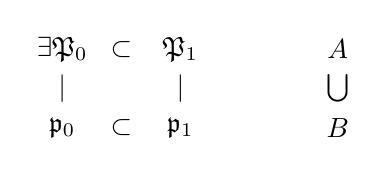
\begin{tikzpicture}
	%Punkte zeichnen
	\node (P0) at (-1.75,0) {$\exists\mathfrak P_0$};
	\node (P1) at (-0.25,0) {$\mathfrak P_1$};
	\node (A) at (1.75,0) {$A$};
	\node (P0) at (-1.75,-1) {$\mathfrak p_0$};
	\node (P0) at (-0.25,-1) {$\mathfrak p_1$};
	\node (P0) at (1.75,-1) {$B$};
	%Zeichen
	\node at (-1,0) {$\subset$};
	\node at (-1,-1) {$\subset$};
	\node at (1.75,-0.5) {$\bigcup$};
	\node at (-0.25,-0.5) {$|$};
	\node at (-1.75,-0.5) {$|$};
\end{tikzpicture}\end{center}
\end{UnterSatz}

\begin{Folg}\label{folg18.5}\begin{enumerate}[a)]
\item
	ist $k$ unendlich, so ist $\dim\A^n(k)=n$.
\item\label{folg18.5b}
	Ist $k$ algebraisch abgeschlossen, so gilt f\"ur jede irreduzible affine Variet\"at $V\subseteq\A^n(k)$:
		\[\dim V + \Ht(I(V))=n\]
\item\label{folg18.5c}
	Ist $k$ algebraisch abgeschlossen, so gilt f\"ur jede irreduzible affine Variet\"at $V\subseteq\A^n(k)$ und $x\in V$:
		\[\dim\calO_{V,x}=\dim k[V]_{m_x}=\Ht(m_x)=\dim k[V]=\dim V\]
\end{enumerate}\end{Folg}

\begin{DefBem}\label{18.6}
Sei $V$ eine quasiprojektive Variet\"at \"uber algebraisch abgeschlossenem K\"orper $k$, $x\in V$, $V_0\subseteq V$ offene affine Umgebung von $x$.\begin{enumerate}[a)]
\item
	$\dim_x(V)=\dim(\calO_{V,x})$ hei\ss t \deftermspec{lokale Dimension}{Dimension!lokale-} von $V$ in $x$.
\item
	$\dim_x(V)=\dim(\calO_{V,x})=\dim(\calO_{V_0,x})=\Ht(m_x^{V_0})$
\item
	Ist $V$ irreduzibel, so gilt:\begin{enumerate}[a)]
	\item[i)]
		$\dim_xV=\dim_yV$ f\"ur alle $x,y\in V$
	\item[ii)]
		Ist $U\ne\emptyset$ offen, affin in $V$, so ist $\dim U=\dim V$
	\end{enumerate}
\item
	$\dim_xV=\max\{\dim Z: Z$ irreduzible Komponente von $V$ mit $x\in Z\}$
\end{enumerate}\end{DefBem}

\begin{Bew}\begin{enumerate}[a)]
\item[c)]\begin{enumerate}[a)]
	\item[i)]
		Seien $U_x$ und $U_y$ offene affine Umgebungen von $x$, beziehungsweise $y$, $U_x\cap U_y\ne\emptyset$, da $V$ irreduzibel. F\"ur $z\in U_x\cap U_y$ gilt nach \ref{folg18.5} \ref{folg18.5c}):
			\[\dim_xV=\dim(\calO_{V,x})=\dim(\calO_{U_x,x})=\dim U_x=\dim(\calO_{U_x,z})\]
			\[=\dim_z(V)=\dim(\calO_{U_y,z})=\dim(\calO_{U_y,y})=\dim_y V\]
	\item[ii)]
		folgt aus i)\end{enumerate}
\item[d)]
	\OE $V$ affin.
	
	$\dim\calO_{V,x}=\Ht(m_x^V)=\max\{d:\exists$ Kette $\mathfrak p_0 \subsetneq\ldots \subsetneq\mathfrak p_d=m_x^V$ von Primidealen$\}$
	
	Sei $\mathfrak p_0 \subsetneq\ldots \subsetneq\mathfrak p_d=m_x^V$maximale Kette, dann ist $\mathfrak p_0$ minimales Primideal. Die minimalen Primideale entsprechen bijektiv den irreduziblen Komponenten, die $x$ enthalten (auch von $\calO_{V,x}$ ).
\end{enumerate}\end{Bew}

\begin{Folg}
Ist $k$ unendlich, so ist $\IP^n(k)=n$.
\end{Folg}

\begin{Def}\begin{enumerate}[a)]
\item
	Eine quasiprojektive Variet\"at der Dimension 1 hei\ss t (algebraische) \defterm{Kurve}.
\item
	Eine quasiprojektive Variet\"at der Dimension 2 hei\ss t (algebraische) \defterm{Fl\"ache}.
\end{enumerate}\end{Def}

\begin{Prop}
Sei $k$ algebraisch abgeschlossen, $V\subseteq\A^n(k)$ Hyperfl\"ache, also $V=V(f)$ f\"ur ein $f\in k[X_1,\ldots ,X_n]$ ($n\ge1, \deg(f)\ge1$). Dann ist $\dim V=n-1$.
\end{Prop}

\begin{Bew}
\OE $f$ irreduzibel (Bemerkung \ref{bem18.2} \ref{bem18.2b})) $\overset{\ref{folg18.5} \ref{folg18.5b})}{\Rightarrow } \dim V=n-\Ht((f))$

Sei $\mathfrak p\subset k[X_1,\ldots ,X_n]$ Primideal mit $(0)\subsetneq \mathfrak p\subseteq(f)$. W\"ahle $0\ne h\in \mathfrak p$ von minimalem Grad.

$h\in \mathfrak p\subseteq(f)\Rightarrow h=f\cdot g$ f\"ur ein $g\in k[X_1,\ldots ,X_n]$

$\mathfrak p$ Primideal $\Rightarrow \left\{\begin{array}{l}
	f\in \mathfrak p \text{ und damit } (f)=\mathfrak p\\
	\text{oder } g\in \mathfrak p \text{, da } \deg(f)\ge1\text{, ist }\deg(g)<\deg(h) \lightning \text{ zur Wahl von }h\end{array}\right.$\\
$\Rightarrow \Ht(f)=1$
\end{Bew}

\begin{nnBsp}
$V=V(XZ,YZ)\subset\A^3(k)$

$V=\underbrace{V(Z)}_{X\text{-},Y\text{-}\text{Ebene}} \cup \underbrace{V(X,Y)}_{Z\text{-}\text{Achse}}, \dim V=2$
\end{nnBsp}

%18. 01. 2012
\begin{Prop}
Sei $V\subseteq\A^n(k)$ affine Variet\"at, $I(V)=(f_1,\ldots ,f_d)$. Dann ist $\dim V\ge n-d$
\end{Prop}

\begin{Prop}[Krullscher Hauptidealsatz]\label{prop18.11}
Sei $R$ noetherscher Ring, $x\in R\setminus R^{\times}$, $\mathfrak p\subset R$ minimales Primideal mit $x\in \mathfrak p$. Dann ist $\Ht(\frakp)\le1$
\end{Prop}

\begin{Bew}
siehe Eisenbud: Commutative Algebra, Thm. 10.1
\end{Bew}

\begin{Prop}[Krullscher H\"ohensatz]
Sei $R$ noetherscher Ring, $x_1,\ldots ,x_d\in R\setminus R^{\times}$ sodass $I=(x_1,\ldots ,x_d)\ne R$. Dann ist $\Ht(\frakp)\le d$ f\"ur jedes minimale Primideal mit $I\subseteq \frakp$.
\end{Prop}

\begin{Bew}
Induktion \"uber $d$:\begin{enumerate}[$d=10$]
\item[\underline{$d=1$:}]
	Das ist \ref{prop18.11} .
\item[\underline{$d\ge2$:}]
	Sei $\frakp$ Primideal mit $I\subseteq \frakp$ und $\frakp$ sei minimal mit dieser Eigenschaft. Sei $\frakp_0\subsetneq\ldots \subsetneq \frakp_l= \frakp$ eine Primidealkette.
	
	\emph{Behauptung:} Es gibt Primidealkette $\frakq_0\subsetneq\ldots \subsetneq\frakq_{l-1}=\frakp$ mit $x_d\in\frakq_0$.
	
	Dann sei $R'=R/(x_d)$ und $\frakq_i'=\frakq_i/(x_d)$.
	
	Es ist $\frakq_0'\subsetneq\ldots \subsetneq\frakq_{l-1}'=\frakp'$ Kette von Primidealen in $R'$.
	
	$\frakp'$ ist minimal mit $x_1',\ldots ,x_d'\in \frakp'$ (bzw. $I'\subseteq\frakp'$) $\overset{\text{Ind. Vor.}}{\Longrightarrow}$ $\Ht(\frakp')\le d-1$, andererseits ist $\Ht(\frakp')\ge l-1$ $\Rightarrow $ $l-1 \le d-1$ $\Rightarrow $ $\Ht(\frakp)\le d$
\end{enumerate}
\emph{Beweis der Behauptung:}\begin{enumerate}[$l=10$]
\item[\underline{$l=1$:}]
	$\frakq_0=\frakp$ tut's.
\item[\underline{$l\ge2$:}]
	Ist $x_d\in \frakp_{l-1}$, so gibt es nach Induktionsvoraussetzung Kette $\frakq_0\subsetneq\ldots \subsetneq\frakq_{l-2}=\frakp_{l-1}$ mit $x_d\in \frakq_0$. Verl\"angere durch $\frakq_{l-1}=\frakp$. Sei also $x_d\notin \frakp_{l-1}$ und $\frakq$ minimales Primideal mit $I:=\frakp_{l-2}+(x_d)\subseteq\frakq\subseteq\frakp$.
	
	In $R'=R/\frakp_{l-2}$ ist $(0) = \frakp_{l-2}\subsetneq\frakp_{l-1}'\subsetneq\frakp'$ Kette der L\"ange 2 $\Rightarrow$ $\Ht_{R'}(\frakp')\ge2$ $\overset{\text{\ref{prop18.11} A}}{\Longrightarrow}$ $\frakp'$ ist \emph{nicht} minimal in $R'$ mit $x_d'\in\frakp'$ $\Rightarrow $ $\frakp$ ist nicht minimal in $R$ mit $(x_d)+\frakp_{l-2}\subseteq\frakp$ $\Rightarrow $ $\exists$ Primideal $\frakq$ mit $I\subseteq\frakq\subsetneq\frakp$
	
	Nach Induktionsvoraussetzung gibt es Kette $\frakq_0\subsetneq\ldots \subsetneq\frakq_{l-2}=\frakq$ mit $x_d\in\frakq_0$ $\Rightarrow $ $\frakq_0\subsetneq\ldots \subsetneq\frakq_{l-2}\subsetneq\frakq_{l-1}=\frakp$ ist gew\"unschte Kette.
\end{enumerate}\end{Bew}

\newpage

%-------------------------- Abschnitt 19 --------------------------

\section{Singularit\"aten}

\begin{Def}
Sei $V$ quasiprojektive Variet\"at \"uber einem K\"orper $k$. $x\in V$ hei\ss t \defterm{regul\"ar} (oder \deftermspec{nichtsingul\"ar}{singul\"ar!nicht-}), wenn $\dim T_{V,x}=\dim_x V$, andernfalls hei\ss t x \defterm{singul\"ar}. $V$ hei\ss t nichtsingul\"ar, wenn jeder Punkt $x\in V$ regul\"ar ist.
\end{Def}

\begin{Prop}[Jacobi-Kriterium]
Sei $V\subseteq\A^n(k)$ affine Variet\"at, $(f_1,\ldots ,f_r)$ Erzeuger von $I(V)$, $x\in V$. Dann gilt:
	\[x \text{ nichtsingul\"ar} \Leftrightarrow \Rang\underbrace{\left( \frac{\partial f_i}{\partial X_i}(x) \right)_{\begin{subarray}{l}i=1,\ldots ,r\\j=1,\ldots ,n\end{subarray}}}_{=\calJ_f(x)}=n-\dim_x V\]
\end{Prop}

\begin{Bew}
Nach Bemerkung \ref{16.3} \ref{16.3d}) ist $T_{V,x}=\Kern\left( \frac{\partial f_i}{\partial X_i}(x) \right)_{\begin{subarray}{l}i=1,\ldots ,r\\j=1,\ldots ,n\end{subarray}}$
\end{Bew}

\begin{nnBsp}
Sei $V=V(f)\subset\A^n(k)$ Hyperfl\"ache. Dann ist $\calJ_f=\left( \frac{\partial f}{\partial X_1},\ldots ,\frac{\partial f}{\partial X_n} \right)$ $\Longrightarrow$ $x$ singul\"ar $\Leftrightarrow$ $\frac{\partial f}{\partial X_1}(x)=\ldots =\frac{\partial f}{\partial X_n}(x)=0$

\emph{Konkret:}\begin{enumerate}[a)]
\item
	$V(X^2+Y^2-Z^2)\subset\A^3(k)$
	
	$\calJ_f=(2X,2Y,-2Z)$ $\Rightarrow $ $(0,0,0)$ ist der einzige singul\"are Punkt.
\item
	$V(Y^2-X^3+X)$, $\calJ=(-3X^2+1,2Y)$
	
	$(x,y)$ singul\"ar $\Rightarrow$ $y=0, 3x^2=1, x^3-x=0$ $\Rightarrow $ Es gibt keinen singul\"aren Punkt auf $V$.
\item
	Ist $\overline V\subseteq\IP^2(k)$ (mit $\overline V$ aus b)) auch nichtsingul\"ar?
	
	$\overline V=V(Y^2Z-X^3+XZ^2)$
	
	$V=\overline V\cap D(Z), \overline V=V\cup(\overline V\cap V(Z)) =\underbrace{V\cup\{(0:1:0)\}}_{=:P_\infty}$
	
	$P_\infty\in D(Y) \overline V\cap D(Y)=V(\underbrace{z-x^3+xz^2}_{=:g})$
	
	$\calJ_g=(-3x^2+z^2,1+2xz)$ $\Rightarrow $ $\calJ_g(P_\infty)=(0,1)$
	
	$\Rightarrow P_\infty$ ist regul\"arer Punkt
	
	$\Rightarrow \overline V$ ist nichtsingul\"ar
\end{enumerate}\end{nnBsp}

\begin{DefBem}\label{19.3}\begin{enumerate}[a)]
\item
	Sei $R$ noetherscher lokaler Ring mit maximalem Ideal $m$ und Restklassenk\"orper $k=R/m$. $R$ hei\ss t \defterm{regul\"ar}, wenn $\dim R=\dim_k(m/m^2)$.
\item\label{19.3b}
	Sei $V$ quasiprojektive Variet\"at \"uber $k$, $x\in V$. Dann gilt:
		\[x \text{ regul\"ar} \Leftrightarrow \calO_{V,x} \text{ regul\"ar}\]
\end{enumerate}\end{DefBem}

\begin{Bew}\begin{enumerate}[a)]
\item[b)]
	$\dim_k(m_x/m_x^2)=\dim(T_{V,x})$ (Satz \ref{satz8})
	
	$\dim \calO_{V,x}=\dim_x V$ nach Defininition \ref{18.6}
\end{enumerate}\end{Bew}

\begin{Prop}\label{19.4}\begin{enumerate}[a)]
\item
	Sei $(R,m)$ lokaler neotherscher Ring. Dann gilt: $\dim_k(m/m^2)\ge\dim R$
\item
	F\"ur jede quasiprojektive Variet\"at $V$ und jedes $x\in V$ gilt: $\dim T_{V,x}\ge\dim_xV$
\end{enumerate}\end{Prop}

\begin{Bew}\begin{enumerate}[a)]
\item[b)]
	folgt aus a) (\ref{19.3} \ref{19.3b})
\item[a)]
	\emph{Behauptung:} F\"ur $x_1,\ldots ,x_n\in m$ gilt:
		\[\{x_1,\ldots ,x_n\} \text{ minimales Erzeugersystem} \Leftrightarrow \overline{x_1},\ldots ,\overline{x_n} \text{ Basis von } \FakRaum{m}{m^2}\]
	Dann hat jedes minimale Erzeugersystem von $m$ $\dim_R(m/m^2)$ Elemente.\\
	\emph{Beweis der Behauptung:}\begin{twosidedproof}
	\proofforward
		Sei $x_1,\ldots ,x_n$ minimales Erzeugersystem.
		
		\emph{Annahme:} $\overline{x_1},\ldots ,\overline{x_n}$ linear abh\"angig, also \OE $\overline{x_1}=\Sum_{i=2}^n\lambda_i\overline{x_i}$ f\"ur gewisse $\lambda_i\in k$.
		
		$\Rightarrow x_1-\Sum_{i=2}^n\tilde{\lambda_i}x_i\in m^2$ ($\tilde{\lambda_i}\in R, \overline{\tilde{\lambda_i}}=\lambda_i$ in $R/m$)
		
		$\Rightarrow x_1-\Sum_{i=2}^n\tilde{\lambda_i}x_i = \Sum_{j=1}^n\mu_jx_1x_j+y$ mit $y\in(x_2,\ldots ,x_n)^2$
		
		$\Rightarrow x_1(\underbrace{1-\Sum_{i=i}^n\mu_jx_j}_{\in 1-m \Rightarrow \notin m \Rightarrow \in R^\times \Rightarrow x_1 \in (x_2,\ldots x_n) \lightning})\in (x_2,\ldots ,x_n)$
	\proofreverse
		\emph{zu zeigen:} $x_1,\ldots ,x_n$ erzeugen $m$
		
		Sei $N=(x_1,\ldots ,x_n)$
		
		Dann gilt $m=N+m^2$
		
		Damit folgt $m=N$ aus \ref{19.5}
	\end{twosidedproof}
\end{enumerate}\end{Bew}

\begin{Prop}[Nakayama-Lemma]\label{19.5}
Sei $(R,m)$ lokaler Ring, $M$ endlicher erzeugter $R$-Modul, $N\subseteq M$ ein Untermodul mit
	\[M=mM+N \qquad (*)\]
Dann gilt $M=N$
\end{Prop}

\begin{Bew}
\OE $N=0$, denn: Aus (*) folgt $M/N=mM/N$.

Ist dann $M/N=0$, so ist $M=N$.

\emph{Annahme:} $M\ne0$.

Denn sei $x_1,\ldots ,x_n$ minimales Erzeugersystem von $M$. Nach Voraussetzung gibt es $a_1,\ldots ,a_n\in m$ mit $x_1=\Sum_{i=1}^na_ix_i$

$\Rightarrow x_1(1-a_1)=\Sum_{i=2}^na_ix_i \Rightarrow x_1\in (x_2,\ldots ,x_n)$ $\lightning$ zur Minimalit\"at von $x_1,\ldots ,x_n$
\end{Bew}

\begin{Prop}\label{19.6}
Jeder regul\"are lokale Ring ist nullteilerfrei.
\end{Prop}

\begin{Folg}
Sei $V$ eine quasiprojektive Variet\"at, $x\in V$ ein Punkt, der auf zwei verschiedenen irreduziblen Komponenten liegt. Dann ist $x$ singul\"ar.
\end{Folg}

\begin{Bew}[Beweis der Folgerung]
Wegen \ref{19.6} ist zu zeigen: $\calO_{V,x}$ ist nicht nullteilerfrei.

\OE $V$ affin, $V_1\ne V_2$ irreduzible Komponenten von $V$ mit $x\in V_1\cap V_2$ $\Rightarrow I(V_i)$ ist minimales Primideal in $k[V]$, $i=1,2$. Wegen $x\in V_i$, $i=1,2$, ist $I(V_i)\subset m_x$, $i=1,2$ $\Rightarrow I(V_i)\cdot \calO_{V,x}$ ist minimales Primideal in $\calO_{V,x}$ $\Rightarrow (0)$ ist kein Primideal in $\calO_{V,x}$ $\Rightarrow \calO_{V,x}$ nicht nullteilerfrei
\end{Bew}

\begin{Bew}[Beweis von Proposition \ref{19.6}]
Sei $(R,m)$ regul\"arer lokaler Ring, $d=\dim R$.

\emph{Induktion \"uber $d$:}\begin{enumerate}[\underline{$d=0$}:]
\item[\underline{$d=0$}:]
	$m/m^2=0\Rightarrow m=m^2 \overset{\ref{19.5}}{\Rightarrow} m=0 \Rightarrow R$ K\"orper
\item[\underline{$d\ge1$}:]
	Seien $\frakp_1,\ldots ,\frakp_r$ die minimalenPrimideale von $R$. Da $d=\Ht(m)\ge1$ ist, ist $\frakp_i\ne m$ f\"ur alle $i$. Au\ss erdem ist $m\ne m^2$, da $\dim_k(m/m^2)=d\ge1$.
	
	\emph{Primvermeidungslemma:} (\"Ubung)
		\[m\nsubseteq m^2 \cup \frakp_1\cup\ldots \cup \frakp_r\]
	W\"ahle $x\in m\setminus m^2 \cup \frakp_1 \cup \ldots \cup \frakp_r$. Erg\"anze $\overline{x}$ (in $m/m^2$) zur Basis $\overline{x_1}, \overline{x_2},\ldots ,\overline{x_d}$.
	
	Sei $R'=R/(x)$ und $m'=m/(x)$ das maximale Ideal in $R'$. Da $x\notin \frakp_i$ f\"ur alle minimalen Primideale von $R$, ist $\Ht(\frakp)=1$ f\"ur jedes minimale Primideal mit $x\in \frakp$ (Proposition \ref{prop18.11} A).
	
	$\Rightarrow \dim R' = d-1$
	
	$m'$ wird von $x_2',\ldots ,x_d'$ erzeugt (den Bildern der $x_i$ in $R'$; dabei sei $x_i\in m$ mit $\Bild \overline{x_i}$ in $m/m^2$, $i=2,\ldots ,d$, nach Proposition \ref{19.5} wird $m$ von $x,x_2,\ldots ,x_d$ erzeugt)
	
	$\Rightarrow \dim_k(m'/(m')^2)\le d-1$
	
	$\overset{\ref{19.4}}{\Longrightarrow} \dim_k(m'/(m')^2)=d-1$ $\Rightarrow$ $(R',m')$ ist regul\"arer lokaler Ring
	
	$\overset{\text{Ind. Vor.}}{\Longrightarrow}$ $R'$ nullteilerfrei
	
	$\Rightarrow (x)$ ist Primideal $\Rightarrow \exists i$ mit $\frakp_i\subsetneq(x)$
	
	$\Rightarrow $ F\"ur $b\in \frakp_i$ gibt es $a\in R$ mit $b=a\cdot x \overset{\frakp \text{ prim}}{\Longrightarrow} a\in \frakp \Rightarrow \frakp_i = \frakp_ix= \frakp_im \overset{\text{Nakayama}}{\Longrightarrow} \frakp_i=(0) \Rightarrow R$ nullteilerfrei
\end{enumerate}
\end{Bew}

\begin{Satz}
Sei $\emptyset\ne V\in \IP^n(k)$ quasiprojektive Variet\"at \"uber algebraisch abgeschlossenem K\"orper $k$ und $\Sing(V):=\{x\in V: x$ singul\"ar$\}$. Dann gilt: $\Sing(V)$ ist abgeschlossene echte Teilmenge von $V$.
\end{Satz}

\begin{nnBsp}
Sei $\chara(k)=p$ und $V=V(X^p+Y^p-Z^p)\subseteq\A^3(k)$ ($\subseteq\IP^2(k)$).

Jacobi-Kriterium: $\calJ_f(X,Y,Z)=(pX^{p-1}, pY^{p-1}, pZ^{p-1})=(0,0,0)$

$\overset{??}{\Rightarrow}$ alle Punkte sind singul\"ar? Was ist $I(V)$?
$(X+Y-Z)^p=X^p+Y^p-Z^p$
\end{nnBsp}

% 25.01.2012

\begin{Bew}\begin{enumerate}[i)]
\item
	\OE $V$ irreduzibel, denn: sind $V_1,\ldots, V_r$ die irreduziblen Komponenten von $V$ $\Rightarrow $ 
		\[\Sing(V)=\bigcup\limits_{i=1}^r \Sing(V_i)\cup \underbrace{\bigcup\limits_{i\ne j}V_i\cap V_j}_{\text{abgeschlossen}}\]
	\OE $V$ affin ($\subseteq\A^n(k)$), denn \quot{abgeschlossen} ist lokale Eigenschaft. Seien $f_1,\ldots ,f_r$ Erzeuger von $I(V)\subseteq k[X_1,\ldots ,X_n]$ und $\calJ:=(\frac{\partial f_i}{\partial X_j})_{ij}$ die Jacobi-Matrix.
	
	$\Sing(V)=\{x\in V: \Rang(\calJ(x))<n-\dim V\}$
	
	$=\{x\in V:\det(M(x))=0$ f\"ur alle $(n-\dim V)\times(n-\dim V)$-Untermatrizen $M$ von $J\}$
	
	$\det M$ ist Polynom in $X_1,\ldots ,X_n$ f\"ur jeden Minor $M$.
	
	$\Rightarrow \Sing(V)$ ist affine Variet\"at, also abgeschlossen in $V$.
\item
	\OE $V$ irreduzibel.
	
	Ist $Z$ irreduzible Komponente von $V$ und $\Sing(Z)\ne Z$, so ist $Z-\Sing(Z)$ offen, nichtleer, also dicht in $Z$.
	
	$\Rightarrow Z-\Sing(Z)$ enth\"alt Punkte $z$, die auf keiner anderen irreduziblen Komponente liegen.
	
	$\Rightarrow \calO_{Z,z}=\calO_{V,z}\Rightarrow z\in V-\Sing(V)$.
	
	\emph{Spezialfall}: $V=V(f)\subseteq\A^n(k)$ f\"ur ein irreduzibles $f\in k[X_1,\ldots ,X_n], \deg(f)>0$
	
	Dann ist $\Sing(V)=\{x\in V: \frac{\partial f}{\partial X_1}(x)=\ldots =\frac{\partial f}{\partial X_n}(x)=0\}$.
	
	W\"are $\Sing(V)=V\Rightarrow \frac{\partial f}{\partial X_i}\in I(V)=(f)$, $i=1,\ldots ,n$ $\Rightarrow \frac{\partial f}{\partial X_i}=0$ f\"ur $i=1,\ldots ,n$.
	
	$\Rightarrow \left\{\begin{array}{ll}
		f \text{ ist konstant} & :\text{falls } \chara(k)=0\\
		f\in k[X_1^p,\ldots ,X_n^p] & :\text{falls }\chara(k)=p>0
	\end{array}\right.$
	
	$\Rightarrow f=g^p$ f\"ur ein $g\in k[X_1,\ldots ,X_n] \lightning$ (zu $f$ irreduzibel)
	
	Der allgemeine Fall folgt daraus wegen:
\end{enumerate}\end{Bew}

\begin{Prop}\label{19.8}
Sei $V$ irreduzible quasiprojektive Variet\"at der Dimension $d$. Dann ist $V$ birational \"aquivalent zu einer Hyperfl\"ache $H$ in $\A^{d+1}(k)$.
\end{Prop}

\begin{Bew}[Fortsetzung Beweis]
Dann gibt es $U \subset V$ offen, dicht und $U'\subseteq H$ offen, dicht und Isomorphismus $\varphi:U\to U'$.

\emph{Spezialfall}: $U'\cap(H-\Sing(H))\ne \emptyset$

F\"ur $z\in U'$ ist $\calO_{V,f^{-1}(z)}\cong \calO_{U',z}=\calO_{H,z}$ regul\"arer lokaler Ring $\Rightarrow z\notin\Sing(V)$.
\end{Bew}

\begin{Bew}[Beweis von Proposition \ref{19.8}]
Nach Satz \ref{satz6} (bzw. Bemerkung 13.7 ), ist zu zeigen, dass der Funktionenk\"orper $k(V)$ zu $\Quot(k[X_1,\ldots ,X_{d+1}]/(f))$ f\"ur ein irreduzibles $f\in k[X_1,\ldots ,X_{d+1}]$ isomorph ist (als $k$-Algebra). Sei \OE $V$ affin. W\"ahle Noethernormalisierung $k[X_1,\ldots ,X_d]\hookrightarrow k[V]$.

$\Rightarrow k(V)|k(X_1,\ldots ,X_d)$ ist endliche K\"orpererweiterung

\OE $k(V)|k(X_1,\ldots ,X_d)$ separabel ($\chara(k)=0$: sowieso, $\chara(k)=p$: Bosch, 7.3, Satz 7)

$\overset{\text{Satz vom}}{\underset{\text{prim. Elem.}}{\Longrightarrow}}$ es gibt $y\in k(V)$ mit $k(V)=(X_1,\ldots ,X_d)[Y]$

Sei $h\in k(V)=(X_1,\ldots ,X_d)[Y]$ das Minimalpolynom von $y$, also $h(Y)=Y^n+a_{n-1}Y^{n-1}+\ldots +a_0$ mit $a_i=\frac{f_i}{g_i}, f_i, g_i \in k[X_1,\ldots ,X_d]$ (teilerfremd)

Sei $g=\kgv(g_0,\ldots ,g_{n-1})$ und $f:=g\cdot h= g\cdot Y^n+\underbrace{g\cdot a_{n-1}}_{b_{n-1}\in k[X_1,\ldots ,X_d]}Y^{n-1}+\ldots +g\cdot a_0$

$b_0,\ldots ,b_n$ sind teilerfremd $\Rightarrow$ $f$ irreduzibel und $f(Y)=0$

$\Rightarrow$ $\Quot(k[X_1,\ldots ,X_d,Y]/(f))=k(X_1,\ldots ,X_d)[Y]\cong k(V)$

$V(f)\subseteq\A^{d+1}$ ist Hyperfl\"ache $\cong k(V)$
\end{Bew}

\begin{Folg}
F\"ur jede irreduzible quasiprojektive Variet\"at gilt:
\[\dim(V)=\trdeg_kk(V)\]
(Transzendenzgrad = max. Anzahl algebraisch unabh\"angiger Elemente)

\emph{Denn:} $\dim V=\dim k[V]=d$, falls $k[X_1,\ldots ,X_d]\hookrightarrow k[V]$ Noethernormalisierung. $k(V)$ ist endliche K\"orpererweiterung von $k(X_1,\ldots ,X_d)$ $\Rightarrow \trdeg_k(k(V))=\trdeg_kk(X_1,\ldots ,X_d)=d$.
\end{Folg}

\newpage

%-_-_-_-_-_-_-_-_-_-_-_-_-_-_ Kapitel 4 -_-_-_-_-_-_-_-_-_-_-_-_-_-_-_-_
%-------------------------- Abschnitt 20 --------------------------
\chapter{Nichtsingul\"are Kurven}
\setcounter{section}{19}
Sei $k$ algebraisch abgeschlossener K\"orper. $C$ sei irreduzible projektive Variet\"at der Dimension 1 \"uber $k$.
\begin{tabbing}
$C$ nicht singul\"ar \= $\Leftrightarrow$ jedes $x\in C$ nichtsingul\"ar\\
\> $\Leftrightarrow$ $\calO_{C,x}$ regul\"arer lokaler Ring f\"ur jedes $x\in C$
\end{tabbing}

\section{Diskrete Bewertungsringe}

\begin{Prop}\label{20.1}
Sei $(R,m)$ ein nullteilerfreier lokaler noetherscher Ring der Dimension 1. Dann sind \"aquivalent:\begin{enumerate}[i)]
\item
	$R$ ist regul\"ar (das hei\ss t $\dim_k(m/m^2)=1, k=R/m$)
\item
	$m$ ist Hauptideal
\item
	Es gibt $t\in m$, sodass jedes $x\in R-\{0\}$ eine eindeutige Darstellung $x=u\cdot t^n$ hat mit $n\in \N, u\in R^\times$
\item
	$R$ ist Hauptidealring
\end{enumerate}\end{Prop}

% 30. 02. 2012
\begin{Bew}\begin{enumerate}[(a) $\Rightarrow$ (a)]
\item[\underline{(i)$\Rightarrow$(ii)}:]$\checkmark$
\item[\underline{(ii)$\Rightarrow$(iii)}:]$\checkmark$
\item[\underline{(iii)$\Rightarrow$(iv)}:]
	Sei $(0)\ne I\subset R$ Ideal, $n$ minimal, sodass es ein $x=u\cdot t^n\in I$ gibt.
	
	$\left.\begin{array}{l}\Rightarrow t^n\in I\Rightarrow m^n\subseteq I\\I\subseteq m^n\text{ nach Wahl von }n\end{array}\right\}\Rightarrow I=m^n=(t^n)$
\item[\underline{(iv)$\Rightarrow$(i)}:]
	$R$ Hauptidealring $\Rightarrow$ $m=(t)$ f\"ur ein $t\in m$. $\Rightarrow$ $m/m^2$ wird von $\overline t$ erzeugt $\Rightarrow$ $\dim_k(m/m^2)\le 1$.
	
	Andererseits: $\dim(m/m^2)\ge\dim R=1$
\end{enumerate}\end{Bew}

\begin{Bem}\label{20.2}
Sei $(R,m)$ regul\"arer lokaler Ring der Dimension $1$, $K=\Quot(R)$. Dann gilt:\begin{enumerate}[a)]
\item
	Jedes $x\in K^\times$ hat eindeutige Darstellung $x=ut^n$ mit $u\in R^\times, n\in \Z$
\item
	Die Abbildung $v: K^\times\to \Z$, $ut^n\mapsto n$ erf\"ullt:\begin{enumerate}[i)]
	\item $v(x\cdot y)=v(x)+v(y)$
	\item $v(x+y)\ge\min(v(x), v(y))$ f\"ur $x+y\ne 0$\end{enumerate}
\end{enumerate}\end{Bem}

\begin{DefBem}
Sei $K$ ein K\"orper\begin{enumerate}[a)]
\item
	Eine surjektive Abbildung $v:K^\times\to \Z$ mit i) und ii) hei\ss t \deftermspec{diskrete Bewertung}{Bewertung!diskrete-} auf $K$.
\item
	Ist $v$ diskrete Bewertung auf $K$, so ist $\calO_v:=\{x\in K: x=0\text{ oder }v(x)\ge 0\}$ lokaler Ring mit maximalem Ideal $m_v=\{x\in K: x=0\text{ oder }v(x)>0\}$.
\item
	Ein nullteilerfreier Ring $R$ hei\ss t \deftermspec{diskreter Bewertungsring}{Bewertungsring!diskreter-}, wenn es eine diskrete Bewertung $v$ auf $K:=\Quot(R)$ gibt mit $R=\calO_v$.
\item
	Jeder regul\"are lokale Ring der Dimension $1$ ist diskreter Bewertungsring.
\end{enumerate}\end{DefBem}

\begin{Bew}\begin{enumerate}[a)]
\item[b)]
	\begin{description}[\setlabelstyle{\itshape}]
	\item[$\calO_v$ Ring:]$v(x)=v(1\cdot x)=v(1)+v(x) \Rightarrow v(1)=0$
	
		$0=v(1)=v((-1)\cdot(-1))=v(-1)+v(-1)$
		
		$\Rightarrow v(-x)=v(x)\forall x\in K$ $\Rightarrow$ $\calO_v$ ist Ring
	\item[$\calO_v$ lokal:]Sei $x\in \calO_v-m_v$, also $v(x)=0$
	
		$\Rightarrow v(x)+v(\frac{1}{x})=v(x\cdot \frac{1}{x})=v(1)=0$
		
		$\Rightarrow v(\frac{1}{x})=-v(x)=0$ $\Rightarrow$ $\frac{1}{x}\in\calO_v$ $\Rightarrow$ $x\in\calO_v$
	\end{description}
\item[d)]
	folgt aus \ref{20.2}
\end{enumerate}\end{Bew}

\begin{Prop}
Jeder diskrete Bewertungsring ist regul\"arer Ring der Dimension $1$.
\end{Prop}

\begin{Bew}
Es gen\"ugt zu zeigen, dass $m_v$ Hauptideal ist (wegen \ref{20.1}!!). Sei dazu $t\in m_v$ mit $v(t)=1$. Sei $x\in m_v\setminus\{0\}$, $y:=\frac{x}{t^{v(x)}}\in K^\times$.

$v(y)=v(x)-v(t^{v(x)})=0\Rightarrow y\in \calO_v^\times$

$\Rightarrow x=y\cdot t^{v(x)}\in(t)$
\end{Bew}

\begin{nnBsp}\begin{enumerate}[1)]
\item
Sei $k$ ein K\"orper, $a\in k$. F\"ur $f\in k(X)^\times$ sei $\ord_a(f)$ die Null-, beziehungsweise Polstellenordnung von $f$ in $a$. Das hei\ss t f\"ur $f\in k[X]$ ist $\ord_a(f)=n$, wenn $f=(X-a)^n\cdot g$ mit $g(a)\ne0$. F\"ur $f=\frac{g}{h}$, $g,h\in k[X]\setminus\{0\}$, ist $\ord_a(f)=\ord_a(g)-\ord_a(h)$.

$\Rightarrow \ord_a:k(X)^\times\to\Z$ ist diskrete Bewertung. Der zugeh\"orige Bewertungsring ist $k[X]_{(X-a)}=\calO_{\A^1(k),a}$
\item
	F\"ur $f=\frac{g}{h}\in k(X)^\times$, $g,h\in k[X]\setminus\{0\}$, sei $\ord(f):=\deg(h)-\deg(g)$.
	
	$\ord$ ist diskrete Bewertung auf $k(X)$:
	
	$\ord(\frac{g_1}{h_1}+\frac{g_2}{h_2})=\ord(\frac{g_1h_2+g_2h_1}{h_1h_2})=\deg(h_1)+\deg(h_2)-\deg(g_1h_2+g_2h_1)$
	
	$\ge \min(\deg(h_1)+\deg(h_2)-\deg(g_1h_2), \deg(h_1)+\deg(h_2)-\deg(g_2h_1))=\min(\ord(\frac{g_1}{h_1}),\ord(\frac{g_2}{h_2}))$
	
	\emph{Anmerkung:} $\ord$ \quot{$=$} $\ord_\infty$ wie in Beispiel 1.
\end{enumerate}\end{nnBsp}

\begin{Bem}
Ist $k$ algebraisch abgeschlossen, so ist jede diskrete Bewertung auf $k(X)$ von der Form $\ord_a$ f\"ur ein $a\in k\cup\{\infty\}$.
\end{Bem}

\begin{Bew}
\"Ubung oder Vorlesung
\end{Bew}

\begin{nnBsp}\begin{enumerate}[1)]\item[3)]
$K=\Q$, $p\in \Z$ Primzahl. Schreibe $a\in \Q^\times$ in der Form $a=p^n\cdot\frac{b}{c}$, $b,c\in\Z\setminus\{0\}$, $p\nmid bc$. Setze $v_p(a):=n$.

$v_p:\Q^\times\to\Z$ ist diskrete Bewertung (\quot{$p$-adische Bewertung}).

$\calO_{v_p}=\Z_{(p)}=\{\frac{a}{b}\in\Q\mid p\nmid b\}$
\end{enumerate}\end{nnBsp}

\begin{Bem}
Sei $v:K^\X\to\Z$ diskrete Bewertung auf K\"orper $K$. Sei $0<\varrho<1$. Setzte:
	\[|x|_v:=\left\{\begin{array}{lr}\varrho^{v(x)} & ,x\ne 0\\0 & ,x=0\end{array}\right.\]
Dann erf\"ullt $|\cdot|_v:K\to\R$:\begin{itemize}
\item$|xy|_v=\varrho^{v(xy)}=\varrho^{v(x)+v(y)}=\varrho^{v(x)}\cdot\varrho^{v(y)}=|x|_v\cdot|y|_v$
\item$|x+y|_v=\varrho^{v(x+y)}\le\max(\varrho^{v(x)},\varrho^{v(y)})\le\max(|x|_v,|y|_v)$ ($\le|x|_v+|y|_v$)
\end{itemize}\end{Bem}

\begin{Def}
Sei $C$ nichtsingul\"are Kurve, $P\in C$. Dann ist $\calO_{C,P}$ diskreter Bewertungsring. Die zugeh\"orige diskrete Bewertung auf $k(C)=\Quot(\calO_{C,P})$ hei\ss t $\ord_P$. $\ord_P$ hei\ss t die \defterm{Ordnung} von $f$ in $P$.
\end{Def}

\begin{Bem}\label{20.8}
Sie $C$ nichtsingul\"are Kurve, $f\in k(C)^\X$. Dann gibt es nur endlich viele $P\in C$ mit $\ord_P(f)\ne0$.
\end{Bem}

\begin{Bew}
Es ist $\ord_P(f) > 0 \Leftrightarrow f \in m_P \Leftrightarrow f(P)=0$

\textcolor{white}{Es ist} $\ord_P(f) < 0 \Leftrightarrow \frac{1}{f} \in m_P \Leftrightarrow \frac{1}{f}(P)=0$

$\Rightarrow \{P\in C: \ord_P(f)\ne0\} = V(f)\cup V(\frac{1}{f})$

$V(f)$ und $V(\frac{1}{f})$ sind echte abgeschlossene Teilmengen von $C$.

$\dim C=1$ $\Rightarrow$ $V(f)$, $V(\frac{1}{f})$ sind endlich.
\end{Bew}

\begin{Prop}\label{20.9}
Sei $C$ nichtsingul\"are Kurve, $\emptyset\ne U\subseteq C$ offen, $V$ projektive Variet\"at, $f:U\to V$ Morphismus.\\
Dann gibt es genau einen Morphismus $\overline{f}:C\to V$ mit $\overline{f}|_U=f$.
\end{Prop}

\begin{Bew}\begin{description}[\setlabelstyle{\itshape}]
\item[Eindeutigkeit:] Seien $g,h:C\to V$ Morphismen mit $g|_U=h|_U=f$.

	$\{x\in C:g(x)=h(x)\}$ ist abgeschlossen.
	
	$\Rightarrow g|_{\overline U}=h|_{\overline U}$. Da $\overline U=C$, folgt $g=h$.
\item[Existenz:] \OE $U=C\setminus\{P\}$ f\"ur ein $P\in C$. Sei $V\subseteq\IP^n(k)$, also \OE $V=\IP^n(k)$.

	\OE $f(U)\nsubset V(X_i)$ f\"ur ein $i\in\{0,\ldots ,n\}$ (sonst $V=\IP^{n-1}(k)$).
	
	$\Rightarrow W:=f^{-1}(\bigcap\limits_{i=0}^n U_i) \ne \emptyset$
	
	$\Rightarrow$ $W$ ist dicht in $U$.
	
	Sei $h_{ij}:=\frac{X_i}{X_j}\circ f$, $i,j=0,\ldots ,n$
	
	$h_{ij}$ ist regul\"are Funktion auf $W$ und damit Element von $k(C)^\X$.
	
	Sei $r_i:=\ord_P(h_{i0})$, $i=0,\ldots ,n$
	
	Sei $k$ so gew\"ahlt, dass $r_k\le r_j$ f\"ur alle $j\ne k$
	
	$\Rightarrow \ord_P(h_{ik}) = \ord_P(\frac{h_{i0}}{h_{k0}}) = r_i-r_k \ge 0 \ \forall \ i$
	
	$\Rightarrow h_{ik}\in \calO_{C,P}$, $i=0,\ldots ,n$
	
	$\Rightarrow \exists$ Umgebung $\widetilde U$ von $P$ in $C$, sodass $h_{ik}\in \calO_{C,P}(\widetilde U)$, $i=0,\ldots ,n$.
	
	Setze $\overline f(x)=\left\{\begin{array}{lr}f(x) & :x\ne P\\ \underbrace{(h_{0k}(x):\ldots:h_{nk}(x))}_{\in\IP^n(k), \text{ da } h_{kk}=1} & :x=P \end{array}\right.$
	
	F\"ur $x\in \overline U\setminus\{P\}$ gilt:
	\[\begin{array}{rrrrl}
	\overline f(x) &=& f(x) &=& \left( \left( \frac{X_0}{X_k}\circ f \right) (x) : \left( \frac{X_1}{X_k}\circ f \right) (x) : \ldots : \left( \frac{X_n}{X_k}\circ f \right) (x) \right)\\
	&&&&\\
	&&&=& (h_{0k}(x):\ldots :h_{nk}(x))\end{array}\]
	$\Rightarrow \overline f$ ist Morphismus.
\end{description}\end{Bew}

\newpage

% 01. 02. 2012

%-------------------------- Abschnitt 21 --------------------------

\section{Divisoren}

Sei $C$ nichtsingul\"are Kurve (also projektiv, irreduzibel, \"uber algebraisch abgeschlossenem $k$).

\begin{Def}\begin{enumerate}[a)]
\item
	Ein \defterm{Divisor} auf $C$ ist eine formale Summe $D=\Sum_{i=1}^nn_iP_i$ mit $n\in \N$, $n_i\in\Z$, $P_i\in C$.
\item
	$\Div(C)=\{D=\Sum_{i=1}^nn_iP_i \ | D$ ist Divisor auf $C\}$ mit der formalen Addition hei\ss t \deftermspec{Divisorengruppe}{Divisor!Divisorengruppe} von $C$.
\item
	F\"ur $D=\Sum_{i=1}^nn_iP_i$ hei\ss t $\deg(D):= \Sum_{i=1}^nn_i$ der \defterm{Grad} von $D$.
\item
	$D=\Sum_{i=1}^nn_iP_i$ hei\ss t \defterm{effektiv}, wenn alle $n_i\ge0$ sind.
	
	\emph{Schreibweise}: $D\ge0$
\end{enumerate}\end{Def}

\begin{DefBem}\begin{enumerate}[a)]
\item
	F\"ur $f\in k(C)^\X$ hei\ss t $\Ddiv(f):=\Sum_{P\in C}\ord_P(f)_P$ der \deftermspec{Divisor von f}{Divisor!-von $f$}
\item
	$\Ddiv(f)$ ist Divisor (wegen Bemerkung \ref{20.8})
\item
	$D\in\Div(C)$ hei\ss t \defterm{Hauptdivisor}, wenn es ein $f\in k(C)^\X$ gibt mit $D=\Ddiv(f)$.
\item
	$\Ddiv:k(C)^\X\to \Div(C)$, $f\mapsto\Ddiv(f)$ ist Gruppenhomomorphismus. $\Bild(\Ddiv)=\Div_H(C)$ sind die Hauptdivisoren.
\item
	$\Cl(C):=\Div(C)/\Div_H(C)$ hei\ss t \deftermspec{Divisorenklassengruppe}{Divisor!Divisorenklassengruppe} von $C$.
\item
	$D,D'\in \Div(C)$ hei\ss en \defterm{linear \"aquivalent}, wenn $D-D'$ Hauptdivisor ist.
	
	\emph{Schreibweise}: $D \equiv D'$
\end{enumerate}\end{DefBem}

\begin{Bsp}
$C=\IP^1(k)$

Jedes $f\in k(C)^\X=k(X)^\X$ l\"asst sich eindeutig schreiben in der Form $f=\frac{\prod\limits_{i=1}^n(X-a_i)}{\prod\limits_{i=1}^m(X-b_j)}$ mit $a_i\neq b_j$ f\"ur alle $i,j$ ($a_i,b_j\in k$).

Dann ist $\ord_a(f)=\#\{i:a_i=a\}-\#\{j:b_j=a\}$ f\"ur $a\in k$

\textcolor{white}{Dann ist} $\ord_\infty(f)=m-n$

$\Rightarrow \Ddiv(f)=\Sum_{i=1}^na_i-\Sum_{j=1}^mb_j+(m-n)\cdot\infty \Rightarrow \deg(\Ddiv(f))=0$

\emph{Umgekehrt}: Sei $D\in \Div(\IP^1(k))$, $\deg(D)=0$

Schreibe $D=\Sum_{i=1}^nP_i-\Sum_{j=1}^{n}Q_j$

Sei zum Beispiel $P_1=\ldots =P_d=\infty$, $P_i\ne\infty$ f\"ur ein $i>d$

$\Rightarrow$ f\"ur $f=\frac{\prod\limits_{i=d+1}^n(X-P_i)}{\prod\limits_{j=1}^{n}(X-Q_j)}$ gilt: $\Ddiv(f)=D \Rightarrow \Cl(\IP^1(k))\cong\Z, [D]\mapsto\deg(D)$
\end{Bsp}

\begin{Ziel}
$\deg(\Ddiv(f))=0$ f\"ur jedes $f\in k(C)^\X$
\end{Ziel}

\begin{Beo}
$f$ induziert Morphismus $f:C\to\IP^1(k)$ (Proposition \ref{20.9})
\end{Beo}

\begin{Strat}\begin{enumerate}[i)]
\item
	$\Ddiv(f)=f^*((0)-(\infty))$
\item
	$\deg(f^*(D))=\deg(f)-\deg(D)$
\end{enumerate}\end{Strat}

\begin{DefBem}
Sei $f:C_1\to C_2$ surjektiver Morphismus von nichtsingul\"aren Kurven $C_1$, $C_2$.\begin{enumerate}[a)]
\item
	Sei $Q\in C_2$, $P\in f^{-1}(Q)$, $t\in m_Q$ Uniformierende (das hei\ss t $m_Q=(t)$). Dann hei\ss t $e_P=e_P(f):=\ord_P(t\circ f)$ Verzweigungsordnung von $f$ in $P$.
\item
	Definiere Gruppenhomomorphismus	
		\[f^*: \Div(C_2) \to \Div(C_1) \]
	durch $f^*(Q)=\Sum_{P\in f^{-1}(Q)}e_P(f)\cdot P$
\item
	F\"ur $g\in k(C_2)^\X$ gilt:
		\[ f^*(\Ddiv(g))=\Ddiv(g\circ f) \]
\item
	$f^*$ induziert Gruppenhomomorphismus:
		\[ f^*: \Cl(C_2) \to \Cl(C_1) \]
\end{enumerate}\end{DefBem}

\begin{Bew}\begin{enumerate}[a)]
\item
	\begin{description}[\setlabelstyle{\itshape}]
	\item[zu zeigen:]$e_P(f)$ h\"angt nicht von der Wahl von $t$ ab.
	\end{description}
	Ist $t'$ weitere Uniformierende, so ist $t'=u\cdot t$ f\"ur ein $u\in \calO_{C_2,Q}^\X$
	
	$\Rightarrow \ord_P(t'\circ f)=\ord_P(u\cdot t\circ f)= \ord_P((u\circ f)\cdot(t\circ f))= \underbrace{\ord_P(u\circ f)}_{=0}+\ord_P(t\circ f)$
\item
	\begin{description}[\setlabelstyle{\itshape}]
	\item[zu zeigen:]$\#\{D\in C_1 : f(P)=Q\}$ ist endlich.
	\end{description}
	Denn $\underbrace{f^{-1}(\{Q\})}_{\ne C_1\text{, da }f\text{ surj.}}$ ist abgeschlossen $\Rightarrow f^{-1}(\{Q\})$ endlich
% 06. 02. 2012
\item
	Es ist
		\[f^*(\ddiv g) = \Sum_{Q\in C_2} \ord_Q(g)\cdot f^* Q = \Sum_{Q\in C_2}\ord_Q(g) \cdot \Sum_{P\in f^{-1}(Q)}e_P(f)\cdot P\]
	und
		\[\ddiv(g\circ f) = \Sum_{P\in G}\ord_P(g\circ f)P = \Sum_{Q\in C_2} \Sum_{P\in f^{-1}(Q)} \ord_P(g\circ f)\cdot P\]
	\emph{Zu zeigen ist also:}
		\[ \underbrace{\ord_P(g\circ f)}_{=:s} = \underbrace{\ord_Q(g)}_{=:r} \cdot e_P(f) \text{ f\"ur alle } P \in C_1\]
	Seien $t_P$ und $t_Q$ Uniformisierende in $P$ beziehungsweise $Q = f(P)$. Dann gibt es Einheiten $u, u' \in \calO_{C_1,P}$ und $v\in \calO_{C_2,Q}$ mit $g\circ f = u\cdot t_P^s$, $g= v\cdot t_Q^r$, $t_Q \circ f = u't_P^{e_P(f)}$
	
	$\Rightarrow u\cdot t_P^s = g\circ f = (v\cdot t_Q^r) \circ f = (v\circ f) \cdot (t_Q\circ f)^r = \underbrace{(v\circ f)}_{\in \calO_{C_1,P}} \cdot u'^rt_P^{r\cdot e_P(f)} \Rightarrow s = r \cdot e_P(f)$
\item
	folgt aus b)
\end{enumerate}\end{Bew}

\begin{Folg}\label{21.5}
Sei $C$ nichtsingul\"are Kurve, $f\in k(C)^\X$. Dann definiert $f$ einen Morphismus $f: C \to \IP^1(k)$ und es gilt:
	\[\ddiv(f) = f^* ( (0)-(\infty) ) \]
\end{Folg}

\begin{Bew}
Der erste Teil folgt aus \ref{20.9}. F\"ur $P$ mit $f(P)=0$ ist $e_P(f) = \ord_P(X \circ f) = \ord_P(f)$; ist $f(P)=\infty$, so ist $\frac{1}{f}(P)=0$ und $\ord_P(f) = -\ord_P(\frac{1}{f})$.
\end{Bew}

\begin{BemDef}
Sei $f:C_1\to C_2$ surjektiver Morphismus nichtsingul\"arerer Kurven. Dann induziert $f$ K\"orperhomomorphismus $f^\#: k(C_2) \to k(C_1)$. $f^\#$ macht $k(C_1)$ zu einer endlichen K\"orpererweiterung von $k(C_2)$.

$\deg(f) := [k(C_1) : k(C_2)]$ hei\ss t \defterm{Grad} von $f$.
\end{BemDef}

\begin{Bew}
Die Existens von $f^\#$ steht in 13.7. Da $\dim C_1 = \dim C_2 = 1$, ist $\trdeg(k(C_1)) = \trdeg(k(C_2)) = 1$ (Folgerung \ref{19.8}), also $k(C_1)|k(C_2)$ algebraisch. Au\ss erdem ist $k(C_1)|k(C_2)$ endlich erzeugt, weil $k(C_1)$ schon \"uber $k$ endlich erzeugt ist.
\end{Bew}

\begin{Satz}\begin{enumerate}[a)]
\item
	Sei $C$ eine nichtsingul\"are Kurve. Dann hat jeder Hauptdivisor auf $C$ Grad $0$.
\item
	Sei $f: C_1 \to C_2$ surjektiver Morphismus von nichtsingul\"aren Kurven. Dann gilt f\"ur jeden Divisor $D$ auf $C_2$:
		\[ \deg(f^*(D)) = \deg(f) \cdot \deg D \]
\item
	Sei $f$ wie in b). Dann gilt f\"ur jedes $Q\in C_2$:
		\[ \deg(f^*(Q)) = \sum_{P\in f^{-1}(Q)} e_P = \deg f =: n \]
\end{enumerate}\end{Satz}

\begin{Bew}\begin{enumerate}[a)]
\item[b)]
	folgt offensichtlich aus c).
\item[a)]
	folgt aus b) mit \ref{21.5}.
\item[c)]
	Beweis nur im folgenden affinen Beispiel (die Aussage ist lokal, daher ist affines Beispiel sinnvoll):
\end{enumerate}\end{Bew}

\begin{nnBsp}
$C_2=\A^1(k)$, $C_1=V(h)\subset \A^2(k)$, $h(X,Y)=Y^n+a_{n-1}(X)Y^{n-1}+\ldots +a_1(X)Y+a_0(X) \in k[X,Y]$ irreduzibel, $f:C_2 \to C_1, (x,y) \mapsto x$

Es ist $k(C_1) = k(X)[Y]/(h)$ und $f^\#: k(X) \hookrightarrow k(X)[Y]/(h)$ die nat\"urliche Einbettung.

Also: $\deg(f) = n$

F\"ur $x_0 \in k =\A^1(k)$ ist $f^{-1}(x_0) = \{ (x_0,y) \in k^2: h(x_0,y)=0\}$.

$h(x_0,y)=0$ ist ein Polynom vom Grad $n$ in $y$ mit Koeffizienten in $k$, hat also, mit Vielfachkeit gez\"ahlt, $n$ Nullstellen. Zu zeigen ist also:
\begin{description}[\setlabelstyle{\itshape}]
\item[Behauptung:]
	Ist $y_0 \in k$ $e$-fache Nullstelle von $h(x_0,y)$, so gilt f\"ur den Punkt $P = (x_0,y_0) \in C_1$: \[e_P(f)=e\]
\item[Beweis:]
	\OE $(x_0, y_0) = (0,0)$
	
	Dann ist $h(0,y) = y^e\cdot \tilde{g}(y)$ (*) mit $\tilde{g}(0) \ne 0$ ($e \ge 1$)
	
	Es ist $\tilde{g}(y) = g(0,y)$, wobei $g(x,y) = y^{n-e} + a_{n-1}(x)y^{n-e-1} + \ldots + a_{e+1}(x)y + a_e(x)$
	
	Aus $\tilde{g}(0) \ne 0$ folgt $g(0,0) \ne 0$, also $g \in \calO_{C_1, P}^\X$
	
	Weiter folgt aus (*): $a_0(0) = \ldots = a_{e-1}(0) = 0$
	
	$\Rightarrow a_i(x) = x \cdot \tilde{a}_i(x)$, $i=0,\ldots ,e-1$ ($\tilde{a}_i \in k[X]$)
	
	$\Rightarrow 0=h(x,y) = y^e g(x,y) + x \cdot b(x,y)$ (**) mit $b(x,y) = \tilde{a}_{e-1}(x)y^{e-1} + \ldots  + \tilde{a}_1(x)y + \tilde{a}_0(x)$
	
	Gesucht ist $e_P(f) = \ord_P(t \circ f) = \ord_P(f^\#(t))$ f\"ur einen Erzeuger von $m_{C_2,f(t)}$.
	
	Da $C_2 = \A^1(k)$ und $f(P) = 0$, ist $t=x$ eine m\"ogliche Wahl $\Rightarrow e_P(f) = \ord_P(x)$
	
	Dazu muss $x$ in der Form $u\cdot s^d$ geschrieben werden f\"ur einen Erzeuger $s$ von $m_{C_1,P}$ und ein $u \in \calO_{C_1,P}$.
	\begin{description}[\setlabelstyle{\itshape}]
		\item[1. Fall:] $e=1$
		
			Dann folgt aus (**):	$y = -x \cdot b(x,y) \cdot g(x,y)^{-1} \in (x)$
			
			$\Rightarrow$ $x$ erzeugt $m_P$ $\Rightarrow$ $\ord_P(x) = 1 = e$
		\item[2. Fall:] $e > 1$
		
			\emph{Behauptung:} In diesem Fall ist $\tilde{a}_0(0) \ne 0$
			
			Dann ist $b(0,0) \ne 0$, also $b \in \calO_{C_1,P}^\X$ und damit $x= y^e \cdot \underbrace{g \cdot b^{-1}}_{=u \in \calO_{C_1,P}^\X}$
			
			$\Rightarrow m_P$ wird von $y$ erzeugt und $\ord_P(x) = e$.
	\end{description}
\end{description}\end{nnBsp}

\textcolor{red}{hier fehlen ein paar Sachen (sicher?)}


\newpage

%-------------------------- Abschnitt 22 --------------------------

\section{Der Satz von Riemann-Roch}

Sei weiterhin $C$ nichtsingul\"are Kurve.

\begin{DefBem}
Sei $D=\Sum_{P\in C}n_P\cdot P \in \Div(C)$\begin{enumerate}[a)]
\item
	$L(D):=\{f\in k(C)^\X \ |D+\Ddiv(f)\ge0\} \cup \{0\}$ ist $k$-Vektorraum, der \defterm{Riemann-Roch-Raum} zu $D$.
\item
	$l(D):=\dim L(D)$
\item
	$L(0)=k$
\item
	Ist $\deg(D)<0$, so ist $L(D)=0$
\item
	Ist $D'\equiv D$ f\"ur ein $D'\in\Div(C)$, so ist $l(D')=l(D)$
\end{enumerate}\end{DefBem}

\begin{Bew}\begin{enumerate}[a)]
\item[a)]
	$\Ddiv(f)\ge-D\Leftrightarrow \ord_P(f)\ge-n_P \ \forall P$
	
	$\ord_P(f+g) \ge \min\{\ord_P(f), \ord_P(g)\}$
\item[e)]
	Sei $D'=D+\Ddiv(g)$ f\"ur ein $g\in k(C)^\X$. Dann ist $L(D')\to L(D)$; $f\mapsto f\cdot g$ ein Isomorphismus von $k$-Vektorr\"aumen.
	
	\emph{Denn:} $D+\Ddiv(fg) = \underbrace{D+\Ddiv(g)}_{=D'} +\Ddiv(f) \ge 0$
	
	($h\cdot\frac{1}{g}\mapsfrom h$)
\end{enumerate}\end{Bew}

\begin{Prop}
Sei $D\in \Div(C)$\begin{enumerate}[a)]
\item
	$l(D+P) \le l(D)+1$
\item
	$l(D)\le \deg(D)+1$ (falls $\deg(D)\ge 1$)
\end{enumerate}
Insbesondere ist $L(D)$ endlich dimensionaler Vektorraum\end{Prop}

\begin{Bew}\begin{enumerate}[a)]
\item
	Es ist $L(D)\subseteq L(D+P)$. Ist $f\in L(D+P) - L(D)$, dann ist $\ord_P(f) = -(n_P+1)$. Ist $L(D+P)\ne L(D)$, so w\"ahle $f\in L(D+P) - L(D)$.
	\begin{description}[\setlabelstyle{\itshape}]
	\item[Behauptung:] $L(D+P)$ wird erzeugt von $L(D)$ und $f$.
	\item[Denn:]
		Sei $g\in L(D+P) - L(D)$
		
		$\Rightarrow \ord_P(g)= -n_P-1$
		
		$\Rightarrow f=ut^{-n_P-1}$, $g=u't^{-n_P-1}$ f\"ur ein $t\in m_P$ mit $m_P=(t)$ ($u,u'\in\calO_P^\X$)
		
		Sei $h:= u(P)g - u'(P)f \in L(D+P)$
		
		\textcolor{white}{Sei $h:$}$= (u(P)\cdot u' - u'(P)\cdot u)t^{-n_P-1}$
		
		$\Rightarrow \ord_P(h) \ge -(n_P + 1) +1 \Rightarrow h \in L(D)$
		
		$\Rightarrow g= \frac{1}{u(P)} \cdot (h - u'(P)f) \in L(D) + (f)$
	\end{description}
\item
	Induktion \"uber $d=\deg(D)$\begin{enumerate}[\underline{$d=-1$}:]
	\item[\underline{$d=-1$}:]
		$L(D)=0$
	\item[\underline{$d\ge0$\textcolor{white}{-1}}:]
		Sei $P\in C$, $D'=D-P$
		
		$\overset{\text{I. V.}}{\Longrightarrow} l(D')\le \deg(D')+1=d$
		
		$\overset{\text{a)}}{\Longrightarrow} l(D) = l(D'+P) \le d+1$
\end{enumerate}\end{enumerate}\end{Bew}

\begin{SatzDef}[Riemann-Roch]\label{s12}\begin{enumerate}[a)]
\item\label{s12a}
	Es gibt ein $\gamma \in \N$, sodass f\"ur alle $D\in \Div(C)$ gilt:
		\[ l(D) \ge \deg(D) + 1 - \gamma \]
\item
	Das kleinste $\gamma$, f\"ur das a) erf\"ullt ist, hei\ss t \defterm{Geschlecht} von $C$ ($g(C)=g$).
\item\label{s12c}
	Es gibt einen Divisor $K \in \Div(C)$ (\quot{kanonischer Divisor}), sodass f\"ur jedes $D\in \Div(C)$ gilt:
		\[ l(D)- l(K-D) = \deg(D) +1 - g \]
	Dabei ist $K= \Ddiv \omega$ f\"ur ein (beliebiges) Differential $\omega \in \Omega(C)$. Zum Beispiel $\omega = \dd f$ f\"ur ein $f\in k(C)^\X$; $\ord_P(\omega)=\ord_P(\frac{\dd f}{\dd t_P})$, $t_P$ Uniformisierende in $P$.
\end{enumerate}\end{SatzDef}

\begin{nnBsp}\begin{enumerate}[1)]
\item
	$C=\IP^1(k)$, $\omega=\dd x$, $\ddiv \omega =?$
	
	F\"ur $a\in k$ ist $t_a:=x-a$ Uniformisierende, $\frac{\dd x}{\dd (x-a)}=1$
	
	In $\infty$ ist $\frac{1}{x}$ Uniformisierende.
	
	$\frac{\dd x}{\dd(\frac{1}{x})} = (-\frac{1}{x})^{-2} \Rightarrow \ord_\infty(\dd x) = -2$
	
	$\Rightarrow K=-2\cdot \infty$ ist kanonischer Divisor auf $\IP^1(k)$.
\item
	$C=\overline{V(Y^2-X^3+X)}$, $\omega = \frac{\dd y}{x}$ $\Rightarrow \ddiv \omega = 0$ (Rechnung selber)
\end{enumerate}\end{nnBsp}

\begin{Folg}\begin{enumerate}[a)]
\item
	$l(K)=g$
	
	(setze $D=0$ in Satz \ref{s12} \ref{s12c}) ein: $\underbrace{l(0)}_{=1} - l(K) = \underbrace{\deg 0}_{=0} + 1 - g$)
	\item
	$\deg K = 2g - 2$
	
	(setze $K$ in Satz \ref{s12} \ref{s12c}) ein: $\underbrace{l(K)}_{=g} - \underbrace{l(0)}_{=1} = \deg K + 1 - g$)
\end{enumerate}\end{Folg}

\begin{Bew}[von Satz \ref{s12}]\begin{enumerate}[a)]
\item
	Setze $s(D):=\deg D + 1 - l(D)$
	
	Es gilt:\begin{itemize}
		\item $s(D) = s(D')$ falls $D'\equiv D$
		\item $D' \le D \Rightarrow s(D') \le s(D)$
	\end{itemize}
	Sei nun $f\in k(C)^\X$ und $N:= f^*(0)$ der Nullstellendivisor.
	\begin{description}[\setlabelstyle{\itshape}]
	\item[Behauptung 1:]
		F\"ur jedes $D\in \Div(C)$ gibt es $D'$ mit $D'\equiv D$, sodass $D' \le m \cdot N$ f\"ur ein $m \ge 1$.
	\item[Behauptung 2:]
		Es gibt $\gamma \ge 0$ mit $s(m\cdot N) \le \gamma \ \forall m \ge 1$.
	\end{description}
	Aus Behauptung 1 und Behauptung 2 folgt \ref{s12} \ref{s12a}).
	\begin{description}[\setlabelstyle{\itshape}]
	\item[Beweis 1:]
		Sei $D=\Sum_{P\in C} n_PP$
		
		\emph{Gesucht:} $h\in k(C)^\X$ mit $n_P + \ord_P h \le \left\{ \begin{array}{ll} m\cdot \ord_P(f) & : \ord_P(f)>0\\ 0 & :\ord_P(f) \le 0\end{array}\right.$
		
		Ersetze dann $D$ durch $D' = D+ \ddiv(h)$.
		
		Seien $P_1,\ldots ,P_r \in C$ die Punkte mit $\ord_P(f) \le 0$ und $n_P > 0$.
		
		$h_i:= \frac{1}{f} - \frac{1}{f}(P_i) \in m_{P_i}$
		
		$h:= \prod\limits_{i=1}^r h_i^{-{n_{P_i}}}$ tut's
	\item[Beweis 2:]
		$[k(C) : k(f)] = \deg(f) =: r$
		
		Sei $g_1,\ldots ,g_r$ Vektorraum-Basis von $k(C)$ \"uber $k(f)$. \OE jede Polstelle von $g_i$ ist auch Polstelle von $f$. $\Rightarrow \frac{g_i}{f^j} \in L(mN)$ mit $i=1,\ldots ,r$, $j=0,\ldots ,m$ $\Rightarrow \underset{\deg(mN)=mr}{\ldots} \Rightarrow l(mN) \ge mr - r(\gamma_0 - 1)$
	\end{description}
\end{enumerate}\end{Bew}

%-_-_-_-_-_-_-_-_-_-_-_-_-_-_ Anhang -_-_-_-_-_-_-_-_-_-_-_-_-_-_-_-_

\appendix

%-_-_-_-_-_-_-_-_-_-_-_-_-_-_ Uebungen -_-_-_-_-_-_-_-_-_-_-_-_-_-_-_-_

\chapter{\"Ubungen}

% Die Benennung der "section" so aendern, dass "\"Ubung 123 vom " am Anfang steht
% Der Code ist fast genau der vom Anfang der Praeambel, dort steht die Erklaerung
\renewcommand*{\othersectionlevelsformat}[3]{\ifstr{#1}{section}{\"Ubung\ #3\ vom\ }{#3\autodot\enskip}}

% Das Format der "section" in Kopfzeile der rechten Seiten
\renewcommand*{\sectionmarkformat}{\"Ubung \thesection\autodot\ vom\enskip}

\setcounter{section}{0}

%-------------------------- Uebung 1 --------------------------
\section{21. Oktober 2011}
\setcounter{Aufg}{0} %Damit die Aufgaben jedes Mal bei Aufgabe 1 anfangen
\setcounter{Loes}{0}

\begin{Aufg}[4 Punkte]\begin{enumerate}[a)]
\item
	Sei $R$ ein noetherscher Ring. Zeige, dass dann der Ring der formalen Potenzreihen $\formal{R}{X} = \{(a_i)_{i\in \N} \mid a_i \in R\}$noethersch ist.
\item
	Zeige, dass der Ring $\{ f \in \formal{\R}{X} \mid f \textrm{ konvergiert auf } \R \}$ nicht noethersch ist.
\end{enumerate}\end{Aufg}

\begin{Aufg}[4 Punkte]
Sei $k$ ein unendlicher K"orper und $V\subset k^3$ gegeben durch
	\[V = \set{(t,t^2,t^3)}{t\in k}.\]
Zeige, dass $V$ eine affine Variet\"at ist, und bestimme das Verschwindungsideal $I(V) \subset k[X,Y,Z]$. $V$ hei\ss t "ubrigens \emph{getwistete Kubik}.
\end{Aufg}

\begin{Aufg}[6 Punkte]
Es sei $k$ ein K"orper der Charakteristik $\ne 2$.
\begin{enumerate}[a)]
\item
	Zeige: F"ur ein nichtkonstantes Polynom $g \in k[X]$ und ein $a \in k^\X$ ist $g^2-a$ kein Quadrat in $k[X]$.
\item
	Nun sei $k$ unendlich und $\lambda \in k \setminus \{0, 1\}$. Zeige, dass jede polynomiale Abbildung $\Phi: k \to k^2$, $\Phi(x)= (f_1(x),f_2(x))$ mit $f_1, f_2 \in k[X]$, deren Bild in der Nullstellenmenge $V_\lambda$ des Polynoms $Y^2-X(X - 1)(X - \lambda)$ liegt, konstant ist. Gilt das auch f"ur $\lambda = 0$?
\item Skizziere f"ur $k = \R$ die Nullstellenmenge $V_\lambda$ f"ur
	\begin{itemize}
	\item $\lambda = 0$,
	\item $\lambda = 1$,
	\item $\lambda = 2$.
	\end{itemize}
\end{enumerate}\end{Aufg}

%-------------------------- Uebung 2 --------------------------
\newpage
\section{28. Oktober 2011}
\setcounter{Aufg}{0}
\setcounter{Loes}{2}

\begin{Aufg}[4 Punkte]
Es sei $k$ ein beliebiger K"orper. Dann sind $\A^2(k)$ und $\A^1(k)\times \A^1(k)$ als Mengen gleich. Zeige, dass die Zariski-Topologie auf $\A^2(k)$ genau dann die Produkttopologie von $\A^1(k)\times \A^1(k)$ ist, wenn $k$ endlich ist.
\end{Aufg}

\begin{Aufg}[4 Punkte]
 Sei $k$ ein unendlicher K"orper und $V_{k} = V(X^2 - YZ, XZ- X) \subset \Affine^3(k)$.
\begin{enumerate}[a)]
	\item Skizziere die affine Variet\"at $V_{\R}$ im $\R^3$.
	\item Bestimme die irreduziblen Komponenten von $V_k$.
\end{enumerate}\end{Aufg}

\begin{Aufg}[4 Punkte]
Es sei $X$ ein topologischer Raum und $Y\subset X$. Wir versehen $Y$ mit der Spurtopologie. Zeige die "Aquivalenz der folgenden Aussagen:
\begin{enumerate}[i)]
	\item $Y$ ist irreduzibel.
	\item Der Abschluss $\overline{Y}$ von $Y$ ist irreduzibel.\footnote{Der Abschluss $\overline{Y}$ von $Y$ ist definiert als der Schnitt aller abgeschlossenen Mengen, die $Y$ enthalten.}
	\item Zwei nichtleere, offene Mengen in $Y$ haben nichtleeren Schnitt.
	\item Jede nichtleere, offene Menge $U\subset Y$ ist dicht in $Y$ (d.\,h. $\overline{U} = Y$).
\end{enumerate}\end{Aufg}

\begin{Aufg}[4 Punkte]
Sei $k$ ein unendlicher K"orper. Zeige, dass f"ur jedes $n \geq 1$ der Raum $\Affine^n(k)$ mit der Zariski-Topologie irreduzibel ist.
 
\textbf{Hinweis}: Benutze Proposition \ref{4.4} aus der Vorlesung oder zeige, dass $\Affine^n(k)$ die Bedingung (iii) aus Aufgabe~3 erf"ullt.
\end{Aufg}

\emph{Zun"achst eine kleine Erinnerung:}

Sei $X$ ein topologischer Raum und $Y \subseteq X$ eine beliebige Teilmenge von X. Per Definition ist $\tilde{U} \subseteq Y$ genau dann offen in $Y$ (bzgl. der Spurtopologie), wenn ein offenes $U \subseteq X$ existiert mit $U \cap Y = \tilde{U}$.

Die analoge Definition mit abgeschlossenen Mengen liefert die gleiche Topologie:
	\[\begin{array}{ll}
		 &A \subseteq Y \textrm{ abgeschlossen }\\
		\Leftrightarrow & Y \setminus A \subseteq Y \textrm{ offen}\\
		\Leftrightarrow & \exists \; U \subseteq X \textrm{ offen}: Y \cap U = Y \setminus A\\
		\Leftrightarrow & \exists \; X \setminus U \subseteq X \textrm{ abgeschlossen} : Y \cap (X\setminus U) = A\\
	\end{array}\]
Eine Menge $A \subseteq Y$ ist also genau dann abgeschlossen in $Y$ bez"uglich der Spurtopologie, wenn es eine abgeschlossene Menge $\tilde{A} \subseteq X$ gibt mit $\tilde{A} \cap Y = A$.

\begin{Loes}
In der "Ubung haben wir bereits gesehen, dass i) $\Leftrightarrow$ iii) und iii) $\Rightarrow$ iv). 
Auch i) $\Rightarrow$ ii) stand schon an der Tafel:

Angenommen $\overline{Y}$ ist reduzibel, d.\,h. $\overline{Y} = A_1 \cup A_2$ mit echten abgeschlossenen Teilmengen $A_1$, $A_2$ in $\overline{Y}$. Dann gibt es (siehe oben) abgeschlossene Mengen $\tilde{A}_1$, $\tilde{A}_2$ in $X$ mit $\tilde{A}_1 \cap \overline{Y} = A_1$ und $\tilde{A}_2 \cap \overline{Y} = A_2$. Dann sind $\tilde{A}_i \cap Y$ abgeschlossen in $Y$. Au\ss erdem gilt $\tilde{A}_i \cap Y \neq Y$, da sonst $Y = \tilde{A}_i \cap Y \subseteq A_i \subsetneqq \overline{Y}$, was im Widerspruch dazu steht, dass $\overline{Y}$ die kleinste abgeschlossene Menge in $X$ ist, die $Y$ enth"alt. Es folgt $Y = (\tilde{A}_1 \cap Y) \cup (\tilde{A}_2 \cap Y)$ und damit ist $Y$ reduzibel.
\begin{description}
\item[iv) $\Rightarrow$ iii):]
	Seien $U_1$, $U_2 \subseteq Y$ offen und nichtleer. W"are $U_1\cap U_2= \emptyset$, so w"are $U_2 \subseteq Y\setminus U_1$. Die Menge $Y\setminus U_1$ ist abgeschlossen, also gilt auch $\overline{U_2}\subseteq Y\setminus U_1$. Aber $\overline{U_2}= Y$, also ist $U_1 =\emptyset$, ein Widerspruch!
\item[ii) $\Rightarrow$ i):]
	Angenommen $Y$ ist reduzibel, d.\,h. $Y = A_1 \cup A_2$ mit echten abgeschlossenen Teilmengen $A_1$, $A_2$ in $Y$. Dann gibt es abgeschlossene Mengen $\tilde{A}_1$, $\tilde{A}_2$ in $X$ mit $\tilde{A}_1 \cap Y = A_1$ und $\tilde{A}_2 \cap Y = A_2$. Die Mengen $\tilde{A}_i \cap \overline{Y}$ sind abgeschlossen in $X$. Au\ss erdem gilt: $Y = (\tilde{A}_1 \cap Y) \cup (\tilde{A}_2 \cap Y) \subseteq (\tilde{A}_1 \cap \overline{Y}) \cup (\tilde{A}_2 \cap \overline{Y}) \subseteq \overline{Y}$ und damit $\overline{Y} = (\tilde{A}_1 \cap \overline{Y}) \cup (\tilde{A}_2 \cap \overline{Y})$. W"are $\tilde{A}_i \cap \overline{Y} = \overline{Y}$, so auch $Y = \overline{Y} \cap Y = (\tilde{A}_i \cap \overline{Y}) \cap Y = \tilde{A}_i \cap Y = A_i$, ein Widerspruch. Damit ist $\overline{Y}$ reduzibel.
\end{description}\end{Loes}

%-------------------------- Uebung 3 --------------------------
\newpage
\section{4. November 2011}
\setcounter{Aufg}{0}
\setcounter{Loes}{0}

Auf diesem Blatt bezeichne $k$ immer einen algebraisch abgeschlossenen K"orper.

\begin{Aufg}[4 Punkte]
Es sei $U(n) = \{ A \in \C^{n \times n} \mid A^\top \overline A = I_n \}$ die unit"are Gruppe.
\begin{enumerate}[a)]
	\item Zeige, dass $U(n)$ keine komplexe affine Variet\"at in $\C^{n \times n}$ ist.
	\item Zeige, dass $U(n)$ daf"ur aber eine reelle affine Variet\"at ist, wenn wir $\C^{n \times n}$ auf die naheliegende Weise mit $\R^{2n^2}$ identifizieren.
\end{enumerate}\end{Aufg}

\begin{Aufg}[4 Punkte]
Sei $V \subseteq \Affine^n(k)$ eine affine Variet\"at. Weiter seien $g,h \in k[X_1, \ldots, X_n]$ Polynome, wobei $h$ keine Nullstelle in $V$ habe. 

Zeige, dass die Abbildung $\frac{g}{h} : V \to \Affine^1(k)$ ein Morphismus von affinen Variet\"aten ist. Gilt das auch, wenn $k$ nicht algebraisch abgeschlossen ist?
\end{Aufg}

\begin{Aufg}[4 Punkte]
Es seien $V_1 = V(Y^2-X)$ und $V_2 = V(XY-1)$ affine Variet\"aten in $\Affine^2(k)$. 

Ist der Koordinatenring von $V_1$ bzw. $V_2$ isomorph zum Polynomring in einer Variablen? Begr"unde deine Aussage.
\end{Aufg}

\begin{Aufg}[4 Punkte]
Sei $C = V(Y^2 - X^2(X-1))\subseteq \Affine^2(k)$.
\begin{enumerate}[a)]
	\item Zeige, dass es einen surjektiven Morphismus $\phi:\Affine^1(k)\to C$ gibt.
	\item Gibt es auch einen Isomorphismus $\psi:\Affine^1(k)\to C$?
	\item Ist $C$ hm"oomorph zu $\Affine^1(k)$?
\end{enumerate}\end{Aufg}

%-------------------------- Uebung 4 --------------------------
\newpage
\section{11. November 2011}
\setcounter{Aufg}{0}
\setcounter{Loes}{1}

\begin{Aufg}[4 Punkte]
Sei $k$ ein K"orper, $A$ und $B$ zwei $k$-Algebren, $B$ endlich erzeugt und $\varphi \colon A \to B$ ein $k$-Algebrenhomomorphismus. 

Zeige, dass das Urbild eines maximalen Ideals in $B$ unter $\varphi$ ein maximales Ideal in $A$ ist.

\textbf{Hinweis}: Zeige zun"achst, dass f"ur $B$ die algebraische Version von Hilberts Nullstellensatz gilt.
\end{Aufg}

\begin{Aufg}[3 Punkte]
Sei $X$ ein topologischer Raum. Eine Garbe $\Faisceau$ von Ringen auf $X$ besteht aus einem Ring $\Faisceau(U)$ für jedes offene $U \subseteq X$ und einem Ringhomomorphismus $\rho^V_U\colon \Faisceau(V) \to \Faisceau(U)$ für alle offenen $U \subseteq V \subseteq X$, so dass:
\begin{itemize}
	\item $\forall \; U \subseteq U' \subseteq U''$ offen in $X$: $\rho^U_U = \id_{\Faisceau(U)}$ und $\rho^{U'}_U \circ \rho^{U''}_{U'} = \rho^{U''}_{U}$
	\item F"ur jede offene "Uberdeckung $V = \bigcup_{i \in I} V_i$ einer offenen Menge $V \subseteq X$ gilt:
		\begin{itemize}
		\item Gilt f"ur ein $f \in \Faisceau(V)$ und alle $i \in I$, dass $\rho^V_{V_i}(f) = 0$, so ist $f = 0$.
		\item Zu jeder Menge $\{f_i \in \Faisceau(V_i) \mid i \in I\}$ mit der Eigenschaft $\rho^{V_i}_{V_i \cap V_j} (f_i) = \rho^{V_j}_{V_i \cap V_j} (f_j)$ f"ur alle $i, j \in I $ gibt es ein $f \in \Faisceau(V)$ mit $\rho^V_{V_i}(f) = f_i$ f"ur alle $i \in I$.
	\end{itemize}
\end{itemize}
Die $\rho^V_U$ werden oft \textit{Restriktionsabbildungen} genannt.

Sei $Y$ ein weiterer topologischer Raum und $f \colon X \to Y$ eine stetige Abbildung.
F"ur eine offene Menge $V\subseteq Y$ definieren wir $f_*\Faisceau(V) = \Faisceau(f^{-1}(V))$. 

Zeige, dass dadurch (zusammen mit geeigneten Restriktionsabbildungen) eine Garbe von Ringen auf $Y$ gegeben ist. ($f_*\Faisceau$ hei\ss t \textit{direktes Bild} von $\Faisceau$.)
\end{Aufg}

Ab hier bezeichne $k$ immer einen algebraisch abgeschlossenen K"orper.

\begin{Aufg}[3 Punkte]
Sei $V \subseteq \Affine^n(k)$ eine affine Variet\"at, $U \subseteq V$ offen. 

Zeige: Der $k$-Algebrenhomomorphismus $\rho \colon k[V] \to \Reg_V(U), f \mapsto f|_U$ ist genau dann injektiv, wenn $U$ dicht in $V$ liegt.
\end{Aufg}

\begin{Aufg}[4 Punkte]
Sei $U = \Affine^2(k)\setminus \{(0,0)\}$. Bestimme den Ring der regul"aren Funktionen $\Reg_{\Affine^2(k)}(U)$. Folgere, dass $U$ nicht isomorph zu einer affinen Variet\"at ist.
\end{Aufg}

\begin{Aufg}[2 Punkte]
Es seien $V$ eine affine Variet\"at, $U\subseteq V$ offen und $g\in{\cal O}_V(U)$. Zeige, dass $W:= \{x\in U: g(x)=0\}$ abgeschlossen in $U$ ist.
\end{Aufg}

\begin{Loes}
F"ur offene Mengen $U \subseteq V \subseteq Y$ sind $f^{-1}(U) \subseteq f^{-1}(V) \subseteq f^{-1}(Y) = X$ offen in $X$. Wir k"onnen also Restriktionsabbildungen definieren als $\sigma^V_U = \rho^{f^{-1}(V)}_{f^{-1}(U)}: \Faisceau(f^{-1}(V)) \to \Faisceau(f^{-1}(U))$.

Es gilt:
\begin{itemize}
\item
	$\sigma^U _U = \rho^{f^{-1}(U)}_{f^{-1}(U)} = \id_{\Faisceau(f^{-1}(U))} = \id_{f_*\Faisceau(U)}$
\item
	Seien $U \subseteq U' \subseteq U''$ offen in $Y$, dann ist
	$\sigma^{U'}_U \circ \sigma^{U''}_{U'} = \rho^{f^{-1}(U')}_{f^{-1}(U)}	 \circ \rho^{f^{-1}(U'')}_{f^{-1}(U')} = \rho^{f^{-1}(U'')}_{f^{-1}(U)} = \sigma^{U''}_{U}$.
\item
	Sei $V = \bigcup_{i \in I} V_i$ eine offene "Uberdeckung einer offenen Menge $V \subseteq Y$. 
	\begin{itemize}
	\item
		F"ur $h \in f_*\Faisceau(V)$ mit $\sigma^V_{V_i}(h) = 0$ für alle $i \in I$ gilt dann auch $\rho^{f^{-1}(V)}_{f^{-1}(V_i)}(h) = 0$ f"ur alle $i \in I$. Außerdem ist $\bigcup_{i \in I} f^{-1}(V_i)$ eine offene "Uberdeckung von $f^{-1}(V)$. Da $\Faisceau$ eine Garbe ist, ist somit $h = 0$.
	\item
		Sind $h_i \in f_*\Faisceau(V_i)$ gegeben mit $\sigma^{V_i}_{V_i \cap V_j} (h_i) = \sigma^{V_j}_{V_i \cap V_j} (h_j)$ f"ur alle Paare von $i$ und $j$ aus $I$, dann gilt auch $\rho^{f^{-1}(V_i)}_{f^{-1}(V_i \cap V_j)} (h_i) = \rho^{f^{-1}(V_j)}_{f^{-1}(V_i \cap V_j)} (h_j)$. Wegen $f^{-1}(V_i \cap V_j) = f^{-1}(V_i) \cap f^{-1}(V_j)$ und der Garbeneigenschaften von $\Faisceau$ existiert dann ein $h \in \Faisceau(f^{-1}(V))= f_*\Faisceau(V)$ mit $\sigma^V_{V_i}(h) = \rho^{f^{-1}(V)}_{f^{-1}(V_i)}(h) = h_i$ f"ur alle $i\in I$.
\end{itemize}\end{itemize}\end{Loes}

%-------------------------- Uebung 5 --------------------------
\newpage
\section{18. November 2011}
\setcounter{Aufg}{0}
\setcounter{Loes}{0}

Auf diesem Blatt bezeichne $k$ immer einen algebraisch abgeschlossenen K"orper.

\begin{Aufg}[2 Punkte]
Sei $V \subseteq \Affine^n(k)$ eine affine Variet\"at und $U,\tilde{U}$ dichte, offene Teilmengen von $V$. Zeige, dass auch ihr Schnitt eine dichte, offene Teilmenge von $V$ ist.
\end{Aufg}

\begin{Aufg}[4 Punkte]
Es seien $V = V(WX-YZ)\subset \Affine^4(k)$ und $x$, $y$, $z$, $w\in k[V]$ die Restklassen der entsprechenden Polynome in $k[X,Y,Z,W]$. Zeige:
\begin{enumerate}[a)]
	\item Die affine Varietät $V$ ist irreduzibel.
	\item Auf $D(y)\cup D(w)$ wird durch
		\[r(p) = r(x,y,z,w) = \begin{cases}
			\frac{x}{y} & \text{ für } p\in D(y)\\
			\frac{z}{w} & \text{ für } p\in D(w)
		\end{cases}\]
	eine regul"are Funktion definiert. 
	\item Der maximale Definitionsbereich von $r$ als rationale Funktion ist gleich $D(y)\cup D(w)$.
	\item Die regul"are Funktion $r$ kann auf $D(y)\cup D(w)$ nicht als $f/g$ mit $f$, $g\in k[V]$ geschrieben werden.
\end{enumerate}\end{Aufg}

\begin{Aufg}[5 Punkte]
Der algebraisch abgeschlossene K"orper $k$ habe nun Charakteristik $0$.
Es seien $a$, $b\in \N$, $V = V(X^a - Y^b)\subset \Affine^2(k)$ und $\Phi \colon\Affine^1(k)\to V$, $t\mapsto (t^b,t^a)$. Diskutiere folgende Punkte in Abh"angigkeit von $a$ und $b$:
\begin{itemize}
	\item Wann ist $\Phi$ injektiv, wann surjektiv und wann ein Isomorphismus? 
	\item Zerlege $V$ in irreduzible Komponenten.
	\item Bestimme, wann $\Phi$ eine birationale Abbildung ist.
\end{itemize}
\textit{Hinweis: Betrachte den gr"o\ss ten gemeinsamen Teiler $d$ von $a$ und $b$.}
\end{Aufg}

\begin{Aufg}[5 Punkte]
\begin{enumerate}[a)]
\item \emph{Zeige}: Die Gruppe $\GL_2(k)$ operiert auf $\Projective^1(k)$ durch
	\[
		\left( {a \atop c} \ {b \atop d} \right) \cdot (x:y) := (ax+by:cx+dy) .
	\]
Dabei operiert das Zentrum $Z(\GL_2(k)) = \{ \Big( {a \atop 0} \, {0 \atop a} \Big) : a \in k^\times \}$ trivial, d.h. obige Operation definiert auch eine Operation von $\PGL_2(k) = \GL_2(k) / Z(\GL_2(k))$ auf $\Projective^1(k)$.
\end{enumerate}

F"ur paarweise verschiedene Punkte $P_1 = (x_1:y_1), \dots, P_4=(x_4:y_4) \in \Projective^1(k)$ ist das Doppelverh"altnis gegeben durch
	\[
		DV(P_1, \ldots, P_4) := \left( \frac{x_1y_3-x_3y_1}{x_2y_3-x_3y_2} : \frac{x_1y_4-x_4y_1}{x_2y_4-x_4y_2} \right).
	\]
\begin{enumerate}[a)]
	\item[b)] \emph{Zeige}: Das Doppelverh"altnis ist invariant unter $\PGL_2(k)$, d.h. f"ur jedes $g \in \PGL_2(k)$ ist $DV(P_1, \ldots, P_4) = DV(g(P_1), \ldots, g(P_4))$.
	\item[c)] \emph{Zeige}: $\PGL_2(k)$ operiert dreifach transitiv auf $\Projective^1(k)$, d.h. zu je drei paarweise verschiedenen Punkten $Q_1, Q_2, Q_3 \in \Projective^1(k)$ und $Q_1', Q_2', Q_3' \in \Projective^1(k)$ gibt es stets ein $g \in \PGL_2(k)$ mit $(g(Q_1), g(Q_2), g(Q_3)) = (Q_1', Q_2', Q_3')$.
\end{enumerate}\end{Aufg}

Die Aussage in Aufgabe 1 gilt nicht nur f"ur affine Variet"aten, sondern allgemeiner f"ur topologische R"aume. Deshalb hier nochmal die L"osung der allgemeineren Aufgabe 1:

\begin{Loes}
Angenommen $U \cap \tilde{U}$ w"are nicht dicht in $V$. Dann w"are $W := \overline{U \cap \tilde{U}} \subsetneq V$. Da $U$ und $\tilde{U}$ dicht in $V$ liegen, liegt weder $U$ noch $\tilde{U}$ komplett in $W$. Es gilt:
 \[U  = (U \cap \tilde{U}) \cup  (U \cap (V \setminus \tilde{U})) \subseteq (U \cap \tilde{U}) \cup (V \setminus \tilde{U}) \subseteq W \cup (V \setminus \tilde{U})\]
Die Menge $\tilde{U}$ ist dicht in $V$, kann also nicht in $W$ enthalten sein und nat"urlich ist $\tilde{U} \cap (V \setminus \tilde{U}) = \emptyset$, also gilt $\tilde{U} \nsubseteq W \cup V \setminus \tilde{U}$ und damit $W \cup V \setminus \tilde{U} \neq V$. Es folgt $\overline{U} \subseteq W \cup (V \setminus \tilde{U}) \subsetneq V$, was im Widerspruch zu $\overline{U} = V$ steht.
\end{Loes}

\setcounter{Loes}{2}

\begin{Loes}
Sei $d:= \ggT(a,b)$, $\alpha := a/d$ und $\beta := b/d$. In der "Ubung haben wir bereits eingesehen, dass $\Phi$ genau dann injektiv ist, wenn $d=1$ und genau dann surjektiv ist, wenn $d=1$.\\

\emph{Wann ist $\Phi$ ein Isomorphismus?}

Jeder Isomorphismus ist bijektiv, also brauchen wir mindestens $d=1$. Ein bijektives $\Phi$ ist genau dann ein Isomorphismus, wenn ein $f \in k[X,Y]$ existiert mit $\Phi^{-1}(x,y) = f(x,y)$ f"ur alle $(x,y) \in V$. Wenn ein solches $f$ existiert, dann gilt $f (\Phi(t)) = t$ und nach Satz 4 auch $(f \circ \Phi)^\sharp = \id^\sharp$, d.h. $T = f(T^a, T^b) \in k[T]$. Da $T$ Grad $1$ hat, hat auch $f(T^a , T^b)$ Grad $1$, was $a=1 $ oder $b=1$ zur Folge hat.

F"ur $a=1$ ist $\Phi^{-1}(x,y) =y$, für $b=1$ gilt $\Phi^{-1}(x,y) =x$.

Somit gilt: $\Phi$ ist genau f"ur $a=1$ oder $b=1$ ein Isomorphismus.\\

\emph{Zerlegung von $V$ in irreduzible Komponenten:}

Sei $\xi$ eine primitive $d$-te Einheitswurzel in $k$. In $k[T,U]$ gilt $T^d - U^d = \prod_{k=0}^{d-1} (T - \xi^k U)$, denn die $\xi^kU$ sind $d$ paarweise verschiedene Nullstellen von $T^d - U^d \in k[T]$ und $\deg_T(T^d - U^d) = d$.

Damit gilt $V = V(X^a - Y^b) = V(X^{\alpha d} - Y ^{\beta d}) = \bigcup_{k=0}^{d-1} V(X^\alpha - \xi^k Y^\beta)$. Sei $V_k := V(X^\alpha - \xi^k Y^\beta)$.

Man rechnet schnell nach, dass das folgende topologische Lemma gilt.

\textbf{Lemma:} Sind $V$, $W$ topologische R"aume, $\Phi \colon V \to W$ stetig und $V$ irreduzibel, dann ist auch $W$ irreduzibel.
 
Da die Abbildung $t \mapsto (t^\beta, t^\alpha)$ ein surjektiver Morphismus von $\Affine^1(k)$ nach $V_0$ ist ($\alpha$ und $\beta$ sind teilerfremd) und $\Affine^1(k)$ irreduzibel ist, ist auch $V_0$ irreduzibel.

Die Morphismen $V_k \to V_0, \, (x,y) \mapsto (\xi^{-ku} x, \xi^{kv} y)$ und $V_0 \to V_k, \, (x,y) \mapsto (\xi^{ku} x, \xi^{-kv} y)$ sind wohldefiniert (man rechne nach, dass das Bild tats"achlich in $V_0$ bzw. $V_k$ liegt) und invers zueinander. Also ist $V_0 \isom V_k$ und somit sind alle $V_k$ irreduzibel. Des weiteren sind die $V_k$ paarweise nicht ineinander enthalten, da $V_i \cap V_j = \{0\}$ für $i \neq j$.

Damit haben wir gezeigt, dass $V = \bigcup_{k=0}^{d-1} V(X^\alpha - \xi^k Y^\beta)$ die Zerlegung von $V$ in irreduzible Komponenten ist.\\

\emph{Wann ist $\Phi$ birational?}\\
In der "Ubung haben wir bereits gesehen, dass $V$ irreduzibel sein muss, falls $\Phi$ birational ist. Aus der obigen Zerlegung von $V$ folgt also, dass $d=1$ gelten muss. Ist nun umgekehrt $d=1$, dann sind $a$ und $b$ teilerfremd, also existierten $u$, $v \in \Z$, so dass $ua+vb=1$ ist. Somit gilt $t = t^{ua+vb} = (t^a)^u (t^b)^v$ und damit ist $\Psi: V \dashrightarrow \Affine^1(k), (x,y) \mapsto(y^ux^v)$ (definiert auf $D(y) \cap D(x)$) eine Inverse zu $\Phi$ in der Kategorie der irreduziblen affinen Variet"aten mit dominanten rationalen Abbildungen.
\end{Loes}

\begin{Loes}
\begin{enumerate}[a)]
\item
	Zun"achst rechnen wir nach, dass $\cdot$ eine Gruppenoperation definiert:
	
	Es gilt $\left( {1 \atop 0} \ {0 \atop 1} \right) \cdot (x:y) := (x:y)$, sowie 
	\begin{eqnarray*}
		\left( {a \atop c} \ {b \atop d} \right) \cdot \left( \left( {a' \atop c'} \ {b' \atop d'} \right) \cdot (x:y) \right) &=& \left( {a \atop c} \ {b \atop d} \right) \cdot (a'x+b'y:c'x+d'y) \\
		&=& (a(a'x+b'y)+b(c'x+d'y):c(a'x+b'y)+d(c'x+d'y))\\
		&=& ( (aa' + bc')x + (ab'+bd')y : (ca'+dc') x + (cb'+dd')y) )\\
		&=&  \left( {aa'+bc' \atop ca'+dc'} \ {ab'+bd' \atop cb'+dd'} \right) \cdot(x:y)\\
		&=& \left(\left( {a \atop c} \ {b \atop d} \right) \cdot \left( {a' \atop c'} \ {b' \atop d'} \right) \right) \cdot (x:y)
	\end{eqnarray*}
	Die Operation ist wohldefiniert, denn $\left( {a \atop c} \ {b \atop d} \right) \cdot (\lambda x: \lambda y) = (a\lambda x+b\lambda y:c\lambda x+d\lambda y) = (ax+by:cx+dy) = \left( {a \atop c} \ {b \atop d} \right) \cdot (x: y)$ für alle $\lambda \in k^\times$. 
	
	Das Zentrum von $\GL_2(k)$ operiert trivial auf $\Projective^1(k)$, denn f"ur alle $a \in k^\times$ ist $\left( {a \atop 0} \ {0 \atop a} \right) \cdot (x:y) = (ax:ay) = (x:y)$.
\item
	Seien $P_1=(x_1:y_1)$, $P_2=(x_2:y_2)$, $P_3=(x_3:y_3)$, $P_4=(x_4:y_4) \in \Projective^1(k)$ und $g = \left( {a \atop c} \ {b \atop d} \right) \in \PGL_2(k)$.
	
	$
		DV(g(P_1), \ldots, g(P_4)) = 
		\left( \frac{(ax_1+by_1)(cx_3+dy_3)-(ax_3+by_3)(cx_1+dy_1)}{(ax_2+by_2)(cx_3+dy_3)-(ax_3+by_3)(cx_2+dy_2)}:\frac{(ax_1+by_1)(cx_4+dy_4)-(ax_4+by_4)(cx_1+dy_1)}{(ax_2+by_2)(cx_4+dy_4)-(ax_4+by_4)(cx_2+dy_2)}   \right)
		= \left( \frac{(ad-bc)(x_1y_3-x_3y_1)}{(ad-bc)(x_2y_3-x_3y_2)} : \frac{(ad-bc)(x_1y_4-x_4y_1)}{(ad-bc)(x_2y_4-x_4y_2)} \right)
		= \left( \frac{x_1y_3-x_3y_1}{x_2y_3-x_3y_2} : \frac{x_1y_4-x_4y_1}{x_2y_4-x_4y_2} \right)
		= DV(P_1, \ldots, P_4)
	$
\item
	Wir suchen zun"achst f"ur paarweise verschiedene $P_1=(x_1:y_1)$, $P_2=(x_2:y_2)$, $P_3=(x_3:y_3) \in \Projective^1(k)$ ein $g = \left( {a \atop c} \ {b \atop d} \right) \in \PGL_2(k)$ mit $g \cdot (1:0) = (x_1:y_1)$, $g \cdot (0:1) = (x_2:y_2)$ und $g \cdot (1:1) = (x_3:y_3)$. 

	Es ist $g \cdot (1:0)  = (a:c)$, $g\cdot (0:1) = (b:d$) und $g \cdot (1:1) = (a+b:c+d)$, wir suchen also $a,b,c,d \in k$, $ad-bc \neq 0$ und $\lambda, \mu, \nu \in k^\times$ mit $a = \lambda x_1$, $c = \lambda y_1$, $b = \mu x_2$, $d = \mu y_2$, $a+b = \nu x_3$, $c+d = \nu y_3$. Das LGS k"onnen wir umformen zu $(x_1y_2-x_2y_1) \lambda + (x_2y_3-x_3y_2) \nu = 0$ und $(x_1y_2-x_2y_1) \mu + (x_3y_1-x_1y_3) \nu = 0$. Da die $P_i$ paarweise verschieden sind, l"asst sich das LGS nichttrivial l"osen. W"ahle ein beliebiges $\nu \neq 0$, dann sind auch $\lambda \neq 0$ und $\mu \neq 0$ und $ad-bc = \lambda x_1\mu y_2-\mu x_2\lambda y_1 = \lambda \mu(x_1y_2-x_2y_1) \neq 0$. Somit haben wir ein passendes $g$ gefunden.
	
	F"ur $Q_1, Q_2, Q_3 \in \Projective^1(k)$ und $Q_1', Q_2', Q_3' \in \Projective^1(k)$, je paarweise verschiedene Punkte, gibt es somit ein $g \in \PGL_2(k)$ mit $(g(1:0), g(0:1), g(1:1)) = (Q_1, Q_2, Q_3)$ und ein $g' \in \PGL_2(k)$ mit $(g'(1:0), g(0:1), g(1:1)) = (Q_1', Q_2', Q_3')$. Die Verkettung $g' \circ g^{-1} \in \PGL_2(k)$ bildet dann $(Q_1, Q_2, Q_3)$ auf $(Q_1', Q_2', Q_3')$ ab.
\end{enumerate}\end{Loes}

%-------------------------- Uebung 6 --------------------------
\newpage
\section{25. November 2011}
\setcounter{Aufg}{0}
\setcounter{Loes}{0}

\begin{Aufg}[5 Punkte]
Es sei $k$ ein beliebiger(!) K"orper und $n\geq 1$. F"ur einen Untervektorraum $U\subseteq k^{n+1}$ sei $\Projective(U)\subseteq \Projective^n(k)$ die Menge der eindimensionalen Untervektorr"aume von $U$. Falls $\dim_k U = 2$, so nennt man $\Projective(U)$ auch eine \emph{Gerade}. Zeige:
\begin{enumerate}[a)]
	\item $\Projective(U)$ ist eine projektive Variet\"at.
	\item In $\Projective^2(k)$ haben zwei Geraden immer einen nichtleeren Durchschnitt.
	\item Zwei Punkte $a$, $b\in \Projective^n(k)$, $a\neq b$ liegen auf einer eindeutig bestimmten Geraden. Diese werde mit $\overline{ab}$ bezeichnet.
	\item Auf jeder Geraden gibt es mindestens 3 Punkte.
	\item Wenn $a$, $b$, $c$, $d\in \Projective^n(k)$ paarweise verschiedene Punkte sind, so folgt aus $\overline{ab}\cap \overline{cd} \neq \emptyset$, dass auch $\overline{ac}\cap \overline{bd} \neq \emptyset$ gilt.
\end{enumerate}
\end{Aufg}

Ab hier bezeichne $k$ immer einen algebraisch abgeschlossenen K"orper.

\textcolor{gray}{\emph{Achtung}: Aufgabe 2 wird auf Blatt 8 verschoben - die Definition von Automorphismus einer projektiven Variet\"aten kam in der Vorlesung noch nicht vor.}
\begin{Aufg}[3 Punkte]
\sout{Bestimme die Automorphismen von $\Projective^1(k)$.}

\sout{\emph{Tipp:} Benutze Aufgabe 4 von Blatt 5.}
\end{Aufg}

\begin{Aufg}[3 Punkte]
Es sei $S = \bigoplus_{d\geq 0} S_d$ ein graduierter Ring und $I\ideal S$ ein homogenes Ideal. Zeige:

Das Ideal $I$ ist genau dann ein Primideal, wenn f"ur beliebige homogene Elemente $f$, $g\in S$ aus $fg\in I$ folgt, dass $f\in I$ oder $g\in I$.
\end{Aufg}

\begin{Aufg}[5 Punkte]
Sei $k$ ein K"orper von Charakteristik $\neq 2$ und  $a\in k^\times$. Die affine Variet\"at
	\[L = V((X^2+Y^2)^2 - a(X^2-Y^2))\]
hei\ss t \emph{Lemniskate}. 

Argumentiere, warum $L$ irreduzibel ist. Zeige dann, dass $k(L) = k(t)$ mit $t = \frac{x^2+y^2}{x-y}$ gilt (wobei $x$, $y\in k[L]$ die Restklassen von $X$ und $Y\in k[X,Y]$ sind). Folgere, dass $L$ birational zu $\Affine^1(k)$ ist.

\emph{Hinweis: $L$ entsteht aus einer Hyperbel unter der Inversion am Einheitskreis $\sigma: \Affine^2(k) \dashrightarrow \Affine^2(k)$, $(x,y)\mapsto \frac{1}{x^2+y^2}\cdot(x,y)$.}
\end{Aufg}

\begin{Loes}\begin{enumerate}[a)]
\item
	Ziel: Um zu zeigen, dass $\Projective(U)$ eine projektive Variet"at ist stellen wir $U$ als Kern einer Abbildung $x \mapsto Ax$ mit $A = (a_{ij}) \in k^{m \times n+1}$ dar. Dann ist $U = V( \,\{ \sum_{j=1}^{n+1} a_{ij} X_j \mid i = 1, \dots, m \}\,)$.
	
	Sei $b_1, \dots, b_l$ eine Basis von $U$. Erg"anze sie zu einer Basis $B = \{ b_1, \dots, b_{n+1} \}$ von $k^{n+1}$. Dann ist $U$ Kern von
		\[\Phi: \left \{ \begin{array}{rcll}
			k^{n+1}& \to & k^{n+1}\\
			b_i &\mapsto& 0 &\textrm{für } i = 1, \dots, l\\
			b_j &\mapsto& b_j &\textrm{für } j = l+1, \dots, n+1
		\end{array} \right.\]
	Die Matrix zu $\Phi$ bez"uglich der Basis $B$ ist 
		$A_\Phi= \left( \begin{smallmatrix}
                                                           0 \\ 
                                                           & \ddots \\
                                                           & & 0 \\
                                                           & & & 1 \\ 
                                                           &&&& \ddots \\
                                                           &&&&& 1 
                                                          \end{smallmatrix}
		\right)$.

	Sei $M$ die Basiswechselmatrix von der Standardbasis zu $B$. Dann erf"ullt $A := A_\Phi \cdot M$ wie gew"unscht $\Kern A = U$.

\item
	Die L"osung zu b) haben wir bereits in der "Ubung gesehen.
\item
	Seien $a,b \in \Projective^n(k)$, $a \neq b$. Zu zeigen ist, dass $a$ und $b$ auf einer eindeutigen Geraden liegen.
	
	Aus $a \neq b$ und $\dim_k(a) = \dim_k(b) = 1$ folgt, dass $a \cap b = \{0\}$. Mit der Dimensionsformel folgt dann $\dim_k(a+b) = 1+1-0 = 2$. $\Projective(a+b)$ ist also eine Gerade, die $a$ und $b$ enth"alt. Die Gerade ist eindeutig, da $a+b$ der kleinste Untervektorraum von $k^{n+1}$ ist, der sowohl $a$ als auch $b$ enth"alt und da $a+b$ schon Dimension $2$ hat.
\item
	Sei $\Projective(U)$ eine Gerade und $\{b_1,b_2\}$ eine Basis von $U$. Dann sind $b_1$, $b_2$ und $b_1+b_2$ paarweise linear unabh"angig, definieren also 3 unterschiedliche Punkte in $\Projective(U)$.
\item
	Es sei $a=\Projective(U_1)$, $b=\Projective(U_2)$, $c=\Projective(U_3)$ und $d=\Projective(U_4)$ paarweise verschiedene Punkte in $\Projective^n(k)$. Dann gilt laut Voraussetzung $\dim_k((U_1+U_2) \cap (U_3+U_4)) \geq 1$. Unser Ziel ist zu zeigen, dass auch 
		\[\dim_k((U_1+U_3) \cap (U_2+U_4)) \geq 1\]
	ist. Dazu benutzen wird die Dimensionsformel. Es gilt
		\[\begin{array}{cl}
			&\dim_k(U_1+U_2+U_3+U_4)\\
			=& \dim_k(U_1+U_2)+\dim_k(U_3+U_4)-\dim_k((U_1+U_2) \cap (U_3+U_4))\\
			\leq & 2 + 2 - 1 = 3
		\end{array}\]
	und
		\[\begin{array}{cl}
			&\dim_k(U_1+U_2+U_3+U_4) \\
			=& \dim_k(U_1+U_3)+\dim_k(U_2+U_4)-\dim_k((U_1+U_3) \cap (U_2+U_4))\\
			=& 2 + 2 - \dim_k((U_1+U_3) \cap (U_2+U_4)),
		\end{array}\]
	woraus insgesamt $\dim_k((U_1+U_3) \cap (U_2+U_4)) \geq 1$ folgt. Also ist $\overline{ac}\cap \overline{bd} \neq \emptyset$.
\end{enumerate}\end{Loes}

\setcounter{Loes}{2}

\begin{Loes}
Die Implikation von links nach rechts ist klar. Es gelte also umgekehrt die rechte Seite und es seien $f$, $g\in S$ mit $fg\in I$. Zu zeigen ist, dass $f\in I$ oder $g\in I$. Wir zerlegen $f$ und $g$ in homogene Summanden:
	\[f= \sum_{i=0}^d f_i\ ,\quad g= \sum_{j=0}^e g_j\ \textrm{ und setzen } \forall i > d,j > e: f_i=g_j=0 .\]
Dann ist $fg = \sum_{i,j} f_ig_j = \sum_{k=0}^{d+e} \sum_{l=0}^k f_lg_{k-l}$. Da $I$ homogen ist und $fg\in I$ m"ussen alle ihre homogenen Summanden in $I$ liegen. Also gilt f"ur alle $k=0,\dots,d+e$
	\[\sum_{l=0}^k f_lg_{k-l} \in I.\]
Angenommen $f\not\in I$. Dann liegt auch ein homogener Summand nicht in $I$. Also gibt es ein minimales $L$ mit $f_L \not\in I$. Es gilt nun
	\[I\ni \sum_{l=0}^L f_lg_{L-l} = \sum_{l=0}^{L-1}f_lg_{L-l} + f_Lg_0\ ,\]
und da die vordere Summe der rechten Seite in $I$ liegt, muss $f_Lg_0$ in $I$ liegen. Dies ist nun ein Produkt von homogenen Elementen, also liegt einer der Faktoren in $I$. Folglich ist $g_0\in I$.

Um einzusehen dass auch $g_i\in I$ für $i\neq 0$ gilt, machen wir Induktion. Die obigen "Uberlegungen sind unser Induktionsanfang und als Induktionsvoraussetzung gelte f"ur $K\geq 0$: $g_i\in I$ f"ur alle $i< K$. Es ist
	\[\sum_{l=0}^{L+K} f_lg_{L+K-l} = \sum_{l=0}^{L-1}f_lg_{L+K-l} + f_Lg_K + \sum_{l=L+1}^{L+K}f_lg_{L+K-l}.\]
Die linke Seite ist in $I$, genauso wie die vordere und hintere Summe der rechten Seite, einmal aufgrund der Wahl von $L$, einmal aufgrund unserer Induktionsvoraussetzung. Also ist $f_Lg_K$ in $I$ und wie oben folgt $g_K\in I$.

Das zeigt $g\in I$; somit ist $I$ ein Primideal.
\end{Loes}

%-------------------------- Uebung 7 --------------------------
\newpage
\section{2. Dezember 2011}
\setcounter{Aufg}{0}
\setcounter{Loes}{3}

Auf diesem Blatt bezeichne $k$ immer einen algebraisch abgeschlossenen K"orper.

\begin{Aufg}[3 Punkte]
Es sei $E = V(Y^2 - X^3 + X)\subset \Affine^2(k)$. Wir betrachten die Einbettung $\varphi_Z: \Affine^2(k)\to \Projective^2(k)$, $(x,y)\mapsto (x:y:1)$.

Zeige: Der Abschluss von $\varphi_Z(E)$ in $\Projective^2(k)$ ist $V(Y^2Z - X^3 + XZ^2)$.

Welche Punkte liegen im Abschluss von $\varphi_Z(E)$, aber nicht in $\varphi_Z(E)$?
\end{Aufg}

\begin{Aufg}[3 Punkte]
Zu einem Ideal $I\ideal k[X_1,\dots,X_n]$ sei $I^*$ das von den Homogenisierungen der Elemente von $I$ (bez"uglich $X_0$) erzeugte homogene Ideal in $k[X_0,\dots,X_n]$. Weiter sei $V\subseteq \Affine^n(k)$ eine affine Variet\"at und $\varphi: \Affine^n(k)\to \Projective^n(k)$, $(x_1,\dots,x_n)\mapsto (1:x_1:\ldots:x_n)$ die Einbettung. In der Vorlesung wurde $\overline{\varphi(V(I))} = V(I^*)$ gezeigt.

Zeige, dass auch $I(\overline{\varphi(V)}) = I(V)^*$ gilt.
\end{Aufg}

\begin{Aufg}[5 Punkte]
Die getwistete Kubik $V = V(X^2-Y, X^3-Z) \subset \Affine^3(k)$ (von Blatt 1) kommt zur"uck! 

Es sei $\varphi: \Affine^3(k)\to \Projective^3(k)$ die Einbettung $(x,y,z)\mapsto (1:x:y:z)$ und $k[W,X,Y,Z]$ der Koordinatenring von $\Projective^3(k)$. Zeige:
\begin{enumerate}[a)]
	\item $XZ-Y^2 \in I(\overline{\varphi(V)})$,$\ $ aber $XZ-Y^2\not\in (X^2-YW, X^3-ZW^2)$. Es reicht also nicht aus, nur die Erzeuger von $I(V) = (X^2-Y, X^3-Z)$ zu homogenisieren.
	\item Es gilt $\overline{\varphi(V)} = V(X^2 - YW, X^3-ZW^2, XZ-Y^2)$.
	\item Was sind die irreduziblen Komponenten von $V(X^2 -YW) \cap V(X^3-ZW^2)$?
	\item In c) haben wir auch gezeigt, dass der Schnitt von irreduziblen Variet\"aten nicht unbedingt irreduzibel sein muss.
\end{enumerate}\end{Aufg}

\begin{Aufg}[5 Punkte]
Es seien $r$, $s\in \N$ und $N= (r+1)(s+1) - 1$. Die Abbildung
	\[\Psi: \left\{ \begin{array}{ccc} \Projective^r(k)\times \Projective^s(k) &\to& \Projective^N(k)\\
		((x_0:\ldots:x_r),(y_0:\ldots:y_s)) &\mapsto& (x_0y_0:\ldots:x_0y_s:\, \ldots\, : x_ry_0: \ldots :x_ry_s ) 
		\end{array}
	\right.\]
hei\ss t \textit{Segre-Einbettung}. Zeige:
\begin{enumerate}[a)]
	\item $\Psi$ ist wohldefiniert und injektiv.
	\item $\Bild(\Psi)$ ist eine irreduzible Untervariet\"at von $\Projective^N(k)$.
 
	\emph{Hinweis: Es sei $k[Z_{ij}\mid i=0,\dots,r,\ j=0,\dots,s]$ der Koordinatenring von $\Projective^N(k)$. Betrachte den $k$-Algebrenhomomorphismus
		\[\Phi:k[Z_{ij}]\to k[X_0,\dots,X_r,Y_0,\dots,Y_s]\ ,\quad Z_{ij}\mapsto X_iY_j\]
	und zeige $V(\Kern(\Phi)) = \Bild(\Psi)$.}
	\item Ist $r=s=1$, so gilt $\Bild(\Psi) = V(Z_{00}Z_{11}-Z_{01}Z_{10})$.
\end{enumerate}\end{Aufg}

\begin{Loes}\begin{enumerate}[a)]
\item
	Zun"achst ist f"ur $x = (x_0:\ldots:x_r)\in \Projective^r(K)$, $y = (y_0:\ldots:y_s)\in \Projective^s(K)$ der Ausdruck $\Psi(x,y)$ unabh"angig vom Repr"asentaten der "Aquivalenzklasse, denn f"ur $\lambda$, $\mu \in K^\times$ gilt
	\begin{align*}
		\Psi((\lambda x_0:\ldots:\lambda x_r), (\mu y_0:\ldots:\mu y_s)) &= (\lambda x_0 \mu y_0: \ldots : \lambda x_i \mu y_j:\ldots: \lambda x_r \mu y_s )\\
		&= ( x_0y_0:\ldots: x_iy_j :\ldots: x_ry_s)\\
		&= \Psi((x_0:\ldots:x_r),(y_0:\ldots:y_s)).
	\end{align*}
	A\ss erdem gibt es einen Index $i_0$ mit $x_{i_0}\neq 0$ und einen Index $j_0$ mit $y_{j_0}\neq 0$, so dass also $x_{i_0}y_{j_0}\neq 0$ gilt, woraus folgt, dass $\Psi(x,y)$ nie in allen Koordinaten $0$ ist.
	
	\emph{$\Psi$ ist injektiv}: Denn seien $\tilde x =  (\tilde x_0:\ldots:\tilde x_r)\in \Projective^r(K)$, $\tilde y = (\tilde y_0:\ldots:\tilde y_s)\in \Projective^s(K)$ zwei weitere Punkte und es gelte $\Psi(x,y) = \Psi(\tilde x, \tilde y)$. Dann gibt es ein $\lambda\in K^\times$, so dass für alle $(i,j)\in \{0,\dots,r\}\times \{0,\dots, s\}$
		\[x_iy_j = \lambda \tilde x_i \tilde y_j\]
	gilt. F"ur beliebiges $j$ und $i = i_0$ wie oben ist $y_j = \lambda \tfrac{\tilde x_{i_0}}{x_{i_0}} \tilde y_j$, und da $y_{j_0}\neq 0$ ist, folgt $\lambda \tfrac{\tilde x_{i_0}}{x_{i_0}}\neq 0$. Somit gilt $y = \tilde y$.Genauso zeigt man $x= \tilde x$; insgesamt folgt, dass $\Psi$ injektiv ist.

\item
	In der "Ubung haben wir bereits gesehen, dass es reicht $V(\Kern(\Phi)) = \Bild(\Psi)$ zu zeigen.
	
	Es gilt $\Bild(\Psi)\subseteq V(\Kern(\Phi))$, denn sei $F\in \Kern(\Phi)$ und $(x,y)\in \Projective^r(K)\times \Projective^s(K)$. Dann ist
		\[F(\Psi(x,y)) = F(( x_0y_0:\ldots: x_ry_s)) = \Phi(F)(x_0,\ldots , x_r ,y_0\ldots ,y_s) = 0.\]
	
	F"ur die andere Inklusion betrachten wir für $(i,j)$, $(i',j') \in \{0,\dots,r\}\times\{0,\dots,s\}$ die Polynome
		\[Z_{ij}Z_{i'j'} - Z_{ij'}Z_{i'j}.\]
	Diese liegen im Kern von $\Phi$. Sei $J$ das von ihnen erzeugte Ideal, also
		\[J = (Z_{ij}Z_{i'j'} - Z_{ij'}Z_{i'j} \mid (i,j),\ (i',j') \in \{0,\dots,r\}\times\{0,\dots,s\}).\]
	Es ist $J\subseteq \Kern(\Phi)$, also $V(J)\supseteq V(\Kern(\Phi))$. Wenn wir zeigen, dass $V(J)\subseteq \Bild(\Psi)$ gilt, so sind wir fertig.

	Es sei $z = (z_{00}:\ldots:z_{rs})\in V(J)$. Zun"achst gibt es ein Paar $(i_0,j_0)$, für das $z_{i_0j_0}\neq 0$ gilt. Es ist 
		\[z_{ij}z_{i_0j_0} = z_{i j_0}z_{i_0 j},\]
	was "aquivalent ist zu 
		\[z_{ij} = \frac{z_{ij_0}z_{i_0j}}{z_{i_0j_0}}.\]
	Wir setzen $x_i = z_{ij_0}$ und $y_j=z_{i_0j}$. Dies definiert zwei Punkte $x = (\ldots:x_i:\ldots)\in \Projective^r(K)$ und $y = (\ldots:y_j:\ldots)\in \Projective^s(K)$, und es gilt
		\[\Psi(x,y) = (\ldots:z_{ij_0}z_{i_0j}:\ldots) = (\ldots: \frac{z_{ij_0}z_{i_0j}}{z_{i_0j_0}}:\ldots) = (\ldots:z_{ij}:\ldots).\]
	Somit ist $z\in \Bild(\Psi)$.

\item
	Aus b) erhalten wir unter anderem $\Bild(\Psi) = V(J)$, und es gilt f"ur $r=s=1$
		\[J = (Z_{00}Z_{11}-Z_{01}Z_{10}),\]
	denn alle anderen Erzeuger sind $0$.
\end{enumerate}\end{Loes}

%-------------------------- Uebung 8 --------------------------
\newpage
\section{9. Dezember 2011}
\setcounter{Aufg}{0}
\setcounter{Loes}{3}

Auf diesem Blatt bezeichne $k$ immer einen algebraisch abgeschlossenen K"orper.

\begin{Aufg}[3 Punkte]
Inzwischen wissen wir, was Morphismen in der Kategorie der projektiven Variet\"aten sind. Darum hier noch einmal Aufgabe 2 von "Ubungsblatt 6:

Bestimme die Automorphismen von $\Projective^1(k)$, d.h. die Menge aller Isomorphismen $\varphi \colon \Projective^1(k) \to \Projective^1(k)$.

\textit{Tipp:} Benutze Aufgabe 4 von "Ubungsblatt 5.
\end{Aufg}

\begin{Aufg}[3 Punkte]
Es sei $\varphi: \Projective^n(k)\to \Projective^m(k)$ ein Morphismus. Zeige, dass es homogene Polynome $f_0,\dots,f_m\in k[X_0,\dots,X_n]$ gibt, alle vom gleichen Grad, mit
	\[\varphi(x) = (f_0(x):\ldots :f_m(x))\]
f"ur alle $x\in \Projective^n(k)$.
\end{Aufg}

\begin{Aufg}[3 Punkte]
Der Nikolaus hat dir und deiner Schwester je eine nichtleere, irreduzible, projektive Variet\"at im $\Projective^n(k)$ geschenkt. Deine ist isomorph zu einer affinen Variet\"at, die deiner Schwester besteht nur aus einem Punkt. Doch der Nikolaus behauptet, dass er keinen von Euch benachteiligt hat. Wieso?
\end{Aufg}

\begin{Aufg}[\textit{Veronese-Einbettung} 7 Punkte]
Es seien $M_0,M_1,\dots, M_{N(d)}$ die Monome von Grad $d$ in $k[X_0,\dots,X_n]$. (Hierbei ist $N(d) = \textvector{n+d}{d}-1$.) Der Morphismus
	\[\rho_d :\Projective^n(k)\to \Projective^{N(d)}(k)\ ,\quad x\mapsto (M_0(x):\ldots :M_{N(d)}(x))\]
hei\ss t \emph{Veronese-Einbettung}.
\begin{enumerate}[a)]
	\item Wir identifizieren den Koordinatenring $k[\Projective^{N(d)}(k)]$ von $\Projective^{N(d)}(k)$ mit
		\[ k\bigl[Y_{\nu}\mid \nu = (\nu_0,\dots,\nu_n) \in \N_0^{n+1},\ \sum_{i=0}^{n} \nu_i = d\bigr].\]
	Zeige, dass f"ur den $k$-Algebrenhomomorphismus
		\[\Phi_d : k[\Projective^{N(d)}(k)] \to k[X_0,\dots,X_n]\ ,\quad Y_\nu \mapsto X^\nu := X_0^{\nu_0}\cdots X_n^{\nu_n}\]
	gilt: $\Bild(\rho_d)\subseteq V(\Kern(\Phi_d))$.
	\item Zeige: Die Mengen 
		\[U_0 = D(Y_{(d,0,\dots,0)})\cap V(\Kern(\Phi_d)),\; \dots,\; U_n = D(Y_{(0,\dots,0,d)})\cap V(\Kern(\Phi_d))\]
	bilden eine offene "Uberdeckung von $V(\Kern(\Phi_d))$.
	\item Bestimme f"ur jedes $i\in \{0,\dots, n\}$ einen Umkehrmorphismus $\psi_d^i:U_i \to \Projective^n(k)$ von $\rho_d$ und begr"unde, warum sich diese zu einem globalen Umkehrmorphismus $\psi_d$ von $\rho_d$ \quot{verkleben} lassen.
	\item Folgere, dass $\rho_d$ ein Isomorphismus zwischen $\Projective^n(k)$ und einer irreduziblen, projektiven Variet\"at in $\Projective^{N(d)}(k)$ ist.
	\item Zeige: F"ur jedes homogene Polynom $f\in k[X_0,\dots,X_n]$ von Grad $d$ gibt es ein lineares, homogenes Polynom $F\in k[Y_0,\dots,Y_{N(d)}]$, so dass
		\[\rho_d(V(f)) = V(F)\cap \Bild(\rho_d).\]
\end{enumerate}\end{Aufg}

\begin{Loes}
Die L"osung von Aufgabenteil a) und b) haben wir bereits in der "Ubung gesehen. Sei
	\[\Sigma = \set{\nu \in \N_0^{n+1}}{\sum_{i=0}^n \nu_i = d}.\]
\begin{enumerate}[a)]
\item[c)]
	Sei zur besseren Notation $i=0$. Wir definieren f"ur $y\in U_0$ (d.h. $y_{(d,0,\dots,0)} \neq 0$)
		\[\psi_d^0(y) = (y_{(d,0,\dots,0)}: y_{(d-1,1,0,\dots,0)} : \ldots : y_{(d-1,0,\dots,0,1)}) \in \Projective^n(k).\]
	(Allgemein steht an der $i$-ten Stelle $d$, bzw. $d-1$.) $\psi_d^0$ ist ein wohldefinierter Morphismus. Wir zeigen nun, dass $\psi_d^0$ invers zu $\rho_d|_{\rho_d^{-1}(U_0)}$ ist. 

	Sei $x\in \rho_d^{-1}(U_0)$. Dann gilt $x_0^d\neq 0$ und 
	\begin{eqnarray*}
		\psi_d^0 \circ \rho_d(x) &=& \psi_d^0(\ldots : x^\nu : \ldots)\\
		&=& (x^{(d,0,\dots,0)} : x^{(d-1,1,0,\dots,0)}: \dots : x^{(d-1,0,\dots,0,1)})\\
		&=& (x_0^d: x_0^{d-1}x_1: \ldots : x_0^{d-1}x_n)\\
		&\stackrel{x_0 \neq 0}{=}& (x_0 : x_1: \ldots : x_n) = x
	\end{eqnarray*}
	Somit gilt $\psi_d^0\circ \rho_d|_{\rho_d^{-1}(U_0)} = \id_{\rho_d^{-1}(U_0)}$.

	Als n"achstes zeigen wir $\rho_d\circ \psi_d^0 = \id_{U_0}$. Dazu brauchen wir noch eine weitere Relation. F"ur $\nu\in\Sigma$ ist
	\begin{align*}
		\Phi_d({Y_{(d,0,\dots,0)}}^{\nu_0}{Y_{(d-1,1,0,\dots,0)}}^{\nu_1} \cdots {Y_{(d-1,0,\dots,0,1)}}^{\nu_n}) &= X_0^{d\nu_0}X_0^{(d-1)\nu_1}X_1^{\nu_1}\cdots X_0^{(d-1)\nu_n}X_n^{\nu_n}\\
		&= X_0^{(d-1)\sum_{i=0}^n\nu_i}X_0^{\nu_0}X_1^{\nu_1}\cdots X_n^{\nu_n}\\
		&= X_0^{(d-1)d}X^\nu\\
		&= \Phi_d(Y_\nu)\Phi_d({Y_{(d,0,\dots,0)}}^{(d-1)}).
	\end{align*}
	Das bedeutet: F"ur alle $\nu\in \Sigma$ gilt
		\[{Y_{(d,0,\dots,0)}}^{\nu_0}{Y_{(d-1,1,0,\dots,0)}}^{\nu_1} \cdots {Y_{(d-1,0,\dots,0,1)}}^{\nu_n} - Y_{\nu}{Y_{(d,0,\dots,0)}}^{(d-1)}  \in \Kern(\Phi_d).\]
	Damit folgt f"ur $y\in U_0$, d.h. $y_{(d,0,\dots,0)} \neq 0$,
	\begin{align*}
		\rho_d\circ \psi_d^0(y) &= \rho_d(y_{(d,0,\dots,0)}: y_{(d-1,1,0,\dots,0)} : \ldots : y_{(d-1,0,\dots,0,1)})\\
		&= (\ldots : {y_{(d,0,\dots,0)}}^{\nu_0} {y_{(d-1,1,0,\dots,0)}}^{\nu_1} \cdots {y_{(d-1,0,\dots,0,1)}}^{\nu_n}: \ldots)\\
		&= (\ldots : y_\nu {y_{(d,0,\dots,0)}}^{(d-1)}:\ldots ) \stackrel{y_{(d,0,\dots,0)} \neq 0}{=} y.
	\end{align*}
	Auf $U_i\cap U_j$ sind $\psi_d^i$ und $\psi_d^j$ beides Umkehrabbildungen zu $\rho_d$. Wegen der Eindeutigkeit der Umkehrabbildung gilt f"ur alle $y\in U_i\cap U_j$
		\[\psi_d^i(y) = \psi_d^j(y).\]
	Damit verkleben sich die $\psi_d^i$ zu einem Morphismus
		\[\psi_d : V(\Kern(\Phi_d)) \to \Projective^n,\]
	der ein Umkehrmorphismus zu $\rho_d$ ist.
\item[d)]
	Der Morphismus $\rho_d$ ist nach c) ein Isomorphismus zwischen $\Projective^n(k)$ und $V(\Kern(\Phi_d))$.

	Der Homomorphismus $\Phi_d$ ist homogen vom Grad $d$, denn jedes $Y_\nu$ wird auf ein homogenes Polynom von Grad $d$ geschickt. (Es gilt $\Phi_d(k[\Projective^{N(d)}(k)]_e) \subset k[\Projective^n(k)]_{de}$ f"ur alle $e\in \N_0$.) Damit ist $\Kern(\Phi_d)$ ein homogenes Ideal und $V(\Kern(\Phi_d))$ eine projektive Variet"at.

	$\Kern(\Phi_d)$ ist ein Primideal, denn $\Bild(\Phi_d)\subset k[\Projective^n(k)]$ ist nullteilerfrei. Somit ist $V(\Kern(\Phi_d))$ irreduzibel, wie gefordert. 

\item[e)]
	Sei $f\in k[X_0,\dots,X_n]$ homogen von Grad $d$,
		\[f = \sum_{\nu\in \Sigma} a_\nu X^\nu.\]
	Wir setzen $F = \sum_{\nu\in \Sigma} a_{\nu} Y_\nu$. Dann ist $F(\rho_d(x)) = f(x)$ und es folgt
		\[\rho_d(V(f)) =  V(F)\cap \Bild(\rho_d).\]
\end{enumerate}\end{Loes}

%-------------------------- Uebung 9 --------------------------
\newpage
\section{16. Dezember 2011}
\setcounter{Aufg}{0}
\setcounter{Loes}{2}
\textcolor{gray}{Die "Ubung vor Weihnachten wird vom 23.12. auf den 22.12. vorverlegt. Sie findet am Donnerstag, den 22.12., im 5. Block (15:45-17:15) im Raum 1C-01 statt.}

Auf diesem Blatt bezeichne $k$ immer einen K"orper, der nicht notwendigerweise algebraisch abgeschlossen ist.

\begin{Aufg}[4 Punkte]
Seien $n \geq 1, d \geq 0$, $V$ ein $n$-dimensionaler $k$-Vektorraum und $\wedge \colon V^d \to \bigwedge^dV$, $(v_1, \dots, v_d) \mapsto v_1 \wedge \dots \wedge v_d$ die aus der Vorlesung bekannte multilineare, alternierende Abbildung. 
\begin{enumerate}[a)]
	\item Zeige, dass das "au\ss ere Produkt $\bigwedge^dV$ folgende UAE erf"ullt:
	F"ur jeden $k$-Vektorraum $W$ und jede multilineare, alternierende Abbildung $\Phi\colon V^d \to W$ existiert genau eine lineare Abbildung $\Psi \colon \bigwedge^d V \to W$ mit $\Psi \circ \wedge = \Phi$.
	\item Sei $\bigwedge^0 V := k$. Zeige, dass $\bigoplus\limits_{d\geq 0} \bigwedge^d V$ durch 
		\[(v_{1} \wedge \dots \wedge v_{d}) \cdot (w_{1} \wedge \dots \wedge w_l) = (v_1 \wedge \dots \wedge v_d \wedge w_1 \wedge \dots w_l)\]
	f"ur $v_i$, $w_j \in V$ zu einer $k$-Algebra wird.
\end{enumerate}
\end{Aufg}

\begin{Aufg}[5 Punkte]
\begin{enumerate}[a)]
	\item Zeige, dass die Gra\ss mann-Variet\"at $G(2,3)$ isomorph zu $\Projective^2(k)$ ist.
	\item Die Gra\ss mann-Variet\"at $G(2,4)$ ist die erste, die kein projektiver Raum ist.

	Die Charakteristik von $k$ sei nicht $2$. Zeige, dass $G(2,4)$, aufgefasst als Untervariet"at des $\Projective(\bigwedge^2 k^4)$ und bez"uglich einer geeigneten Wahl der Koordinaten, gleich der Verschwindungsmenge von
		\[X_{12}X_{34} - X_{13}X_{24} + X_{14}X_{23}\]
	ist.
	
	\emph{Hinweis: Zeige, dass $0\neq w\in \bigwedge^2k^4$ genau dann total zerlegbar ist, wenn $w\wedge w = 0$ gilt.}
\end{enumerate}\end{Aufg}

\begin{Aufg}[7 Punkte]
Es seien $n \geq 1$, $d \in \{0,\dots, n\}$, $W \leq k^n$ ein Untervektorraum der Dimension $(n-d)$ und
	\[U := \{V \in G(d,n) \mid V \oplus W = k^n \}.\]
\emph{Zeige}:
\begin{enumerate}[a)]
	\item $U$ ist offen in $G(d,n)$.
	\item $U$ ist isomorph zu $\Affine^{d(n-d)}(k)$.
	
	\textit{Hinweis:} Interpretiere $U$ als Menge der linearen Projektionen $k^n \rightarrow W$.
	
	Auch die UAE des "au\ss eren Produkts k"onnte hilfreich sein.

	\item \textbf{Ist $\mathbf{k}$ ein unendlicher K"orper}, so ist $G(d,n)$ irreduzibel.
\end{enumerate}\end{Aufg}

\begin{Loes}
Aufgabenteil a) haben wir bereits in der "Ubung gel"ost, die Aufgabenteile b) und c) haben wir nur skizziert, darum kommt hier noch einmal die ausf"uhrlichere L"osung.
\begin{enumerate}[a)]
\item[b)]
	Sei $P:= \{ p:k^n \to W \mid p \textrm{ ist eine Projektion} \} \subseteq \Hom(k^n, W)$ und $E = \{ e_1, \dots, e_n\}$ eine Basis von $k^n$, so dass $W = \langle e_{d+1},\dots, e_n\rangle$. F"ur jede Projektion $p \in P$ gilt dann f"ur $j \in\{ 1,\dots, d\}$: $p(e_j) = \sum_{i = d+1}^n a_{ij} e_i$ mit $a_{ij}\in k$ und für $j \in \{d+1, \dots, n\}$: $p(e_j) = e_j$. 
 
	Bez"uglich $E$ hat $p$ also folgende Gestalt:
		$\begin{pmatrix}
		0& &\dots && \dots && 0 \\
		\vdots &&&&&& \vdots \\
		0 && \dots && \dots && 0 \\
		a_{d+1,1} & \dots & a_{d+1,d} & 1 & 0 &\dots &0\\
		\vdots & & \vdots & 0 &\ddots& \ddots & \vdots\\
		\vdots & & \vdots & \vdots & \ddots&\ddots&0 \\
		a_{n,1} & \dots & a_{n,d} & 0 &\dots &0& 1
		\end{pmatrix}$

	Zu jeder Wahl der $a_{ij} \in k$, $i \in \{d+1,\dots, n\}, j \in\{1, \dots, d\}$ geh"ort genau ein $p \in P$, so dass wir eine Bijektion zwischen $P$ und $\Affine^{d(n-d)}(k)$ bekommen.

	Wir definieren nun die (naheliegende) Bijektion zwischen $U$ und $P$, 
		\[\Phi \colon \left \{ \begin{array}{rcl}
                    U & \to & P \\
                    V & \mapsto & (V \oplus W \mapsto W)
                   \end{array} \right .\]
	mit Umkehrabbildung $\Phi^{-1}\colon P \to U ,  p \mapsto \Kern(p)$. Es bleibt zu zeigen, dass $\Phi$ und $\Phi^{-1}$ regul"ar sind.
 
	Sei zun"achst $V = \langle v_1, \dots, v_d \rangle \in U$. Dann ist $\{v_1, \dots, v_d, e_{d+1}, \dots, e_n\}$ eine Basis von $k^n$, also ist $A := (v_1 | \dots |v_d|e_{d+1}|\dots|e_n)$ invertierbar. Bez"uglich $E$ hat $\Phi(V)$ die Darstellungsmatrix 
		\[\begin{pmatrix}
			0& &\dots && \dots && 0 \\
			\vdots &&&&&& \vdots \\
			0 && \dots && \dots && 0 \\
			0 & \dots & 0 & 1 & 0 &\dots &0\\
			\vdots & & \vdots & 0 &\ddots& \ddots & \vdots\\
			\vdots & & \vdots & \vdots & \ddots&\ddots&0 \\
			0 & \dots &0 & 0 &\dots &0& 1
			\end{pmatrix}
			\cdot A^{-1}
		\]
	Zu zeigen bleibt damit, dass die Eintr"age $a'_{ij}$ von $A^{-1}$ regul"are Funktionen auf $U$ sind. Es gilt $a'_{ij} = (-1)^{i+j} \cdot \det(A)^{-1} \cdot \det(A')$, wobei $A'$ aus $A$ durch Streichen der $i$-ten Zeile und $j$-ten Spalte entsteht. Wie im Aufgabenteil a) sind $\det(A)$ und $\det(A')$ durch lineare Polynome gegeben (dort haben wir die UAE des "au\ss eren Produkts verwendet). Au\ss erdem ist $\det(A)\neq 0$ auf ganz $U$. Damit ist gezeigt, dass $\Phi$ regul"ar ist.

	F"ur $\Phi^{-1}$ betrachten wir $p \in P$.
		\[\begin{array}{lcl}
			\Kern(p) = \Kern(\begin{pmatrix}
				0& &\dots && \dots && 0 \\
				\vdots &&&&&& \vdots \\
				0 && \dots && \dots && 0 \\
				a_{d+1,1} & \dots & a_{d+1,d} & 1 & 0 &\dots &0\\
				\vdots & & \vdots & 0 &\ddots& \ddots & \vdots\\
				\vdots & & \vdots & \vdots & \ddots&\ddots&0 \\
				a_{n,1} & \dots & a_{n,d} & 0 &\dots &0& 1
			\end{pmatrix})
			&=& \langle \begin{pmatrix}
				-1\\0\\\vdots\\0 \\a_{d+1,1}\\\vdots \\a_{n,1}
			\end{pmatrix}
			, \dots, 
			\begin{pmatrix}
				0\\\vdots\\0\\-1 \\a_{d+1,d}\\\vdots \\a_{n,d}
			\end{pmatrix} \rangle \\
			&=:& \langle v_1, \dots, v_d \rangle.
		\end{array}
		\]
	Damit gilt $\Phi^{-1}(p) = v_1 \wedge \dots \wedge v_d$, was linear in den $a_{ij}$ ist.
\item[c)]
	Nach b) ist $U$ isomorph zu $\Affine^{d(n-d)}(k)$ und da $k$ \textbf{unendlich} ist, ist $\Affine^{d(n-d)}(k)$ irreduzibel. Wir zeigen, dass $U$ dicht in $G(n,d)$ liegt. Damit ist dann auch $\overline U = G(d,n)$ irreduzibel.

	Sei $V \in G(d,n)$. Zu zeigen ist, dass $V$ im Abschluss von U liegt.
	
	Es gibt ein $W'$ mit $k^n = V \oplus W'$, also ist $V \in U' := \{V' \in G(d,n) \mid V' \oplus W' = k^n \}$. Aus der Linearen Algebra wissen wir, dass $U \cap U' = \{V: V \oplus W = V \oplus W' = K^n\} \neq \emptyset$ gilt. Die Variet"at $U'$ ist (nach b) ) irreduzibel also ist $\overline{U \cap U'} = U'$ und damit $V \in \overline{U \cap U'} \subseteq \overline U$.
\end{enumerate}\end{Loes}

%-------------------------- Uebung 10 --------------------------
\newpage
\section{22. Dezember 2011}
\setcounter{Aufg}{0}
\setcounter{Loes}{1}

Auf diesem Blatt bezeichne $k$ immer einen K"orper.

\begin{Aufg}[ unsch"atzbarem Wert, 4 Punkte]
Vergleiche affine Variet"aten mit projektiven Variet"aten. Wo unterscheiden sich die Definitionen von Morphismen, regul"aren Abbildungen, \dots und wo nicht? Welche wichtigen Zusammenh"ange und S"atze gibt es in der affinen und welche in der projektiven Welt?

Ziel dieser Aufgabe ist also, dass ihr euch einen "Uberblick dar"uber verschafft, was wir in den ersten beiden Kapiteln gelernt haben.
\end{Aufg}

\begin{Aufg}[4 Punkte]
Sei $V$ eine quasiprojektive Variet\"at "uber $k$ und $x \in V$.
\begin{enumerate}[a)]
	\item Sei weiter $\Reg_{V,x}$ der lokale Ring von $V$ in $x$. Weiter sei f"ur eine offene Umgebung $U \subseteq V$ von $x$ der in der Vorlesung eingef"uhrte $k$-Algebren-Homomorphismus $\psi_x^U: \Reg_V(U) \to \Reg_{V,x}, f \mapsto f_x=[(U,f)]$.  
 
	Zeige, dass die $\psi_x^U$ zusammen mit den Restriktionsabbildungen $\rho^U_{U'}: \Reg_V(U) \to \Reg_V(U')$ f"ur offene $U' \subseteq U \subseteq V$ ein injektives System bilden. Zeige also:
	\begin{enumerate}[i)]
		\item $\psi_x^{U'} \circ \rho^U_{U'} = \psi_x^U$ und
		\item f"ur jede $k$-Algebra $A$ mit Homomorphismen $\varphi_x^U : \Reg_V(U) \to A$ f"ur offene Umgebungen $U \subseteq V$ von $x$, so dass f"ur alle offenen $U' \subseteq U$ stets $\varphi_x^{U'} \circ \rho^U_{U'} = \varphi_x^U$ gilt, gibt es genau einen Homomorphismus $\Phi : \Reg_{V,x} \to A$ mit $\Phi \circ \psi_x^U = \varphi_x^U$ f"ur alle offenen Umgebungen $U \subseteq V$ von $x$.
	\end{enumerate}
	\item Sei nun $V = \bigcup_{i \in I} V_i$ die Zerlegung von $V$ in irreduzible Komponenten und $U$ eine offene Umgebung von $x$ in $V$. 

	Zeige: Gilt für alle $i \in I$ mit $x \notin V_i$, dass $U \cap V_i = \emptyset$, so ist $\psi^U_x$ injektiv.
\end{enumerate}\end{Aufg}

\begin{Aufg}[2 Punkte]
Die Charakteristik von $k$ sei $\neq 2$. Für die getwistete Kubik $V_1 = V(Y-X^2, Z-X^3) \subseteq \Affine^3(k)$ gilt bekanntlich $I(V_1) = (Y-X^2, Z-X^3)$. Die Variet"at $V_2 = V(X^2+Y^2-Z^2) \subseteq \Affine^3(k)$ ist ein Doppelkegel.

Bestimme jeweils eine Basis des Tangentialraums $T_{V_i,p}$ f"ur jeden Punkt $p=(a,b,c) \in V_i$.
\end{Aufg}

\begin{Aufg}[(Aufblasung der Ebene)6 Punkte]
Nun sei $k$ algebraisch abgeschlossen und
	\[X = \set{((x_1,x_2), (y_1:y_2))\in \Affine^2(k)\times \Projective^1(k)}{ x_1y_2 = x_2y_1}.\]
Man nennt $X$ die \defterm{Aufblasung} von $\Affine^2(k)$ im Punkt $(0,0)$. Au\ss erhalb von $(0,0)$ sieht $X$ aus wie die affine Ebene, aber den Ursprung hat man zu einer projektiven Geraden \quot{aufgeblasen}. Die Punkte des $\Projective^1(k)$ entsprechen den Richtungen von Geraden durch den Nullpunkt.

Sei $\pi:X\to \Affine^2(k)$ die Projektion auf den ersten Faktor. Die Faser $E = \pi^{-1}((0,0))$ "uber dem Ursprung nennt man \deftermspec{exzeptionelle Kurve}{Kurve!exzeptionelle} der Aufblasung. F"ur eine Kurve $C\subset \Affine^2(k)$ mit $(0,0)\in C$ hei\ss t der Abschluss von $\pi^{-1}(C\setminus\{(0,0)\})$ in $X$ die \deftermspec{strikte Transformierte}{Transformierte!strikte} von $C$.

Zeige:
\begin{enumerate}[a)]
	\item $X$ wird verm"oge der Segre-Einbettung $\Psi: \Projective^2(k)\times \Projective^1(k)\to \Projective^5(k)$ von Blatt 7 zu einer irreduziblen quasiprojektiven Variet\"at.
 
	\emph{Hinweis: F"ur die Irreduzibilit"at helfen b) und c).}
	\item $\pi$ ist ein surjektiver Morphismus, der $X_0 = \set{x\in X}{\pi(x)\neq (0,0)}$ isomorph auf $\Affine^2(k)\setminus \{(0,0)\}$ abbildet.
	\item Es sei $[v] \in \Projective^1(k)$ die "Aquivalenzklasse von $v\in \Affine^2(k)\setminus\{(0,0)\}$ und $L_v = \set{tv}{t\in k}$ die Ursprungsgerade in Richtung $v$. Zeige, dass die strike Transformierte von $L_v$ durch
		\[\set{(tv, [v]) \in X}{t\in k}\]
	gegeben ist. Folgere, dass jeder Punkt in $E$ im Abschluss einer Menge aus $X_0$ liegt.
	\item Durch Aufblasen kann man algebraische Variet\"aten desingularisieren. Im einfachsten Fall sieht eine  Singularit"at zum Beispiel wie der Punkt $(0,0)$ des Achsenkreuzes $V(XY)\subset \Affine^2(k)$ aus.
 
	Zeige, dass sich die strikten Transformierten der $x$- und der $y$-Achse in $X$ nicht mehr schneiden.
	\item Eine weitere Verwendung der Aufblasung besteht darin, aus rationalen Abbildungen Morphismen zu machen. Als Beispiel betrachten wir
		\[\varphi:\Affine^2(k) \dashrightarrow \Projective^1(k)\ , \quad (x_1,x_2) \mapsto (x_1:x_2).\]
	Zeige, dass ein Morphismus $\tilde\varphi: X\to \Projective^1(k)$ existiert, so dass $\tilde\varphi(x) = \varphi\circ \pi(x)$ für alle $x\in X_0$ gilt.
\end{enumerate}\end{Aufg}

\begin{center}

\vspace{5mm}
\textsc{\Large Wir w"unschen euch ein sch"ones Weihnachtsfest \\[1ex]
und alles Gute f"ur das Jahr 2012!
}
\end{center}

\begin{Loes}\begin{enumerate}[a)]
\item
	\begin{enumerate}[i)]
	\item
		Sei $f \in O_V(U)$: $(\psi_x^{U'} \circ \rho^U_{U'})(f) = \psi_x^{U'}(f|_{U'}) = [(U', f|_{U'})] = [(U,f)] = \psi_x^U(f)$. 
	\item
		Sei $A$ eine $k$-Algebra und f"ur jedes $U \subseteq V$ offen, mit $x \in U$, ein $k$-Algebren-Homomorphismus $\varphi_x^U\colon \Reg_V(U) \to A$ gegeben, so dass $\varphi_x^{U'} \circ \rho^U_{U'} = \varphi_x^U$ f"ur alle offenen $U' \subseteq U$ mit $x \in U'$. Zu zeigen ist, dass es genau einen Homomorphismus $\Phi : \Reg_{V,x} \to A$ gibt, mit $\Phi \circ \psi_x^U = \varphi_x^U$ f"ur alle offenen Umgebungen $U \subseteq V$ von $x$.

		Wegen $\Phi \circ \psi_x^U = \varphi_x^U$, muss $\Phi([(U,f)]) = \varphi_x^U(f)$ gelten. Das ist eindeutig! Zu zeigen bleibt, dass es auch wohldefiniert ist. Sei also $[(U,f)] = [(U', f')]$, dann ist $f|_{U \cap U'} = f'|_{U \cap U'}$. Damit gilt auch $\varphi_x^U(f) = \varphi_x^{U'\cap U} \circ \rho^U_{U'\cap U} (f) = \varphi_x^{U'\cap U}(f|_{U \cap U'}) = \varphi_x^{U'\cap U}(f'|_{U \cap U'}) = \varphi_x^{U'\cap U} \circ \rho^{U'}_{U'\cap U}(f') = \varphi_x^{U'}(f)$.
	\end{enumerate}
\item
	Sei $f \in \Reg_V(U)$ mit $\psi_x^U(f) = 0$. Dann gibt es eine offene Umgebung $U' \subseteq U$ von $x$ mit $f|_{U'} = 0$. F"ur alle $i \in I$ mit $x \notin V_i$ gilt $V_i \cap U' = \emptyset$ ( $U' \subseteq U$). F"ur alle $i \in I$ mit $x \in V_i$ ist $x \in V_i \cap U'$, also ist $V_i \cap U' \neq \emptyset$ und da $V_i$ irreduzibel ist, gilt $\overline{V_i \cap U'} = V_i$. Damit ist $f_{V_i \cap U} \equiv 0$ f"ur alle $V_i$ mit $V_i \cap U \neq \emptyset$. Es folgt, dass $f|_U \equiv 0$. 
\end{enumerate}\end{Loes}

\begin{Loes}
Nach "Ubungsblatt 2 Aufgabe 2 ist $I(V_1) = (Y-X^2,Z-X^3)$. Setze $f := Y-X^2$ und $g := Z - X^3$. Im Punkt $p=(a,b,c) \in V_1$ gilt $D_p(f) = -2aX+Y$ sowie $D_p(g) = -3a^2X+Z$ und damit
 \[T_{V_1,p} = V(-2aX+Y,-3a^2X+Z) = \{(t,2at,3a^2t) \mid t \in k\}.\]
Eine Basis von $T_{V_1,p}$ ist zum Beispiel $\{(1, 2a,3a^2)\}$.

Zu $V_2 = V(X^2+Y^2-Z^2) \subseteq \Affine^3(k)$ bestimmen wir zun"achst das Verschwindungsideal. Da $Y^2-Z^2 = (Y-Z)(Y+Z)$ kein Quadrat in $k[Y,Z][X]$ ist, ist $h := X^2+Y^2-Z^2$ irreduzibel und $I(V_2) =(X^2+Y^2-Z^2)$. F"ur $p=(a,b,c) \in V_2$ gilt demnach $D_p(h) = 2aX+2bY-2cZ$. Ist $p=(0,0,0)$, so ist $D_p(h) \equiv 0$ und $T_{V_2,p} = k^3$ mit Basis $\{(1,0,0), (0,1,0),(0,0,1)\}$. F"ur $p \neq (0,0,0)$ ist $T_{V_2,p} = V(2aX+2bY-2cZ) = \{(x,y,z) \mid 2ax+2by-2cz = 0\}$ und hat als Basis $\{(b,-a,0),(c,0,a)\}$.
\end{Loes}

\begin{Loes}\begin{enumerate}[a)]
\item
	In der "Ubung habe ich bereits gezeigt, dass $X$ vem"oge $\Psi$ zu einer quasiprojektiven Variet"at wird. Zu zeigen bleibt, dass $X$ irreduzibel ist. $\Affine^2(k) \setminus \{(0,0)\}$ ist irreduzibel, also nach b) auch $X_0= \set{x\in X}{\pi(x)\neq (0,0)}$. Es gilt $X = X_0 \cup E$. Wenn wir noch zeigen, dass $E \subseteq \overline{X_0}$ ist, dann ist $X = \overline{X_0}$ und somit irreduzibel. Sei dazu $p \in E$. Nach c) gibt es ein $M \subseteq X_0$ mit $p \in \overline{M}$. Mit $\overline{M} \subseteq \overline{X_0}$ folgt $E \subseteq \overline{X_0}$.
\item
	In der "Ubung habe ich gezeigt, dass $\pi$ ein surjektiver Morphismus ist. Was noch fehlt ist ein Umkehrmorphismus zu $\pi|_{X_0}: X_0 \to \Affine^2(k) \setminus\{(0,0)\}$. Setze
		\[\sigma: \left\{ \begin{array}{ccl}
			\Affine^2(k) \setminus\{(0,0)\} &\to& X_0\\
			(x_1,x_2) & \mapsto & ((x_1,x_2),(x_1:x_2))
		\end{array}\right. .\]
	Wegen $(x_1, x_2) \neq (0,0)$ und $x_1 x_2 = x_2 x_1$ ist $\Bild(\sigma) \subseteq X_0$ und die Abbildung ist wohldefiniert. Weiter gilt $(\sigma \circ \pi|_{X_0}) ((x_1,x_2),(y_1:y_2)) = ((x_1,x_2),(x_1:x_2))$. Aus $x_1 y_2 = x_2 y_1$ folgt mit $(x_1, x_2) \neq (0,0)$, dass $(y_1:y_2) = (x_1:x_2)$ gilt. Es folgt $\sigma \circ \pi|_{X_0} = \id|_{X_0}$. Die Gleichung $\pi|_{\Affine^2(k) \setminus\{(0,0)\}} \circ \sigma = \id|_{\Affine^2(k) \setminus\{(0,0)\}}$ ist offensichtlich. Somit ist $\sigma$ der gew"unschte Umkehrabbildung.
	
	Es bleibt zu zeigen, dass $\sigma$ ein Morphismus ist. Daf"ur m"ussen wir (wie in b)) $\Psi \circ \sigma \colon \Affine^2(k) \setminus \{(0,0)\} \to \Psi(X_0) \subseteq \Projective^5(k)$ betrachten. Wobei wir $\Affine^2(k) \setminus\{(0,0)\}$ als Teilraum von $\Projective^2(k)$ betrachten.
	\begin{eqnarray*}
		(\Psi \circ \sigma)(\stackrel{\neq 0}{x_0}\,:x_1:x_2) 
		&=& (\psi\circ \sigma)\left(1:\frac{x_1}{x_0}:\frac{x_2}{x_0}\right) 
		= \left(\frac{x_1}{x_0}: \frac{x_2}{x_0}:\left(\frac{x_1}{x_0}\right)^2: \frac{x_1 x_2}{x_0^2}: \frac{x_1 x_2}{x_0^2}: \left(\frac{x_2}{x_0}\right)^2\right)\\
		&=& (x_0x_1:x_0x_2:x_1^2:x_1x_2:x_1x_2:x_2^2)
	\end{eqnarray*}
	Damit haben wir gezeigt, dass $\Psi \circ \sigma$ durch homogene Polynome vom Grad $2$ gegeben ist, und folglich ein Morphismus ist.
\item
	Wir wollen zeigen, dass $\widetilde{L_v} := \overline{\pi^{-1}(L_v \setminus\{(0,0)\})} = \{(tv,[v]) \in X \mid t \in k\} =: H$. Definiere dazu die Abbildung $h\colon \Affine^1(k) \to X, t \mapsto (tv,[v])$, mit Bild $H$. Diese Abbildung ist ein Morphismus, denn $(\Psi \circ h)(t) = (v_1:v_2:tv_1^2:tv_1v_2:tv_1v_2:tv_2^2)$ oder genauer $(\Psi \circ h)(\stackrel{\neq 0}{t_0}\,:t_1) = (t_0v_2:t_0v_2:t_1v_1^2:t_1v_1v_2:t_1v_1v_2:t_1v_2^2)$. $\Affine^1(k)$ ist irreduzibel und damit auch $\Bild(\Psi \circ h)$.

	\emph{Behauptung}: $\Bild(\Psi \circ h) = \Psi(X) \cap V(v_1Z_1-v_2Z_0)$ (daraus folgt dann insbesondere, dass $\Bild (\Psi \circ h)$ abgeschlossen ist).
 
	\emph{Beweis der Behauptung}:  Die Inklusion \quot{$\subseteq$} ist klar. Sei umgekehrt $z \in \Psi(X) \cap V(v_1Z_1-v_2Z_0)$. Dann sind $(v_1, v_2)$ und $(z_0, z_1)$ linear abh"angig und wegen a) gilt $z = (z_0:z_1:\tau z_0^2 : \tau z_0z_1: \tau z_0z_1:\tau z_1^2)$ mit $\tau \in k$ geeignet. Damit liegt $z$ in $\Bild(\Psi \circ h)$.
 
	Es gilt $\Psi(\pi^{-1}(L_v\setminus \{(0,0)\})) = (\Psi \circ \sigma)(L_v\setminus \{(0,0)\}) = \{(v_0:v_1:tv_0^2:t v_0v_1:tv_0v_1:tv_1^2) \mid t \in k\}$. Somit ist $\Bild(\Psi \circ h) = \Psi(\pi^{-1}(L_v\setminus \{(0,0)\})) \cup \{(v_0:v_1:0:0:0:0)\}$ und weil $\Bild(\Psi \circ h)$ irreduzibel ist und $\{(v_0:v_1:0:0:0:0)\}$ abgeschlossen, muss $\Psi(\pi^{-1}(L_v\setminus \{(0,0)\}))$ offen sein. Da $\Bild(\Psi \circ h)$ abgeschlossen ist folgt $\Psi(\widetilde{L_v}) = \Bild(\psi \circ h) = \Psi(H)$.
 
	Es bleibt zu folgern, dass f"ur alle $p \in E = \pi^{-1}((0,0))$ ein $M \subseteq X_0$ existiert mit $p \in \overline M$:\\
	Sei $((0,0),[v]) \in E$, also $v \in \Affine^2(k) \setminus \{(0,0)\}$. Dann ist $\widetilde{L_v} \cap E = \{(v_0\colon v_1 \colon 0 \colon 0 \colon 0 \colon 0)\} \stackrel{\Psi^{-1}}{\rightarrow} \{((0,0),[v])\}$, also ist $((0,0),[v])$ im Abschluss von $\pi^{-1}(L_v \setminus\{(0,0)\})$ enthalten und $\pi^{-1}(L_v \setminus\{(0,0)\}) \subseteq X_0$. 
\item
	Nach c) gilt $\widetilde{L}_{(1,0)} = \{((t,0),(1:0)) \mid t \in k\}$ und $\widetilde{L}_{(0,1)} = \{((0,t),(0:1)) \mid t \in k\}$. Die Gleichung $\widetilde{L}_{(1,0)} \cap \widetilde{L}_{(0,1)} = \emptyset$ ist offensichtlich erf"ullt.
\item
	Wir definieren
		\[\tilde\varphi: X\to \Projective^1(K)\ ,\quad ((x_1,x_2),(y_1:y_2)) \mapsto (y_1:y_2).\]
	Zun"achst sollte man sich klarmachen, dass $\tilde\varphi$ wirklich ein Morphismus (f"ur die von $\Psi$ induzierte Struktur als quasiprojektive Variet"at) ist. Es gilt
		\[\tilde\varphi \circ \Psi^{-1}: \Psi(X)\to\Projective^1(K)\ ,\quad z = (z_0:\ldots:z_5)\mapsto (z_0:z_1),\]
	was auf $D(Z_0)\cup D(Z_1)\supset \Psi(X)$ wohldefiniert ist.
	
	$\tilde\varphi$ setzt $\varphi$ fort, denn sei $p = ((x_1,x_2), (y_1:y_2))\in X_0$. Dann sind wegen $x_1y_2 = x_2y_1$ die Vektoren $(x_1,x_2)$ und $(y_1,y_2)$ linear abh"angig und beide $\neq (0,0)$, also gilt
		\[\varphi\circ \pi(p) = \varphi(x_1,x_2) = (x_1:x_2) = (y_1:y_2) = \tilde\varphi(p).\]
\end{enumerate}\end{Loes}

%-------------------------- Uebung 11 --------------------------
\newpage
\section{13. Januar 2011}
\setcounter{Aufg}{-1}
\setcounter{Loes}{2}

\begin{Aufg}[1 Punkt]
Um das neue Jahr zu feiern, bekommt jeder, der abgibt, einen Punkt geschenkt.
\end{Aufg}

\begin{Aufg}[2 Punkte]
Sei $R$ ein Ring und $D\colon R[X] \to R[X]$ die Ableitung $d/dX$, d.h. $D$ ist gegeben durch $D(\sum_{i=0}^n a_i X^i) = \sum_{i=1}^n i a_i X^{i-1}$. Zeige, dass $D$ eine Derivation ist.
\end{Aufg}

\begin{Aufg}[4 Punkte]
Sei $R$ ein Ring, $A$ eine $R$-Algebra. Mit \underline{$A$-Mod} bezeichnen wir die Kategorie der $A$-Moduln.
\begin{enumerate}[a)]
\item
	Wir werden zeigen, dass der Funktor von \underline{$A$-Mod} nach \underline{$A$-Mod} mit $M \mapsto \Der_R(A,M)$ darstellbar ist.

	Betrachte dazu den freien $A$-Modul $F$ mit der Basis $A$, wobei $X_f$ das Basiselement zu $f \in A$ bezeichne. Weiter sei $U$ der Untermodul von $F$, der von allen $X_{f+g} - X_f - X_g, X_{\lambda f} - \lambda X_f$ und $X_{f \cdot g} - f \cdot X_g - g \cdot X_f$ f"ur $f,g \in A$ und $\lambda \in R$ erzeugt wird. 

	Zeige, dass der sogenannte \emph{Differentialmodul} $\Omega_{A/R} := F/U$ zusammen mit $d \colon A \to \Omega_{A/R}, f \mapsto \overline{X_f} =: df$ folgende universelle Abbildungseigenschaft erf"ullt:

	Zu jedem $A$-Modul $M$ und jeder $R$-Derivation $\delta\colon A \to M$ existiert genau eine $A$-lineare Abbildung $\varphi \colon \Omega_{A/R} \to M$ mit $\delta = \varphi \circ d$.
\item
	Zeige, dass f"ur $A= R[X_1, \dots, X_n]$ der Differentialmodul $\Omega_{A/R}$ ein freier Modul mit Basis $dX_1, \dots, dX_n$ ist.
\end{enumerate}\end{Aufg}

\begin{Aufg}[4 Punkte]
Zeige, dass $\Z[X]$ die Krulldimension $2$ hat.

\emph{Hinweis: Wie viele Erzeuger ben"otigt ein Primideal $\p$ in $\Z[X]$ mit $\Z \cap \p \neq \{0\}$ h"ochstens, wie viele ben"otigt eines mit $\Z \cap \p = \{0\}$ h"ochstens?}
\end{Aufg}

\begin{Aufg}[5 Punkte]
Sei $k$ ein algebraisch abgeschlossener K"orper der Charakteristik ungleich $2$. Es sei
	\[\SO(2) = \set{A \in k^{2\times 2}}{\det(A) = 1\ ,\ A^{-1} = A^T}.\]
\begin{enumerate}[a)]
	\item Zeige, dass $\SO(2)$ eine affine Variet\"at ist und bestimme Erzeuger des Verschwindungsideals $I(\SO(2))$. Ist $\SO(2)$ irreduzibel?
	\item Bestimme die lokale Dimension $\dim_A \SO(2)$ f"ur einen Punkt $A\in \SO(2)$.
\end{enumerate}\end{Aufg}

\begin{Loes}\begin{enumerate}[a)]\item[b)]
In der "Ubung bin ich bei der linearen Unabh"angigkeit der $dX_i$ ins straucheln gekommen, deshalb hier jetzt noch mal der richtige Beweis dazu:

Seien $a_1, \dots, a_n \in A = R[X_1, \dots, X_n]$ und $\sum_{i=1}^n a_i \, dX_i = 0$ in $\Omega_{A/R}$.

Zu zeigen ist, dass dann schon alle $a_i$ gleich $0$ sind.

Wir betrachen die Derivationen $\pder{X_j}{} \colon R[X_1, \dots, X_n] \to R[X_1, \dots, X_n]$. Nach a) existiert jeweils ein eindeutiges $R[X_1, \dots, X_n]$-lineares $\varphi_j \colon \Omega_{A/R} \to R[X_1, \dots, X_n]$ mit $\pder{X_j}{} = \varphi_j \circ d$.

Aus $\sum_{i=1}^n a_i \, dX_i = 0$ folgt $0 = \varphi_j(\sum_{i=1}^n a_i \, dX_i) \stackrel{\varphi_j \,  A\textrm{-linear}}{=} \sum_{i=1}^n a_i \, \varphi_j(d(X_i)) = \sum_{i=1}^n a_i \, \pder{X_j}{(X_i}) = a_j$.
\end{enumerate}\end{Loes}

%-------------------------- Uebung 12 --------------------------
\newpage
\section{20. Januar 2011}
\setcounter{Aufg}{0}
\setcounter{Loes}{1}

Auf diesem Blatt bezeichne $k$ (fast) immer einen algebraisch abgeschlossenen K"orper.

\begin{Aufg}[3 Punkte]
\begin{enumerate}[a)]
	\item Es sei $f\in k[X_1,\dots,X_n]$ ein nichtkonstantes Polynom. Zeige, dass $I(V(f)) = (f)$ genau dann gilt, wenn $f$ quadratfrei ist, d.h. wenn kein irreduzibler Faktor von $f$ mehrfach vorkommt.
	\item Ist $f\in k[X_1,\dots,X_n]$ ein nichtkonstantes Polynom, das nicht quadratfrei ist, so enth"alt
		\[V(f, \pder{X_1}{f},\dots, \pder{X_n}{f})\]
	eine Hyperfl"ache in $\Affine^n(k)$.
\end{enumerate}\end{Aufg}

\begin{Aufg}[5 Punkte]
\begin{enumerate}[a)]
\item
	Es sei $\Char(k)\neq 2$. Bestimme die singulären Punkte der folgenden affinen Varietäten in $\Affine^2(k)$ bzw. in $\Affine^3(k)$:
	\begin{align*}
		&V(X^4 + Y^4 - X^2)& &V(X^6 + Y^6 - XY)\\
		&V(X^4 + Y^4 + Y^2 - X^3)& &V(X^4 + Y^4 - X^2Y - XY^2)\\
		&V(X Y^2 - Z^2)
	\end{align*}
	\emph{Hinweis:} Benutze Aufgabe 1 zur Bestimmung der Verschwindungsideale.
\item
	Nun sei $k = \R$. Welche der obigen Kurven in $\Affine^2(k)$ geh"ort zu welchem Bild?
	\begin{center}
		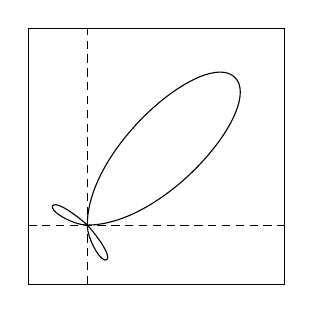
\begin{tikzpicture}[scale=0.25]
			\draw[ultra thin, densely dashed] (0,-3) -- (0,10);
			\draw[ultra thin, densely dashed] (-3,0) -- (10,0);
			\draw (-3,-3) rectangle (10,10);
			
			\coordinate (0) at (0,0);
			\coordinate (1) at (7.5,7.5);
			\coordinate (2) at (-1.75,1);
			\coordinate (3) at (1,-1.75);
			
			\def\dehnungPos{4}
			\def\dehnungNeg{0.75}
			\def\grossSchleife{1.5}
			\def\kleinSchleife{0.25}
			
			\coordinate (ctrl0up) at ($\dehnungPos*(0,1)$);% \fill[red] (ctrl0up) circle[radius=0.1];
			\coordinate (ctrl0right) at ($\dehnungPos*(1,0)$);% \fill[red] (ctrl0right) circle[radius=0.1];
			\coordinate (ctrl0down) at ($\dehnungNeg*(0,-1)$);% \fill[red] (ctrl0down) circle[radius=0.1];
			\coordinate (ctrl0left) at ($\dehnungNeg*(-1,0)$);% \fill[red] (ctrl0left) circle[radius=0.1];
			\coordinate (ctrl0leftUp) at ($\kleinSchleife*(-1,1)$);% \fill[red] (ctrl0leftUp) circle[radius=0.1];
			\coordinate (ctrl0rightDown) at ($\kleinSchleife*(1,-1)$);% \fill[red] (ctrl0rightDown) circle[radius=0.1];
			
			\coordinate (ctrl1up) at ($(1)+\grossSchleife*(-1,1)$);% \fill[green] (ctrl1up) circle[radius=0.1];
			\coordinate (ctrl1down) at ($(1)+\grossSchleife*(1,-1)$);% \fill[green] (ctrl1down) circle[radius=0.1];
			
			\coordinate (ctrl2up) at ($(2)+\kleinSchleife*(1,1)$);% \fill[blue] (ctrl2up) circle[radius=0.1];
			\coordinate (ctrl2down) at ($(2)+\kleinSchleife*(-1,-1)$);% \fill[blue] (ctrl2down) circle[radius=0.1];
			
			\coordinate (ctrl3up) at ($(3)+\kleinSchleife*(1,1)$);% \fill[yellow] (ctrl3up) circle[radius=0.1];
			\coordinate (ctrl3down) at ($(3)+\kleinSchleife*(-1,-1)$);% \fill[yellow] (ctrl3down) circle[radius=0.1];
			
			\path[draw] (0) ..controls(ctrl0up) and (ctrl1up).. (1) ..controls(ctrl1down) and (ctrl0right).. (0) ..controls(ctrl0left) and (ctrl2down).. (2) ..controls(ctrl2up) and (ctrl0leftUp).. (0) ..controls(ctrl0rightDown) and (ctrl3up).. (3) ..controls(ctrl3down) and (ctrl0down).. (0);
		\end{tikzpicture}$\quad$
		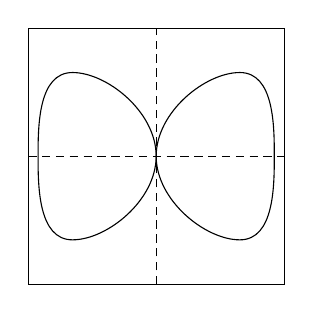
\begin{tikzpicture}[scale=0.25]
			\draw[ultra thin, densely dashed] (0,-6.5) -- (0,6.5);
			\draw[ultra thin, densely dashed] (-6.5,0) -- (6.5,0);
			\draw (-6.5,-6.5) rectangle (6.5,6.5);
			
			\coordinate (0) at (0,0);
			\coordinate (top right) at (4.25,4.25);
			\coordinate (bottom right) at (4.25,-4.25);
			\coordinate (bottom left) at (-4.25,-4.25);
			\coordinate (top left) at (-4.25,4.25);
			\coordinate (right) at (6,0);
			\coordinate (left) at (-6,0);
			
			
			\coordinate (ctrl1) at ($(0)+(0,2.25)$);% \fill[red] (ctrl1) circle[radius=0.1];
			\coordinate (ctrl2) at ($(top right)+(-1.75,0)$);% \fill[red] (ctrl2) circle[radius=0.1];
			\coordinate (ctrl3) at ($(top right)+(top right)-(ctrl2)$);% \fill[red] (ctrl3) circle[radius=0.1];
			\coordinate (ctrl4) at ($(right)+(0,1.5)$);% \fill[red] (ctrl4) circle[radius=0.1];
			
			\coordinate (lrCtrl1) at ($(0)+(0,-2.25)$);
			\coordinate (lrCtrl2) at ($(bottom right)+(-1.75,0)$);
			\coordinate (lrCtrl3) at ($(bottom right)+(bottom right)-(lrCtrl2)$);
			\coordinate (lrCtrl4) at ($(right)-(0,1.5)$);
			
			\coordinate (llCtrl1) at (lrCtrl1);
			\coordinate (llCtrl2) at ($(bottom left)+(1.75,0)$);
			\coordinate (llCtrl3) at ($(bottom left)+(bottom left)-(llCtrl2)$);
			\coordinate (llCtrl4) at ($(left)-(0,1.5)$);
			
			\coordinate (ulCtrl1) at (ctrl1);
			\coordinate (ulCtrl2) at ($(top left)+(1.75,0)$);
			\coordinate (ulCtrl3) at ($(top left)+(bottom left)-(llCtrl2)$);
			\coordinate (ulCtrl4) at ($(left)+(0,1.5)$);
			
			\path[draw] (0) ..controls(ctrl1) and (ctrl2).. (top right) ..controls(ctrl3) and (ctrl4).. (right);
			\path[draw] (0) ..controls(lrCtrl1) and (lrCtrl2).. (bottom right) ..controls(lrCtrl3) and (lrCtrl4).. (right);
			\path[draw] (0) ..controls(llCtrl1) and (llCtrl2).. (bottom left) ..controls(llCtrl3) and (llCtrl4).. (left);
			\path[draw] (0) ..controls(ulCtrl1) and (ulCtrl2).. (top left) ..controls(ulCtrl3) and (ulCtrl4).. (left);
		\end{tikzpicture}$\quad$
		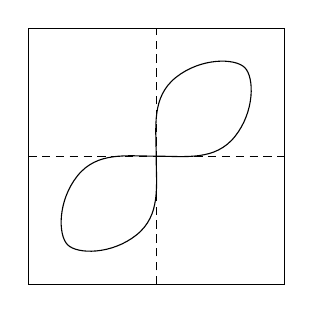
\begin{tikzpicture}[scale=0.25]
			\draw[ultra thin, densely dashed] (0,-6.5) -- (0,6.5);
			\draw[ultra thin, densely dashed] (-6.5,0) -- (6.5,0);
			\draw (-6.5,-6.5) rectangle (6.5,6.5);
			
			\draw (0,0) ..controls(0,1.5) and (-0.25,3).. (1,4) ..controls(2.25,5) and (4,5).. (4.5,4.5) ..controls(5,4) and (5,2.25).. (4,1) ..controls(3,-0.25) and (1.5,0).. (0,0);
			\draw (0,0) ..controls(0,-1.5) and (0.25,-3).. (-1,-4) ..controls(-2.25,-5) and (-4,-5).. (-4.5,-4.5) ..controls(-5,-4) and (-5,-2.25).. (-4,-1) ..controls(-3,0.25) and (-1.5,0).. (0,0);
		\end{tikzpicture}$\quad$
		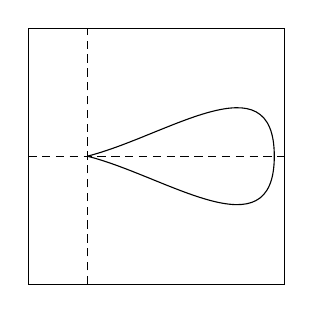
\begin{tikzpicture}[scale=0.25]
			\draw[ultra thin, densely dashed] (0,-6.5) -- (0,6.5);
			\draw[ultra thin, densely dashed] (-3,0) -- (10,0);
			\draw (-3,-6.5) rectangle (10,6.5);
			
			\draw (9.5,0) .. controls(9.5,5) and (4,1) .. (0,0);
			\draw (9.5,0) .. controls(9.5,-5) and (4,-1) .. (0,0);
		\end{tikzpicture}
	\end{center}
\end{enumerate}\end{Aufg}

\begin{Aufg}[4 Punkte]
F"ur diese Aufgabe habe der K"orper $k$ die Charakteristik $0$. Sei $V$ eine projektive Hyperfl"ache in $\Projective^n(k)$, d.h. $V = V(f)$ f"ur ein homogenes, quadratfreies Polynom $f \in k[X_0, \dots, X_n] \setminus k$.
\begin{enumerate}[a)]
	\item Zeige, dass $f \in k[X_0, \dots, X_n] \setminus k$, homogen vom Grad $d$, die folgende Differentialgleichung (von Euler) erf"ullt:  $\sum\limits_{j=0}^n X_j \frac{\partial f}{\partial X_j}=d \cdot f$.
	\item Ein Punkt $x \in V$ ist genau dann singul"ar, wenn $\frac{\partial f}{\partial X_j}(x)=0$ f"ur $j=0, \dots,n$.
	\item Bestimme die singul"aren Punkte der Bernoullischen Lemniskate $$B:=V((X^2+Y^2)^2-2(Y^2Z^2-X^2Z^2)) \subseteq \mathbb{P}^2(k)\,.$$
\end{enumerate}\end{Aufg}

\begin{Aufg}[4 Punkte]
Die Charakteristik von $k$ sei weder $2$ noch $3$. F"ur $\lambda\in k$ betrachten wir die Kurve $E_\lambda = V(Y^2 - X(X-1)(X-\lambda))$.
\begin{enumerate}[a)]
	\item F"ur welche $\lambda$ ist $E_\lambda$ singul"ar?
	
	\emph{Hinweis:} Benutze Aufgabe 1 zur Bestimmung von $I(E_\lambda)$.
	\item Bestimme den projektiven Abschluss $\overline{E_\lambda}$ von $E_\lambda$ und untersuche, ob er singul"are Punkte enth"alt.
	\item Was passiert f"ur $\Char(k) =2$ oder $3$?
\end{enumerate}\end{Aufg}

\begin{Loes}\begin{enumerate}[a)]\item
Die Singularit"aten von $V(XY^2 - Z^2)$ habe ich in der "Ubung berechnet. Bei allen anderen Variet"aten ist $S_f := V(f, \pder{X_1}{f}, \dots, \pder{X_n}{f}) = \{(0,0)\}$ und damit, nach Aufgabe 1, $(0,0)$ die einzige Singularit"at von $V(f)$.
\end{enumerate}\end{Loes}

\setcounter{Loes}{3}

\begin{Loes}
Sei $f:= Y^2 - X(X-1)(X-\lambda) = Y^2- X^3+(\lambda+1)X^2 - \lambda X$.\begin{enumerate}[a)]
\item
	Sei $p=(x,y) \in E_ {\lambda}$. Es gilt $J_f(p) = (-3x^2+2(\lambda+1)x-\lambda, 2y)$ und damit $J_f(p) = (0,0) \Leftrightarrow y = 0 \wedge -3x^2+2(\lambda +1)x - \lambda = 0$. Aus $y = 0$ und $p \in E_\lambda$ folgt $x(x-1)(x-\lambda) = 0$, also $x \in \{0,1,\lambda\}$. Setzen wir das in die zweite Bedingung für $J_f(p) = (0,0)$ ein, so erhalten wir:
	\begin{itemize}
		\item f"ur $x = 0$: $-\lambda = 0 $, also $\lambda = 0$
		\item f"ur $x = 1$: $-3+2(\lambda+1) - \lambda = 0$, also $\lambda = 1$
		\item f"ur $x = \lambda$: $-3 \lambda^2 + 2 (\lambda + 1) \lambda - \lambda = 0 \Leftrightarrow - \lambda^2 + \lambda =  0 \Leftrightarrow \lambda \in \{0,1\}$
	\end{itemize}
	Die Menge $S_f := V(f, \pder{X}{f}, \pder{Y}{f})$ ist folglich f"ur alle $\lambda \in k$ endlich. Mit Aufgabe 1 folgt, dass $I(E_\lambda) = (f)$. Somit ist $E_\lambda$ f"ur $\lambda \notin\{0,1\}$ nichtsingul"ar. F"ur $\lambda = 0$ hat $E_ \lambda$ die Singularit"at $(0,0)$, f"ur $\lambda = 1$ die Singularit"at $(1,0)$.
\item
	In der "Ubung habt ihr mir hoffentlich schon geglaubt, dass $\overline{E_\lambda} =  V (H_Z(f)) = V(ZY^2 - X^3 + (\lambda+1) X^2Z - \lambda X Z^2)$. Weiter ist $\overline{E_\lambda} = (\overline{E_\lambda} \cap D(Z) ) \cup (\overline{E_\lambda} \cap V(Z)) = E_\lambda \cup V(X,Z) = E_\lambda \cup \{(0:1:0)\}$. Alle Punkte aus $E_\lambda$ haben wir schon untersucht (\quot{singul"ar} \, ist eine lokale Eigenschaft). F"ur $p=(0:1:0)$ und $F := H_Z(f)$ gilt
	\begin{eqnarray*}
		(\pder{X}{F})(p) &=& (-3X^2 + 2 (\lambda+1) XZ - \lambda Z^2)(p) = 0 \\
		(\pder{Y}{F})(p) &=&  (2YZ)(p) = 0\\
		(\pder{Z}{F})(p) &=& (Y^2+(\lambda+1)X^2-2 \lambda XZ)(p) = 1 \neq 0
	\end{eqnarray*}
	Somit ist $p$ f"ur alle $\lambda \in k$ nichtsingul"ar und $\overline{E_\lambda}$ hat genau die Singularit"aten von $E_\lambda$.
\item
	Der Punkt $p=(0:1:0)$ im projektiven Abschluss von $E_\lambda$ ist unabh"angig von der Charakteristik nichtsingul"ar. Sei als $p =(x,y) \in E_\lambda$.
	\begin{description}
	\item[$\Char(k)=2:$]
		Hier ist $J_f(p) = (-3x^2-\lambda, 0) = (0,0) \Leftrightarrow x = \pm i \sqrt{\frac{\lambda}{3}}$. Aus $p \in E_\lambda$ folgt $y^2= h(x)$ mit $h(x) = x(x-1)(x-\lambda)$. F"ur $\lambda \neq 0$ ist der Punkt $x= \pm i \sqrt{\frac{\lambda}{3}}$ keine Nullstelle von $h$, also hat $E_\lambda$ die $4$ Singularit"aten
			\[(\, i\sqrt{\frac{\lambda}{3}} , \pm \sqrt{h\left( i \sqrt{\frac{\lambda}{3}} \right)}\,), \quad 
			(\,-i\sqrt{\frac{\lambda}{3}}, \pm \sqrt{h\left(- i \sqrt{\frac{\lambda}{3}}\right)} \,).\]
		F"ur $\lambda = 0$ ist $(0,0)$ die einzige Singularit"at.

		Insgesamt sieht man, dass f"ur $\Char(k) = 2$ alle Kurven $E_\lambda$ singul"ar sind.
	\item[$\Char(k)=3:$]
		Es gilt $J_f(p) = (2(\lambda+1) x - \lambda , 2y) = (0,0) \Leftrightarrow y = 0 \wedge 2 (\lambda+1)x = \lambda$. F"ur $\lambda = -1$ sind diese Bedingungen nicht zu erf"ullen und $E_\lambda$ ist nichtsingul"ar. F"ur $\lambda \neq -1$ erf"ullt $p = ( \frac{\lambda}{2(\lambda+1)},0)$ die Bedingung $J_f(p)=(0,0)$. Einsetzen in $f(p) = 0$ liefert nach etwas Rechnen $\lambda \in \{ -\frac{1}{2},-2\}$. F"ur diese $\lambda$ ist $( \frac{\lambda}{2(\lambda+1)},0)$ eine Singularit"at von $E_\lambda$, f"ur alle anderen $\lambda$ ist $E_\lambda$ nichtsingul"ar.
	\end{description}
\end{enumerate}\end{Loes}

%-------------------------- Uebung 13 --------------------------
\newpage
\section{27. Januar 2011}
\setcounter{Aufg}{0}
\setcounter{Loes}{0}

Auf diesem Blatt bezeichne $k$ immer einen algebraisch abgeschlossenen K"orper.

\begin{Aufg}[5 Punkte]
Seien $X$ und $Y$ quasiprojektive Variet\"aten in $\Projective^n(k)$. Sind die folgenden Aussagen richtig oder falsch? Begr"unde jeweils Deine Antwort.
\begin{enumerate}[a)]
	\item $X,Y$ nichtsingul"ar $\Rightarrow X \cap Y$ nichtsingul"ar.
	\item $X,Y$ nichtsingul"ar $\Rightarrow X \cup Y$ nichtsingul"ar.
	\item $X,Y$ singul"ar $\Rightarrow X \cap Y$ singul"ar.
	\item $X,Y$ singul"ar $\Rightarrow X \cup Y$ singul"ar.
	\item $\emptyset \neq \textrm{Sing}(Y) \subsetneq X \cap Y \Rightarrow X \cap Y$ ist singul"ar.
\end{enumerate}
\emph{Hinweis:} Alle notwendigen Gegenbeispiele k"onnen im affinen Raum gefunden werden.
\end{Aufg}

\begin{Aufg}[4 Punkte]
Es sei $f\in k[X,Y] \setminus k$ ein quadratfreies Polynom und $V = V(f)$. f"ur einen Punkt $p \in V(f)$ definieren wir die Vielfachheit $\mu_p(V)$ in $p$ folgenderma\ss en: 

Es sei $\varphi \colon \Affine^2(k)\to \Affine^2(k)$ eine Translation (d.h. $\varphi(x) = x + t$ f"ur ein $t\in k^2$), so dass $\varphi(p) = (0,0)$ gilt. Wir schreiben $\tilde f = f\circ \varphi^{-1}$ als Summe seiner homogenen Komponenten
	\[\tilde f = \tilde f_0 +\dots + \tilde f_d\,.\]
Dann sei $\mu_p(V) = \min\set{r\in \N_0}{\tilde f_r \neq 0}$.

Zeige, dass $p$ genau dann ein singul"arer Punkt von $V$ ist, wenn $\mu_p(V) > 1$ gilt.

Bestimme die Vielfachheiten der Singularit"aten der Kurven in $\Affine^2(k)$ aus Aufgabe 2 von "Ubungsblatt 12.
\end{Aufg}

\begin{Aufg}[3 Punkte]
Die Charakteristik von $k$ sei $0$. F"ur ein nichtkonstantes Polynom $f\in k[X]$ und eine nat"urliche Zahl $n\geq 1$ sei $C := V(Y^n - f)\subset \Affine^2(k)$. 

F"ur welche $n$ und $f$ ist $C$ eine nichtsingul"are Kurve?
\end{Aufg}

\begin{Aufg}[4 Punkte]
Seien $I_1,\ldots, I_n$ Ideale in einem Ring $R$ und $J \subseteq R$ ein Ideal mit $J \nsubseteq I_i$ für $i=1,\ldots,n$. 

Zeige, dass auch $J \nsubseteq\bigcup_{i=1}^n I_i$ gilt, falls mindestens $n-2$ der Ideale $I_i$ Primideale sind.
\end{Aufg}

%-------------------------- Uebung 14 --------------------------
\newpage
\section{3. Februar 2011}
\setcounter{Aufg}{0}
\setcounter{Loes}{2}

Auf diesem Blatt bezeichne $k$ immer einen algebraisch abgeschlossenen K"orper.

\begin{Aufg}[4 Punkte]
Sei $R$ ein nullteilerfreier, noetherscher Ring mit Quotientenk"orper $K \ne R$. Zeige die "Aquivalenz der folgenden Aussagen:
\begin{enumerate}[i)]
	\item $R$ ist ein diskreter Bewertungsring.
	\item F"ur jedes $x \in K$ gilt $x \in R$ oder $x^{-1} \in R$.
	\item Die Menge der Hauptideale von $R$ ist bez"uglich Inklusion total geordnet.
	\item Die Menge aller Ideale von $R$ ist bez"uglich Inklusion total geordnet.
	\item $R$ ist ein lokaler Hauptidealring.
\end{enumerate}\end{Aufg}

\begin{Aufg}[6 Punkte]
Die Charakteristik von $k$ sei nicht $2$. Wir betrachten $C = V(Y^4 - XZ(X-Z)(X+Z))\subset \Projective^2(k)$.
\begin{enumerate}[a)]
	\item Zeige, dass $C$ eine nichtsingul"are Kurve ist.
	\item Es sei $h:C\to \Projective^1(k)$, $(x:y:z) \mapsto (x:z)$. Bestimme den Grad von $h$ und f"ur jeden Punkt $P\in C$ den Verzweigungsindex $e_P(h)$.
	\item Bestimme die Divisoren der rationalen Funktionen $x/z$ und $x/y\in k(C)$.
\end{enumerate}\end{Aufg}

\begin{Aufg}[6 Punkte]
Es sei $C \subset \Projective^n(k)$ eine irreduzible, nichtsingul"are, projektive Kurve und $G\in k[X_0,\dots,X_n]$ ein homogenes Polynom, so dass $C\not\subset V(G)$ gilt. Wir definieren den Schnittdivisor $\Divisor(G)$ zu $G$ folgenderma\ss en: F"ur einen Punkt $P\in C$ w"ahlen wir ein homogenes Polynom $H\in k[X_0,\dots,X_n]$ mit $H(P)\neq 0$ und $\deg(H) = \deg(G)$ und setzen $n_P = \ord_P(G/H)$. Dann sei $\Divisor(G) = \sum_{P\in C} n_P\cdot P$.
\begin{enumerate}[a)]
\item
	Zeige, dass $\Divisor(G)$ wohldefiniert ist.
\item
	Sei nun $G_1, G_2 \in k[X_0,\dots,X_n]$ mit $\deg(G_1) = \deg(G_2)$. Zeige, dass die zwei Schnittdivisoren $\Divisor(G_1)$ und $\Divisor(G_2)$ linear "aquivalent sind.
\item
	Es sei $\Char(k)\neq 2$. Bestimme f"ur $C= V(Y^2Z - X(X-Z)(X+Z))\subset \Projective^2(k)$ die Schnittdivisoren von $X$, $Y$ und $Z$. Welche geometrische Bedeutung haben diese Divisoren?
\item
	Der Grad $d$ von $C$ sei der Grad des Schnittdivisors eines homogenen Polynoms von Grad 1. Zeige: Ist $n=2$ und $C= V(F)$ für ein homogenes Polynom $F\in k[X_0,X_1,X_2]$, so gilt $\deg(F) = d$.
	
	\emph{Hinweis: Man kann ohne Einschr"ankung voraussetzen, dass $(0:0:1)\not\in V(F)$. (Wieso?) Dann hilft es, den Morphismus $C\to \Projective^1(k)\ ,\ (x:y:z)\mapsto (x:y)$ zu betrachten.}
\item
	Zeige eine Version des Satzes von B\'ezout f"ur nichtsingul"are Kurven: Ist $G\in k[X_0,\dots,X_n]$ ein homogenes Polynom von Grad $e$, so dass $C\not\subset V(G)$, und ist $d$ wieder der Grad von $C$, so gilt
		\[\deg(\Divisor(G)) = d\cdot e.\]
\end{enumerate}\end{Aufg}

\begin{Loes}\begin{enumerate}[a)]
\item
	F"ur $P \in C$, $P = (x_0 \colon \dots \colon x_n)$ gibt es ein $i$ mit $x_i \neq 0$. Also erf"ullt $X_i^{\deg(G)}$ die Bedingungen an $H$. Au\ss erdem ist $C$ echt in $\Projective^n(k)$ enthalten und irreduzibel, also hat $V(G) \cap C$ Dimension $0$ (kleinere Dimension als $C$) und ist somit endlich. Damit ist nur f"ur endlich viele $P \in C$ $\ord_P(G/H) \neq 0$ und die formale Summe in $\Divisor(G)$ endlich.
 
	Es bleibt zu zeigen, dass die Definition nicht von der Wahl von $H$ abh"angt. Sei dazu $H' \in k[X_0, \dots, X_n]$ ein weiteres homogenes Polynom mit $\deg(H') = \deg (G)$ und $H'(P) \neq 0$. Dann ist $\ord_P(G/H) = \ord_P(G/H \cdot H'/H') = \ord_P(G/H') + \ord_P(H'/H)$. Wegen $H'(P) \neq 0$ ist $\ord_P(H'/H) = 0$.
\item
	Wir zeigen $\Divisor(G_1) - \Divisor(G_2) = \Divisor(G_1/G_2)$.

	Sei $P \in C$, $H \in k[X_0, \dots, X_n]$ homogen mit $\deg(H) = \deg(G_i)$ und $H(P) \neq 0$. Es gilt $\ord_P(G_1/G_2) = \ord_P(G_1/H \cdot H /G_2) = \ord_P(G_1/H) - \ord_P(G_2/H)$.
\item
	 Zun"achst berechnen wir die Uniformisierende im Punkt $P = (a : b : c) \in C$, also einen Erzeuger des maximalen Ideals $m_P$ von $\calO_{C,P}$. 
	\begin{description}
	\item[1. Fall:]
		$P \in C \cap D(Z)$, $b \neq 0$.

		Das Ideal $m_P$ wird von $\frac{X}{Z} - \frac{a}{c}$ und $\frac{Y}{Z} - \frac{b}{c}$ erzeugt. Uniformisierende ist $\frac{X}{Z} - \frac{a}{c}$, da 
		\begin{eqnarray*}
			(\frac{Y}{Z} - \frac{b}{c}) \cdot (\frac{Y}{Z} + \frac{b}{c}) 
			&=& \frac{Y^2}{Z^2} - \frac{b^2}{c^2} 
			= \frac{Y^2Z}{Z^3} - \frac{b^2c}{c^3} 
			= \frac{X(X-Z)(X+Z)}{Z^3} - \frac{a(a-c)(a+c)}{c^3}\\
			&=& (\frac{X}{Z} - \frac{a}{c}) (\frac{X^2}{Z^2} + \frac{a}{c} \frac{X}{Z} + \frac{a^2}{c^2} - 1)
		\end{eqnarray*}
		und $\frac{Y}{Z} + \frac{b}{c} \in \calO_{C,P}^\times$ f"ur $b \neq 0$.
	\item[2. Fall:]
		$P \in C \cap D(Z)$, $b = 0$. Hier ist $P \in \{(0:0:1), (1:0:1), (-1:0:1)\}$. Es gilt
			\[\frac{Y^2}{Z^2} = \frac{Y^2Z}{Z^3} = \frac{X(X-Z)(X+Z)}{Z^3} = \frac{X}{Z} (\frac{X}{Z} -1)(\frac{X}{Z} +1)\,.\]
		F"ur $P = (0:0:1)$ sind $\frac{X}{Z} -1 \in \calO_{C,P}^\times$ und $\frac{X}{Z} +1 \in \calO_{C,P}^\times$, also ist $\frac{X}{Z} = \frac{1}{(\frac{X}{Z} -1)(\frac{X}{Z} +1)} \frac{Y^2}{Z^2} \in (\frac{Y}{Z})$. Analog sind f"ur $P = (1:0:1)$ bzw. $P = (-1:0:1)$ die Erzeuger $\frac{X}{Z} - 1 = \frac{1}{\frac{X}{Z}(\frac{X}{Z} +1)} \frac{Y^2}{Z^2} \in \left(\frac{Y}{Z}\right)$ bzw. $\frac{X}{Z} + 1 = \frac{1}{\frac{X}{Z}(\frac{X}{Z} - 1)} \frac{Y^2}{Z^2} \in \left(\frac{Y}{Z}\right)$.

		Das maximale Ideal $m_P$ wird folglich von $\frac{Y}{Z}$ erzeugt. 
	\item[3. Fall:]
		$P = (0:1:0)$
		
		Es gilt $\frac{Z}{Y} = \frac{Y^2Z}{Y^3} = \frac{X(X-Z)(X+Z)}{Y^3} = \frac{X^3}{Y^3} - \frac{XZ \cdot Z}{Y^2 \cdot Y}$ und somit $\frac{Z}{Y} (1 + \frac{XZ}{Y^2}) = (\frac{X}{Y})^3 $. Da $1 + \frac{XZ}{Y^2} \in \calO_{C,P}^\times$ folgt $\frac{Z}{Y} \in \left(\frac{X}{Y}\right)$ und damit $m_P = \left(\frac{X}{Y} \right)$.
	\end{description}
	Nun k"onnen wir die Schnittdivisoren berechnen: 

	Zun"achst stellen wir fest, dass $\ord_{(a:b:c)}(\frac{X}{H}) = 0$ für $a \neq 0$. Aus $(0:b:c) \in C$ folgt $b=0$ oder $c=0$. Somit gilt
		\[\Divisor(X) = \ord_{(0:0:1)}(\frac{X}{Z}) \cdot (0:0:1) + \ord_{(0:1:0)}(\frac{X}{Y}) \cdot (0:1:0) = 2 \cdot (0:0:1) + 1 \cdot (0:1:0)\; .\]
	Analog folgt
		\[\Divisor(Y) = 1 \cdot (0:0:1) +  1 \cdot (1:0:1) +  1 \cdot (-1:0:1) \quad \textrm{und} \quad
		\Divisor(Z) = 3 \cdot (0:1:0)\;.\]
 	Die geometrische Bedeutung des Schnittdivisors ist genau das, was der Name suggeriert. Schneidet man $C$ mit $V(G)$ und z"ahlt die Schnittpunkte mit Vielfachheit, so bekommt man den Schnittdivisor $\Divisor(G)$. Die Abbildungen 1 und 2 zeigen zwei reelle Bilder zur geometrischen Bedeutung.
	\begin{center}
		\textcolor{red}{[BILD]}\\
		Abbildung 1: $C \cap D(Z)$ mit $V(X)$ ($y$-Achse) und $V(Y)$ ($x$-Achse).

		\textcolor{red}{[BILD]}\\
		Abbildung 2: $C\cap D(Y)$ mit $V(Z)$ ($x$-Achse).
	\end{center}
\item
	Es gibt ein $P =(a:b:c)\in \Projective^2\setminus V(F)$ und eine lineare Abbildung $\Phi \in \GL_3(k)$ mit $\Phi(a,b,c) = (0,0,1)$. Dieses $\Phi$ induziert einen Isomorphismus $\tilde{\Phi} \colon V(F) \to V(\tilde{F})$, $(x:y:z) \mapsto \Phi(x:y:z)$, wobei $\tilde{F} = F \circ \Phi^{-1}$ (etwas sehrr "ahnliches haben wir auf "Ubungsblatt 13 in Aufgabe 2 schon einmal gemacht). Wegen $\tilde{F}((0:0:1)) = (F \circ \Phi^{-1})((0:0:1)) = F((a:b:c)) \neq 0$ ist $(0:0:1)$ nicht in $V(\tilde{F})$ enthalten. Folglich gilt ohne Einschr"ankung, dass $(0:0:1) \notin C$.

	Wir betrachten den Morphismus $h: C \to \Projective^1(k), (x:y:z) \mapsto(x:y)$. Dieser ist wohldefiniert, da $(0:0:1) \notin C$.

	\emph{Behauptung 1:} $\Divisor(X) = h^\ast((0:1))$.

	\emph{Beweis Beh. 1:} Sei $P\in C$. Ist $P \in D(Y)$, so gilt $\ord_P(\Divisor(X)) = \ord_P(\frac{X}{Y}) = \ord_P(\frac{X_0}{X_1} \circ h) = e_P(h) = \ord_P(h^\ast(0:1))$. Ist andernfalls $P = (a:0:c) \in V(Y)$, dann ist $h(P) \neq (0:1)$ und damit $\ord_P(h^\ast(0:1)) = 0$. A\ss erdem folgt aus $(0:0:1)\notin C$, dass $a \neq 0$ und damit $\ord_P(\Divisor(X)) = 0$.

	\emph{Behauptung 2:} $\deg h = \deg F$. 

	Aus Behauptung 1 und 2 folgt dann wie gew"unscht 
		\[d = \deg(\Divisor(X)) = \deg(h^\ast((0:1))) = \sum_{h(P) = (0:1)} e_P(h) = \deg h = \deg F \, .\]

	\emph{Beweis Beh. 2:} Nach Definition gilt $\deg h = [k(C) : k(\Projective^1(k))]$. Betrachte die Einschr"ankung $h^a$ von $h$ auf $C^a = C \cap D(Y)$ nach $\Projective^1(k) \cap D(Y) = \Affine^1(k)$. Der Morphismus $h^a: C^a \to \Affine^1(k), (x:1:z) \mapsto x$ induziert einen Morphismus $(h^a)^\sharp: k(\Affine^1(k)) = k(X) \hookrightarrow k(C^a) = k(x,z), X \mapsto x$, wobei $x$ und $z$ die Restklassen von $X$ und $Z$ in $k[C^a]$ bezeichnen. 
 
	Das Bild von $(h^a)^\sharp$ ist $k(x)$ und f"ur $z$ gilt $F(x,1,z) = 0$. Sei $m$ der Grad von $F$ und $F = \sum_{i+j+k=m} a_{ijk} X^i Y^j Z ^k$. Wegen $(0:0:1) \notin C$ ist $a_{00m} \neq 0$ und die Dehomogenisierung von $F$ nach $Y$, $f := F(X,1,Z)$, hat Grad $m$ in $Z$. Da $F$ irreduzibel in $k[X,Y,Z]$ ist, ist auch $f$ irreduzibel in $k[X,Z]$. Eine einfache Folgerung aus dem Lemma von Gau\ss \footnote{siehe Hilfssatz 2.2.6 in \quot{Algebra im WS 2011/2012} von Dr. Stefan K"uhnlein} sagt, dass dann $f$ auch "uber $k(X)[Z]$ irreduzibel ist. Wegen $C^a = V(f)$, gilt $k(C^a) = \Quot(k[X,Z]/(f)) \isom k(X)[Z] / (f)$ und somit $\deg h^a  = [k(C^a) : k(X)] = \deg f $.
	
	Die Inklusion $C^a \hookrightarrow C$ hat eine dominante rationale Umkehrabbildung $\id \colon C \dashrightarrow C^a$. Daher ist $k(C^a ) \isom k(C)$. Genauso ist auch $k(\Projective^1(k)) \isom k(\Affine^1(k))$ und es folgt $\deg h = [k(C) : k(\Projective^1(k))] = [k(C^a) : k(\Affine^1(k))] = \deg h^a$. Insgesamt gilt $\deg F = \deg f = \deg h^a = \deg h$.
\item
	Sei $H \in K[X_0, \dots, X_n]$ homogen, $\deg(H) = 1$, $C \nsubset V(H)$ (z.B. $H = X_i$). Dann ist $\deg(G) = \deg(H^e)$. Nach b) sind $\Divisor(G)$ und $\Divisor(H^e)$ linear "Aquivalent, es gilt also $\deg(\Divisor(G)) = \deg(\Divisor(H^e))$. Weiterhin gilt $\deg(\Divisor(H^e)) = e \cdot \deg(\Divisor(H))) = e \cdot d$, denn $\ord_P(\Divisor(H)) = n_P \Leftrightarrow \ord_P(H / \tilde{H}) = n_P$, wobei $\tilde{H} \in k[X_0, \dots, X_n]$ mit $\deg(\tilde{H}) = 1$ und $\tilde{H}(P) \neq 0$ und damit $\ord_P(\Divisor(H^e)) = \ord_P(H^e / \tilde{H}^e) = e \cdot \ord_P(H / \tilde{H}) = e \cdot n_P$.
\end{enumerate}\end{Loes}


%-_-_-_-_-_-_-_-_-_-_-_-_-_-_ Stichwortverzeichnis -_-_-_-_-_-_-_-_-_-_-_-_-_-_-_-_

\def\indexspace{\par\medskip}
\printindex[default][\phantomsection\addcontentsline{toc}{chapter}{Stichwortverzeichnis}\vspace{-1.2em}]


%--------------------------Gaestebuch----------------------------


\chapter{G\"astebuch}
Hier kann jeder, der g\"o\ss ere \"Anderungen oder Korrekturen am Skript vorgenommen hat, seinen Namen und einen Kommentar hinterlassen. Kleinigkeiten wie Rechtschreibfehler m\"ussen nicht unbedingt sein (und bei meinen Tippfehlern w\"are das G\"astebuch gr\"o\ss er als das Skript), aber ein korrigierter Satz, ein vervollst\"andigter Beweis, solche Sachen, einfach damit jemand der eine \"altere Version des Skriptes hat schnell den Unterschied finden kann. Oder hinterlasst einfach ein Paar nette Worte :-)\\
Zum Schreiben im G\"astebuch stehen euch folgende Umgebungen zur Verf\"ugung (neben den \"ublichen aus dem Skript):
\begin{center}\begin{minipage}{0.3\textwidth}\begin{verbatim}
	\begin{gast}
		...
	\end{gast}
\end{verbatim}\end{minipage}
\begin{minipage}{0.3\textwidth}\begin{verbatim}	
	\begin{komm}
		...	
	\end{komm}
\end{verbatim}\end{minipage}
\begin{minipage}{0.3\textwidth}\begin{verbatim}	
	\begin{korr}
		...	
	\end{korr}
\end{verbatim}\end{minipage}\end{center}
G\"astebucheintr\"age sind f\"ur alle Arten von Eintr\"agen gedacht. Kommentare sollten nur f\"ur wichtige Sachen verwendet werden und auch blo\ss,  wenn man sie nicht direkt in das Skript einbauen kann. Korrekturen sind da um gr\"o\ss ere und wichtige Korrekturen festzuhalten, damit man schnell wei\ss was sich seit der letzten Version wichtiges ge\"andert hat.\\
Dieser Teil ist absichtlich am Ende, damit man ihn beim Drucken einfach weglassen kann. Wenn jemand einen weiteren Anhang einf\"ugen m\"ochte, dann tut das bitte \emph{vor} dem G\"astebuch.\\

\begin{gast}[von Aleks am 23. April 2012]
Ich habe das G\"astebuch angelegt. Ihr k\"onnt hier Aufz\"ahlungen verwenden:
\begin{enumerate}[1)]
\item
	Ist das nicht toll?
\item
	Ich kann sogar einen Link zu einem Eintrag setzen, wie zum Beispiel Folgerung \ref{folg1.2}
\end{enumerate}
\end{gast}

\begin{gast}[Chris]
Dankbar mit dem Skript gearbeitet und durchkorrigiert (kleinere Fehler und ein paar Sachen erg\"anzt).\\
Mir sind noch ein paar Sachen aufgefallen, an die ich mich ohne Originalmitschrieb nicht dran traute (s. auch meine LaTeX-F\"ahigkeiten) (kann man, wenn korrigiert, l"oschen):
\begin{itemize}
\item Bew. von Satz 3 steht Zeile doppelt und die Nummerierung ist seltsam (hab grad keinen Aufschrieb da); an der Stelle ist noch mehr vermurkst
\item \ref{prop8.6} fehlt Bew.: k\"onnte z.B. so gehn: \quot{$ \Leftarrow $} Seien $g,h \in k[W]: g \circ f=h \circ f \Rightarrow g(f(x))=h(f(x)) \forall x \in V f(V) dicht \Rightarrow g=h    \quot{\Rightarrow} Ang. f nicht dom. \Rightarrow I(f(V))\neq {0} \Rightarrow \exists g \neq 0 \in I und g \circ f=0 Wid. zu inj.$
\item Bew. von 10.6 k\"onnte man auf aff. Variet\"aten verweisen, so ist da noch ne L\"ucke (mit dem Verweis, w\"ar die geschlossen)
\item Bew. Satz 7 a) 2. Beh. etwas aufpassen bei $k[V]_d * f^j$, eigentlich ist es viel eher $k[X_n1,...,X_nm]$ wobei $U_nl \cap D(f) \neq \emptyset$ sein muss!
\end{itemize}
\end{gast}

\end{document}
